%&preformat-disser
\RequirePackage[l2tabu,orthodox]{nag} % Раскомментировав, можно в логе получать рекомендации относительно правильного использования пакетов и предупреждения об устаревших и нерекомендуемых пакетах
% Формат А4, 14pt (ГОСТ Р 7.0.11-2011, 5.3.6)
\documentclass[a4paper,14pt,oneside,openany]{memoir}

%%%%%%%%%%%%%%%%%%%%%%%%%%%%%%%%%%%%%%%%%%%%%%%%%%%%%%%%%%%%%%%%%%%%%%%%%%%%%%%%
%%%% Файл упрощённых настроек шаблона, общих для диссертации и автореферата %%%%
%%%%%%%%%%%%%%%%%%%%%%%%%%%%%%%%%%%%%%%%%%%%%%%%%%%%%%%%%%%%%%%%%%%%%%%%%%%%%%%%

%%% Режим черновика %%%
\makeatletter
\@ifundefined{c@draft}{
  \newcounter{draft}
  \setcounter{draft}{0}  % 0 --- чистовик (максимальное соблюдение ГОСТ)
                         % 1 --- черновик (отклонения от ГОСТ, но быстрая
                         %       сборка итоговых PDF)
}{}
\makeatother

%%% Пометки в тексте %%%
\makeatletter
\@ifundefined{c@showmarkup}{
  \newcounter{showmarkup}
  \setcounter{showmarkup}{0}  % 0 --- скрыть пометки
                              % 1 --- показывать пометки
}{}
\makeatother

%%% Использование в pdflatex шрифтов не по-умолчанию %%%
\makeatletter
\@ifundefined{c@usealtfont}{
  \newcounter{usealtfont}
  \setcounter{usealtfont}{1}    % 0 --- шрифты на базе Computer Modern
                                % 1 --- использовать пакет pscyr, при его
                                %       наличии
                                % 2 --- использовать пакет XCharter, при наличии
                                %       подходящей версии
}{}
\makeatother

%%% Использование в xelatex и lualatex семейств шрифтов %%%
\makeatletter
\@ifundefined{c@fontfamily}{
  \newcounter{fontfamily}
  \setcounter{fontfamily}{1}  % 0 --- CMU семейство. Используется как fallback;
                              % 1 --- Шрифты от MS (Times New Roman и компания)
                              % 2 --- Семейство Liberation
}{}
\makeatother

%%% Библиография %%%
\makeatletter
\@ifundefined{c@bibliosel}{
  \newcounter{bibliosel}
  \setcounter{bibliosel}{1}   % 0 --- встроенная реализация с загрузкой файла
                              %       через движок bibtex8;
                              % 1 --- реализация пакетом biblatex через движок
                              %       biber
}{}
\makeatother

%%% Вывод типов ссылок в библиографии %%%
\makeatletter
\@ifundefined{c@mediadisplay}{
  \newcounter{mediadisplay}
  \setcounter{mediadisplay}{0}   % 0 --- не делать ничего; надписи [Текст] и
                                 %       [Эл. ресурс] будут выводиться только в ссылках с
                                 %       заполненным полем `media`;
                                 % 1 --- автоматически добавлять надпись [Текст] к ссылкам с
                                 %       незаполненным полем `media`; таким образом, у всех
                                 %       источников будет указан тип, что соответствует
                                 %       требованиям ГОСТ
                                 % 2 --- автоматически удалять надписи [Текст], [Эл. Ресурс] и др.;
                                 %       не соответствует ГОСТ
                                 % 3 --- автоматически удалять надпись [Текст];
                                 %       не соответствует ГОСТ
                                 % 4 --- автоматически удалять надпись [Эл. Ресурс];
                                 %       не соответствует ГОСТ
}{}
\makeatother

%%% Предкомпиляция tikz рисунков для ускорения работы %%%
\makeatletter
\@ifundefined{c@imgprecompile}{
  \newcounter{imgprecompile}
  \setcounter{imgprecompile}{0}   % 0 --- без предкомпиляции;
                                  % 1 --- пользоваться предварительно
                                  %       скомпилированными pdf вместо генерации
                                  %       заново из tikz
}{}
\makeatother
            % общие настройки шаблона
\input{common/packages}         % Пакеты общие для диссертации и автореферата
\synopsisfalse                      % Этот документ --- не автореферат
\input{Dissertation/dispackages}    % Пакеты для диссертации
\input{Dissertation/userpackages}   % Пакеты для специфических пользовательских задач

%%%%%%%%%%%%%%%%%%%%%%%%%%%%%%%%%%%%%%%%%%%%%%%%%%%%%%%
%%%% Файл упрощённых настроек шаблона автореферата %%%%
%%%%%%%%%%%%%%%%%%%%%%%%%%%%%%%%%%%%%%%%%%%%%%%%%%%%%%%

%%% Инициализирование переменных, не трогать!  %%%
\newcounter{showperssign}
\newcounter{showsecrsign}
\newcounter{showopplead}
%%%%%%%%%%%%%%%%%%%%%%%%%%%%%%%%%%%%%%%%%%%%%%%%%%%%%%%

%%% Список публикаций %%%
\makeatletter
\@ifundefined{c@usefootcite}{
  \newcounter{usefootcite}
  \setcounter{usefootcite}{0} % 0 --- два списка литературы;
                              % 1 --- список публикаций автора + цитирование
                              %       других работ в сносках
}{}
\makeatother

\makeatletter
\@ifundefined{c@bibgrouped}{
  \newcounter{bibgrouped}
  \setcounter{bibgrouped}{1}  % 0 --- единый список работ автора;
                              % 1 --- сгруппированные работы автора
}{}
\makeatother

%%% Область упрощённого управления оформлением %%%

%% Управление зазором между подрисуночной подписью и основным текстом %%
\setlength{\belowcaptionskip}{10pt plus 20pt minus 2pt}


%% Подпись таблиц %%

% смещение строк подписи после первой
\newcommand{\tabindent}{0cm}

% тип форматирования таблицы
% plain --- название и текст в одной строке
% split --- название и текст в разных строках
\newcommand{\tabformat}{plain}

%%% настройки форматирования таблицы `plain'

% выравнивание по центру подписи, состоящей из одной строки
% true  --- выравнивать
% false --- не выравнивать
\newcommand{\tabsinglecenter}{false}

% выравнивание подписи таблиц
% justified   --- выравнивать как обычный текст
% centering   --- выравнивать по центру
% centerlast  --- выравнивать по центру только последнюю строку
% centerfirst --- выравнивать по центру только первую строку
% raggedleft  --- выравнивать по правому краю
% raggedright --- выравнивать по левому краю
\newcommand{\tabjust}{justified}

% Разделитель записи «Таблица #» и названия таблицы
\newcommand{\tablabelsep}{~\cyrdash\ }

%%% настройки форматирования таблицы `split'

% положение названия таблицы
% \centering   --- выравнивать по центру
% \raggedleft  --- выравнивать по правому краю
% \raggedright --- выравнивать по левому краю
\newcommand{\splitformatlabel}{\raggedleft}

% положение текста подписи
% \centering   --- выравнивать по центру
% \raggedleft  --- выравнивать по правому краю
% \raggedright --- выравнивать по левому краю
\newcommand{\splitformattext}{\raggedright}

%% Подпись рисунков %%
%Разделитель записи «Рисунок #» и названия рисунка
\newcommand{\figlabelsep}{~\cyrdash\ }  % (ГОСТ 2.105, 4.3.1)
                                        % "--- здесь не работает

%Демонстрация подписи диссертанта на автореферате
\setcounter{showperssign}{1}  % 0 --- не показывать;
                              % 1 --- показывать
%Демонстрация подписи учёного секретаря на автореферате
\setcounter{showsecrsign}{1}  % 0 --- не показывать;
                              % 1 --- показывать
%Демонстрация информации об оппонентах и ведущей организации на автореферате
\setcounter{showopplead}{1}   % 0 --- не показывать;
                              % 1 --- показывать

%%% Цвета гиперссылок %%%
% Latex color definitions: http://latexcolor.com/
\definecolor{linkcolor}{rgb}{0.9,0,0}
\definecolor{citecolor}{rgb}{0,0.6,0}
\definecolor{urlcolor}{rgb}{0,0,1}
%\definecolor{linkcolor}{rgb}{0,0,0} %black
%\definecolor{citecolor}{rgb}{0,0,0} %black
%\definecolor{urlcolor}{rgb}{0,0,0} %black
      % Упрощённые настройки шаблона

\input{common/newnames}         % Новые переменные, для всего проекта

%%% Основные сведения %%%
\newcommand{\thesisAuthorLastName}{Манолов}
\newcommand{\thesisAuthorOtherNames}{Александр Иванович}
\newcommand{\thesisAuthorInitials}{А.\,И.}
\newcommand{\thesisAuthor}             % Диссертация, ФИО автора
{%
    \texorpdfstring{% \texorpdfstring takes two arguments and uses the first for (La)TeX and the second for pdf
        \thesisAuthorLastName~\thesisAuthorOtherNames% так будет отображаться на титульном листе или в тексте, где будет использоваться переменная
    }{%
        \thesisAuthorLastName, \thesisAuthorOtherNames% эта запись для свойств pdf-файла. В таком виде, если pdf будет обработан программами для сбора библиографических сведений, будет правильно представлена фамилия.
    }
}
\newcommand{\thesisAuthorShort}        % Диссертация, ФИО автора инициалами
{\thesisAuthorInitials~\thesisAuthorLastName}
%\newcommand{\thesisUdk}                % Диссертация, УДК
%{\fixme{xxx.xxx}}
\newcommand{\thesisTitle}              % Диссертация, название
{Биоинформатический анализ изменчивости генного состава
прокариот, в том числе в ассоциации с патогенностью}
\newcommand{\thesisSpecialtyNumber}    % Диссертация, специальность, номер
{1.5.8}
\newcommand{\thesisSpecialtyTitle}     % Диссертация, специальность, название (название взято с сайта ВАК для примера)
{Математическая биология, биоинформатика}
%% \newcommand{\thesisSpecialtyTwoNumber} % Диссертация, вторая специальность, номер
%% {\fixme{XX.XX.XX}}
%% \newcommand{\thesisSpecialtyTwoTitle}  % Диссертация, вторая специальность, название
%% {\fixme{Теория и~методика физического воспитания, спортивной тренировки,
%% оздоровительной и~адаптивной физической культуры}}
\newcommand{\thesisDegree}             % Диссертация, ученая степень
{кандидата биологических наук}
\newcommand{\thesisDegreeShort}        % Диссертация, ученая степень, краткая запись
{канд. биол. наук}
\newcommand{\thesisCity}               % Диссертация, город написания диссертации
{Москва}
\newcommand{\thesisYear}               % Диссертация, год написания диссертации
{\the\year}
\newcommand{\thesisOrganization}       % Диссертация, организация
{Федеральное государственное бюджетное учреждение "Федеральный научно-клинический центр физико-химической медицины Федерального медико-биологического агентства"}
\newcommand{\thesisOrganizationShort}  % Диссертация, краткое название организации для доклада
{ФГБУ ФНКЦ ФХМ ФМБА России}

\newcommand{\thesisInOrganization}     % Диссертация, организация в предложном падеже: Работа выполнена в ...
{Федеральном государственном бюджетном учреждении "Федеральный научно-клинический центр физико-химической медицины Федерального медико-биологического агентства"}

%% \newcommand{\supervisorDead}{}           % Рисовать рамку вокруг фамилии
\newcommand{\supervisorFio}              % Научный руководитель, ФИО
{Ильина Елена Николаевна}
\newcommand{\supervisorRegalia}          % Научный руководитель, регалии
{доктор биологических наук, член-корреспондент РАН}
\newcommand{\supervisorFioShort}         % Научный руководитель, ФИО
{Е.\,Н.~Ильина}
\newcommand{\supervisorRegaliaShort}     % Научный руководитель, регалии
{д.б.н., чл.-корр. РАН}
%% \newcommand{\supervisorTwoDead}{}        % Рисовать рамку вокруг фамилии
%% \newcommand{\supervisorTwoFio}           % Второй научный руководитель, ФИО
%% {\fixme{Фамилия Имя Отчество}}
%% \newcommand{\supervisorTwoRegalia}       % Второй научный руководитель, регалии
%% {\fixme{уч. степень, уч. звание}}
%% \newcommand{\supervisorTwoFioShort}      % Второй научный руководитель, ФИО
%% {\fixme{И.\,О.~Фамилия}}
%% \newcommand{\supervisorTwoRegaliaShort}  % Второй научный руководитель, регалии
%% {\fixme{уч.~ст.,~уч.~зв.}}

\newcommand{\opponentOneFio}           % Оппонент 1, ФИО
{\fixme{Фамилия Имя Отчество}}
\newcommand{\opponentOneRegalia}       % Оппонент 1, регалии
{\fixme{доктор физико-математических наук, профессор}}
\newcommand{\opponentOneJobPlace}      % Оппонент 1, место работы
{\fixme{Не очень длинное название для места работы}}
\newcommand{\opponentOneJobPost}       % Оппонент 1, должность
{\fixme{старший научный сотрудник}}

\newcommand{\opponentTwoFio}           % Оппонент 2, ФИО
{\fixme{Фамилия Имя Отчество}}
\newcommand{\opponentTwoRegalia}       % Оппонент 2, регалии
{\fixme{кандидат физико-математических наук}}
\newcommand{\opponentTwoJobPlace}      % Оппонент 2, место работы
{\fixme{Основное место работы c длинным длинным длинным длинным названием}}
\newcommand{\opponentTwoJobPost}       % Оппонент 2, должность
{\fixme{старший научный сотрудник}}

%% \newcommand{\opponentThreeFio}         % Оппонент 3, ФИО
%% {\fixme{Фамилия Имя Отчество}}
%% \newcommand{\opponentThreeRegalia}     % Оппонент 3, регалии
%% {\fixme{кандидат физико-математических наук}}
%% \newcommand{\opponentThreeJobPlace}    % Оппонент 3, место работы
%% {\fixme{Основное место работы c длинным длинным длинным длинным названием}}
%% \newcommand{\opponentThreeJobPost}     % Оппонент 3, должность
%% {\fixme{старший научный сотрудник}}

\newcommand{\leadingOrganizationTitle} % Ведущая организация, дополнительные строки. Удалить, чтобы не отображать в автореферате
{Федеральное государственное бюджетное образовательное учреждение высшего
профессионального образования с~длинным длинным длинным длинным названием}

\newcommand{\defenseDate}              % Защита, дата
{\fixme{DD mmmmmmmm YYYY~г.~в~XX часов}}
\newcommand{\defenseCouncilNumber}     % Защита, номер диссертационного совета
{\fixme{Д\,123.456.78}}
\newcommand{\defenseCouncilTitle}      % Защита, учреждение диссертационного совета
{\fixme{Название учреждения}}
\newcommand{\defenseCouncilAddress}    % Защита, адрес учреждение диссертационного совета
{\fixme{Адрес}}
\newcommand{\defenseCouncilPhone}      % Телефон для справок
{\fixme{+7~(0000)~00-00-00}}

\newcommand{\defenseSecretaryFio}      % Секретарь диссертационного совета, ФИО
{\fixme{Фамилия Имя Отчество}}
\newcommand{\defenseSecretaryRegalia}  % Секретарь диссертационного совета, регалии
{\fixme{д-р~физ.-мат. наук}}            % Для сокращений есть ГОСТы, например: ГОСТ Р 7.0.12-2011 + http://base.garant.ru/179724/#block_30000

\newcommand{\synopsisLibrary}          % Автореферат, название библиотеки
{\fixme{Название библиотеки}}
\newcommand{\synopsisDate}             % Автореферат, дата рассылки
{\fixme{DD mmmmmmmm}\the\year~года}

% To avoid conflict with beamer class use \providecommand
\providecommand{\keywords}%            % Ключевые слова для метаданных PDF диссертации и автореферата
{}
             % Основные сведения
\input{common/fonts}            % Определение шрифтов (частичное)
\input{common/styles}           % Стили общие для диссертации и автореферата
\input{Dissertation/disstyles}  % Стили для диссертации
\input{Dissertation/userstyles} % Стили для специфических пользовательских задач

%%% Библиография. Выбор движка для реализации %%%
% Здесь только проверка установленного ключа. Сама настройка выбора движка
% размещена в common/setup.tex
\ifnumequal{\value{bibliosel}}{0}{%
    \input{biblio/predefined}   % Встроенная реализация с загрузкой файла через движок bibtex8
}{
    %%% Реализация библиографии пакетами biblatex и biblatex-gost с использованием движка biber %%%

\usepackage{csquotes} % biblatex рекомендует его подключать. Пакет для оформления сложных блоков цитирования.
%%% Загрузка пакета с основными настройками %%%
\makeatletter
\ifnumequal{\value{draft}}{0}{% Чистовик
\usepackage[%
backend=biber,% движок
bibencoding=utf8,% кодировка bib файла
sorting=none,% настройка сортировки списка литературы
style=gost-numeric,% стиль цитирования и библиографии (по ГОСТ)
language=autobib,% получение языка из babel/polyglossia, default: autobib % если ставить autocite или auto, то цитаты в тексте с указанием страницы, получат указание страницы на языке оригинала
autolang=other,% многоязычная библиография
clearlang=true,% внутренний сброс поля language, если он совпадает с языком из babel/polyglossia
defernumbers=true,% нумерация проставляется после двух компиляций, зато позволяет выцеплять библиографию по ключевым словам и нумеровать не из большего списка
sortcites=true,% сортировать номера затекстовых ссылок при цитировании (если в квадратных скобках несколько ссылок, то отображаться будут отсортированно, а не абы как)
doi=false,% Показывать или нет ссылки на DOI
isbn=false,% Показывать или нет ISBN, ISSN, ISRN
]{biblatex}[2016/09/17]
\ltx@iffilelater{biblatex-gost.def}{2017/05/03}%
{\toggletrue{bbx:gostbibliography}%
\renewcommand*{\revsdnamepunct}{\addcomma}}{}
}{%Черновик
\usepackage[%
backend=biber,% движок
bibencoding=utf8,% кодировка bib файла
sorting=none,% настройка сортировки списка литературы
% defernumbers=true, % откомментируйте, если требуется правильная нумерация ссылок на литературу в режиме черновика. Замедляет сборку
]{biblatex}[2016/09/17]%
}
\makeatother

\providebool{blxmc} % biblatex version needs and has MakeCapital workaround
\boolfalse{blxmc} % setting our new boolean flag to default false
\ifxetexorluatex
\else
% Исправление случая неподдержки знака номера в pdflatex
    \DefineBibliographyStrings{russian}{number={\textnumero}}

% Исправление случая отсутствия прописных букв в некоторых случаях
% https://github.com/plk/biblatex/issues/960#issuecomment-596658282
    \ifdefmacro{\ExplSyntaxOn}{}{\usepackage{expl3}}
    \makeatletter
    \ltx@ifpackagelater{biblatex}{2020/02/23}{
    % Assuming this version of biblatex defines MakeCapital correctly
    }{
        \ltx@ifpackagelater{biblatex}{2019/12/01}{
            % Assuming this version of biblatex defines MakeCapital incorrectly
            \usepackage{expl3}[2020/02/25]
            \@ifpackagelater{expl3}{2020/02/25}{
                \booltrue{blxmc} % setting our new boolean flag to true
            }{}
        }{}
    }
    \makeatother
    \ifblxmc
        \typeout{Assuming this version of biblatex defines MakeCapital
        incorrectly}
        \usepackage{xparse}
        \makeatletter
        \ExplSyntaxOn
        \NewDocumentCommand \blx@maketext@lowercase {m}
          {
            \text_lowercase:n {#1}
          }

        \NewDocumentCommand \blx@maketext@uppercase {m}
          {
            \text_uppercase:n {#1}
          }

        \RenewDocumentCommand \MakeCapital {m}
          {
            \text_titlecase_first:n {#1}
          }
        \ExplSyntaxOff

        \protected\def\blx@biblcstring#1#2#3{%
          \blx@begunit
          \blx@hyphenreset
          \blx@bibstringsimple
          \lowercase{\edef\blx@tempa{#3}}%
          \ifcsundef{#2@\blx@tempa}
            {\blx@warn@nostring\blx@tempa
             \blx@endnounit}
            {#1{\blx@maketext@lowercase{\csuse{#2@\blx@tempa}}}%
             \blx@endunit}}

        \protected\def\blx@bibucstring#1#2#3{%
          \blx@begunit
          \blx@hyphenreset
          \blx@bibstringsimple
          \lowercase{\edef\blx@tempa{#3}}%
          \ifcsundef{#2@\blx@tempa}
            {\blx@warn@nostring\blx@tempa
             \blx@endnounit}
            {#1{\blx@maketext@uppercase{\csuse{#2@\blx@tempa}}}%
             \blx@endunit}}
        \makeatother
    \fi
\fi

\ifsynopsis
\ifnumgreater{\value{usefootcite}}{0}{
    \ExecuteBibliographyOptions{autocite=footnote}
    \newbibmacro*{cite:full}{%
        \printtext[bibhypertarget]{%
            \usedriver{%
                \DeclareNameAlias{sortname}{default}%
            }{%
                \thefield{entrytype}%
            }%
        }%
        \usebibmacro{shorthandintro}%
    }
    \DeclareCiteCommand{\smartcite}[\mkbibfootnote]{%
        \usebibmacro{prenote}%
    }{%
        \usebibmacro{citeindex}%
        \usebibmacro{cite:full}%
    }{%
        \multicitedelim%
    }{%
        \usebibmacro{postnote}%
    }
}{}
\fi

%%% Подключение файлов bib %%%
\addbibresource[label=bl-external]{biblio/external.bib}
\addbibresource[label=bl-author]{biblio/author.bib}
\addbibresource[label=bl-registered]{biblio/registered.bib}

%http://tex.stackexchange.com/a/141831/79756
%There is a way to automatically map the language field to the langid field. The following lines in the preamble should be enough to do that.
%This command will copy the language field into the langid field and will then delete the contents of the language field. The language field will only be deleted if it was successfully copied into the langid field.
\DeclareSourcemap{ %модификация bib файла перед тем, как им займётся biblatex
    \maps{
        \map{% перекидываем значения полей language в поля langid, которыми пользуется biblatex
            \step[fieldsource=language, fieldset=langid, origfieldval, final]
            \step[fieldset=language, null]
        }
        \map{% перекидываем значения полей numpages в поля pagetotal, которыми пользуется biblatex
            \step[fieldsource=numpages, fieldset=pagetotal, origfieldval, final]
            \step[fieldset=numpages, null]
        }
        \map{% перекидываем значения полей pagestotal в поля pagetotal, которыми пользуется biblatex
            \step[fieldsource=pagestotal, fieldset=pagetotal, origfieldval, final]
            \step[fieldset=pagestotal, null]
        }
        \map[overwrite]{% перекидываем значения полей shortjournal, если они есть, в поля journal, которыми пользуется biblatex
            \step[fieldsource=shortjournal, final]
            \step[fieldset=journal, origfieldval]
            \step[fieldset=shortjournal, null]
        }
        \map[overwrite]{% перекидываем значения полей shortbooktitle, если они есть, в поля booktitle, которыми пользуется biblatex
            \step[fieldsource=shortbooktitle, final]
            \step[fieldset=booktitle, origfieldval]
            \step[fieldset=shortbooktitle, null]
        }
        \map{% если в поле medium написано "Электронный ресурс", то устанавливаем поле media, которым пользуется biblatex, в значение eresource.
            \step[fieldsource=medium,
            match=\regexp{Электронный\s+ресурс},
            final]
            \step[fieldset=media, fieldvalue=eresource]
            \step[fieldset=medium, null]
        }
        \map[overwrite]{% стираем значения всех полей issn
            \step[fieldset=issn, null]
        }
        \map[overwrite]{% стираем значения всех полей abstract, поскольку ими не пользуемся, а там бывают "неприятные" латеху символы
            \step[fieldsource=abstract]
            \step[fieldset=abstract,null]
        }
        \map[overwrite]{ % переделка формата записи даты
            \step[fieldsource=urldate,
            match=\regexp{([0-9]{2})\.([0-9]{2})\.([0-9]{4})},
            replace={$3-$2-$1$4}, % $4 вставлен исключительно ради нормальной работы программ подсветки синтаксиса, которые некорректно обрабатывают $ в таких конструкциях
            final]
        }
        \map[overwrite]{ % стираем ключевые слова
            \step[fieldsource=keywords]
            \step[fieldset=keywords,null]
        }
        % реализация foreach различается для biblatex v3.12 и v3.13.
        % Для версии v3.13 эта конструкция заменяет последующие 7 структур map
        % \map[overwrite,foreach={authorvak,authorscopus,authorwos,authorconf,authorother,authorparent,authorprogram}]{ % записываем информацию о типе публикации в ключевые слова
        %     \step[fieldsource=$MAPLOOP,final=true]
        %     \step[fieldset=keywords,fieldvalue={,biblio$MAPLOOP},append=true]
        % }
        \map[overwrite]{ % записываем информацию о типе публикации в ключевые слова
            \step[fieldsource=authorvak,final=true]
            \step[fieldset=keywords,fieldvalue={,biblioauthorvak},append=true]
        }
        \map[overwrite]{ % записываем информацию о типе публикации в ключевые слова
            \step[fieldsource=authorscopus,final=true]
            \step[fieldset=keywords,fieldvalue={,biblioauthorscopus},append=true]
        }
        \map[overwrite]{ % записываем информацию о типе публикации в ключевые слова
            \step[fieldsource=authorwos,final=true]
            \step[fieldset=keywords,fieldvalue={,biblioauthorwos},append=true]
        }
        \map[overwrite]{ % записываем информацию о типе публикации в ключевые слова
            \step[fieldsource=authorconf,final=true]
            \step[fieldset=keywords,fieldvalue={,biblioauthorconf},append=true]
        }
        \map[overwrite]{ % записываем информацию о типе публикации в ключевые слова
            \step[fieldsource=authorother,final=true]
            \step[fieldset=keywords,fieldvalue={,biblioauthorother},append=true]
        }
        \map[overwrite]{ % записываем информацию о типе публикации в ключевые слова
            \step[fieldsource=authorpatent,final=true]
            \step[fieldset=keywords,fieldvalue={,biblioauthorpatent},append=true]
        }
        \map[overwrite]{ % записываем информацию о типе публикации в ключевые слова
            \step[fieldsource=authorprogram,final=true]
            \step[fieldset=keywords,fieldvalue={,biblioauthorprogram},append=true]
        }
        \map[overwrite]{ % добавляем ключевые слова, чтобы различать источники
            \perdatasource{biblio/external.bib}
            \step[fieldset=keywords, fieldvalue={,biblioexternal},append=true]
        }
        \map[overwrite]{ % добавляем ключевые слова, чтобы различать источники
            \perdatasource{biblio/author.bib}
            \step[fieldset=keywords, fieldvalue={,biblioauthor},append=true]
        }
        \map[overwrite]{ % добавляем ключевые слова, чтобы различать источники
            \perdatasource{biblio/registered.bib}
            \step[fieldset=keywords, fieldvalue={,biblioregistered},append=true]
        }
        \map[overwrite]{ % добавляем ключевые слова, чтобы различать источники
            \step[fieldset=keywords, fieldvalue={,bibliofull},append=true]
        }
%        \map[overwrite]{% стираем значения всех полей series
%            \step[fieldset=series, null]
%        }
        \map[overwrite]{% перекидываем значения полей howpublished в поля organization для типа online
            \step[typesource=online, typetarget=online, final]
            \step[fieldsource=howpublished, fieldset=organization, origfieldval]
            \step[fieldset=howpublished, null]
        }
    }
}

\ifnumequal{\value{mediadisplay}}{1}{
    \DeclareSourcemap{
        \maps{%
            \map{% использование media=text по умолчанию
                \step[fieldset=media, fieldvalue=text]
            }
        }
    }
}{}
\ifnumequal{\value{mediadisplay}}{2}{
    \DeclareSourcemap{
        \maps{%
            \map[overwrite]{% удаление всех записей media
                \step[fieldset=media, null]
            }
        }
    }
}{}
\ifnumequal{\value{mediadisplay}}{3}{
    \DeclareSourcemap{
        \maps{
            \map[overwrite]{% стираем значения всех полей media=text
                \step[fieldsource=media,match={text},final]
                \step[fieldset=media, null]
            }
        }
    }
}{}
\ifnumequal{\value{mediadisplay}}{4}{
    \DeclareSourcemap{
        \maps{
            \map[overwrite]{% стираем значения всех полей media=eresource
                \step[fieldsource=media,match={eresource},final]
                \step[fieldset=media, null]
            }
        }
    }
}{}

\ifsynopsis
\else
\DeclareSourcemap{ %модификация bib файла перед тем, как им займётся biblatex
    \maps{
        \map[overwrite]{% стираем значения всех полей addendum
            \perdatasource{biblio/author.bib}
            \step[fieldset=addendum, null] %чтобы избавиться от информации об объёме авторских статей, в отличие от автореферата
        }
    }
}
\fi

\defbibfilter{vakscopuswos}{%
    keyword=biblioauthorvak or keyword=biblioauthorscopus or keyword=biblioauthorwos
}

\defbibfilter{scopuswos}{%
    keyword=biblioauthorscopus or keyword=biblioauthorwos
}

\defbibfilter{papersregistered}{%
    keyword=biblioauthor or keyword=biblioregistered
}

%%% Убираем неразрывные пробелы перед двоеточием и точкой с запятой %%%
%\makeatletter
%\ifnumequal{\value{draft}}{0}{% Чистовик
%    \renewcommand*{\addcolondelim}{%
%      \begingroup%
%      \def\abx@colon{%
%        \ifdim\lastkern>\z@\unkern\fi%
%        \abx@puncthook{:}\space}%
%      \addcolon%
%      \endgroup}
%
%    \renewcommand*{\addsemicolondelim}{%
%      \begingroup%
%      \def\abx@semicolon{%
%        \ifdim\lastkern>\z@\unkern\fi%
%        \abx@puncthook{;}\space}%
%      \addsemicolon%
%      \endgroup}
%}{}
%\makeatother

%%% Правка записей типа thesis, чтобы дважды не писался автор
%\ifnumequal{\value{draft}}{0}{% Чистовик
%\DeclareBibliographyDriver{thesis}{%
%  \usebibmacro{bibindex}%
%  \usebibmacro{begentry}%
%  \usebibmacro{heading}%
%  \newunit
%  \usebibmacro{author}%
%  \setunit*{\labelnamepunct}%
%  \usebibmacro{thesistitle}%
%  \setunit{\respdelim}%
%  %\printnames[last-first:full]{author}%Вот эту строчку нужно убрать, чтобы автор диссертации не дублировался
%  \newunit\newblock
%  \printlist[semicolondelim]{specdata}%
%  \newunit
%  \usebibmacro{institution+location+date}%
%  \newunit\newblock
%  \usebibmacro{chapter+pages}%
%  \newunit
%  \printfield{pagetotal}%
%  \newunit\newblock
%  \usebibmacro{doi+eprint+url+note}%
%  \newunit\newblock
%  \usebibmacro{addendum+pubstate}%
%  \setunit{\bibpagerefpunct}\newblock
%  \usebibmacro{pageref}%
%  \newunit\newblock
%  \usebibmacro{related:init}%
%  \usebibmacro{related}%
%  \usebibmacro{finentry}}
%}{}

%\newbibmacro{string+doi}[1]{% новая макрокоманда на простановку ссылки на doi
%    \iffieldundef{doi}{#1}{\href{http://dx.doi.org/\thefield{doi}}{#1}}}

%\ifnumequal{\value{draft}}{0}{% Чистовик
%\renewcommand*{\mkgostheading}[1]{\usebibmacro{string+doi}{#1}} % ссылка на doi с авторов. стоящих впереди записи
%\renewcommand*{\mkgostheading}[1]{#1} % только лишь убираем курсив с авторов
%}{}
%\DeclareFieldFormat{title}{\usebibmacro{string+doi}{#1}} % ссылка на doi с названия работы
%\DeclareFieldFormat{journaltitle}{\usebibmacro{string+doi}{#1}} % ссылка на doi с названия журнала
%%% Тире как разделитель в библиографии традиционной руской длины:
\renewcommand*{\newblockpunct}{\addperiod\addnbspace\cyrdash\space\bibsentence}
%%% Убрать тире из разделителей элементов в библиографии:
%\renewcommand*{\newblockpunct}{%
%    \addperiod\space\bibsentence}%block punct.,\bibsentence is for vol,etc.

%%% Возвращаем запись «Режим доступа» %%%
%\DefineBibliographyStrings{english}{%
%    urlfrom = {Mode of access}
%}
%\DeclareFieldFormat{url}{\bibstring{urlfrom}\addcolon\space\url{#1}}

%%% В списке литературы обозначение одной буквой диапазона страниц англоязычного источника %%%
\DefineBibliographyStrings{english}{%
    pages = {p\adddot} %заглавность буквы затем по месту определяется работой самого biblatex
}

%%% В ссылке на источник в основном тексте с указанием конкретной страницы обозначение одной большой буквой %%%
%\DefineBibliographyStrings{russian}{%
%    page = {C\adddot}
%}

%%% Исправление длины тире в диапазонах %%%
% \cyrdash --- тире «русской» длины, \textendash --- en-dash
\DefineBibliographyExtras{russian}{%
  \protected\def\bibrangedash{%
    \cyrdash\penalty\value{abbrvpenalty}}% almost unbreakable dash
  \protected\def\bibdaterangesep{\bibrangedash}%тире для дат
}
\DefineBibliographyExtras{english}{%
  \protected\def\bibrangedash{%
    \cyrdash\penalty\value{abbrvpenalty}}% almost unbreakable dash
  \protected\def\bibdaterangesep{\bibrangedash}%тире для дат
}

%Set higher penalty for breaking in number, dates and pages ranges
\setcounter{abbrvpenalty}{10000} % default is \hyphenpenalty which is 12

%Set higher penalty for breaking in names
\setcounter{highnamepenalty}{10000} % If you prefer the traditional BibTeX behavior (no linebreaks at highnamepenalty breakpoints), set it to ‘infinite’ (10 000 or higher).
\setcounter{lownamepenalty}{10000}

%%% Set low penalties for breaks at uppercase letters and lowercase letters
%\setcounter{biburllcpenalty}{500} %управляет разрывами ссылок после маленьких букв RTFM biburllcpenalty
%\setcounter{biburlucpenalty}{3000} %управляет разрывами ссылок после больших букв, RTFM biburlucpenalty

%%% Список литературы с красной строки (без висячего отступа) %%%
%\defbibenvironment{bibliography} % переопределяем окружение библиографии из gost-numeric.bbx пакета biblatex-gost
%  {\list
%     {\printtext[labelnumberwidth]{%
%       \printfield{prefixnumber}%
%       \printfield{labelnumber}}}
%     {%
%      \setlength{\labelwidth}{\labelnumberwidth}%
%      \setlength{\leftmargin}{0pt}% default is \labelwidth
%      \setlength{\labelsep}{\widthof{\ }}% Управляет длиной отступа после точки % default is \biblabelsep
%      \setlength{\itemsep}{\bibitemsep}% Управление дополнительным вертикальным разрывом между записями. \bibitemsep по умолчанию соответствует \itemsep списков в документе.
%      \setlength{\itemindent}{\bibhang}% Пользуемся тем, что \bibhang по умолчанию принимает значение \parindent (абзацного отступа), который переназначен в styles.tex
%      \addtolength{\itemindent}{\labelwidth}% Сдвигаем правее на величину номера с точкой
%      \addtolength{\itemindent}{\labelsep}% Сдвигаем ещё правее на отступ после точки
%      \setlength{\parsep}{\bibparsep}%
%     }%
%      \renewcommand*{\makelabel}[1]{\hss##1}%
%  }
%  {\endlist}
%  {\item}

%%% Макросы автоматического подсчёта количества авторских публикаций.
% Печатают невидимую (пустую) библиографию, считая количество источников.
% http://tex.stackexchange.com/a/66851/79756
%
\makeatletter
    \newtotcounter{citenum}
    \defbibenvironment{counter}
        {\setcounter{citenum}{0}\renewcommand{\blx@driver}[1]{}} % begin code: убирает весь выводимый текст
        {} % end code
        {\stepcounter{citenum}} % item code: cчитает "печатаемые в библиографию" источники

    \newtotcounter{citeauthorvak}
    \defbibenvironment{countauthorvak}
        {\setcounter{citeauthorvak}{0}\renewcommand{\blx@driver}[1]{}}
        {}
        {\stepcounter{citeauthorvak}}

    \newtotcounter{citeauthorscopus}
    \defbibenvironment{countauthorscopus}
        {\setcounter{citeauthorscopus}{0}\renewcommand{\blx@driver}[1]{}}
        {}
        {\stepcounter{citeauthorscopus}}

    \newtotcounter{citeauthorwos}
    \defbibenvironment{countauthorwos}
        {\setcounter{citeauthorwos}{0}\renewcommand{\blx@driver}[1]{}}
        {}
        {\stepcounter{citeauthorwos}}

    \newtotcounter{citeauthorother}
    \defbibenvironment{countauthorother}
        {\setcounter{citeauthorother}{0}\renewcommand{\blx@driver}[1]{}}
        {}
        {\stepcounter{citeauthorother}}

    \newtotcounter{citeauthorconf}
    \defbibenvironment{countauthorconf}
        {\setcounter{citeauthorconf}{0}\renewcommand{\blx@driver}[1]{}}
        {}
        {\stepcounter{citeauthorconf}}

    \newtotcounter{citeauthor}
    \defbibenvironment{countauthor}
        {\setcounter{citeauthor}{0}\renewcommand{\blx@driver}[1]{}}
        {}
        {\stepcounter{citeauthor}}

    \newtotcounter{citeauthorvakscopuswos}
    \defbibenvironment{countauthorvakscopuswos}
        {\setcounter{citeauthorvakscopuswos}{0}\renewcommand{\blx@driver}[1]{}}
        {}
        {\stepcounter{citeauthorvakscopuswos}}

    \newtotcounter{citeauthorscopuswos}
    \defbibenvironment{countauthorscopuswos}
        {\setcounter{citeauthorscopuswos}{0}\renewcommand{\blx@driver}[1]{}}
        {}
        {\stepcounter{citeauthorscopuswos}}

    \newtotcounter{citeregistered}
    \defbibenvironment{countregistered}
        {\setcounter{citeregistered}{0}\renewcommand{\blx@driver}[1]{}}
        {}
        {\stepcounter{citeregistered}}

    \newtotcounter{citeauthorpatent}
    \defbibenvironment{countauthorpatent}
        {\setcounter{citeauthorpatent}{0}\renewcommand{\blx@driver}[1]{}}
        {}
        {\stepcounter{citeauthorpatent}}

    \newtotcounter{citeauthorprogram}
    \defbibenvironment{countauthorprogram}
        {\setcounter{citeauthorprogram}{0}\renewcommand{\blx@driver}[1]{}}
        {}
        {\stepcounter{citeauthorprogram}}

    \newtotcounter{citeexternal}
    \defbibenvironment{countexternal}
        {\setcounter{citeexternal}{0}\renewcommand{\blx@driver}[1]{}}
        {}
        {\stepcounter{citeexternal}}
\makeatother

\defbibheading{nobibheading}{} % пустой заголовок, для подсчёта публикаций с помощью невидимой библиографии
\defbibheading{pubgroup}{\section*{#1}} % обычный стиль, заголовок-секция
\defbibheading{pubsubgroup}{\noindent\textbf{#1}} % для подразделов "по типу источника"

%%%Сортировка списка литературы Русский-Английский (предварительно удалить dissertation.bbl) (начало)
%%%Источник: https://github.com/odomanov/biblatex-gost/wiki/%D0%9A%D0%B0%D0%BA-%D1%81%D0%B4%D0%B5%D0%BB%D0%B0%D1%82%D1%8C,-%D1%87%D1%82%D0%BE%D0%B1%D1%8B-%D1%80%D1%83%D1%81%D1%81%D0%BA%D0%BE%D1%8F%D0%B7%D1%8B%D1%87%D0%BD%D1%8B%D0%B5-%D0%B8%D1%81%D1%82%D0%BE%D1%87%D0%BD%D0%B8%D0%BA%D0%B8-%D0%BF%D1%80%D0%B5%D0%B4%D1%88%D0%B5%D1%81%D1%82%D0%B2%D0%BE%D0%B2%D0%B0%D0%BB%D0%B8-%D0%BE%D1%81%D1%82%D0%B0%D0%BB%D1%8C%D0%BD%D1%8B%D0%BC
%\DeclareSourcemap{
%    \maps[datatype=bibtex]{
%        \map{
%            \step[fieldset=langid, fieldvalue={tempruorder}]
%        }
%        \map[overwrite]{
%            \step[fieldsource=langid, match=russian, final]
%            \step[fieldsource=presort,
%            match=\regexp{(.+)},
%            replace=\regexp{aa$1}]
%        }
%        \map{
%            \step[fieldsource=langid, match=russian, final]
%            \step[fieldset=presort, fieldvalue={az}]
%        }
%        \map[overwrite]{
%            \step[fieldsource=langid, notmatch=russian, final]
%            \step[fieldsource=presort,
%            match=\regexp{(.+)},
%            replace=\regexp{za$1}]
%        }
%        \map{
%            \step[fieldsource=langid, notmatch=russian, final]
%            \step[fieldset=presort, fieldvalue={zz}]
%        }
%        \map{
%            \step[fieldsource=langid, match={tempruorder}, final]
%            \step[fieldset=langid, null]
%        }
%    }
%}
%Сортировка списка литературы (конец)

%%% Создание команд для вывода списка литературы %%%
\newcommand*{\insertbibliofull}{
    \printbibliography[keyword=bibliofull,section=0,title=\bibtitlefull]
    \ifnumequal{\value{draft}}{0}{
      \printbibliography[heading=nobibheading,env=counter,keyword=bibliofull,section=0]
    }{}
}
\newcommand*{\insertbiblioauthor}{
    \printbibliography[heading=pubgroup, section=0, filter=papersregistered, title=\bibtitleauthor]
}
\newcommand*{\insertbiblioauthorimportant}{
    \printbibliography[heading=pubgroup, section=2, filter=papersregistered, title=\bibtitleauthorimportant]
}

% Вариант вывода печатных работ автора, с группировкой по типу источника.
% Порядок команд `\printbibliography` должен соответствовать порядку в файле common/characteristic.tex
\newcommand*{\insertbiblioauthorgrouped}{
    \section*{\bibtitleauthor}
    \ifsynopsis
    \printbibliography[heading=pubsubgroup, section=0, keyword=biblioauthorvak,    title=\bibtitleauthorvak,resetnumbers=true] % Работы автора из списка ВАК (сброс нумерации)
    \else
    \printbibliography[heading=pubsubgroup, section=0, keyword=biblioauthorvak,    title=\bibtitleauthorvak,resetnumbers=false] % Работы автора из списка ВАК (сквозная нумерация)
    \fi
    \printbibliography[heading=pubsubgroup, section=0, keyword=biblioauthorwos,    title=\bibtitleauthorwos,resetnumbers=false]% Работы автора, индексируемые Web of Science
    \printbibliography[heading=pubsubgroup, section=0, keyword=biblioauthorscopus, title=\bibtitleauthorscopus,resetnumbers=false]% Работы автора, индексируемые Scopus
    \printbibliography[heading=pubsubgroup, section=0, keyword=biblioauthorpatent, title=\bibtitleauthorpatent,resetnumbers=false]% Патенты
    \printbibliography[heading=pubsubgroup, section=0, keyword=biblioauthorprogram,title=\bibtitleauthorprogram,resetnumbers=false]% Программы для ЭВМ
    \printbibliography[heading=pubsubgroup, section=0, keyword=biblioauthorconf,   title=\bibtitleauthorconf,resetnumbers=false]% Тезисы конференций
    \printbibliography[heading=pubsubgroup, section=0, keyword=biblioauthorother,  title=\bibtitleauthorother,resetnumbers=false]% Прочие работы автора
}

\newcommand*{\insertbiblioexternal}{
    \printbibliography[heading=pubgroup,    section=0, keyword=biblioexternal,     title=\bibtitlefull]
}
     % Реализация пакетом biblatex через движок biber
}

% Вывести информацию о выбранных опциях в лог сборки
\typeout{Selected options:}
\typeout{Draft mode: \arabic{draft}}
\typeout{Font: \arabic{fontfamily}}
\typeout{AltFont: \arabic{usealtfont}}
\typeout{Bibliography backend: \arabic{bibliosel}}
\typeout{Precompile images: \arabic{imgprecompile}}
% Вывести информацию о версиях используемых библиотек в лог сборки
\listfiles

%%% Управление компиляцией отдельных частей диссертации %%%
% Необходимо сначала иметь полностью скомпилированный документ, чтобы все
% промежуточные файлы были в наличии
% Затем, для вывода отдельных частей можно воспользоваться командой \includeonly
% Ниже примеры использования команды:
%
%\includeonly{Dissertation/part2}
%\includeonly{Dissertation/contents,Dissertation/appendix,Dissertation/conclusion}
%
% Если все команды закомментированы, то документ будет выведен в PDF файл полностью

\begin{document}
%%% Переопределение именований типовых разделов
% https://tex.stackexchange.com/a/156050
\gappto\captionsrussian{\input{common/renames}\unskip} % for polyglossia and babel
\input{common/renames}                 % Переопределение именований

%%% Структура диссертации (ГОСТ Р 7.0.11-2011, 4)
\include{Dissertation/title}           % Титульный лист
\include{Dissertation/contents}        % Оглавление
\ifnumequal{\value{contnumfig}}{1}{}{\counterwithout{figure}{chapter}}
\ifnumequal{\value{contnumtab}}{1}{}{\counterwithout{table}{chapter}}
\chapter*{Введение}                         % Заголовок
\addcontentsline{toc}{chapter}{Введение}    % Добавляем его в оглавление

\newcommand{\actuality}{}
\newcommand{\progress}{}
\newcommand{\aim}{{\textbf\aimTXT}}
\newcommand{\tasks}{\textbf{\tasksTXT}}
\newcommand{\novelty}{\textbf{\noveltyTXT}}
\newcommand{\influence}{\textbf{\influenceTXT}}
\newcommand{\methods}{\textbf{\methodsTXT}}
\newcommand{\defpositions}{\textbf{\defpositionsTXT}}
\newcommand{\reliability}{\textbf{\reliabilityTXT}}
\newcommand{\probation}{\textbf{\probationTXT}}
\newcommand{\contribution}{\textbf{\contributionTXT}}
\newcommand{\publications}{\textbf{\publicationsTXT}}


{\actuality} Геном прокариот представляет собой сложно организованную структуру. Помимо кодирующих и регуляторных областей, в нем имеется ряд элементов, необходимых для взаимодействия ДНК с молекулярными комплексами, осуществляющими процессы транскрипции, репликации и репарации. Пространственная укладка генетического материала в клетке не случайна и выполняет ряд регуляторных функций. Подобные наблюдения меняют представление о геноме, как о простом хранилище последовательностей генов расположенных в случайном порядке, и позволяют говорить об архитектуре генома --- закономерностях, которые необходимы для успешного функционирования живой клетки.

К настоящему времени известен ряд элементов геномной организации. Гены, продукты которых необходимы клетке в больших количествах, расположены рядом с сайтом начала репликации, поскольку в быстро делящихся клетках такое расположение позволяет повысить уровень их экспрессии за счет увеличения копийности матричной ДНК. Пространственная укладка ДНК может сближать гены, расположенные в разных областях линейной последовательности, что оказывается полезно для генов, кодирующих регулятор и его мишени. Экспериментально было установлено, что действие глобальных регуляторов, таких как гистоноподобный белок H-NS, зависит от местоположения генов мишеней. Склонность к транскрипции (уровень экспрессии генов, не зависящий от их последовательности) значительно меняется в зависимости от положения гена в хромосоме. Взаимодействие РНК-полимераз, возникающее за счет изменения уровня суперскрученности ДНК, может играть роль в регуляции транскрипции соседних генов.

Геномные перестройки и горизонтальный перенос генов могут приводить к изменению оптимального расположения генов и других элементов генома, что может приводить к снижению жизнеспособности организма. Известно, что изменения в геномах преимущественно локализуются в отдельных местах --- "горячих"\ точках. Возможно, эти участки свободны от "архитектурных"\ ограничений, и таким образом более толерантны к изменениям. Возможно, эти участки имеют некоторые признаки, способствующие более высокой частоте происходящих изменений. Нельзя исключить возможность, что ``горячие'' точки возникли в результате генетического дрейфа а их расположение случайно и не обладает функциональным значением. Какие из этих вариантов, и в какой степени, реализуются в действительности, к настоящему моменту, неизвестно: локализация "тихих"\ консервативных участков и "горячих"\ высокоизменчивых областей не имеет общепринятых объяснений. Для проведения исследований в данной области необходим инструмент, позволяющий находить и анализировать области генома с повышенной и пониженной изменчивостью. Разработка и применение подобного инструментария и стала основной темой данной работы. 

{\aim} данной работы является разработка программного конвейера для выявления высокоизменчивых областей геномов прокариот и применение его для анализа изменчивости в локусах генома \textit{Escherichia coli}, ассоциированных с болезнью Крона.


Для~достижения поставленной цели необходимо было решить следующие {\tasks}:
\begin{enumerate}[beginpenalty=10000] 
  \item Разработать алгоритм оценки уровня изменчивости геномов, основанный на их графавом представлении.
  \item Сравнить профили изменчивости геномов принадлежащих различным родам, видам и подвидовым структурам прокариот.
  \item Оценить вклад различных факторов геномной организации в уровень изменчивости генома. 
  \item Разработать алгоритм визуализации подграфов, соответствующих отдельным локусам генома.
  \item Разработать алгоритм поиска и выявить в геноме \textit{E. coli} опероны, которые значимо чаще встречаются в изолятах от пациентов с болезнью Крона чем в изолятах от здоровых людей.  
\end{enumerate}


{\novelty}
Предложенный в нашей работе подход, насколько нам известно, был первым предложенным и реализованным методом для количественной оценки изменчивости генома. 

Насколько нам известно, мы впервые провели сравнительный анализ расположения областей повышенной изменчивости. Мы обнаружили, что некоторые высокоизменчивые локусы генома могут сохранять свое расположение у представителей близкородственных видов. 

{\influence} 

Изменчивость генома --- важный фактор в возникновении патогенных штаммов бактерий и приобретении устойчивости к антибиотикам. Знание закономерностей подобных изменений важно для разработки оптимальных методов контроля над появлением штаммов бактерий, угрожающих жизни и здоровью людей. Возможно, полученные знания о закономерностях изменчивости и консервативности различных областей генома окажутся полезными при создании новых последовательностей геномов в области синтетической биологии. 

{\defpositions}
\begin{enumerate}[beginpenalty=10000] % https://tex.stackexchange.com/a/476052/104425
	
    \item Графовое представление геномов позволяет эффективно проводить поиск областей генома с повышенной изменчивостью.

	\item Визуализация в виде графа позволяет компактно представлять сравнение больших выборок геномов (порядка сотен и тысяч геномов).

 	\item Геномы представителей различных филогрупп и филогенетически близких видов имеют консервативно расположенные области повышенной изменчивости (расположенные в местах генома с одинаковым генным контекстом).
 	
     \item В геномах изолятов \textit{E. coli} от пациентов с болезнью Крона значимо чаще выявляются опероны захвата сорбозы, захвата гемина, утилизации глиоксилата, утилизации пропандиола, синтеза и экспорта капсульных полисахаридов.

\end{enumerate}


{\reliability} предложенного метода обосновывается результатами компьютерного моделирования. Результаты находятся в соответствии с результатами, полученными другими авторами. Основные результаты работы докладывались~на конференциях: "Итоговая научно-практическая конференция ФГБУ ФНКЦ ФХМ ФМБА России"\ (18-19 декабря 2019 года, Москва), “ПОСТГЕНОМ 2018”\ (29 октября - 2 ноября, Казань),"Биотехнология: состояние и перспективы развития"\ (20–22 февраля 2017 года, Москва, ), "Высокопроизводительное секвенирование в геномике"\ (Новосибирск, 18–23 июня 2017 года), "4th World Congress on Targeting Microbiota"\ (17-19 октября 2016, Париж).


{\contribution} 
Автором были предложены подходы графового представления набора генов в геномах и оценки геномной вариабельности на основе выбора подграфа. Написан код на языках R, perl и Snakemake для графового представления набора геномов и автоматизации анализа геномных последовательностей (исправлении ошибок в гомополимерных областях, поиска контаминаций в наборе прочтений, построения ортогрупп, филогенетического анализа). Проведена сборка последовательностей геномов изолятов \textit{E. coli} полученных от пациентов с болезнью Крона и проведено сравнение их с геномами комменсальных штаммов. Проведен анализ расположения областей повышенной изменчивости у различных родов, видов и внутривидовых структур прокариот.

\ifnumequal{\value{bibliosel}}{0}
{%%% Встроенная реализация с загрузкой файла через движок bibtex8. (При желании, внутри можно использовать обычные ссылки, наподобие `\cite{vakbib1,vakbib2}`).
    {\publications} Основные результаты по теме диссертации изложены
    в~12~печатных изданиях,
    6 из которых изданы в периодических научных журналах, индексируемых Web of Science и Scopus,
    6 "--- в тезисах докладов.
}%
{%%% Реализация пакетом biblatex через движок biber
    \begin{refsection}[bl-author, bl-registered]
        % Это refsection=1.
        % Процитированные здесь работы:
        %  * подсчитываются, для автоматического составления фразы "Основные результаты ..."
        %  * попадают в авторскую библиографию, при usefootcite==0 и стиле `\insertbiblioauthor` или `\insertbiblioauthorgrouped`
        %  * нумеруются там в зависимости от порядка команд `\printbibliography` в этом разделе.
        %  * при использовании `\insertbiblioauthorgrouped`, порядок команд `\printbibliography` в нём должен быть тем же (см. biblio/biblatex.tex)
        %
        % Невидимый библиографический список для подсчёта количества публикаций:
        \printbibliography[heading=nobibheading, section=1, env=countauthorvak,          keyword=biblioauthorvak]%
        \printbibliography[heading=nobibheading, section=1, env=countauthorwos,          keyword=biblioauthorwos]%
        \printbibliography[heading=nobibheading, section=1, env=countauthorscopus,       keyword=biblioauthorscopus]%
        \printbibliography[heading=nobibheading, section=1, env=countauthorconf,         keyword=biblioauthorconf]%
        \printbibliography[heading=nobibheading, section=1, env=countauthorother,        keyword=biblioauthorother]%
        \printbibliography[heading=nobibheading, section=1, env=countregistered,         keyword=biblioregistered]%
        \printbibliography[heading=nobibheading, section=1, env=countauthorpatent,       keyword=biblioauthorpatent]%
        \printbibliography[heading=nobibheading, section=1, env=countauthorprogram,      keyword=biblioauthorprogram]%
        \printbibliography[heading=nobibheading, section=1, env=countauthor,             keyword=biblioauthor]%
        \printbibliography[heading=nobibheading, section=1, env=countauthorvakscopuswos, filter=vakscopuswos]%
        \printbibliography[heading=nobibheading, section=1, env=countauthorscopuswos,    filter=scopuswos]%
        %
        \nocite{*}%

        %
        {\publications} Основные результаты по теме диссертации изложены в~\arabic{citeauthor}~печатных изданиях,
            \arabic{citeauthorscopuswos} из которых изданы в~периодических научных журналах, индексируемых Web of~Science и Scopus, \arabic{citeauthorconf} --- в~тезисах докладов.
       
        \ifnum \value{citeregistered}=1%
            \ifnum \value{citeauthorpatent}=1%
                Зарегистрирован \arabic{citeauthorpatent} патент.
            \fi%
            \ifnum \value{citeauthorprogram}=1%
                Зарегистрирована \arabic{citeauthorprogram} программа для ЭВМ.
            \fi%
        \fi%
        \ifnum \value{citeregistered}>1%
            Зарегистрированы\ %
            \ifnum \value{citeauthorpatent}>0%
            \formbytotal{citeauthorpatent}{патент}{}{а}{}\sloppy%
            \ifnum \value{citeauthorprogram}=0 . \else \ и~\fi%
            \fi%
            \ifnum \value{citeauthorprogram}>0%
            \formbytotal{citeauthorprogram}{программ}{а}{ы}{} для ЭВМ.
            \fi%
        \fi%
        % К публикациям, в которых излагаются основные научные результаты диссертации на соискание учёной
        % степени, в рецензируемых изданиях приравниваются патенты на изобретения, патенты (свидетельства) на
        % полезную модель, патенты на промышленный образец, патенты на селекционные достижения, свидетельства
        % на программу для электронных вычислительных машин, базу данных, топологию интегральных микросхем,
        % зарегистрированные в установленном порядке.(в ред. Постановления Правительства РФ от 21.04.2016 N 335)
    \end{refsection}%
    \begin{refsection}[bl-author, bl-registered]
        % Это refsection=2.
        % Процитированные здесь работы:
        %  * попадают в авторскую библиографию, при usefootcite==0 и стиле `\insertbiblioauthorimportant`.
        %  * ни на что не влияют в противном случае


    \end{refsection}%
 
    
    %
        % Всё, что вне этих двух refsection, это refsection=0,
        %  * для диссертации - это нормальные ссылки, попадающие в обычную библиографию
        %  * для автореферата:
        %     * при usefootcite==0, ссылка корректно сработает только для источника из `external.bib`. Для своих работ --- напечатает "[0]" (и даже Warning не вылезет).
        %     * при usefootcite==1, ссылка сработает нормально. В авторской библиографии будут только процитированные в refsection=0 работы.
}

 % Характеристика работы по структуре во введении и в автореферате не отличается (ГОСТ Р 7.0.11, пункты 5.3.1 и 9.2.1), потому её загружаем из одного и того же внешнего файла, предварительно задав форму выделения некоторым параметрам

\textbf{Объем и структура работы.} Диссертация состоит из~введения,
\formbytotal{totalchapter}{глав}{ы}{}{} и заключения.
%% на случай ошибок оставляю исходный кусок на месте, закомментированным
%Полный объём диссертации составляет  \ref*{TotPages}~страницу
%с~\totalfigures{}~рисунками и~\totaltables{}~таблицами. Список литературы
%содержит \total{citenum}~наименований.
%
Полный объём диссертации составляет
\formbytotal{TotPages}{страниц}{у}{ы}{}, включая
\formbytotal{totalcount@figure}{рисун}{ок}{ка}{ков} и
\formbytotal{totalcount@table}{таблиц}{у}{ы}{}.
Список литературы содержит
\formbytotal{citenum}{наименован}{ие}{ия}{ий}.
    % Введение
\ifnumequal{\value{contnumfig}}{1}{\counterwithout{figure}{chapter}
}{\counterwithin{figure}{chapter}}
\ifnumequal{\value{contnumtab}}{1}{\counterwithout{table}{chapter}
}{\counterwithin{table}{chapter}}

\chapter{Обзор литературы} \label{chapt1}

\section{Архитектура генома прокариот} \label{sect1_1}
Понятие геном было введено немецким ботаником Гансом Винклером в 1920-м году для обозначения гаплоидного набора хромосом в ядре эукариотической клетки \cite{noguera2013genome}. Считается, что слово было образовано за счет объединения терминов "ген"\ и ``хромосома''. Сейчас, у прокариот под геномом понимают генетическую информацию, которая находится в фрагментах ДНК, способных к репликации --- репликонах --- хромосоме (одной или нескольких), и в плазмидах (при их наличии).  

Как правило, геном прокариот представлен одной кольцевой хромосомой; также в клетке может находиться одна либо несколько плазмид. Есть и исключения из этого правила. Существуют бактериальные виды с несколькими хромосомами, например, у холерного вибриона (\textit{Vibrio cholerae}) есть две хромосомы \cite{trucksis1998vibrio}. Необычно организован геном бактерии \textit{Borrelia burgdorferi} --- возбудителя болезни Лайма --- в ее клетках присутствует множество (до одиннадцати) копий линейной хромосомы, диффузно распределенных по клетке \cite{hinnebusch1997bacterial}.

В данной работе под архитектурой (либо закономерностями) организации генома мы будем понимать всё, что отличает геном от простого набора генов. 

Некоторые закономерности организации бактериальных геномов были известны еще до появления методов секвенирования \cite{bobay2017evolution}. Было известно, что размеры геномов могут значительно различаться в пределах одного вида \cite{herdman1985evolution}, что ГЦ-состав (доля гуанина (Г) и цитозина (Ц) в нуклеотидной последовательности генома) ь хромосомы, но может значительно различаться между видами \cite{thomas2008mosaic}, что гены расположены почти вплотную друг к другу, а межгенные области занимают незначительную часть генома \cite{mira2001deletional}, что порядок генов у близкородственных видов в значительной степени сохраняется \cite{rocha2008organization}. Также было известно, что геномы подвержены изменению за счет вставок, дупликаций, инверсий и транслокаций, частично обусловленных мобильными элементами генома \cite{eisen2000evidence}. Имелись сведения об организации бактериальной хромосомы в макродомены, ассоциированные со стартом и концом репликации \cite{boccard2005spatial}. Все же, основная часть информации и значительная часть подробных сведений об организации геномов стала известна лишь с ростом числа прочитанных последовательностей геномов различных микроорганизмов. 

Ниже приводится краткий обзор ряда элементов архитектурных элементов генома.

\subsubsection{Оперон как функциональная единица архитектуры генома}
Образующаяся при транскрипции молекула мРНК может содержать не один, но несколько генов. Группы генов, имеющих единый промотор и попадающих на одну мРНК, называют опероном. Часто гены из одного оперона кодируют метаболически связанные ферменты \cite{zheng2002computational} либо белки составляющие один белковый комплекс \cite{wells2016operon}.

Концепция оперонов --- совместно экспрессируемых генов - была предложена Жакобом и Моно в 1960 году \cite{jacob1960loperon}. По их исходному предположению, основная роль оперонов --- обеспечение одновременной экспрессии функционально связанных генов \cite{jacob1961genetic}. Если бы у отдельных генов, которые должны экспрессироваться совместно, были отдельные регуляторы --- это было бы избыточно и ненадежно, случайные мутации в одной из регуляторных областей могли бы привести к рассогласованию их экспрессии. Иная гипотеза была предложена Лоренцом и Ротом \cite{lawrence1996selfish}, согласно которой близкое расположение генов в оперонах необходимо для их совместного переноса в другой организм, при участии данного фрагмента ДНК в горизонтальном переносе генов. Данное предположение может объяснить наличие супер-оперонов, устойчивых (встречающихся во множестве организмов) комбинаций оперонов \cite{rogozin2002connected}. 

\subsection{Гены неравномерно расположены на (+) и (-) цепях ДНК}
Процесс репликации ДНК у прокариот требует наличия ряда нуклеотидных мотивов, неравномерно представленных вдоль репликона \cite{touzain2011dna}. У \textit{Escherichia coli}, как и у большинства бактерий, репликация хромосомы начинается в специфичном локусе (ori). C этим участком связывается белок DnaA, который участвует в сборке крупной молекулярной машины --- реплисомы, осуществляющей репликацию ДНК. Репликация происходит одновременно в двух направлениях: вдоль левой и правой реплихоры --- частях хромосомы, расположенных по разные стороны от ori и заканчивающихся в месте окончания репликации --- ter регионе. Для расцепления двух хромосом, после репликации, необходимо участие белков FtsK, которые связываются с dif сайтами, расположенными поблизости от ter региона \cite{bigot2007ftsk}.

Репликация бактериальной хромосомы может происходить достаточно быстро, примерно 42 минуты в случае \textit{E. coli}. В случае благоприятных условий она происходит достаточно часто, у кишечной палочки новые раунды могут запускаться каждые 20 минут. Во время репликации в клетке продолжаются процессы жизнедеятельности, в том числе --- транскрипция генов. При этом реплисома и РНК полимераза могут сталкиваться между собой. Подобные коллизии могут приводить к замораживанию процесса репликации, преждевременного обрыва транскрипции, образованию разрывов в ДНК, появлению мутаций \cite{sankar2016nature}. Вероятность этих нежелательных последствий выше в случае "лобовых"\ столкновений, и ниже --- в случае столкновений при сонаправленном движении \cite{sankar2016nature}. Этим можно объяснить значительно большее количество генов, расположенных на лидирующей цепи ДНК, поскольку при такой ориентации генов, процессы репликации и транскрипции оказываются сонаправленными \cite{brewer1988polymerases}. В исследовании 725 геномов \cite{mao2012percentage} было обнаружено, что неравномерное расположение генов по цепям ДНК более выражено у более быстрорастущих организмов. Также были обнаружены некоторые функциональные различия, так рибосомальные гены чаще располагаются на лидирующей цепи, в то время как транскрипционные факторы имели обратную тенденцию.

\subsection{ГЦ-состав генома}
Различные виды прокариот обладают характерным ГЦ-составом. ГЦ состав использовался в таксономическом анализе еще до развития технологий секвенирования. Причины постоянства ГЦ-состава вдоль хромосомы не совсем ясны. Существует зависимость между ГЦ-составом участка ДНК и температурой его плавления, но в большинстве исследований не удается обнаружить связь ГЦ-состав генома с оптимальной температурой роста микроорганизмов \cite{galtier1997relationships, wang2006correlation}. 

Обнаружена связь между ГЦ-составом и наличием кислородного метаболизма: у аэробов более высокий ГЦ-состав \cite{naya2002aerobiosis}. В недавней работе был проведен анализ зависимости ГЦ-состава от наличия кислородного метаболизма с учетом поправки на филогенетическую близость сравниваемых организмов (что не учитывалось ранее). Используя метод филогенетического регрессионного анализа, авторы показали, что ГЦ-состав, действительно, значимо повышен у облигатных аэробных организмов \cite{aslam2019aerobic}. 

По версии, предложенной Жаном Лобри \cite{lobry2004life}, такая зависимость связана с тем, что аминокислоты, на синтез которых в аэробных условиях необходимо затрачивать меньше энергии, кодируются кодонами с более высоким содержанием Г и Ц (рис.~\ref{img:gc1}). 

\begin{figure}[!ht] 
  \center
  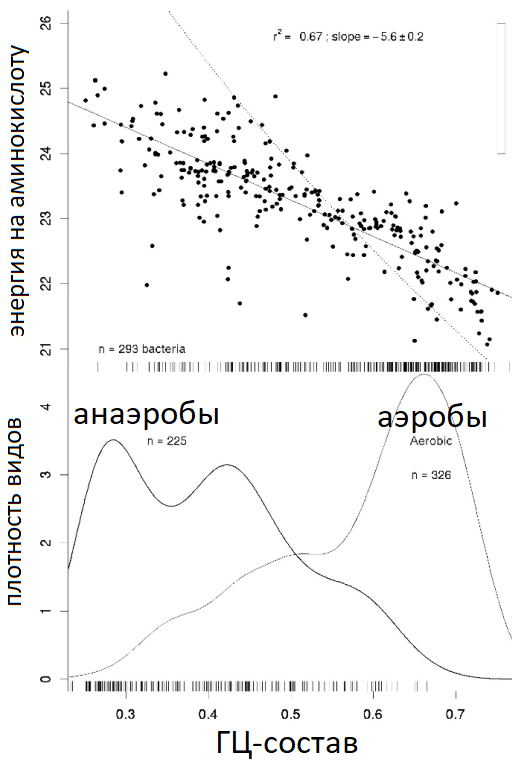
\includegraphics [width=0.5\textwidth] {Dissertation/images/lit/lit1.png}
  \caption{Аэробные бактерии имеют более высокий ГЦ-состав и используют аминокислоты, требующие меньше энергозатрат для синтеза в аэробных условиях. График сверху: зависимость средней энергии, которую нужно затратить на синтез аминокислот представленных в протеоме бактерий, от ГЦ-состава. График снизу: плотность распределения ГЦ-состава у аэробных и анаэробных микроорганизмов. Источник изображения: \cite{lobry2004life}.} 
  \label{img:gc1}  
\end{figure}

Анализ лабораторных экспериментов по накоплению мутаций выявил значительное мутационное смещение в сторону увеличения ГЦ-состава \cite{long2018evolutionary}. Причем оно наблюдалось как в четырежды вырожденных сайтах (все замены являются синонимичными), так и в ноль-вырожденных сайтах (все замены являются несинонимичными), хотя в последних и в значительно меньшей степени. 

\subsection{ГЦ смещение генома}
Неравномерная представленность нуклеотидов в лидирующей и отстающей цепи была обнаружена в 60-х годах двадцатого века \cite{szybalski1966pyrimidine}. Анализ первых трех секвенированных геномов показал, что лидирующая цепь почти равномерно обогащена нуклеотидами Г и Т, в то время как в отстающей чаще встречаются A и Ц \cite{lobry1996asymmetric}. Позднее, данная закономерность, названная ГЦ смещением (GC skew) была выявлена у эубактерий и архей, геномов митохондрий, хлоропластов и вирусов, но не для эукариот со множественными сайтами инициации репликации \cite{lobry1999genomic}. Существуют бактерии без выраженного ГЦ смещения, например, некоторые цианобактерии: \textit{Gloeobacter violaceus} и \textit{Synechococcus elongatus} \cite{arakawa2007gc}. Основную роль в возникновении ГЦ смещения играет, по-видимому, различная мутационная нагрузка на две цепи ДНК, действующая во время репликации. При репликации, лидирующая и отстающая (достраивающейся за счет фрагментов Оказаки) цепи проводят неравное время в одноцепочечном состоянии и в различной степени подвержены дезаминированию, с последующей заменой цитозиновых нуклеотидов на тиминовые. Данные в пользу этого предположения были получены в лабораторных экспериментах по ускоренной эволюции, в которых было показано влияние уровня дезаминирования цитозина (которое, контролировалось в эксперименте) на итоговый уровень ГЦ смещения \cite{kono2018accelerated}. 

\subsection{Chi сайты неравномерно расположены в геноме}
Для сохранения жизни необходима стабильность генома. Для колонизации новых экологических ниш, борьбы с конкурентами, создания более высокоорганизованных организмов, наоборот, нужна динамичность генома - возможность появления и сохранения изменений. Как в обеспечении постоянства генома, так и в его изменчивости, важную роль играет процесс рекомбинации - обмен молекул ДНК своими фрагментами.

Хорошо изучен процесс гомологичной рекомбинации, под которой понимают процесс образования контакта между идентичными или схожими по последовательности фрагментами ДНК с последующим обменом генетическим материалом. Данный процесс позволяет клеткам восстанавливать поврежденные участки ДНК, при условии наличия неповрежденной копии \cite{kuzminov1999recombinational}. Гомологичная рекомбинация также задействована в возобновлении работы остановившихся вилок репликации (например, в следствии недостаточно эффективной работы хеликазы, слишком высокой скрученности ДНК в области репликации, значительного количества белков связанных с ДНК, столкновении репликазы и РНК полимеразы \cite{michel2000resolution, sankar2016nature}.

У прокариот гомологичная рекомбинация играет большую роль в пластичности генома. Именно благодаря этому процессу осуществляются дупликации либо делеции участков ДНК при репликации либо транскрипции, а также замена фрагментов генома на чужеродный материал при горизонтальном перенос генов \cite{ochman2000lateral}. 

В случае, когда в рекомбинации участвуют чужеродные фрагменты ДНК, выделяют два возможных исхода (рисунок~\ref{img:dco_sco}). В одном случае, у двух фрагментов имеются схожие последовательности на краях, и в результате один фрагмент заменяется на другой (рисунок~\ref{img:dco_sco}). Если же привходящая ДНК находится в кольцевой форме и обладает одним схожим по последовательности фрагментом, то происходит вставка без вырезания. 

\begin{figure}[!ht] 
  \center
    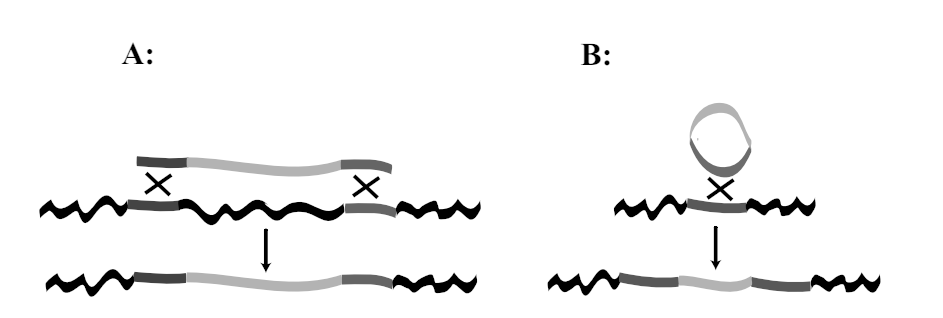
\includegraphics [width=0.75\textwidth] {Dissertation/images/lit/recombination/recombination_dco_sco.png}
    \caption{Варианты рекомбинации при участии чужеродного фрагмента ДНК. Схожие по последовательности фрагменты обозначены темно-серым цветом. А: в случае наличия схожих фрагментов на краях молекул, одна последовательность заменяется на другую; В: в случае, когда привходящая ДНК находится в кольцевой форме и обладает одним участком с высоким сходством последовательности, происходит вставка нового материала без потери исходного варианта. Источник изображения: \cite{mullany2005dynamic}.}
    \label{img:dco_sco}
\end{figure}

У бактерий процесс рекомбинации хорошо изучен на примере кишечной палочки \textit{E. coli}. Важную роль в рекомбинации у данного организма играет комплекс белков RecВCD, обладающий хеликазной, экзо- и эндонуклеазной активностями. Работа этих белков создает ДНК с "липким"\ концом - краевым одноцепочечным фрагментом, что является необходимым условием дальнейших этапов рекомбинации. 

Для образования липких концов необходимо наличие несимметричного разрыва двухцепочечной ДНК. При этом липкие концы образуются на некотором расстоянии от места разрыва. Это расстояние определяется локализацией специфичных последовательностей - Chi сайтов. Данные сайты распознаются белками комплекса RecBCD и, в зависимости от соотношения концентрации АТФ и ионов магния, происходит либо надрез цепи в зоне Chi сайта, либо завершается экзонуклеазная активность RecBCD комплекса (рисунок~\ref{img:rec_chi}) \cite{smith2012recbcd, singleton2004crystal}. В дальнейшем, на одноцепочечном фрагменте происходит кластеризация белка RecA, образование синапса, переброс цепей, образование и разрешение структуры Холидея. 

\begin{figure}[!ht] 
  \center
    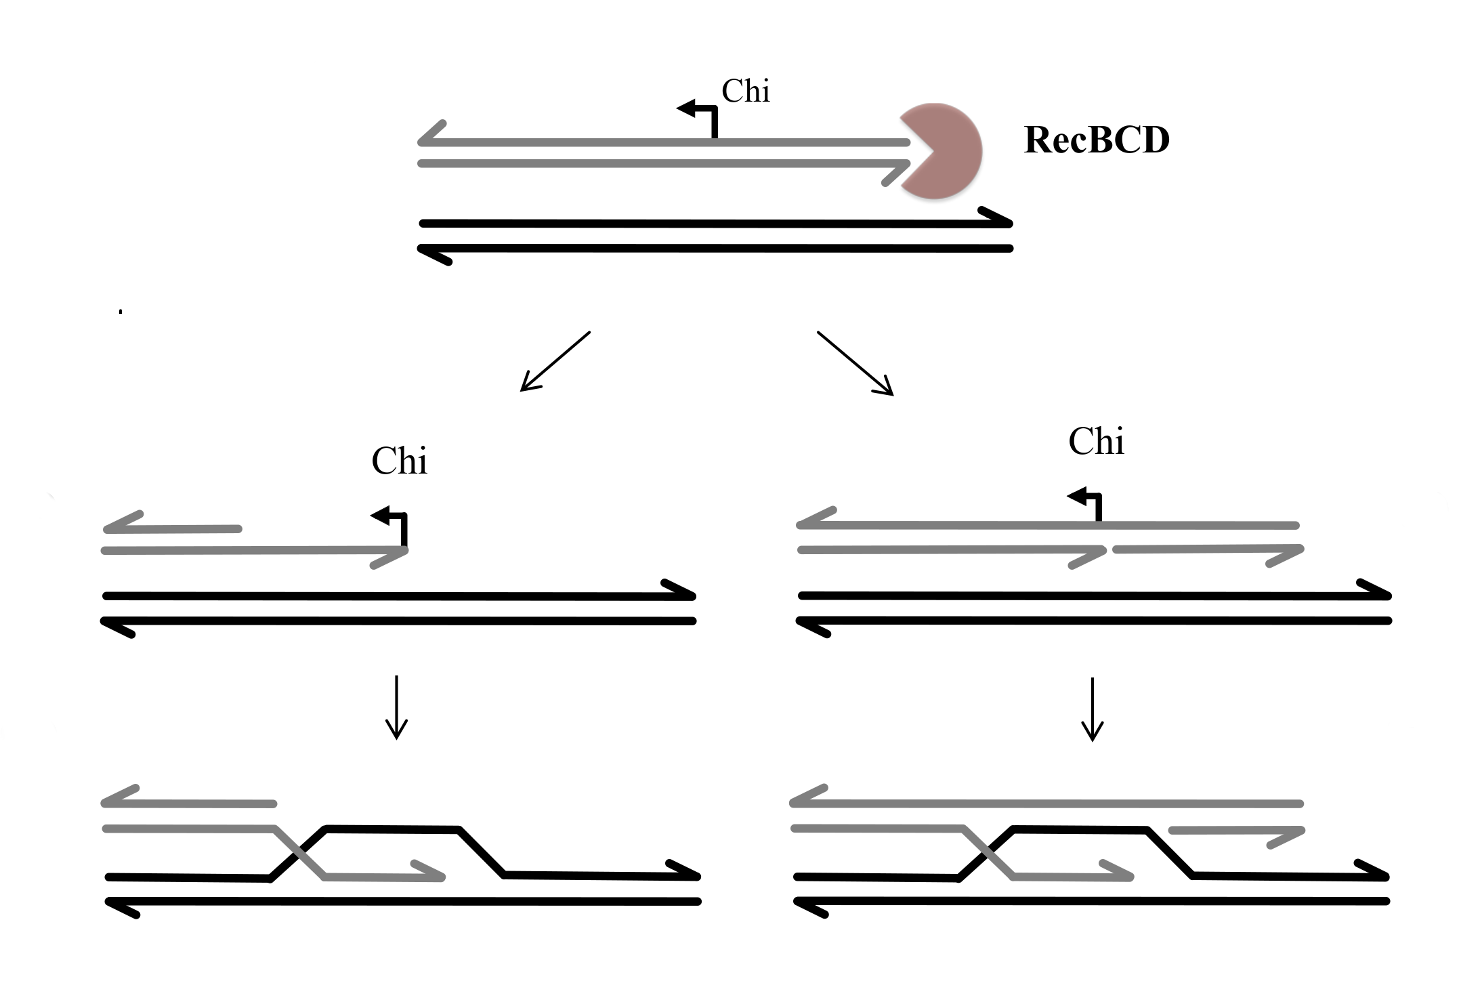
\includegraphics [width=0.85\textwidth] {Dissertation/images/lit/recombination/recombination_chi.png}
    \caption{Участие Chi сайтов в процесса рекомбинации. Данная последовательность распознается белками RecBCD комплекса, что приводит к прекращению продвижения комплекса вдоль цепи ДНК и задает локализацию двухцепочечного разрыва. Источник изображения: \cite{azeroglu2016recg}.}
    \label{img:rec_chi}
\end{figure}

Название сайта Chi является сокращением от crossover hot spot instigator (инициатор горячих точек перекреста). Данные сайты были обнаружены как последовательность, необходимая для осуществления RecBCD зависимой рекомбинации фага лямбда \cite{lam1974rec}. В геноме \textit{E. coli}, находится около тысячи Chi сайтов (примерно по одному на 5 тысяч п.н.) \cite{malone1978hotspots}.

Chi сайты распределены в геноме не равномерно. Они представлены преимущественно в общей для вида части генома, в кор-геноме (core-genome), что вероятно способствует поддержанию его стабильности \cite{halpern2007identification}. В то же время, рибосомные опероны не содержат в себе Chi сайтов (но содержали бы при их случайном расположении) \cite{reams2014recombination}. Наблюдается более редкая встречаемость Chi сайтов в повторяющихся участках генома, что, по-видимому, защищает геном от лишних перестроек, которые бы возникали в случае близкорасположенных повторов \cite{li2019positioning}.

\subsection{Пространственная укладка генетического материала}
У всех организмов ДНК находится в свернутом состоянии, что необходимо для ее размещения внутри клетки (длина хромосомы на несколько порядков превышает длину клетки) \cite{dame2020chromosome}. При этом, пространственная конфигурация молекулы ДНК не случайна, она отражает и регулирует функциональное состояние генома \cite{dekker2008gene}. Так, для эукариот было показано, что петли хроматина, которые размещают промоторы и удаленные энхансеры в непосредственной пространственной близости, играют важную роль в регуляции транскрипции \cite{vernimmen2007long}. У прокариот, укладка хромосомы также, по-видимому, неслучайна и выполняет ряд функций \cite{hofmann2015role}. Подходы, основанные на флуоресцентной микроскопии, позволяют определять субклеточное положение отдельных хромосомных локусов, а высокопроизводительные подходы на основе методов 3C и Hi-C позволяют количественно определять частоты взаимодействия между локусами, которые впоследствии могут использоваться для определения средних трехмерных расстояний между ними. Автоматизация этих методов в начале 2000-х годов позволила проводить исследования пространственной укладки хромосом в масштабе всего генома \cite{umbarger2011three}. 
 
Укладка хромосом у прокариот имеет иерархический характер: от крупномасштабных макродоменов до более мелких структур. Она контролируется при помощи нуклеоид-ассоциированных белков \cite{dame2020chromosome}, одним из которых является гистоноподобный белок H-NS. Он прикрепляется к ДНК преимущественно в локусах с повышенным AT составом и высокой частотой ApT динуклеотида, что характерно для горизонтально перенесенных фрагментов генома \cite{lucchini2006h}. Склонность белка H-NS к образованию цепочек стимулирует образование протяженных нуклеопротеиновых филаментов вдоль одной либо между двух спиралей ДНК \cite{dame2006bacterial}. Считается, что у \textit{E. coli} основными функциями данного белка являются компактизация ДНК и снижение уровня экспрессии горизонтально перенесенных генов \cite{dame2020chromosome}. Множество бактерий имеют гомологи, либо аналоги белка H-NS.

 Другим важным способом поддержания пространственной укладки ДНК являются комплексы структурного поддержания хромосом (structural maintenance of chromosomes, SMC). Эти комплексы способствуют образованию петель ДНК и поддерживают их устойчивость, формируя кольцеобразную структуру вокруг петель \cite{nolivos2014bacterial}. Комплексы SMC также участвуют в сегрегации вновь реплицированных сестринских хромосом \cite{dame2020chromosome}. Мутанты \textit{E. coli} по гену mukB (один из основных белков SMC комплекса у данного организма) имеют нарушенное разделение ДНК по дочерним клеткам и часто производят клетки, лишенные хромосомы \cite{hiraga1989chromosome}. Ряд других белков (IHF, HU, Fis) участвуют в формировании пространственной укладки за счет изгибания ДНК и поддержания её отрицательной суперскрученности \cite{dame2020chromosome}. 

В масштабе от десятков до сотен тысяч оснований, бактериальная хромосома разделена на домены взаимодействия хромосом (chromosome interaction domains, CID), которые аналогичны топологически ассоциированным доменам (topologically associating domains, TAD) у эукариот. ДНК расположена значительно ближе и чаще контактирует внутри доменов, чем между ними (рисунок~\ref{img:chr3d}) \cite{dame2020chromosome}. 

\begin{figure}[!ht] 
  \center
  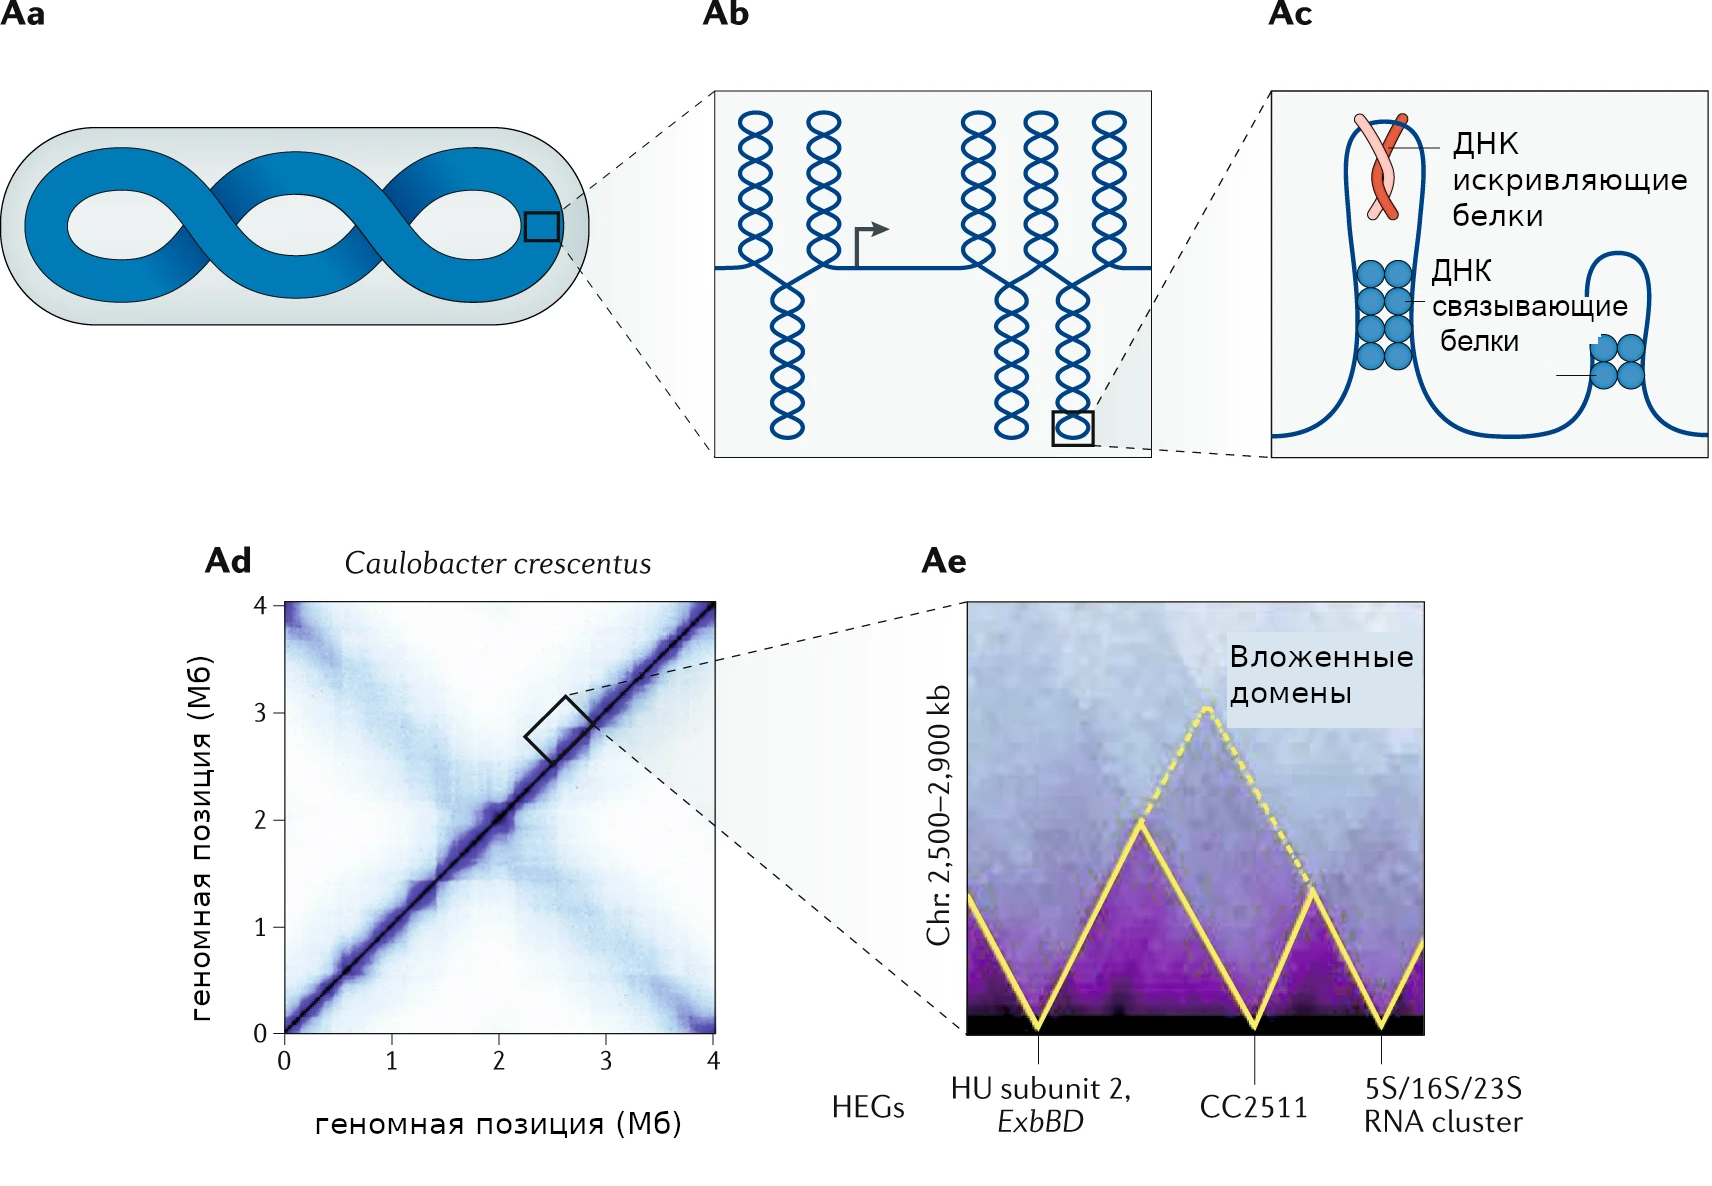
\includegraphics [width=0.9\textwidth] {Dissertation/images/lit/chromosome3d_1.png}
  \caption{Уровни организации пространственной укладки ДНК у прокариот. Пространственная укладка хромосомы многих бактерий имеет форму спирали (Aa), что выражается в наличии двух диагоналей на карте хромосомных контактов (Ad). В масштабе от десятков до сотен тысяч оснований хромосома подразделяется на домены взаимодействия хромосом (Ab). Эти структуры выглядят как квадраты вдоль главной диагонали карты хромосомных контактов (Ad) или как треугольники при наблюдении одной половины симметричной карты(Ae). Домены взаимодействия часто являются вложенными: более крупные домены (прерывистая желтая линия) организованы в более мелкие субдомены (сплошная желтая линия) (Ae). Границы между доменами обычно образованы высокоэкспрессируемыми генами длиной более 2 т.п.н., которые физически разделяют фланкирующий хроматин (часть Ab). Изображение адаптировано из \cite{dame2020chromosome}.} 
  \label{img:chr3d}  
\end{figure}

Количество доменов может зависеть от состояния клетки, так у \textit{Caulobacter crescentus} хромосома организована в 23 домена взаимодействия во время экспоненциального роста в богатой среде и в 29 доменов в условиях голодания; изменение количества доменов вероятно связано с изменением уровня транскрипции генов \cite{dame2020chromosome}. В хромосоме \textit{E. coli} можно выделить 31 домен взаимодействия размером от 40 до 300 тысяч п.н. Двадцать две границы домена соответствуют положениям высоко экспрессируемых генов, а девять границ совпадают с положениями генов, кодирующих белки с сигнальной последовательностью экспорта \cite{lioy2018multiscale}. Выделенное положение генов, кодирующих экспортируемые из клетки белки, может объясняться необходимостью сопряжения процессов транскрипции, трансляции и транслокации \cite{woldringh2002role}. Бактериальные домены взаимодействия имеют вложенный (иерархический) характер, каждый домен состоит из меньших субдоменов (рисунок~\ref{img:chr3d} Ae), самые мелкие единицы этой организации могут соответствовать отдельным оперонам \cite{dame2020chromosome}.

\begin{figure}[!ht] 
  \center
  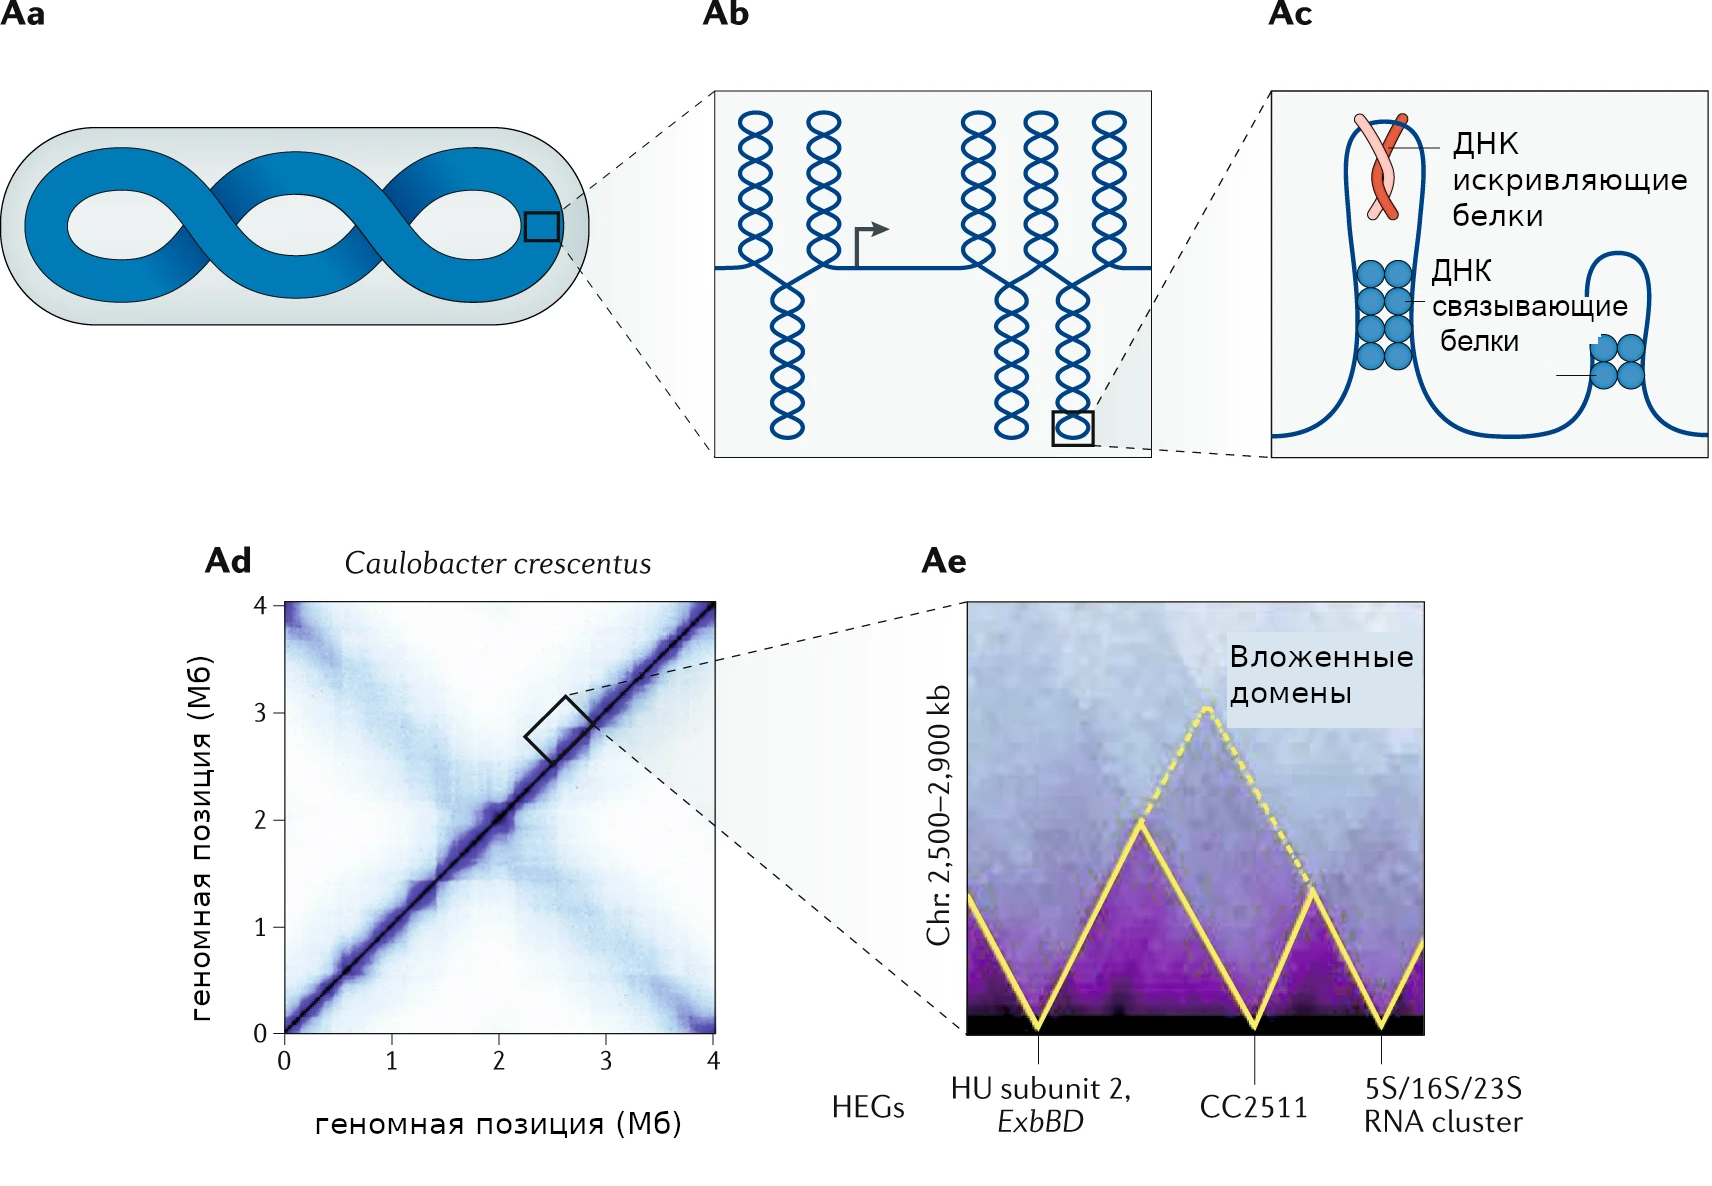
\includegraphics [width=0.9\textwidth] {Dissertation/images/lit/chromosome3d_1.png}
  \caption{Пространственная укладка хромосомы \textit{E. coli}. А) Схематическое изображение пространственной укладки хромосомы \textit{E. coli}, в которой выделяют следующие макродомены: левый (Left), правый (Right), макродомен около сайта начала репликации (Ori) и места окончания репликации (Ter). Б) карта межхромосомных контактов в экспоненциальной фазе роста. В) карта межхромосомных контактов в стационарной фазе роста. Изображение адаптировано из \cite{dame2020chromosome}.} 
  \label{img:coli_3d}  
\end{figure}


Наиболее крупным уровнем пространственной организации прокариотической хромосомы являются макродомены. У \textit{E. coli} хромосома разделена на четыре макродомена и две неструктурированные области (рисунок~\ref{img:coli_3d} ). Все макродомены обладают пониженной подвижность внутри клетки по сравнению с неструктурированными хромосомными участками. Таким образом, макродомены имеют тенденцию взаимодействовать с неструктурированными областями, но не с другими макродоменами \cite{espeli2008dna}. У \textit{E. coli} выделяют макродомен около сайта начала репликации (Ori домен). Ограниченная подвижность Ori домена требует активности белка MaoP (белок макродомена Ori) и мотива из 17 нуклеотидов в вышележащей межгенной области, названной maoS (последовательность макродомена Ori) \cite{valens2016maop}. Механизм, благодаря которому белок MaoP ограничивает подвижность ДНК остается не известен \cite{dame2020chromosome}. Макродомен Ter содержит место окончания репликации, для него описан белок MatP (macrodomain Ter protein), необходимый для существования макродомена (при деактивации данного белка ДНК становится неструктурированной). Белок MatP распознает мотив из 12 нуклеотидов, встречающийся преимущественно в Ter регионе. 

Макродоменная организация хромосомы более выражена во время экспоненциальной фазы роста бактерий. Переход к стационарной фазе связан со снижением уровня доменной организации ДНК, что наблюдается как "размытие"\ квадратов, соответствующих доменам, на карте межхромосомных контактов, получаемой в экспериментах на основе метода HI-C \cite{lioy2018multiscale}.

\section{Горизонтальный перенос генов}
Бактерии и археи размножаются в основном за счет бинарного деления, которому предшествует дупликация генома в родительской клетке. Дочерние клетки получают геном от родительской клетки, что называется вертикальным наследованием. Существует процесс горизонтального переноса генов (ГПГ), при котором клетки приобретают чужеродный генетический материал. На основе анализа геномов было установлено, что горизонтальный перенос часто встречается у прокариот и вероятно сыграл важную роль в их эволюции. Данный процесс позволяет микробам приобретать новые метаболические возможности, занимать новые экологические ниши, приобретать резистентность к воздействию антибиотиков, фагов, атак со стороны эукариот \cite{ochman2000lateral, rodriguez2016flexible, niehus2015migration}. Горизонтальный перенос генов внес наибольший вклад в расширение генных семейств (появления различных вариантов гомологичных белков) \cite{treangen2011horizontal}. В настоящее время интерес к этому процессу во многом продиктован ростом числа резистентных к антибиотикам бактерий, в том числе, бактерий устойчивых ко всем известным антибиотикам \cite{sun2019horizontal}. 

Горизонтальный перенос генов происходит наиболее часто между близкородственными организмами, что объясняется наличием барьеров для переноса между филогенетически-далекими организмами и зачастую низкой функциональностью генов, приобретенных от несхожих организмов \cite{gonzalez2012barriers}. Тем не менее, описаны случаи переноса крупных фрагментов генома между дальнородственными организмами \cite{caro2015inter}. Например, у архей часто находят гены, горизонтально перенесенные от бактерий \cite{wagner2017mechanisms}. В недавней работе, был сделан вывод о происхождении гетеротрофных аэробных архей haloarcheae от архей, являющихся аутотрофными анаэробами, в результате переноса большого фрагмента бактериальной ДНК, содержащей около 1000 генов \cite{wagner2017mechanisms}. Описаны отдельные случаи переноса генов между про- и эукариотами \cite{lacroix2016transfer}. 

Основные способы горизонтального переноса генов у бактерий и архей таковы: трансдукция --- перенос генов при помощи фагов, трансформация --- захват ДНК из окружающей среды, конъюгация --- проникновение ДНК от клетки-донора при контакте с клеткой-реципиентом \cite{thomas2005mechanisms, wagner2017mechanisms}. Описаны и более экзотические способы, при помощи ДНК содержащих мембранных везикул \cite{biller2014bacterial}, передача ДНК при контакте бактерий с помощью синтезируемых ими нанотрубок \cite{dubey2011intercellular}, вирусоподобные агенты горизонтального переноса (virus-like gene transfer agents, GTA) \cite{brimacombe2015homologues}. В большинстве типов переноса, переносимая ДНК должна находиться в одноцепочечной форме, у \textit{E. coli} также описаны механизмы переноса двухцепочечной ДНК \cite{sun2018pull}.

\subsection{Трансформация}
Трансформация --- это процесс захвата и интеграции внеклеточной ДНК характерный для прокариот. Поглощение ДНК требует, чтобы клетка находилась в физиологическом состоянии, известном как компетентность. Для поддержания состояния компетентности требуется активность нескольких десятков (20–50) белков, которые как правило высоко-консервативны \cite{thomas2005mechanisms, sun2018pull}. Интенсивность трансформации зависит от ряда факторов: от концентрации внеклеточной ДНК, от количества соседних компетентных клеток, степени нехватки ресурсов (стресса) \cite{johnston2014bacterial}. 

При трансформации, перемещаемая  ДНК становится одноцепочечной при прохождении через мембрану, и затем может подвергаться гомологичной рекомбинации или использоваться в качестве источника питательных веществ \cite{finkel2001dna}. Интересно, что в то время как белки участвующие в транслокации ДНК обладают высокой консервативностью (почти у всех видов эту функцию выполняют гомологичные белки), пути, регулирующие переключение в состояние компетентности, значительно различаются - у разных видов в этом участвуют различные белки, реагирующие на различные сигналы \cite{johnston2014bacterial}. Это значительно усложняет определение того, является ли некоторый вид естественно-компетентным. Так, \textit{Vibrio cholerae} не считался компетентным до обнаружения роли продуктов распада хитина в индукции состояния компетентности \cite{mell2014natural}. У некоторых видов (например, различных видов \textit{Neisseria} и \textit{Helicobacter}) клетки находятся в компетентном состоянии почти все время жизни \cite{dubnau2019mechanisms}.

Захват ДНК в бактериальных клетках осуществляется при помощи пилей IV типа либо иными подобными структуры \cite{piepenbrink2019dna}. Этот процесс наиболее хорошо изучен у грамм-отрицательных бактерий, в частности у \textit{Vibrio cholerae} и \textit{Neisseria gonorrhoeae}. У данных бактерий после захвата ДНК, пиль сокращается, ДНК проникает внутрь клетки, после чего связывается с периплазматическими белками для предотвращения обратной диффузии, одна цепь ДНК затем переносится через цитоплазматическую мембрану, а другая цепь деградирует \cite{dubnau2019mechanisms}. Подобный механизм, вероятно,
действует и у грамположительных бактерий, но эти системы изучены в меньшей степени \cite{dubnau2019mechanisms}.

\subsection{Мобильные элементы генома}
Горизонтальный перенос генов часто осуществляется при участии мобильных элементов генома. Под мобильными элементами генома понимают фрагменты ДНК, которые способны перемещаться внутри генома или между геномами различных клеток и кодируют все либо часть белков, необходимых для своего перемещения \cite{bellanger2014conjugative}. Наиболее известными и хорошо изученными мобильными элементами являются плазмиды, траспозоны и бактериофаги. Ниже приведено короткое описание этих и некоторых других типов мобильных элементов. 
%https://www.sciencedirect.com/science/article/abs/pii/S1369527416301801

\subsubsection{Плазмиды}
Плазмиды --- это кольцевые или линейные внехромосомные репликоны, которые присутствуют во многих бактериях и археях и встречаются у эукариот \cite{shintani2015genomics}. Они являются одним из основных средств обмена генетической информацией у микробов благодаря способности эффективно перемещаться из одного организма в другой при помощи конъюгации \cite{guglielmini2011repertoire}. 

Длина плазмид находится в диапазоне от единиц до сотен тысяч пар нуклеотидов. Их репликация может осуществляться различными способами. Для кольцевых плазмид характерна тета-репликация, репликация по типу "катящегося кольца", репликация с вытеснением цепи \cite{del1998replication}. На краях линейных плазмид, как правило, присутствуют короткие повторы по функциям схожие с теломерами, которые играют важную роль в репликации данных плазмид \cite{ravin2011n15}.

Конъюгативные плазмиды несут в себе генетически сложные системы для горизонтальной передачи плазмид, включая белки для образования пор спаривания, а также белки репликации и передачи ДНК. Существуют мобилизуемые плазмиды, которые кодируют только часть функций, необходимых для переноса; их горизонтальная передача может происходить только при наличии в клетки других плазмид, несущих недостающие белки. Соотношение подвижных плазмид (коньюгативных и мобилизуемых) к плазмидам, для которых не обнаружены факторы передачи (немобильные), равно примерно 2:1 \cite{redondo2020pathways}. Немобильные плазмиды также могут горизонтально передаваться при помощи процесса трансформации \cite{hulter2017evolutionary}. 

Недавний анализ более чем десяти тысяч плазмид, показал, что для них можно выделить кластеры ("таксономические единицы") с высоким сходством последовательностей внутри кластеров (выше 90\%) и низким, как правило, ниже 70\% сходства в остальных случаях \cite{redondo2020pathways}.

Плазмиды могут встраиваться в хромосому своих хозяев и таким образом обеспечивать изменчивость хромосом \cite{zechner2000conjugative, brunder2000genome}. Такие интеграционные события были обнаружены в геномах \textit{Enterococcus faecalis}, \textit{Shigella flexneri}, \textit{Yersinia pestis}, \textit{E. coli} и ряда других организмов \cite{myers2006role}. 

Встраивание плазмид может сильно влиять на фенотип организма. Для \textit{S. flexneri} и \textit{E. coli} описана плазмида размером 220 т.п.н., встраивание которой в хромосому приводит к тому, что факторы вирулентности, кодируемые данной плазмидой, перестают экспрессироваться и бактерии теряют способность к инвазии. Затем может произойти точное вырезание плазмиды, с восстановлением вирулентности бактерии. Также может происходить неточное (частичное) вырезание, что может приводить к тому, что фрагменты плазмиды остаются в хромосоме \cite{myers2006role}. Описан ретро-транспорт плазмид --- их передача в клетку-рецепиент с последующим возвратом в донорскую клетку. Данный процесс может служить способом приобретения новых генов клеткой-донором, за счет их встраивания в плазмиду, при ее нахождении в клетке-реципиенте \cite{ronchel2000retrotransfer}. Плазмиды обладают высоким уровнем изменчивости и часто содержат в себе различные мобильные элементы. Конъюгативные и мобилизуемые плазмиды таким образом могут служить средством транспорта мобильных элементов генома от одних клеток к другим. Интересной и сравнительно новой темой исследований является взаимосвязь мобильных элементов генома. Так, для холерного вибриона описана мобилизация геномного острова конъюгативной плазмодой \cite{carraro2016inca}. Согласно предложенной модели, мобилизация обеспечивается тем, что на плазмиде кодируется транскрипционный фактор AcaCD, который активирует в том числе и гены, находящиеся в геномных островах, в частности ген фактора направленности рекомбинации xis, продукт которого увеличивает частоту вырезания геномного острова из хромосомы \cite{carraro2017mobilizable}. 

\subsubsection{Интегративные конъюгативные элементы}
Впервые, процесс конъюгации был открыт на плазмидах \cite{lederberg1946gene}. Позднее были обнаружены хромосомные элементы генома способные к вырезанию и конъюгативной передаче --- интегративные конъгативные элементы (ИКЭ)\cite{burrus2002icest1}. Вырезание и интеграция ИКЭ осуществляется за счет интеграз либо транспозаз. На рисунке~\ref{img:ice} показано схематичное изображение структуры и принципа функционирования интегративных конъюгативных элементов. 

\begin{figure}[!ht] 
  \center
  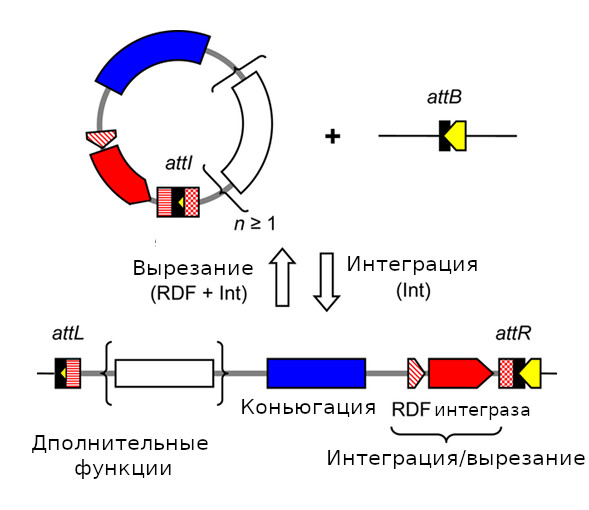
\includegraphics [width=0.7\textwidth] {Dissertation/images/lit/ice.jpg}
  \caption{Устройство и принцип работы интегративных конъюгативных элементов (ИКЭ). Сайт-специфическая интеграция и вырезание катализируются интегразой. RDF является кофактором, необходимым для процесса вырезания (у ряда интеграз). Большие прямоугольники обозначают модули. Тонкие черные линии и толстые серые линии обозначают геном хозяина и ИКЭ, соответственно. Стрелками обозначены гены, а меленькими прямоугольниками - сайты интеграции. Изображение адаптировано из \cite{bellanger2014conjugative}.} 
  \label{img:ice}  
\end{figure}

Разные типы интеграз и транспозаз отличаются сайтами интеграции и уровнем сайт-специфичности. Наиболее хорошо изучены ИКЭ, кодирующие тирозиновые рекомбиназы. Они часто обладают высокой сайт специфичностью, а сайты интеграции широко представлены в генах тРНК и ряде других генов домашнего хозяйства. Описаны также ИКЭ с низкой сайт-специфичностью интеграции. Например, элемент CTnDOT, встречающийся у бактерий рода \textit{Bacteroides} и встраивается в низко-специфичные (но не случайные) сайты \cite{cheng2000integration}. 

Интегративные конъюгативные элементы, наряду с плазмидами, считаются одними из наиболее эффективных способов распространения генов устойчивости к антибиотикам \cite{botelho2020role}. ИКЭ семейства SXT были признаны основными факторами распространения генов устойчивости к антибиотикам среди нескольких видов семейств Enterobacteriaceae и Vibrionaceae, включая экологические и клинические изоляты \textit{V. cholerae} \cite{carraro2015biology}. 

Интегративные конъюгативные элементы значительно отличаются по длине: от десятков т.п.н. (например, элемент pSAM2 у \textit{Streptomyces ambofaciens} \cite{pernodet1984plasmids}) то сотен т.п.н. (у \textit{Streptomyces turgidiscabies} описан элемент PAISt длиной в 674 т.п.н.\cite{kers2005large}). Эта разница в размере в значительной степени зависит от карго-генов, количество которых варьирует от одного гена устойчивости к тетрациклину у Tn916 (одного из наиболее хорошо изученных ИКЭ), до значительного числа генов (в том числе с неизвестными функциями) у PAISt. Состав карго-генов может значительно между близкими ИКЭ, несущими одинаковые либо схожие по последовательности модули конъюгации и рекомбинации. 

\subsubsection{Фаги}
Фаги - вирусы бактерий и архей - являются важным фактором изменчивости геномов своих хозяев \cite{ventura2002transcription}. Первые проекты по секвенированию бактериальных геномов показали значительный вклад профаговых последовательностей в наблюдаемые межштаммовые отличия. Так, в последовательности генома \textit{E. coli O157 Sakai} было идентифицировано 18 профагов (или остатков профагов), они составили примерно половину всех различий в генном составе между данным штаммом и лабораторным \textit{K-12} \cite{hayashi2001complete}. 


Размеры фаговых геномов значительно варьируют, наименьший описанный фаговый геном состоит всего из 2,4 т.п.н., а размеры наиболее длинных геномов превышают 400 т.п.н. Подобно остальным мобильным элементам, фаговые геномы могут нести карго-гены, среди которых встречаются гены патогенности (включая, токсины) \cite{schroven2021bacteriophages}. Так, некоторые фаги семейства лямбда содержат в себе шига-токсин, который является мощным фактором патогенности у шига-продуцирующих \textit {E. coli}; у \textit{Vibrio cholerae} описаны нитчатые фаги CTXf, несущие ген, кодирующий токсин холеры (CTX); известны фаги, наличие которых необходимо для патогенности бактерий \textit{Corynebacterium diphtheriae} и \textit{Clostridium botulinum} \cite{brussow2004phages}. Ряд факторов патогенности присутствует в фагах золотистого стафилококка, сальмонелл, стрептокков \cite{brussow2004phages}. Экспериментально было показано, что некоторые гены вирулентности, содержащиеся в фагах, могут экспрессироваться при нахождении его в виде профага \cite{ventura2002transcription}, ряд других генов (например, шига-токсин фагов семейства лямбда) экспрессируются только когда фаг находится в литической фазе цикла \cite{berger2019carriage}.

Фаги могут участвовать в горизонтальном переносе генов у своих хозяев при помощи процессов специальной и общей (генерализованной) трансдукции \cite{canchaya2003phage, touchon2017embracing}. Умеренные фаги могут встраиваться в геном хозяина - становиться профагами. При последующей индукции, происходит вырезание профага из генома хозяина и наработка вирусных частиц, с последующим их выходом из клетки. Вырезание профага может не совпадать с границами вирусной последовательности и содержать соседние области генома. Тогда части ДНК клетки-хозяина попадут в капсид и будут перенесены в новую клетку, заражаемую фагом. Данный процесс называется специализированной трансдукцией. В соответствии с этой моделью, в ряде геномов в непосредственной близости от сайта интеграции фагов обнаруживаются горизонтально перенесенные гены \cite{canchaya2003phage}. 

Хорошо изучен механизм интеграции у фага лямбда. Интеграза данного фага представляет собой сайт-специфическую тирозиновую рекомбиназу, обеспечивающую рекомбинацию между двумя комплементарными последовательностями ДНК: сайтом attP (250 п.н.), расположенный в геноме фага, и сайте attB (21 п.н.), расположенном внутри бактериального генома \cite{mohaisen2020site}. У многих других фагов, использующих сайт-специфическую рекомбинацию, для успешной интеграции необходимо наличие вспомогательных белков --- факторов интеграции, кодируемых бактериями \cite{mohaisen2020site}. 


Горизонтальный перенос генов может происходить также за счет общей (генерализованной) трансдукции, при которой ДНК хозяина упаковывается в капсид вместо генетического материала фага. После заражения другой клетки, такая ДНК может участвовать в процессе рекомбинации и стать частью генома зараженной клетки. У некоторых бактерий, фаги являются механизмом передачи определенных, неслучайных, фрагментов ДНК. Так, у \textit{Staphylococcus aureus} описан остров патогенности SaPI1 длиной 15 т.п.н., кодирующий токсин Tst участвующий в токсическом шоке. В клетках стафилококка, инфицированных фагом 80a, этот остров вырезается из хромосомы, автономно реплицируется и попадает в капсид собираемых фагов. При проникновении в организм-реципиент, SaPI1 интегрируется с использованием собственных интеграз \cite{ruzin2001molecular}. 

Фаговые геномы обладают высоким уровнем изменчивости, а их отдельные фрагменты часто имеют различную эволюционную историю (мозаицизм) \cite{hatfull2011bacteriophages}. Вероятно, основным фактором такой изменчивости, является незаконная рекомбинация или рекомбинация между короткими консервативными последовательностями; значительный вклад в эти процессы могут вносить фаговые рекомбиназы \cite{hendrix2000origins, hatfull2011bacteriophages}. Особенностью горизонтальной передачи генов при помощи фагов является их устойчивость: фаги могут сохранять свою способность к инфицированию на протяжении многих лет, даже в агрессивной внешней среде, в которой свободная ДНК деградирует. Фаги, как правило, обладают более узким спектром хозяев (по сравнению с плазмидами), что вероятно объясняется их зависимостью от наличия специфических рецепторов на инфицируемых клетках \cite{myers2006role}.
% https://www.sciencedirect.com/science/article/pii/S1369527403000869

\subsubsection{Интегроны}
Интегроны --- это специализированные системы приобретения генов в бактериальных геномах \cite{gillings2014integrons}. Они достаточно широко распространены и встречаются примерно в 10\%-20\% прочитанных геномах \cite{boucher2007integrons, cambray2010integrons}. Как и ряд других мобильных элементов, они могут участвовать в приобретении, экспрессии и распространении генов устойчивости к антибиотикам \cite{gillings2014integrons} и факторов вирулентности \cite{kovach1996putative}. Интегроны могут быть закодированы в хромосоме, либо находиться в составе плазмид и транспозонов \cite{boucher2007integrons}.

\begin{figure}[!ht] 
  \center
  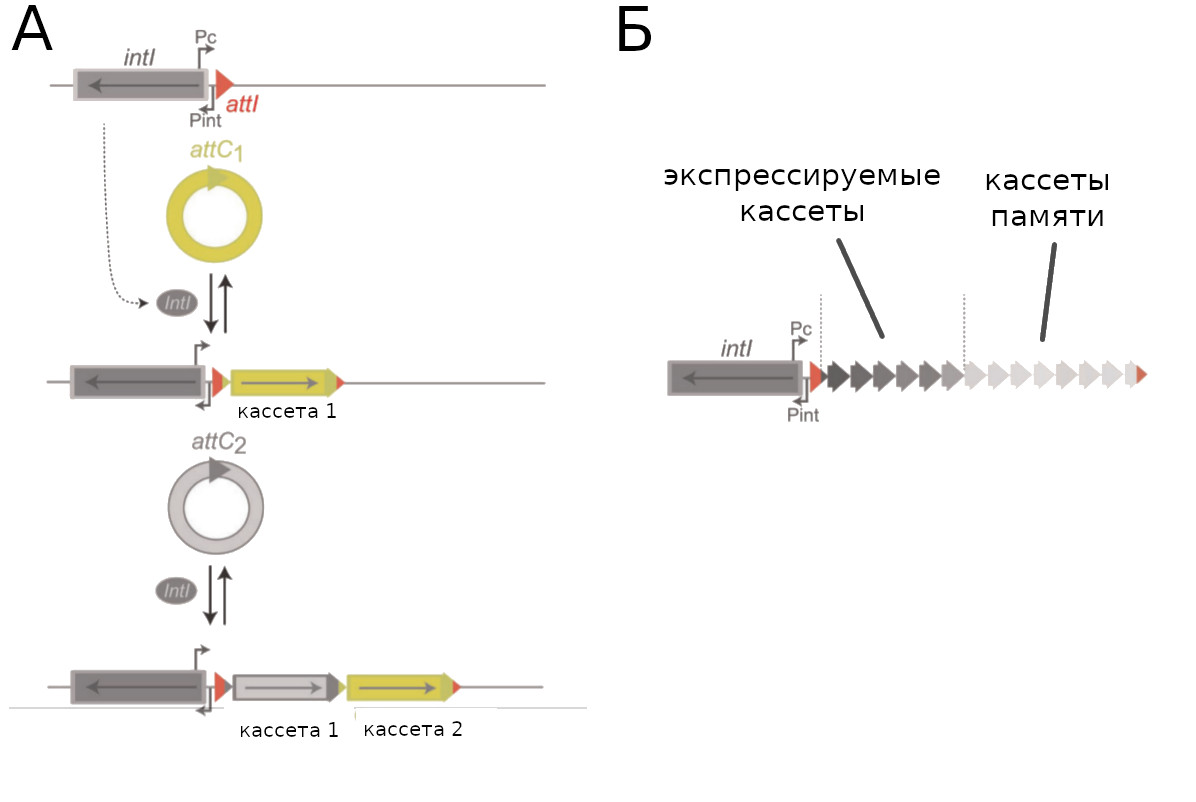
\includegraphics [width=0.85\textwidth] {Dissertation/images/lit/integron.jpg}
  \caption{Устройство и принцип работы оперонов. A) Вставка и вырезание кассет. Интегрон содержит функциональную платформу, состоящую из гена интегразы (intI1), промотора интегразы (Pint), промотора кассеты (Pc) и сайта рекомбинации attI. Б) Уровень экспресии кассет (показан градациями серого цвета) падает по мере удаленности от промотора, только первые из кассет экспрессируются, остальные можно отнести к кассетам ``памяти''. Изображение адаптировано из \cite{boyd2009genomic}.} 
  \label{img:integron}  
\end{figure}

Интегроны содержат ген интегразы (intI), сайт рекомбинации (attI) и промоторные области, необходимые для экспрессии гена интегразы и транскрипции перенесенных в интегрон генов (рисунок~\ref{img:integron}). Эта структура служит платформой для сайт-специфической интеграции нового генетического материала --- генных кассет. Кассеты - кольцевые фрагменты ДНК, как правило состоящие из одного или нескольких генов, лишенных промоторной области. Кассеты также содержат сайт рекомбинации (attC) \cite{gillings2014integrons}. После встраивания, генная кассета становится функциональным геном. Уровень экспрессии встроенных кассет тем выше, чем ближе они расположены к промотору Pc (рисунок~\ref{img:integron}). Интеграза также может случайным образом вырезать генные кассеты и реинтегрировать их на прежнее, либо новое место в интегроне. Таким образом может происходить перестановка генных кассет, с изменение уровня экспрессии встроенных генов. Такая перестановка может служить механизмом подобным простому типу памяти. Кассеты, которые были полезны ранее могут перемещаться в более отдаленные от промотора участки интегрона (например, за счет встраивания новых кассет) что приводит к снижению или прекращению их экспрессии, но не удалению из генома. При последующем возврате к прежним условиям внешней среды, эти кассеты могут подвергнуться процессу перестановки и оказаться вблизи промотора с последующей наработкой с них белков.   

%https://books.google.ru/books?hl=en&lr=&id=oEXzDwAAQBAJ&oi=fnd&pg=PA139&ots=S72ODdX_4B&sig=Qy0nIX9a72y5zxrPvokhgYXw328&redir_esc=y#v=onepage&q&f=false



\subsubsection{Геномные острова}
Понятие геномного острова не определено однозначно. Островами могут называть любые фрагменты ДНК, которые попали в геном в результате горизонтального переноса \cite{langille2010detecting, bazin2020panrgp}. В других работах, под ними понимают такие горизонтально переносимые фрагменты генома, которые содержат в себе "рекомбинационный модуль", включающий в себя интегразу и иные вспомогательные факторы (рисунок~\ref{img:gi}) \cite{boyd2009genomic}. Филогенетический анализ показал, что интегразы, встречающиеся в геномных островах, значительно отличаются от интеграз иных известных мобильных элементов (фагов, интегронов, IS-элементов, интегративных конъюгативных элементов), что может говорить о том, что подобные геномные острова - отдельный вид мобильных элементов генома \cite{boyd2009genomic}. Для ряда геномных островов наблюдалось их вырезание из хромосомы и существование в виде отдельной кольцевой ДНК \cite{blum1994excision, rajanna2003vibrio}. После вырезания, острова могут быть реинтегрированы в хромосому, деградировать либо попасть в новую клетку при помощи общей трансдукции, траснформации либо за счет встраивания в другие мобильные элементы \cite{carpenter2016pathogenicity, pant2020molecular, boyd2009genomic}. На частоту вырезания влияет активность экспрессии рекомбиназ и -- для ряда организмов -- вспомогательных факторов рекомбинации \cite{pant2020molecular}.

\begin{figure}[!ht] 
  \center
  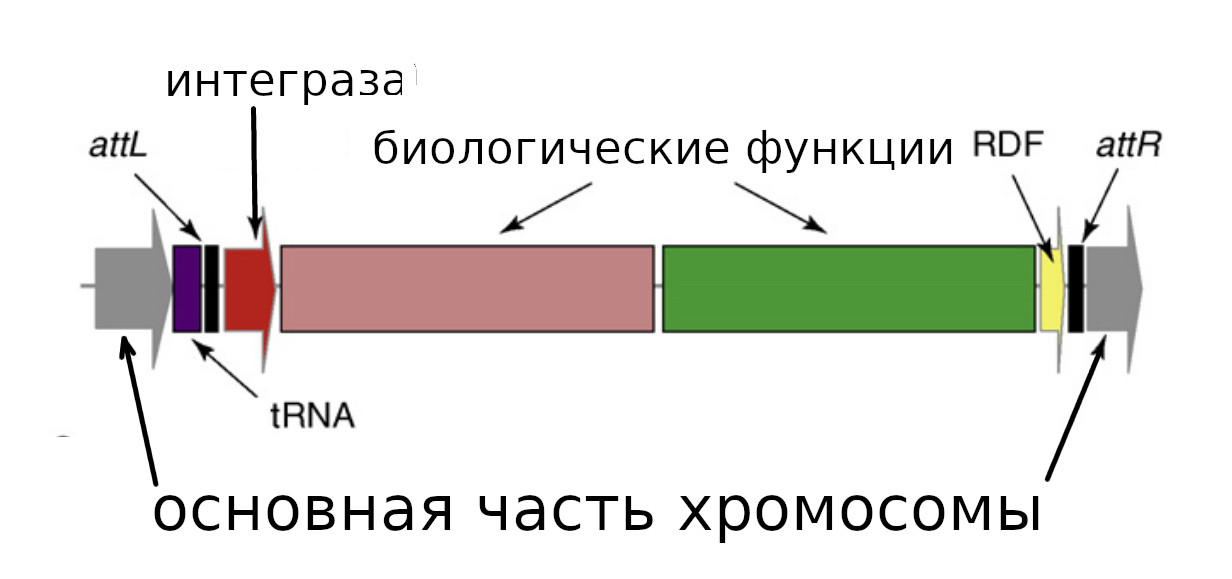
\includegraphics [width=0.7\textwidth] {Dissertation/images/lit/gi.jpg}
  \caption{Схематическое изображение основных компонентов геномного острова. Серые стрелки - основные (коровые) хромосомные гены, фиолетовый прямоугольник представляет - ген тРНК, черные прямоугольники - сайты прикрепления (attL и attR), красная стрелка - ген интегразы, желтая стрелка - фактор направленности рекомбинации (RDF, recombination directionality factor, обнаружены у ряда островов), другие цветные прямоугольники представляют - гены с различными биологическими функциями. Изображение адаптировано из \cite{boyd2009genomic}.} 
  \label{img:gi}  
\end{figure}

Большинство геномных островов, исследованных в работе \cite{boyd2009genomic}, были встроены в гены тРНК, что по мнению авторов обусловлено сайт-специфичностью интеграз и нахождением соответствующих сайтов в генах тРНК. Некоторые геномные острова из рода \textit{Vibrio}, были интегрированы в гены транспортно-матричной РНК (тмРНК). 

Геномные острова отличаются от интегративных конъюгативных элементов тем, что не несут в себе последовательности генов, необходимых для конъюгации, и могут не содержать в своем составе интеграз. Предполагается, что некоторые геномные острова могут передаваться горизонтально за счет использования белков, закодированных в других мобильных элементах (плазмидах, фагах, интегративных конъюгативных элементов) \cite{boyd2009genomic}.

\subsubsection{IS-элементы и транспозоны}
Последовательности вставки или IS-элементы (insertion sequences, IS) являются одними из самых простых мобильных генетических элементов \cite{vandecraen2017impact}. Они представляют из себя короткие (около 1-3 т.п.н.) сегменты ДНК, кодирующие один-два гена и фланкированные инвертированными повторами (рисунок~\ref{img:transposone}А). IS элементы способны к вставке во множество разных мест в. IS-элементы содержат гены транспозазы - белка катализирующего разрезание ДНК и обмен цепями; в некоторых элементах присутствуют регуляторные белки, влияющие на активность транспозазы \cite{siguier2015everyman}. IS-элементы могут перемещаться как внутри генома, так и передаваться между организмами, находясь в составе фагов, плазмид, интегративных конъюгативных элементов \cite{vandecraen2017impact}. Описаны частично деградированные IS-элементы, которые способны к перемещению по геному за счет активности других, интактных, IS-элементов. Такие элементы называются MITE-элементами (miniature inverted repeat transposable elements, MITE) \cite{oggioni1999repeated, siguier2015everyman}. 

IS-элементы играют существенную роль в вариабельности генома \cite{siguier2014bacterial}. Они могут накапливаться в значительном количестве в геноме, а события рекомбинации  между ними часто приводят к удалению геномных фрагментов, что, по-видимому, играет важную роль в уменьшении размера генома видов, перешедших к паразитическому образу жизни \cite{siguier2015everyman}. Встраивание данных элементов в гены, может приводить к потере их функциональности, что в ряде случаев может увеличивать приспособленность организма, например в следствии изменения антигенных детерминант у патогенных микроорганизмов \cite{parkhill2003comparative}. IS-элементы могут увеличивать экспрессию генов за счет образования гибридных промоторов, частично состоящих из фрагментов последовательности IS-элемента \cite{glansdorff1981activation}.

\begin{figure}[!ht] 
  \center
  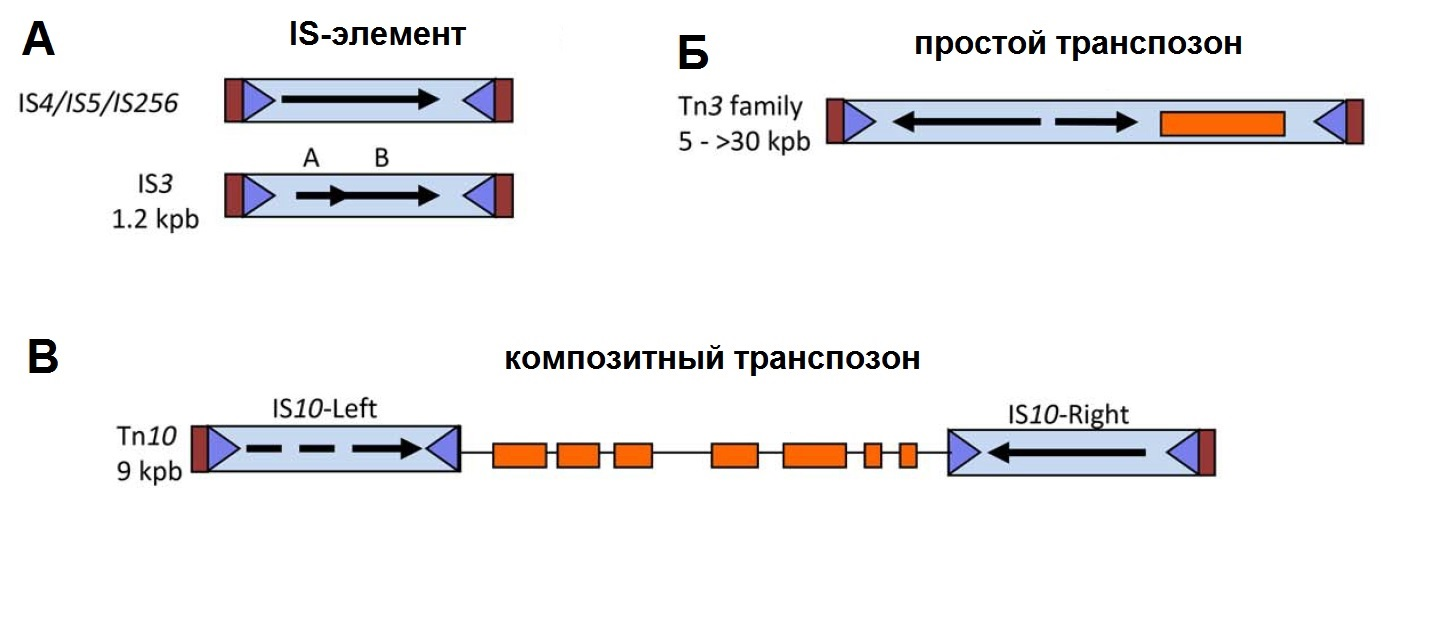
\includegraphics [width=\textwidth] {Dissertation/images/lit/trans.jpg}
  \caption{Схематическое изображение основных типов мобильных элементов, содержащих в себе IS-элементы. IS-элементы показаны голубыми прямоугольниками, концевые инвертированные повторы показаны синими треугольниками, фланкирующие прямые повторы (возникают при интеграции элемента) показаны красными прямоугольниками. Слева указаны семейства IS-элементов и транспозонов, являющиеся их типичными представителями. А) Типичный IS-элемент содержит ген транспозазы и окружен инвертированными и прямыми повторами. Б) Простой транспозон содержит один или несколько генов между повторами. В) Композитный траспозон --- это один или несколько генов, окруженных IS-элементами. Изображение адаптировано из \cite{siguier2015everyman}.} 
  \label{img:transposone}  
\end{figure}

IS элементы могут участвовать в передаче генов, находящихся между ними; такие элементы генома называются составными (композитными или сложными) транспозонами (рисунок~\ref{img:transposone}В) \cite{alton1979nucleotide}. Если IS-элемент содержит в себе один либо несколько карго-генов, то его называют простым транспозоном (рисунок~\ref{img:transposone}Б).  Специфичность встраивания различных транспозонов и IS-элементов значительно различается \cite{wilde2003transposases}.

\subsection{Факторы, влияющие на горизонтальный перенос генов}
Известно, что горизонтальному переносу подвергаются гены всех функциональных категорий, включая и наиболее базовые функции - например, рибосомальные опероны \cite{gogarten2002prokaryotic}. При этом, переноситься могут гены, которые уже присутствуют в геноме реципиента; в таком случае результатом будет не появление нового гена, но замена одно варианта другим. Данный процесс важен для поддержания стабильности генома. Например, для \textit{E. coli} описан сценарий появления склонных к мутациям штаммов за счет поломки генов системы репарации. Затем может происходить исходного уровня мутабельности, за счет горизонтального переноса генов дикого типа \cite{brown2001phylogenetic}. Гипермутабельность может быть полезна в условиях стресса, поскольку может привести к нахождению лучшего в данных условиях варианта генома, а восстановление исходного уровня мутабельности важно для стабилизации нового варианта \cite{caporale2006implicit}.

Для случая переноса новых генов, высказано предположение, что на вероятность того, что ген будет передаваться горизонтально, влияет количество взаимодействий его продукта с другими белками внутри организма \cite{cohen2011complexity}. Согласно данному предположению, чем более тесно связан ген различными взаимодействиями, тем меньше вероятность того, что он будет успешно функционировать в непохожем организме, из-за отсутствия необходимых ему белков-партнеров \cite{novick2020horizontal}.

У ряда естественно-компетентных организмов описаны короткие последовательности (около 12 нуклеотидов), наличие которых увеличивает вероятность горизонтального переноса содержащих их генов. Такие последовательности получили название "последовательности захвата" ("uptake sequences"), поскольку они увеличивают вероятность захвата и переноса ДНК. Подобные последовательности описаны у различных представителей семейств Neisseriaceae и Pasteurellaceae \cite{mell2014natural, spencer2016dna}, вида \textit{Haemophilus influenzae} \cite{smith1995frequency}. Различные виды нейсерий обладают немного различными последовательностями захвата \cite{frye2013dialects}; различия в последовательностях захвата связаны со снижением уровня межвидового переноса ДНК. Чаще всего последовательности захвата представлены в генах "домашнего хозяйства" и кор-геноме в целом \cite{davidsen2004biased}, что подчеркивает важную роль трансформации в поддержании стабильности геномов за счет исправления мутаций при гомологичной рекомбинации \cite{treangen2008impact}.

Геномные перестройки, обусловленные наличием повторов в геноме могут играть регуляторную роль \cite{смирнов2008механизмы}. Так, для кишечной палочки описана инверсия фрагмента генома, окруженного IS-элементами, и дающая выгоды при голодании бактерий \cite {zinser2003bacterial}.

\subsubsection{Области повышенной частоты горизонтального переноса генов}
Области генома с повышенной частотой событий горизонтального переноса генов --- "горячие точки"\ --- были описаны у ряда бактерий \cite{oliveira2017chromosomal}. Они могут возникать за счет сайт-специфичной интеграции мобильных элементов и находиться в генах тРНК, либо иных генах.  У сальмонелл описана область внутри гена ryeA, служившая сайтом интеграции для чужеродной ДНК \cite{balbontin2008insertion}. Многочисленные изменения генного состава наблюдаются в составе геномных островов, для которых описано наличие консервативных и вариабельных фрагментов \cite{vokes1999aerobactin} (механизм вариабельности при этом остается не известным \cite{myers2006role}). Хорошо изученными точками повышенной изменчивости являются интегроны \cite{boucher2007integrons}. 

Наиболее масштабное исследование "горячих точек"\ горизонтального переноса, которое нам известно, было опубликовано в 2017 году, группой Эдуардо Роча \cite{oliveira2017chromosomal}. Авторы провели исследование уровня изменчивости в 80 бактериальных видах; по их оценкам перенесенные гены сконцентрированы только в ~ 1\% хромосомных областей (горячих точек). Они наблюдали, что большинство мобильных элементов генома и генов устойчивости к антибиотикам находятся в "горячих точках"\, но, при этом, во многих высоко изменчивых областях генома мобильные элементы отсутствуют. 

Также в работе \cite{oliveira2017chromosomal} описано наблюдение, что в окрестности "горячих точек"\ генома наблюдается повышенная частота событий гомологичной рекомбинации. По мнению авторов, это объясняется значительной ролью данного процесса в изменении генного состава в высоковариабельных областях генома.

\section{Биоинформатические методы исследования изменчивости генома}
\subsection{Методы поиска ортологии}
Ортологичные гены --- это гены, происходящие от общего предка (гомологи), связанные с общим предком лишь событиями специализации, без участия событий горизонтального переноса либо дупликаций \cite{fitch1970distinguishing}. Определение ортологиченых генов является важным шагом для филогенетического анализа, предсказания функции генов, сравнительных исследований геномов \cite{glover2019advances}. Поиск ортологов вычислительными методами - сложная задача. Для наиболее точного решения требуется реконструкция генного состава предковых геномов и рассчет эволюционных сценариев для каждого гена с реконструкцией событий дупликации, потери и горизонтального переноса генов \cite{glover2019advances}. Помимо значительной вычислительной сложности, полное решение подобной задачи, требует наличия большого количества геномов, которые были бы репрезентативными для исследуемой группы организмов \cite{theissen2002orthology}. Зачастую, задача поиска ортологов решается приближенными методами. 

Наиболее вычислительно простыми являются методы, основанные на оценке сходства последовательностей. К ним относятся, в частности, методы, основанные на поиске лучших двунаправленных совпадений (best bidirectional hit). В основе лежит предположение, что последовательности ортологичных генов более похожи друг на друга, чем на любые другие последовательности в соответствующих геномах \cite{wolf2012tight}. Данный подход был реализован в таких программах как Hieranoid \cite{schreiber2013hieranoid}, ранних версиях и  публичной базы данных OMA \cite{roth2008algorithm}. Данный подход может учитывать только взаимно-однозначные отношения генов. Если в любой из двух сравниваемых линий произошли дупликации генов, для правильного описания потребуется отношение “один ко многим”\ или “многие ко многим”\. В таких случаях подход, основанный на поиске лучших двунаправленных совпадений, упускает из виду многие истинные ортологи \cite{gabaldon2008large, dalquen2013bidirectional}. 

Широкое распространение получила классификация генов по КОГам - кластерам ортологичных групп (Clusters of Orthologous Groups, COG). КОГи рассчитываются на основе поиска троек наилучших совпадений генов и объединении троек, имеющих общие ребра \cite{tatusov1997genomic}; данный подход не столь консервативен как поиск лучших двунаправленных совпадений и не склонен "пропускать"\ гены, ошибочно не соотнося их с их ортологами \cite{derelle2020broccoli}. Конструирование базы COG было произведено с задействованием курирования полученных кластеров человеком, что было возможно во времена, когда количество прочитанных геномов исчислялось десятками \cite{tatusov2000cog}, но не реализуемо в настоящее время с учетом огромного количества прочитанных геномов. Существуют подходы, основаны на кластеризации генов на основе рассчитанных попарных расстояний между ними, в частности, при помощи метода кластеризации на графах MCL (Markov Cluster Algorithm) \cite{li2003orthomcl, emms2015orthofinder}. В отличие от методов, основанных на поиске лучших двунаправленных совпадений, подход MCL является более инклюзивным (меньшее количество генов ошибочно не соотносятся с группами ортологии). В тоже время он может объединять не ортологичные гены в одну группу, за счет сходства последовательностей \cite{derelle2020broccoli}. Примером реализации данного подхода является программа OrthoFinder \cite{emms2015orthofinder}. На вход ей подаются аминокислотные последовательности белок-кодирующих генов во всех рассматриваемых геномах, после чего происходит запуск попарного выравнивания BLAST (опционально можно использовать diamond \cite{buchfink2015fast}), после чего идет этап кластеризация последовательностей при помощи алгоритма кластеризации на графах MCL \cite{vandongen2000cluster}, полученные в результате кластеры называются ортогруппами. В новой реализации данной программы возможен также дополнительный шаг поиска ортологов на основе филогенетического подхода \cite{emms2019orthofinder}.


Существуют методы поиска ортологов, в которых филогенетический анализ является начальным этапом анализа \cite{gabaldon2008large}. Проводимое вручную сравнение филогенетического дерева, построенного на основе выравнивания гомологичных последовательностей, с деревом рассматриваемых видов служило "классическим"\ методом определения эволюционных сценариев; с появлением большого количества прочитанных геномов подобный анализ стал слишком трудозатратным. Были разработаны автоматические алгоритмы сопоставления генного дерева c деревом видов для получения минимального набора событий дупликации и потери генов, позволяющие объяснить наблюдаемые данные \cite{goodman1979fitting}. Это позволило проводить поиск ортологов на основе филогенетического подхода в масштабе полных геномов \cite{wapinski2007automatic}. Основным ограничением ранних реализаций филогенетического подхода является предположение о том, что филогенетические деревья генов и видов не содержат ошибок, что часто не соответствует реальной ситуации, особенно для деревьев отдельных генов в которых уровень филогенетической информации низок и часто присутствуют одинаковые или очень схожие последовательности \cite{rasmussen2007accurate}. Для борьбы с данным недостатком был предложен подход, при котором фрагменты деревьев с низким уровнем достоверности сначала превращались в полиномии (то есть "схлопывались"\ так, что множество ветвей выходило из одного узла) и затем происходило согласование деревьев для гена и для организмов на основе минимизации получаемых событий дупликаций и потери генов \cite{berglund2006optimal}. 


\subsection{Методы поиска горизонтально переносенных генов}
Для выделения горизонтально перенесенных фрагментов генома, используют различные типы методов \cite{sevillya2020detecting}. В первом типе, определяют фрагменты генома, значительно выделяющиеся по некоторой характеристике (сигнатуре) на фоне остального генома. В качестве сигнатуры может выступать ГЦ-состав, индекс использования кодонов, k-мерный спектр (встречаемость комбинаций из k нуклеотидов) \cite{garcia2000horizontal}. Такой подход применялся с начала 1990 годов (например, \cite{medigue1991evidence} и является наиболее простым в вычислительном плане. Особенно эффективен данный метод для определения недавних событий переноса между филогенетически далекими организмами - за счет дальности организмов ожидаемы значительные отличия в сигнатурах, и эти отличия еще не успели затереться из-за процесса "одомашнивания" перенесенного фрагмента ДНК \cite{marri2008gene}. Соответственно, данный тип методов малоприменим для определения переноса между близкими организмами (например, различными штаммами одного вида), поскольку при этом ГЦ состав и иные геномные характеристики ожидаемо будут иметь очень схожие значения. Ограничения данного подхода проистекают также из наличия в геномах вариаций в сигнатурах, не являющихся следствием горизонтального переноса генов \cite{koski2001codon, gogarten2005horizontal}; в частности, отличными от остального генома характеристиками обладают гены мобильных элементов, вирусов и плазмид, а также гены, находящиеся в области конца репликации у ряда бактерий \cite{daubin2003source}. 

Данный тип методов не способен определить донора и реципиента, участвовавших в горизонтальном переносе, задача этих методов --- поиск геномных островов (фрагментов генома, являющихся результатом горизонтального переноса). Примерами реализации данного подхода являются такие программы как Alien hunter \cite{vernikos2006interpolated}, GI hunter \cite{che2014accurate}, GIPSy \cite{soares2016gipsy}. Alien Hunter основан на методе обнаружения атипичных областей в геноме при помощи подхода интерполированных мотивов переменного порядка (IVOM, Interpolated Variable Order Motifs) при анализе содержания G + C, присутствия динуклеотидов и частоте кодонов. Прогнозы оптимизируются с использованием скрытых марковских моделей (HMM) для определения точки входа в атипичные и нетипичные области генома (то есть для уточнения границ горизонтально перенесенного фрагмента). Alien Hunter может делать прогнозы без предварительной аннотации генома. GI hunter тоже основан на методе IVOM, но дополнительно учитывает расположение генов тРНК, наличие интеграз и транспозаз, информацию о генах с высоким уровнем экспрессии, межгенном расстоянии. Все эти данные поступают на вход дерева решений, построенного на обучающей выборке \cite{che2014accurate}. Программа GIPSy также учитывает расположение генов тРНК и генов ассоциированных с мобильными элементами генома, ее отличает функция классификации горизонтально перенесенных фрагментов генома на различные типы: острова патогенности, острова устойчивости к антибиотикам и острова, обеспечивающие симбиоз (symbiotic islands) \cite{soares2016gipsy}. В недавнем сравнении эффективности методов данного типа, наибольшую точность показал Alien Hunter \cite{da2018comparative}.

Второй поход основан на построении филогенетических деревьев отдельно по генам и сравнении их с филогенетическим деревом рассматриваемых организмов (построенном, как правило, на основании общей части геномов (коргенома) либо последовательности 16S рРНК). Гены, для которых эволюционная история плохо совпадает с историей организмов, считаются унаследованными не вертикально (то есть с участием горизонтального переноса либо дубликации) \cite{tofigh2010simultaneous}. Такой подход также начал применяться еще в 1990 годах (например, \cite{smith1992evolution}). Данный подход часто применяется в настоящее время. Например, методом определения горизонтального переноса в базе данных горизонтально-перенесенных генов HGTree \cite{jeong2016hgtree} является метод Ranger-DTL, основанный на филогенетическом подходе \cite{bansal2012efficient}. RANGER-DTL  - это программный пакет для определения эволюции генного семейства с учетом процесса  специализации, дупликации генов, горизонтальному переносу генов и потере генов. Данная программа принимает в качестве входных данных дерево генов и дерево видов и согласовывает их за счет введения предполагаемых событий видообразования, дублирования, передачи и потери генов. Сложность применения данного подхода проистекает от его зависимости от задач, которые сложны и сами по себе - филогенетическая реконструкция и лежащие в ее основе поиск ортологов и множественное выравнивание генов \cite{sevillya2020detecting}. Также, проблему представляет слабость филогенетического сигнала, содержащегося в последовательностях отдельных генов при рассмотрении близкородственных организмов (например, штаммов одного вида). В таком случае деревья, построенные по отдельным генам, содержат много случайных разветвлений с низким уровнем поддержки (например, низкими значениями bootstrap). Для борьбы с возникающими неоднозначностями при реконструкции филогенетического дерева для отдельных генов, в методе GeneRax \cite{morel2020generax} предложено проводить филогенетическую реконструкцию по генам на основе филогенетического дерева для рассматриваемых организмов, за счет этого разрешая возникающие неоднозначности. В качестве входных данных, GeneRax принимает множественное выравнивание для гена и укорененное дерево рассматриваемых организмов (например, построенное на основе общей части геномов). Затем он проводит реконструкцию филогенетического дерева для рассматриваемого гена методом максимального правдоподобия, с учетом различных эволюционных сценариев - событий переноса, дубликации либо потери гена. 

Существуют также программы, реализующие "неявный" филогенетический подход. Например, HGTector основан на сравнении сходств белков рассматриваемого генома по отношению к филогенетически близким и филогенетически более далеким организмам. Ряд методов основаны на поиске отличий в генном составе близкородственных геномов: участки которые есть в определенном геноме и при этом отсутствует в геномах большинства филогенетически близких организмов считаются результатами горизонтального переноса генов. Появляются также гибридные методы, использующие в качестве критериев как различие в сигнатурах, так и филогенетическую информацию \cite{sanchez2020shadowcaster}.

Ожидаемо, разнообразие подходов и методов определения горизонтального переноса приводят к разнообразию в получаемых результатах \cite{ragan2006different}.

\subsection{Методы визуализации отличий в геномах}
В данном разделе мы кратко опишем основные методы визуализации, используемые при сравнении геномов.


Одним из первых способов сравнения последовательностей геномов был метод точечных диаграмм сходства, при котором два сравниваемых генома располагаются по двум осям графика, а точками либо линиями отображаются области сходства между геномами (в англоязычной литературе они получили название dot plot alignment). Пример показан на рисунке~\ref{img:comparison}А. Такой способ применим только для пар геномов и сравнительно редко используется в настоящее время.  

Для сравнения нескольких небольших геномов (например, вирусов) или фрагментов больших геномов применяются графики, в которых отдельными горизонтальными линиями показаны геномы, стрелками обозначены гены, а вертикальные линии соединяют гомологичные гены либо области синтении --- схожих по последовательности участков геномов (рисунок~\ref{img:comparison}Г). Несомненным преимуществом такого способа визуализации является наглядность и удобство прослеживания изменения в расположении отдельных генов; метод применим для небольшого числа сравниваемых геномов (порядка 10-20) и небольшом числе генов. 

Схожим образом, можно показывать множественное выравнивание полных последовательностей геномов бактерий, такие графики часто строят в программе Mauve \cite{darling2004mauve} (рисунок~\ref{img:comparison}Б). Сначала происходит поиск блоков синтении. Блоки синтении отображаются прямоугольниками (как правило, цветными) и соответствующие блоки соединяются линиями. Данный подход также ограничен в применимости сравнительно небольшим количеством геномов (порядка 10), после чего полученные визуализации становятся трудны для восприятия. 

Еще одним подходом к визуализации отличий геномов является представление их на круговой диаграмме (рисунок~\ref{img:comparison}В). При этом, один геном выбирается в качестве референса и отображается на внутреннем круге, остальные геномы располагаются на внешних кругах. Для построения данного типа графиков часто применяется программа BRIG (Blast Ring Image Generator) \cite{alikhan2011blast}; она автоматически производит поиск блоков сходства при помощи алгоритма BLAST и позволяет добавить на график различную метаинформацию (ГЦ-состав, добавленные пользователем аннотированные области). Такой подход позволяет наглядно отобразить области, уникальные для референсного генома (например, геномные острова), но не позволяет показать альтернативные варианты генного состава. Количество сравниваемых геномов может быть достаточно большим (многие десятки) без потери информативности визуализации. 


\begin{figure}[!ht] 
  \center
  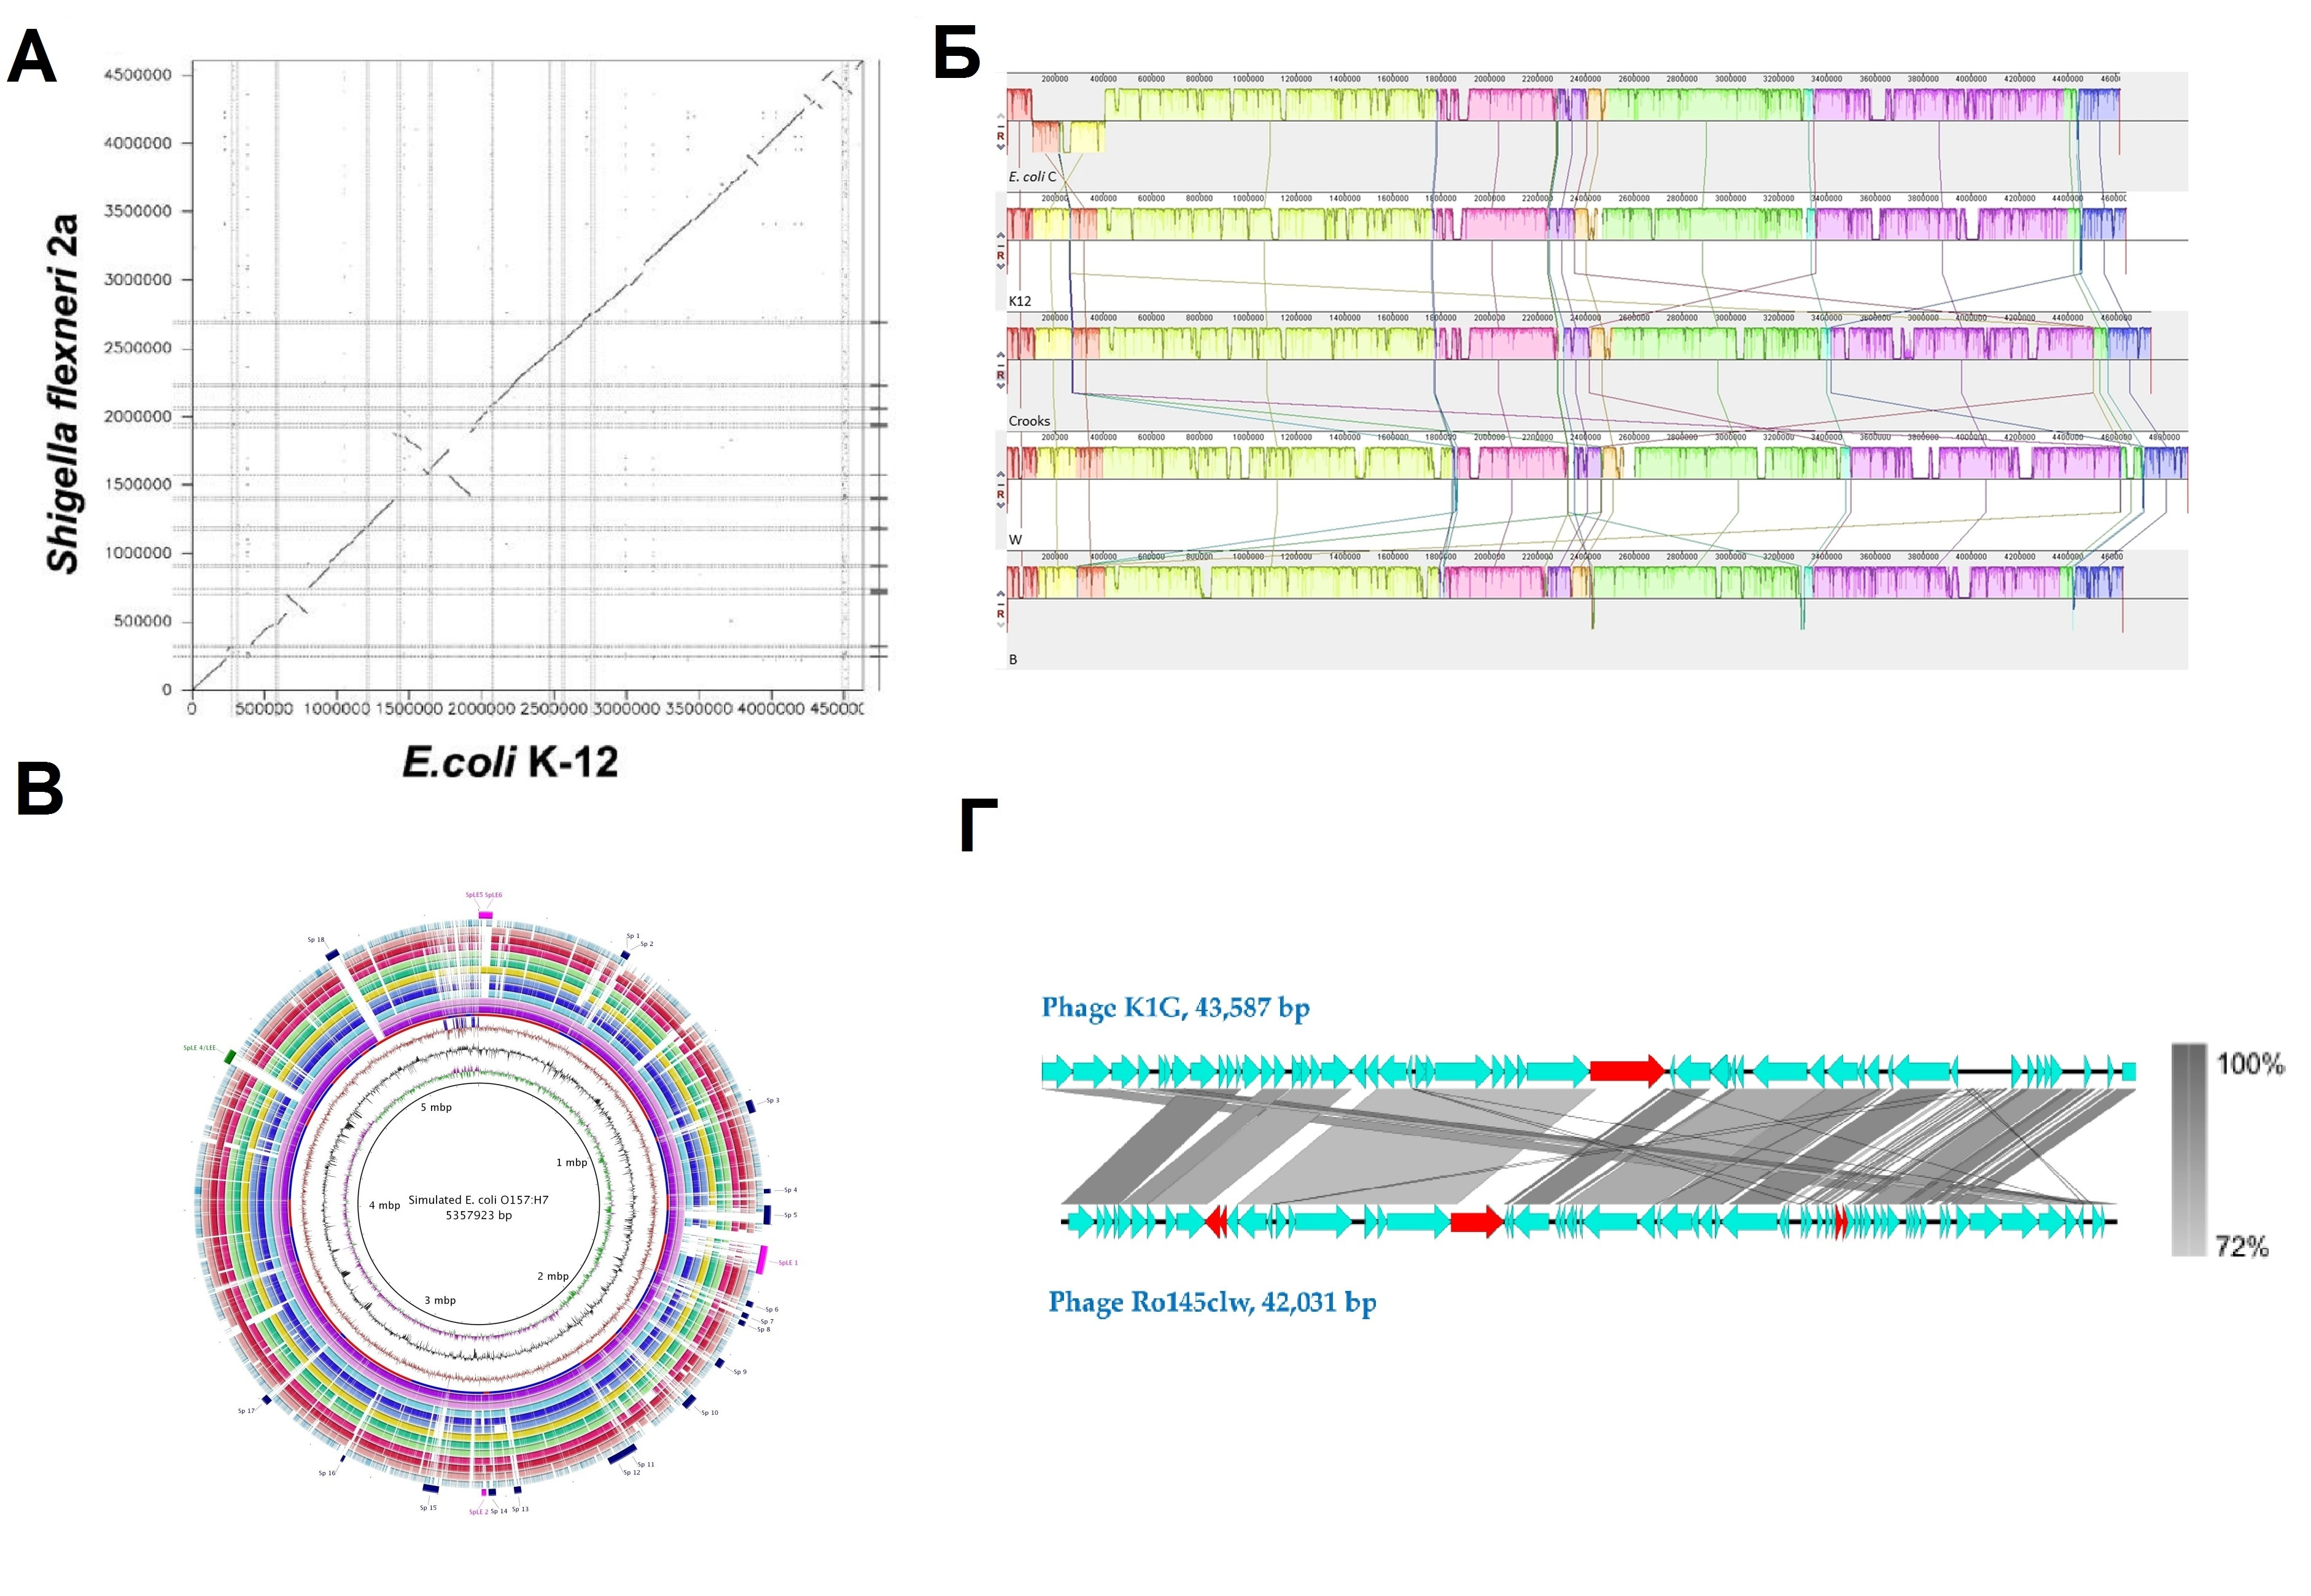
\includegraphics [width=\textwidth] {Dissertation/images/lit/comparisons.jpg}
  \caption{Различые способы визуализации сравнений геномов. А) Сравнение различных штаммов \textit{E. coli}. Координаты геномов сравниваемых штаммов отложены по осям абсцисс и ординат, на пересечении координат ставится точка или проводится линия, при условии совпадения последовательностей по этим координатам. Горизонтальными и вертикальными линиями показано расположение бактериофагов. Изображение адаптировано из \cite{brussow2004phages}, Б) Сравнение различных штаммов \textit{E. coli} при помощи программы Mauve \cite{darling2004mauve}. Показаны крупные блоки синтении; соответствующие блоки соединены линиями. Источник изображения: \cite{krol2019genome}. В) Сравнение геномов различных штаммов \textit{E. coli} при помощи программы BRIG \cite{alikhan2011blast}. Геномы предоставлены в виде колец, внутреннее кольцо соответствует референосному геному. Источник изображения: \cite{alikhan2011blast}. Г) Сравнение состава генов и их расположения в двух фагах. Стрелками обозначены гены, полосами серого цвета показаны схожие последовательности (степень сходства закодирована градиентом серого цвета). Источник изображения: \cite{liao2019characterization}.} 
  \label{img:comparison}  
\end{figure}


\section{Применение графов для анализа геномных данных}

Представление расположения генов в различных геномах в виде графа было применено в работах группы Евгения Кунина в начале 2000х годов \cite{rogozin2002connected, makarova2002dna}. Узлами графа были кластеры ортологичных генов (COG, Clusters of Orthologous Groups of proteins), а ребрами соединялись консервативные пары генов: закодированные на одной цепи, разделенные не более чем двумя генами и представленные в трех и более геномах (из 31 генома, прочтенных к тому моменту).  Целью анализа было нахождение эволюционно устойчивых комбинаций генов. Всего было обнаружено 1505 консервативных пар генов. Большинство пар были представлены лишь в небольшом количестве геномов и только 21 пара генов присутствовала во всех сравниваемых геномах и включала гены рибосомных белков и субъединиц РНК-полимеразы. Также, авторы искали устойчивые кластеры генов, представляющие из себя комбинации устойчивых пар. На рисунке~\ref{img:rogozin_graph} показан граф, представляющий один из обнаруженных кластеров \cite{rogozin2002connected}. Информация об устойчивых кластерах была использована для предсказания функций ранее не охарактеризованных генов архей \cite{makarova2002dna}. В целом, анализ показал, что во многих случаях гены, входящие в кластер, не имели очевидных функциональных связей. По предположению авторов, возможны две альтернативные интерпретации этого результата: 1) гены по соседству только кажутся функционально несвязанными, тогда как в действительности они имеют дополнительные, еще не обнаруженные функции; 2) хотя функциональной связи не существует, продукты этих генов требуются примерно в равных количествах и при тех же условиях, что объясняет преимущество совместного регулирования, обеспечиваемого близким расположением данных генов \cite{rogozin2002connected}. 

\begin{figure}[!ht] 
  \center
  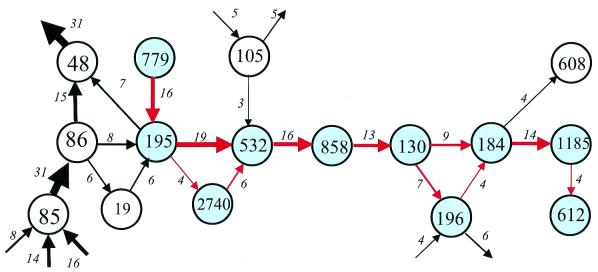
\includegraphics [width=0.8\textwidth] {Dissertation/images/lit/rogozin_graph.jpg}
  \caption{Набор генов, представленный в виде ориентированного графа. Узлы соответствуют кластерам ортологичных генов (COG), номера COG указаны внутри кружков. Иллюстрация взята из работы \cite{rogozin2002connected}. } 
  \label{img:rogozin_graph}  
\end{figure}

% почти граф https://www.ncbi.nlm.nih.gov/pmc/articles/PMC1196056/
В утилите PPanGGOLiN графы, построенные на основе расположения генов (подход, применяемый и в нашей работе), были использованы для классификации генов из пангенома на три категории: устойчивых генов (есть у всех), генов из оболочки (есть у многих) и генов из облака (встречаются у небольшого числа представителей) \cite{gautreau2020ppanggolin}. 
Авторы наблюдали, что доля неконсервативных генов не коррелирует с размером генома.  

Для визуализации графа, который строится в программе PPanGGOLiN, можно использовать графовые редакторы, такие как Gephi (рис~\ref{img:ppangolin}). В декабре 2020 года вышла статья, описывающая модуль программы PPanGGOLiN, предназначенный для поиска геномных островов \cite{bazin2020panrgp}.  

\begin{figure}[!ht] 
  \center
  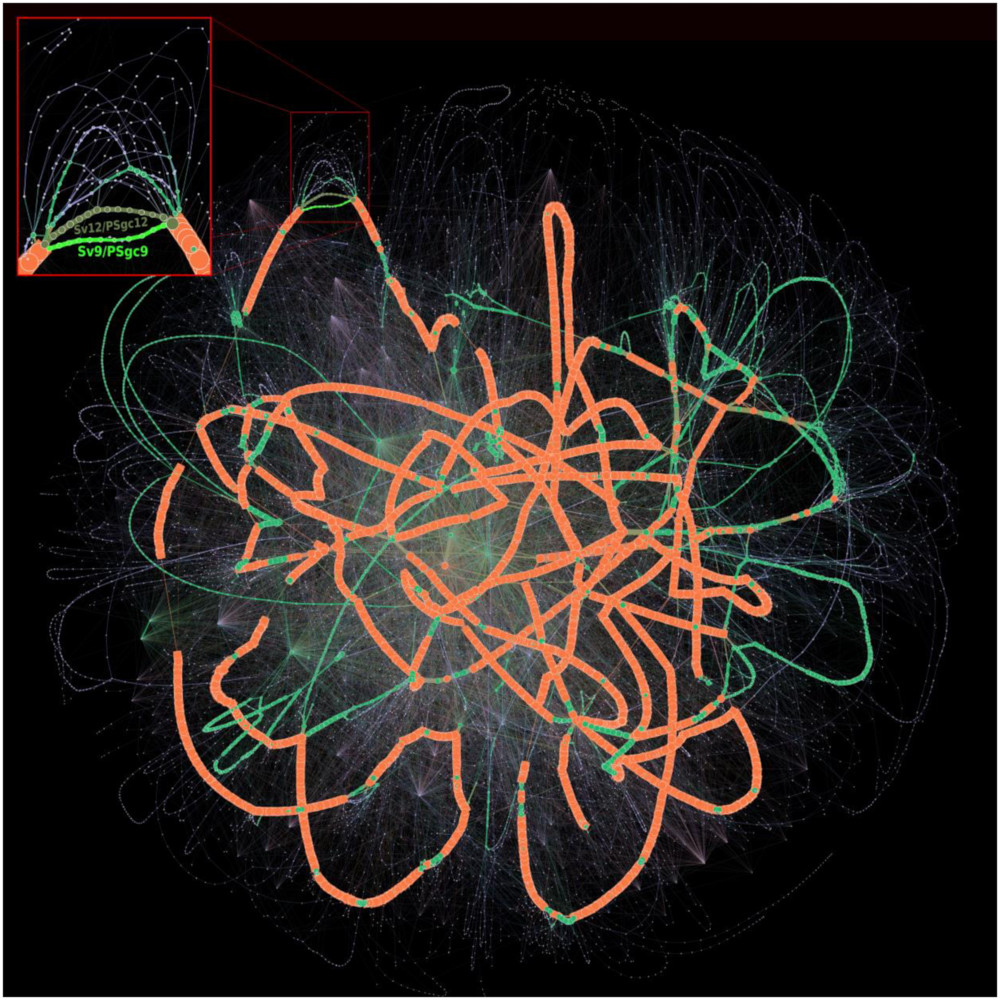
\includegraphics [width=0.6\textwidth] {Dissertation/images/lit/ppangolin.jpg}
  \caption{Пангеномный граф, построенный программой PPanGGOLiN на основе 3117 геномов вида \textit{Acinetobacter baumannii}. Узлы соответствуют семействам генов, ребра соответствуют солокализации генов в геномах. Ребра между генами из устойчивой части генома, оболочки и облака окрашены в оранжевый, зеленый и синий цвета, соответственно. Изображение из публикации \cite{gautreau2020ppanggolin}} 
  \label{img:ppangolin}  
\end{figure}

Также, построение данного типа графов реализовано в пакете FindMyFriends (https://github.com/thomasp85/FindMyFriends) для языка R, предназначенном для проведения пангеномного анализа (поиска групп гомологий, анализа их представленности в геномах). На рис~\ref{img:rfriends} приведен пример визуализации сорасположения генов из различных групп гомологий, выполненный при помощи пакета FindMyFriends.

\begin{figure}[!ht] 
  \center
  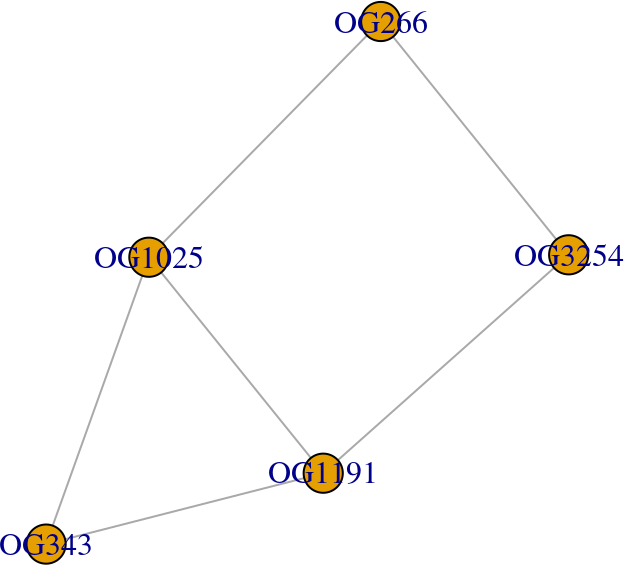
\includegraphics [width=0.5\textwidth] {Dissertation/images/lit/Rfriends.png}
  \caption{Граф сорасположения генов из различных групп гомологий, выполненный при помощи пакета FindMyFriends. Пример из руководства к данному пакету. } 
  \label{img:rfriends}  
\end{figure}


% LDT графы https://arxiv.org/abs/2012.08897

Графы геномной вариабельности, построенные на основе множественного выравнивания, могут быть использованы в качестве референса при картировании прочтений, что улучшает результат картирования (снижает эффект более низкой глубины покрытия в вариабельных участках генома) \cite{paten2011cactus, garrison2018variation}. 

% большой обзор по хромосомной нестабильности https://www.ncbi.nlm.nih.gov/pmc/articles/PMC3957733/

%https://bmcgenomics.biomedcentral.com/articles/10.1186/1471-2164-14-309 -- тут как размывается архитектура в зависимости от филоген. расстояния

\section{Ассоциативная связь болезни Крона с колонизацией \textit{E. coli}}

Болезнь Крона (БК) --- это рецидивирующее воспалительное заболевание кишечника неизвестной этиологии, характеризующееся наличием трансмурального гранулематозного воспаления, диарей, болью в животе, потерей веса, иногда - осложнениями, проявляющихся в иных органах (суставы, печень, глаза) \cite{chervy2020adherent}. Была обнаружена ассоциативная связь между повышенной представленностью \textit{E. coli} в кишечном микробиоме с наличием и тяжестью болезни Крона (как, впрочем, и другими воспалительными заболеваниями кишечника); у пациентов доля кишечной палочки в микробиоте повышена в 10-100 раз (по разным оценкам) по сравнению с ее содержанием у здоровых людей \cite{swidsinski2002mucosal, neut2002changes, miquel2010complete, gevers2014treatment}. Обнаружены мутации в геноме человека, которые увеличивают предрасположенность к болезни Крона. Ряд этих мутаций находится в генах, продукты которых задействованы во взаимодействии человеческого организма и микробиоты  \cite{younis2020inflammatory}. Наиболее вероятным кажется предположение, что в развитии данного заболевания играют роль как факторы внешней среды (включая, нарушение состава микробиоты), так и предрасположенность организма \cite{younis2020inflammatory}. 

Филогенетическое положение изолятов \textit{E. coli} из пациентов с БК значительно варьирует и затрагивает все мажорные филогруппы (A, B1, B2, D) данного организма \cite{rakitina2017genome}. Экспериментально было обнаружено, что ряд изолятов кишечных палочек, полученных от пациентов с БК, оказались способными проникать в эпителиальные клетки кишечника и выживать в макрофагах, что было названо адгезивно-инвазивным фенотипом \cite{boudeau1999invasive, martinez2009molecular,  miquel2010complete}. Согласно мета-анализу, проведенному в 2020 году, кишечная палочка с адгезивно-инвазивным фенотипом встречается у 29\% пациентов с болезнью Крона, что значимо чаще, чем у здоровых людей (у них она встречается в 9\% случаев) \cite{nadalian2020prevalence}. Установить с определенностью генетические детерминанты, позволяющие бактериям приобретать адгезивно-инвазивный фенотип, не удается \cite{shaler2019unique, camprubi2018comparative}. Среди генов, чаще встречающихся у изолятов кишечной палочки из пациентов, по сравнению с изолятами из здоровых людей, в нашем и других исследованиях, были определены гены оперона утилизации 1,2-пропандиола \cite{rakitina2017genome, viladomiu2021adherent, dogan2014inflammation}. Данное вещество является продуктом переработки фукозы комменсальными микробами. У сальмонелл (филогенетически близких к кишечным палочкам патогенных микроорганизмов), утилизация 1,2-пропандиола происходит наиболее эффективно в условиях протекания в кишечнике воспалительной реакции, поскольку при воспалении в просвет выделяются вещества, которые сальмонелла использует как акцепторы электронов. При этом, она становится бенефициаром патологического процесса, а значительная часть иной микрофлоры погибает \cite{faber2017respiration}. Схожий сценарий можно предположить и для кишечной палочки. Вероятно, для нее выгодно провоцировать воспалительную реакции, поскольку это позволяет эффективно утилизировать доступный источник питания и получать доминирующее положение в микробиоме \cite{rakitina2017genome}. Оперон утилизации пропандиола представлен у филогенетически далеких организмов и часто рассматривается как продукт горизонтального переноса генов \cite{anast2020cobalamin, bobik1997propanediol}.

К другим генам кишечных палочек ассоциированными с наличием у их носителя болезни Крона, в разных работах относят гены, вовлеченные в захват железа \cite{rakitina2017genome, nash2010genome}, синтез капсулы \cite{rakitina2017genome, conte2014adherent}, синтез пилей первого типа \cite{cespedes2017genetic}, ген кодирующий белок внешней мембраны OmpC \cite{rolhion2007ompc} и ряд других.


         
\subsection{Отбор последовательностей геномов}
Для анализа геномной изменчивости \textit{E. coli} мы использовали 327 геномов данного организма доступные в базе RefSeq на момент ноября 2017 года и собранных до уровня репликонов ("финишированная"\ сборка). Для анализа изменчивости в различных филогруппах \textit{E. coli} нами были отобраны пять геномов от представителей наиболее крупных филогрупп (подбор проводился на основе литературных данных). Затем для каждого представителя были выбраны 100 наиболее близких по геномов, доступных в базе RefSeq. В качестве меры сходства последовательностей мы использовали суммарную ширину выравниваненных фрагментов генома, выравнивание проводилось программой nucmer \cite{marccais2018mummer4}. 

Для анализа внутривидовых структур у \textit{Pseudomonas aeruginosa}, \textit{Pseudomonas fluorescens} и \textit{Neisseria gonorrhoeae} нами были выгружены все полногеномные последовательности, доступные в RefSeq. Для каждого вида в отдельности было построено филогенетическое дерево при помощи утилиты ParSNP v1.2 \cite{treangen2014harvest}. На основании полученных филогенетических деревьев мы выбрали (визуальным анализом, основываясь на количестве геномов и изолированности от иных клад) от двух до четырех клад дерева. 

Для анализа других видов прокариот мы собрали набор последовательностей геномов всех видов, для которых было доступно не менее 50 последовательностей геномов в базе данных RefSeq. При наличии более 100 последовательностей геномов, в анализ включались 100 случайно выбранных последовательностей. Таким образом была сформирована выборка из 143 видов прокариот, включая два вида архей.

\subsection{Анализ геномной вариабельности}
Белок-кодирующие последовательности во всех загруженных геномах были аннотированы с помощью программы Prokka ver 1.11 \cite{seemann2014prokka}. Гены были отнесены к ортогруппам с помощью OrthoFinder ver. 2.2.6 \cite{emms2015orthofinder}. Скрипты на языке Python, содержащиеся в приложении GCB (https://gcb.rcpcm.org/), использовались для оценки уровня изменчивости генома и создания подграфов вокруг интересующих областей генома. Принципы их работы описаны в соответствующих разделах главы Результаты. Визуализация подграфов проводилась в программе Cytoscape \cite{smoot2011cytoscape}. Для формализации определения областей генома с повышенной изменчивостью мы использовали критерий Тьюки, основанный на межквартильном расстоянии.


Статистическая обработка и визуализация данных мы проводили на языке R. Для определения коэффициентов корреляции Спирмена использовали функцию \textit{cor}. Статистическая значимость корреляций определялась при помощи функции \textit{cor.test}. Индексы согласованности признаков с филогенетическим деревом (retention index) рассчитывались с использованием функции RI из библиотеки phangorn для языка R. Для построения линейных моделей использовалась функция \textit{lm} языка R.

Для построения филогенетического дерева различных видов рода \textit{Bacillus} мы выровняли транслированные последовательности всех ортологичных однокопийных генов при помощи программы muscle \cite{edgar2004muscle}, преобразовали их в выравнивания кодонов с помощью pal2nal и построили дерево с помощью iqtree v1.6 \cite{nguyen2015iq} с опцией ModelFinder Plus (оптимальный подбор эволюционной модели); конвейер snakemake для этих шагов доступен по адресу https://github.com/paraslonic/orthosnake/blob/tree/Snakefile\_tree. 

Поиск областей синтении мы проводили с помощью программы nucmer \cite{marccais2018mummer4}(при сравнении последовательностей геномов различных штаммов одного вида), либо программы Mauve \cite{darling2004mauve} (при сравнении последовательностей геномов принадлежащих различным видам).

Для определения профагов в геномах мы использовали онлайн сервис Phaster \cite{arndt2016phaster}. 

Для \textit{E. coli} мы использовали нормированную матрицу контактов из работы \cite{lioy2018multiscale} и доступную в репозитории: \url{https://github.com/koszullab/E_coli_analysis/tree/master/data}. Для \textit{B. subtilis} мы использовали матрицу контактов из статьи \cite{marbouty2015condensin}. Для нормировки матрицы хромосомных контактов использовалась функция  \textit{normalizeCore.performIterativeCorrection} из библиотеки gcMapExplorer \url{https://github.com/rjdkmr/gcMapExplorer}, количество итераций равнялось 1000, значение шага составило 0.00001. Для построения линейных моделей использовалась функция \textit{lm} языка R.

\section{Сборка и анализ геномов \textit{E. coli} от пациентов с болезнью Крона}

\subsection{Группа пациентов и клинический материал}
Пациенты были отобраны из двух клинических центров (ЦНИИ гастроэнтерологии и Государственного научного центра колопроктологии) в Москве, Российская Федерация, с 2012 по 2014 год. В исследование были включены десять пациентов. Критерии включения были следующими: возраст старше 18 лет, болезнь Крона была диагностирована эндоскопически и гистологически подтверждена. Критериями исключения были признаки неопределенного колита, инфекционные заболевания, недавнее лечение антибиотиками. 
Для исследования были собраны три типа образцов: 1) образцы кала; 2) биопсийный материал, полученный в ходе эндоскопического исследования; 3) жидкое содержимое подвздошной кишки.

\subsection{Выделение изолятов \textit{E. coli}}

Выделение \textit{E. coli} выполняли следующим образом. Приблизительно 0,05 мл объема фекалий помещали в 0,5 мл стерильного буфера (PBS), перемешивали на вортексе до гомогенности, аликвоту разбавляли примерно в $10^6$ раз. Затем 0,1 мл полученной жидкости наносили на чашки со средой LB. После инкубации в течение ночи при 37$^\circ$C изолированные колонии идентифицировали с помощью программного обеспечения Matrix Assisted Laser Desorbtion / Ionization (MALDI) Biotyper (Bruker Daltonics, Германия) с использованием масс-спектрометра Microflex LT (Bruker Daltonics, Германия). Для экстракции ДНК все штаммы \textit{E. coli} выращивали в бульоне LB при 37$^\circ$C при встряхивании (200 об/мин) в течение ночи и собирали центрифугированием.

\subsection{Экстракция ДНК и геномное секвенирование}

Геномную ДНК из отдельных культур экстрагировали с помощью набора QIAamp DNA Mini (Qiagen) в соответствии с протоколом производителя. Экстрагированная ДНК (100 нг для каждого образца) была разрушена на фрагменты размером 200 – 300 пар нуклеотидов с помощью системы Covaris S220 (Covaris, Woburn, Massachusetts, USA). Эмульсию ПЦР проводили с помощью набора Ion PGM Template OT2 200 (Life Technologies). Секвенирование ДНК выполняли с помощью Ion Torrent PGM (Life Technologies) с чипом Ion 318 и набором Ion PGM Sequencing 200 v2 (Life Technologies). 

Всего было получено 28 геномных последовательностей \textit{E. coli} от 10 пациентов с болезнью Крона.

\subsection{Сборка генома, исправление ошибок в гомополимерных областях}
Последовательности генома были собраны с использованием программ Mira 4.0 \cite{chevreux1999genome} со стандартными параметрами и SPADES 3.10.0 \cite{bankevich2012spades}.

Каждая сборка проверялась на наличие возможных контаминаций (последовательностей нецелевого организма) при помощи скрипта, написанного на языке R и доступного по адресу: \url{https://github.com/paraslonic/BacPortrait/blob/master/portrait\_spades.r}. Данный скрипт отображает каждый контиг (отдельный фрагмент сборки) на диаграмме с ГЦ-составом и глубиной покрытия контига; дополнительно отображается информация о таксономической аннотации заданного числа контигов. 
 
Для технологии секвенирования Ion Torrent характерно наличие значительного количества ошибок в определении копийности нуклеотидов, особенно в гомополимерных областях. Для исправления данного типа ошибок, которые могут приводить к ошибкам сборки и искусственному сдвигу рамки считывания в кодирующих последовательностях (CDS), нами был разработан следующий метод. Проводилось картирование прочтений на сборку; поиск позиций с вставками либо делециями в картированных прочтениях при помощи утилиты VarScan; выравнивание областей сборки вокруг найденных позиций при помощи программы BLAST на базу nt (NCBI); выбор варианта последовательности, который соответствует лучшему выравниванию BLAST и представлен в прочтениях с частотой не ниже 25\%. Этот метод уменьшает количество артефактных мутаций в сборке примерно в 2,5 раза (оценка основана на сравнении сборок считываний Ion Torrent до и после исправления с считываниями более точных технологий секвенирования, таких как Illumina, SOLID и Sanger). Вычислительный конвейер для данной процедуры доступен по адресу: \url{www.github.com/paraslonic/HomoHomo}.

Последовательности геномов доступны в GenBank со следующими номерами доступа: RCE01 (JUDV00000000), RCE02 (JUDW00000000), RCE03 (JUDX00000000), RCE04 (JUDY00000000), RCE05 (JWJZ00000000), RCE06 (JWKA00000000), RKA00000000 (JWKA00000000), RKA000006 (JWKA00000000), RKA00000000 JWKB00000000), RCE08 (LAXB00000000), RCE10 (LAXA00000000), RCE11 (LAWZ00000000).

\subsection{Сбор внешних данных}
Для проведения анализа по поиску оперонов, чаще встречающихся в кишечных палочках, изолированных от пациентов с болезнью Крона по сравнению с изолятами, полученными от здоровых людей, мы также использовали внешние данные, собранные на основании анализа литературы. Геномы \textit{E. coli} изолированные от пациентов с болезнью Крона были взяты из работ \cite{nash2010genome, miquel2010complete, krause2011complete}. В группу контроля входили геномы, описанные как комменсальные или лабораторно культивируемые непатогенные штаммы (полный список доступен в публикации \cite{rakitina2017genome}).

\subsection{Поиск ортогрупп}
Полученные последовательности генома аннотировали с помощью программы PROKKA 1.7 \cite{seemann2014prokka}. Информация об оперонной структуре была получена из базы данных DOOR \cite{mao2014door}. Ортогруппы (группы гомологий включающие как ортологичные, так и паралогичные гены) были получены с помощью программы OrthoFinder v1.0.8 \cite{emms2015orthofinder} с параметрами по умолчанию. 

Статистический анализ представленности генов и оперонов в последовательностях генома комменсальных штаммов \textit{E. coli}, либо штаммов, полученных от пациентов с болезнью Крона, проводился при помощи скриптов на языке R, принцип работы которых описан ниже.
         
% ################################################################### Complexity1
\chapter{Результаты}
\section{Разработка и верификация метода оценки изменчивости генома на основе графового представления расположения генов} \label{chaptComplex1}

\subsection{Разработка способа представления расположения генов в виде графа}
Рассмотрим три условные генома, показанные в верхней части рисунка~\ref{img:graph_scheme}. Предположим, что мы установили группы гомологии и стрелками одного цвета показаны гомологичные гены. Для представления этого набора геномов в виде графа, будем ставить в соответствие каждому множеству гомологичных генов узел графа. Ребрами соединим узлы, для которых гены из соответствующих групп гомологии расположены последовательно хотя бы в одном геноме. Вес ребра установим в количество геномов, подтверждающих данную связь (в этих геномах соответствующие гены расположены последовательно). Таким образом мы закодировали информацию о расположении генов в наборе геномов в виде графа (нижняя часть рисунка~\ref{img:graph_scheme}). 

В рассмотренном примере, мы представили  три генома, содержащих суммарно 21 ген, в виде графа из 10 узлов. Чем большее количество геномов будет использовано в анализе, тем выше будет "экономия"\ --- разница между количеством генов и количеством узлов в построенном графе.

\begin{figure}[!ht] 
  \center
    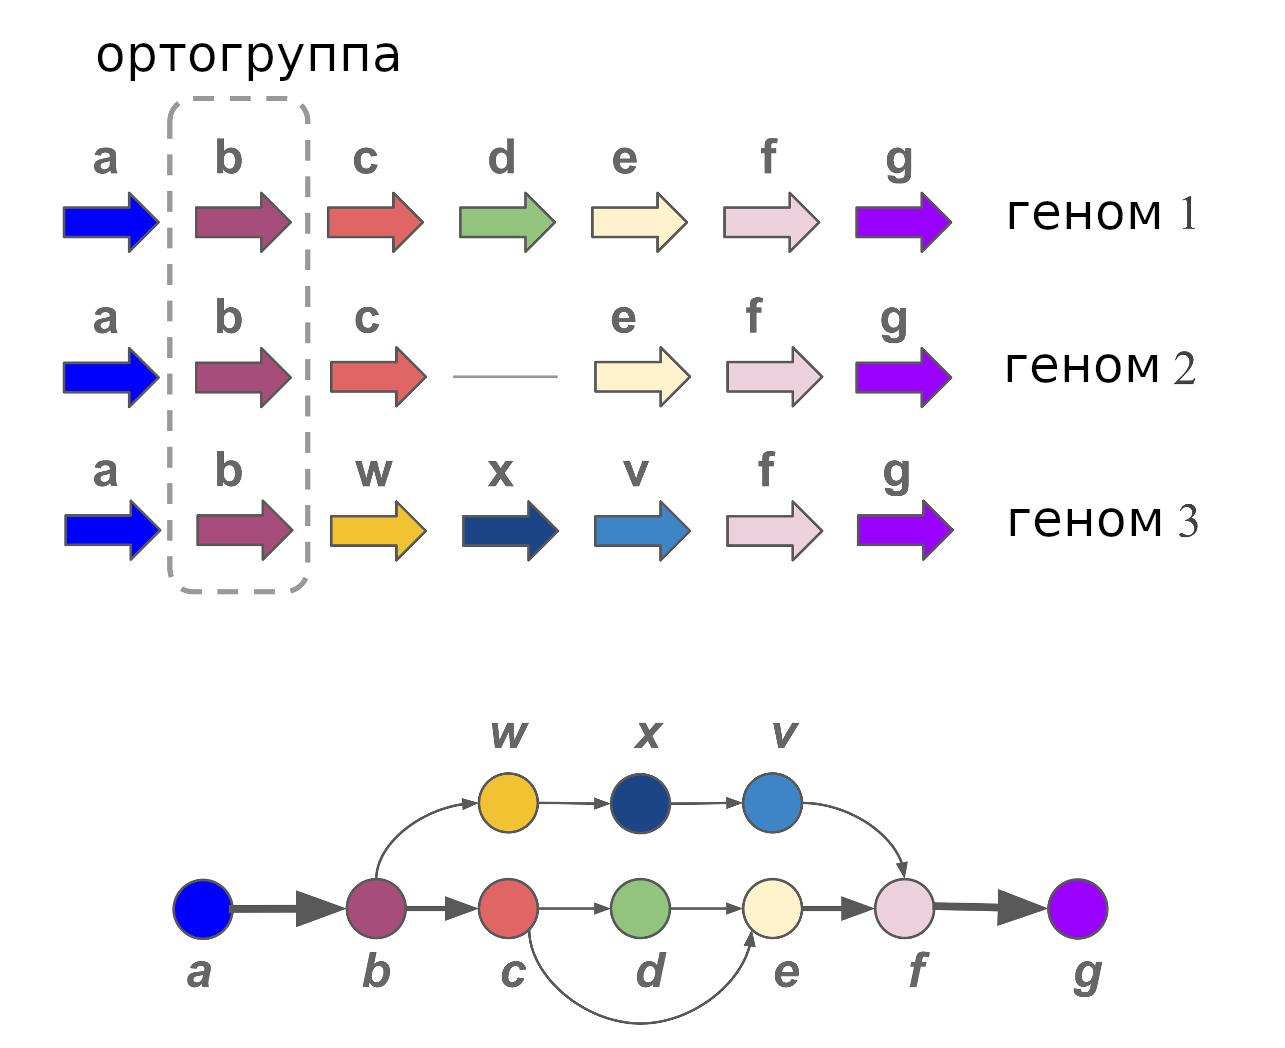
\includegraphics [width=0.9\textwidth] {Dissertation/images/graph/graph_scheme.png}
    \caption{Представление контекста генов в виде графа. Рассматриваем три гипотетеических генома, состоящих из 6-7 генов. Гены показаны стрелками, цветом и буквами обозначены гены, относящиеся к одной ортогруппе. В нижней части рисунка показано графовое представление для данного набора геномов.}
    \label{img:graph_scheme}
\end{figure}

Мы выбрали способ представления  набора геномов в виде направленного графа:  ребра имеют направление, соответствующие обходу генома от начала к концу. Это было сделано для того, чтобы сохранить всю информацию о порядке расположения генов, в частности о геномных инверсиях. Рассматриваемые геномы при этом должны быть ориентированы единообразно. В публичных базах геномов (RefSeq, GenBank, Patric и другие) не предусмотрено требований к ориентации последовательностей: они начинаются с произвольных позиций и могут быть ориентированы в произвольном направлении. Поэтому перед построением графа, мы производим согласование ориентаций геномов друг с другом. Для этого выбирается референсный геном (произвольно, из финишированных геномов), затем для каждого генома устанавливаются области синтении (относительно референсного генома); подсчитывается сумма произведений длин блоков на нуклеотидное сходство для всех блоков в прямой и обратной ориентации; в зависимости от того, какая из сумм оказалась выше, оставляется либо исходная ориентация, либо она меняется на противоположную. Если рассматриваемый геном состоит из нескольких контигов, то согласование ориентации с референсом производится для каждого контига в отдельности.

Скрипт на языке R, выполняющий согласование ориентаций генома и построение графа доступен по адресу \url{https://github.com/paraslonic/graph_complexity/scripts/OG2graph.r}. На вход ему подается таблица групп гомологии в формате выдачи программы OrthoFinder - текстовый файл, каждая строка которого соответствует одной группе гомологии и имеет формат: <идентификатор группы>: <ген1> <ген2> ... <ген n>. На выходе создается файл paths.sif, содержащий граф в формате sif: <идентификатор группы 1> <идентификатор группы 2> <геном>. 

Для автоматизации представления набора геномов в виде графа мы реализовали вычислительный конвейер, схема которого представлена на рисунке~\ref{img:graph_pipe_schema}. В нем осуществляются следующие шаги: 1) аннотация геномов (выделение белок-кодирующих областей), 2) форматирование файла в формате FASTA с аминокислотными последовательностями генов (в заголовках последовательностей мы указываем информацию о расположении генов), 3) построение групп гомологий и 4) формирование графа. На вход подается набор нуклеотидных последовательностей геномов в формате FASTA, выходом является граф в формате sif. Данный конвейер реализован в системе управления рабочим процессом snakemake и доступен по адресу \url{https://github.com/paraslonic/graph_complexity}.

\begin{figure}[!ht] 
  \center
    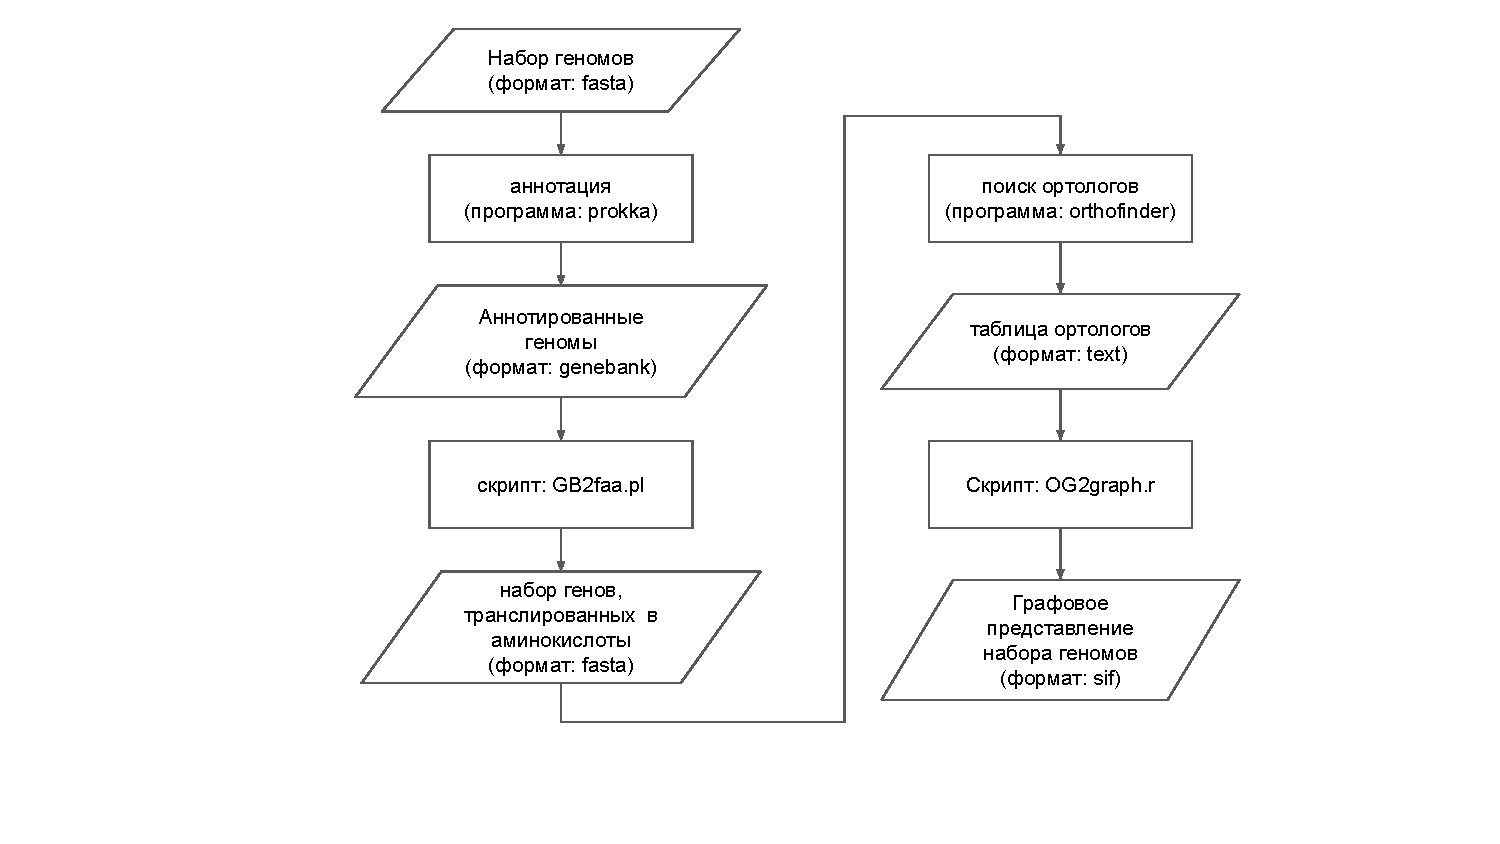
\includegraphics [width=\textwidth] {Dissertation/images/graph/graph_complexity_schema.pdf}
    \caption{Вычислительный конвейер для представления контекста генов в наборе геномов в виде графа.}
    \label{img:graph_pipe_schema}
\end{figure}

\subsection{Разработка алгоритма оценки изменчивости генома на основе графового представления}

Предположим, что в ходе эволюции, в рассматриваемой группе геномов, наблюдались лишь изменения микро-масштаба -- однонуклеотидные замены. В таком случае, набор и взаимное расположение генов не изменялись и соответствующий граф будет содержать лишь один путь. Любые изменения в составе, либо расположении, генов (делеции, вставки, перемещения) будут приводить к появлению новых ребер и новых узлов (в случае вставки нового гена). Чем больше узлов и ребер содержит граф --- тем больше возможных путей его обхода. Это позволяет использовать количество путей в графе в качестве меры вариабельности генома.

Разные фрагменты генома могут существенно различаться по уровню изменчивости. Ниже мы опишем процедуру построения профиля изменчивости генома. Данный профиль отражает как уровень изменчивости меняется вдоль хромосомы (либо иного репликона). Для подсчета уровня локальной изменчивости в отдельном фрагменте генома происходит подсчет количества путей в подмножестве графа (подграфе), соответствующему данному фрагменту. Локальная изменчивость подсчитывается во всех возможных локусах генома и таким образом получается профиль изменчивости. Иначе говоря, мы проходим по геному скользящим окном, выбирая области фиксированного размера (ширина окна задается пользователем) и оцениваем количество зафиксированных изменений в этих областях.

Принцип подсчета локальной вариабельности генома проиллюстрирован на рисунке~\ref{img:complexity_scheme}. Из множества геномов выбирается один геном, служащий референсом (для него будет производиться построение профиля вариабельности). Путь, соответствующий чередованию генов в референсном геноме будем называть базовым путем (узлы этого пути обозначены зеленым цветом). Рассмотрим некоторую окрестность гена Х, ограниченную тремя генами слева и справа от гена Х. Произведем поиск путей, которые начинаются (исходят из базового пути) и заканчиваются (возвращаются в базовый путь) внутри рассматриваемой окрестности и при этом не проходят через узел Х --- такие пути будем называть обходными путями. Суммарное количество обходных путей принимается в качестве меры локальной вариабельности генома окрестности гена Х. На нижней части рисунка~\ref{img:complexity_scheme} показаны примеры: слева --- участка с низкой вариабельностью и двумя обходными путями, справа --- с более высокой вариабельностью и шестью обходными путями. Для получения профиля вариабельности, мы рассчитываем локальную вариабельность для каждого гена из референсного генома.  

\begin{figure}[!ht] 
  \center
    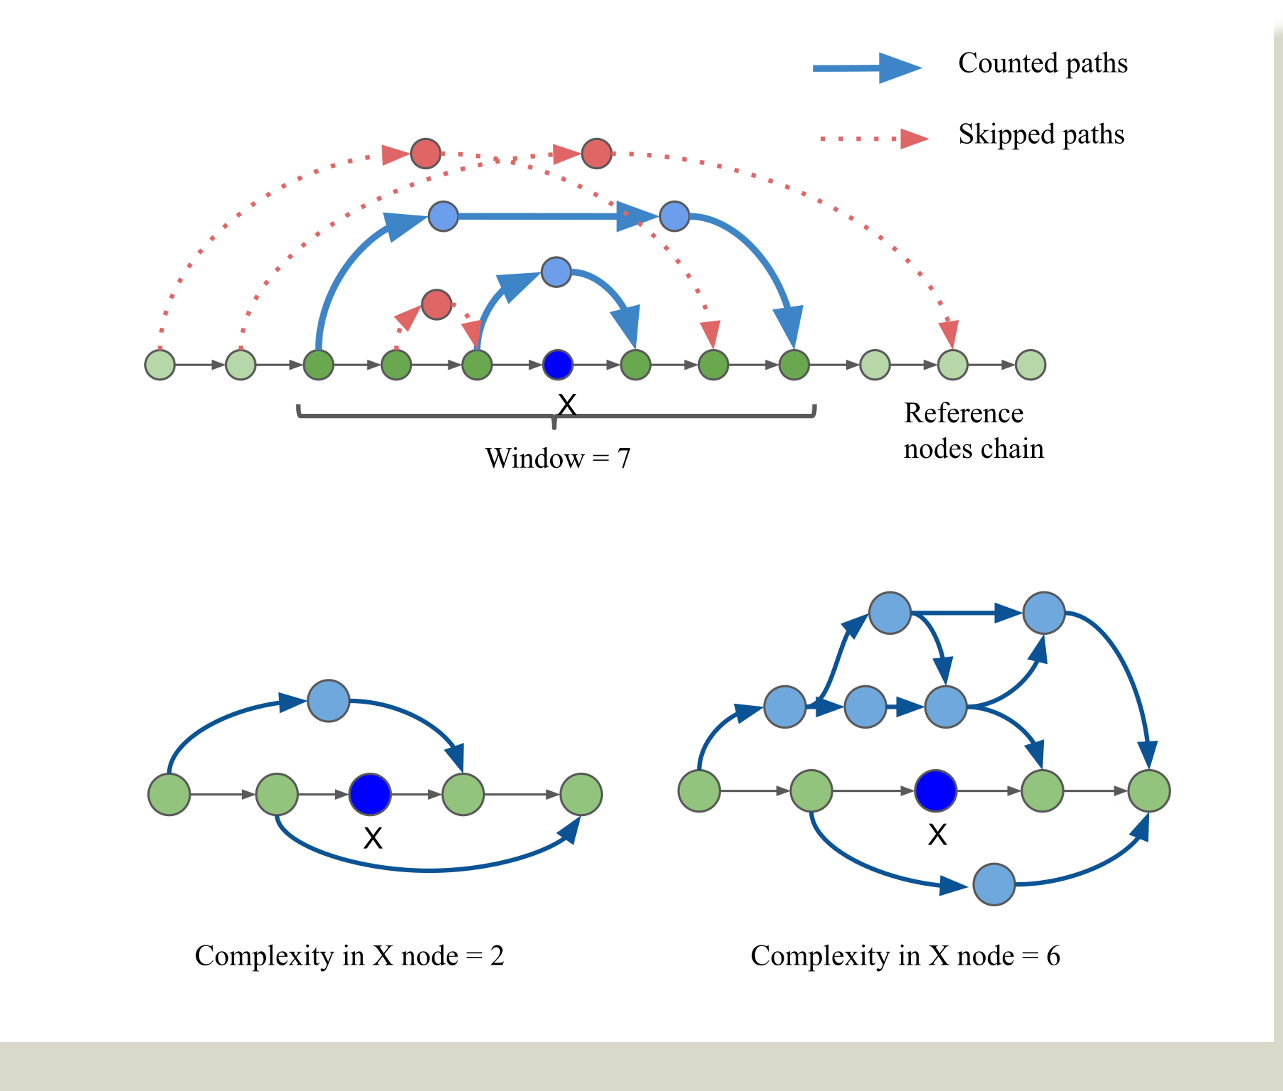
\includegraphics[width=0.8\textwidth]{Dissertation/images/complexity_scheme.png}
  \caption{Подсчет локальной вариабельности генома на основе количества путей в графе. Вверху показан подграф, представляющий окрестность гена X. Ребра черного цвета являются частью базового пути, который соответствует порядку генов в референсном геноме, ребра синего цвета --- обходным путям, а ребра красного цвета --- путям, которые не вносят вклад в значение вариабельности. На нижней части рисунка приведен пример графа с низкой (слева) и высокой (справа) вариабельностью, указаны соответствующие количества обходных путей.}
  \label{img:complexity_scheme} 
\end{figure}



%###########################################################################################

\subsection{Верификация предложенного метода оценки профиля изменчивости генома}
Мы провели верификацию предложенного подхода оценки профиля изменчивости и его программной реализации при помощи: 1) симуляции эволюции геномов; 2) сравнения результатов нашего метода с ранее опубликованными оценками других авторов. 

\subsubsection{Симуляция эволюции геномов}
Мы проводили моделирование эволюции геномов на основе задаваемого профиля изменчивости. Данный профиль определял вероятности изменений генного состава в зависимости от положения гена в геноме. Мы использовали следующие варианты изменений: вставки либо удаления генов, перемещения генов, инверсии фрагментов моделируемого генома. Мы использовали несколько профилей изменчивости, для каждого из которых проводили моделирование геномных изменений, оценивали профиль изменчивости предложенным нами методом и сравнивали полученный результат с изначально заданным профилем. Нашей целью была проверка применимости предложенного метода в том случае, когда в геноме присутствуют области пониженной и повышенной изменчивости.

Модельный геном представлял из себя последовательность целых чисел (n=5000). Вначале, создавались одинаковые геномы. Далее, проводилось 3000 итераций, в каждой из которых происходило изменение генома. Локализация изменений определялась на основе профиля изменчивости. Вероятности вставки и удаления генов были выбраны равными друг другу (для сохранения длины геномов), вероятности геномных инверсий были в 100 раз меньше (оценка получена исходя из литературных данных). Длины инверсий, вставок и делеций выбиралась случайно, на основе экспоненциального распределения (изменения малой длины были более вероятны, чем изменения большой длины). Вставка генов производилась из набора, размер которого в два раза превышал исходный набор генов (исходно в геноме были числа от 0 до 5000, вставлялись числа от 5000 до 15000).

Профили изменчивости были следующих типов: 1) ступенчатый, 2) синусоидальный, 3) пилообразный. Для каждого профиля изменчивости проводилось 10 симуляций. На рисунке~\ref{img:simulation} приведен пример сравнений исходного профиля изменчивости (слева) и профиля, полученного в результате анализа предложенным нами способом (справа). В таблице \ref{simulation_table} приведены средние значения R$^{2}$ и коэффициента корреляции исходного профиля изменчивости и профиля, полученного в результате анализа и усредненного по 10 повторам. 

\begin{figure}[!ht] 
  \center
    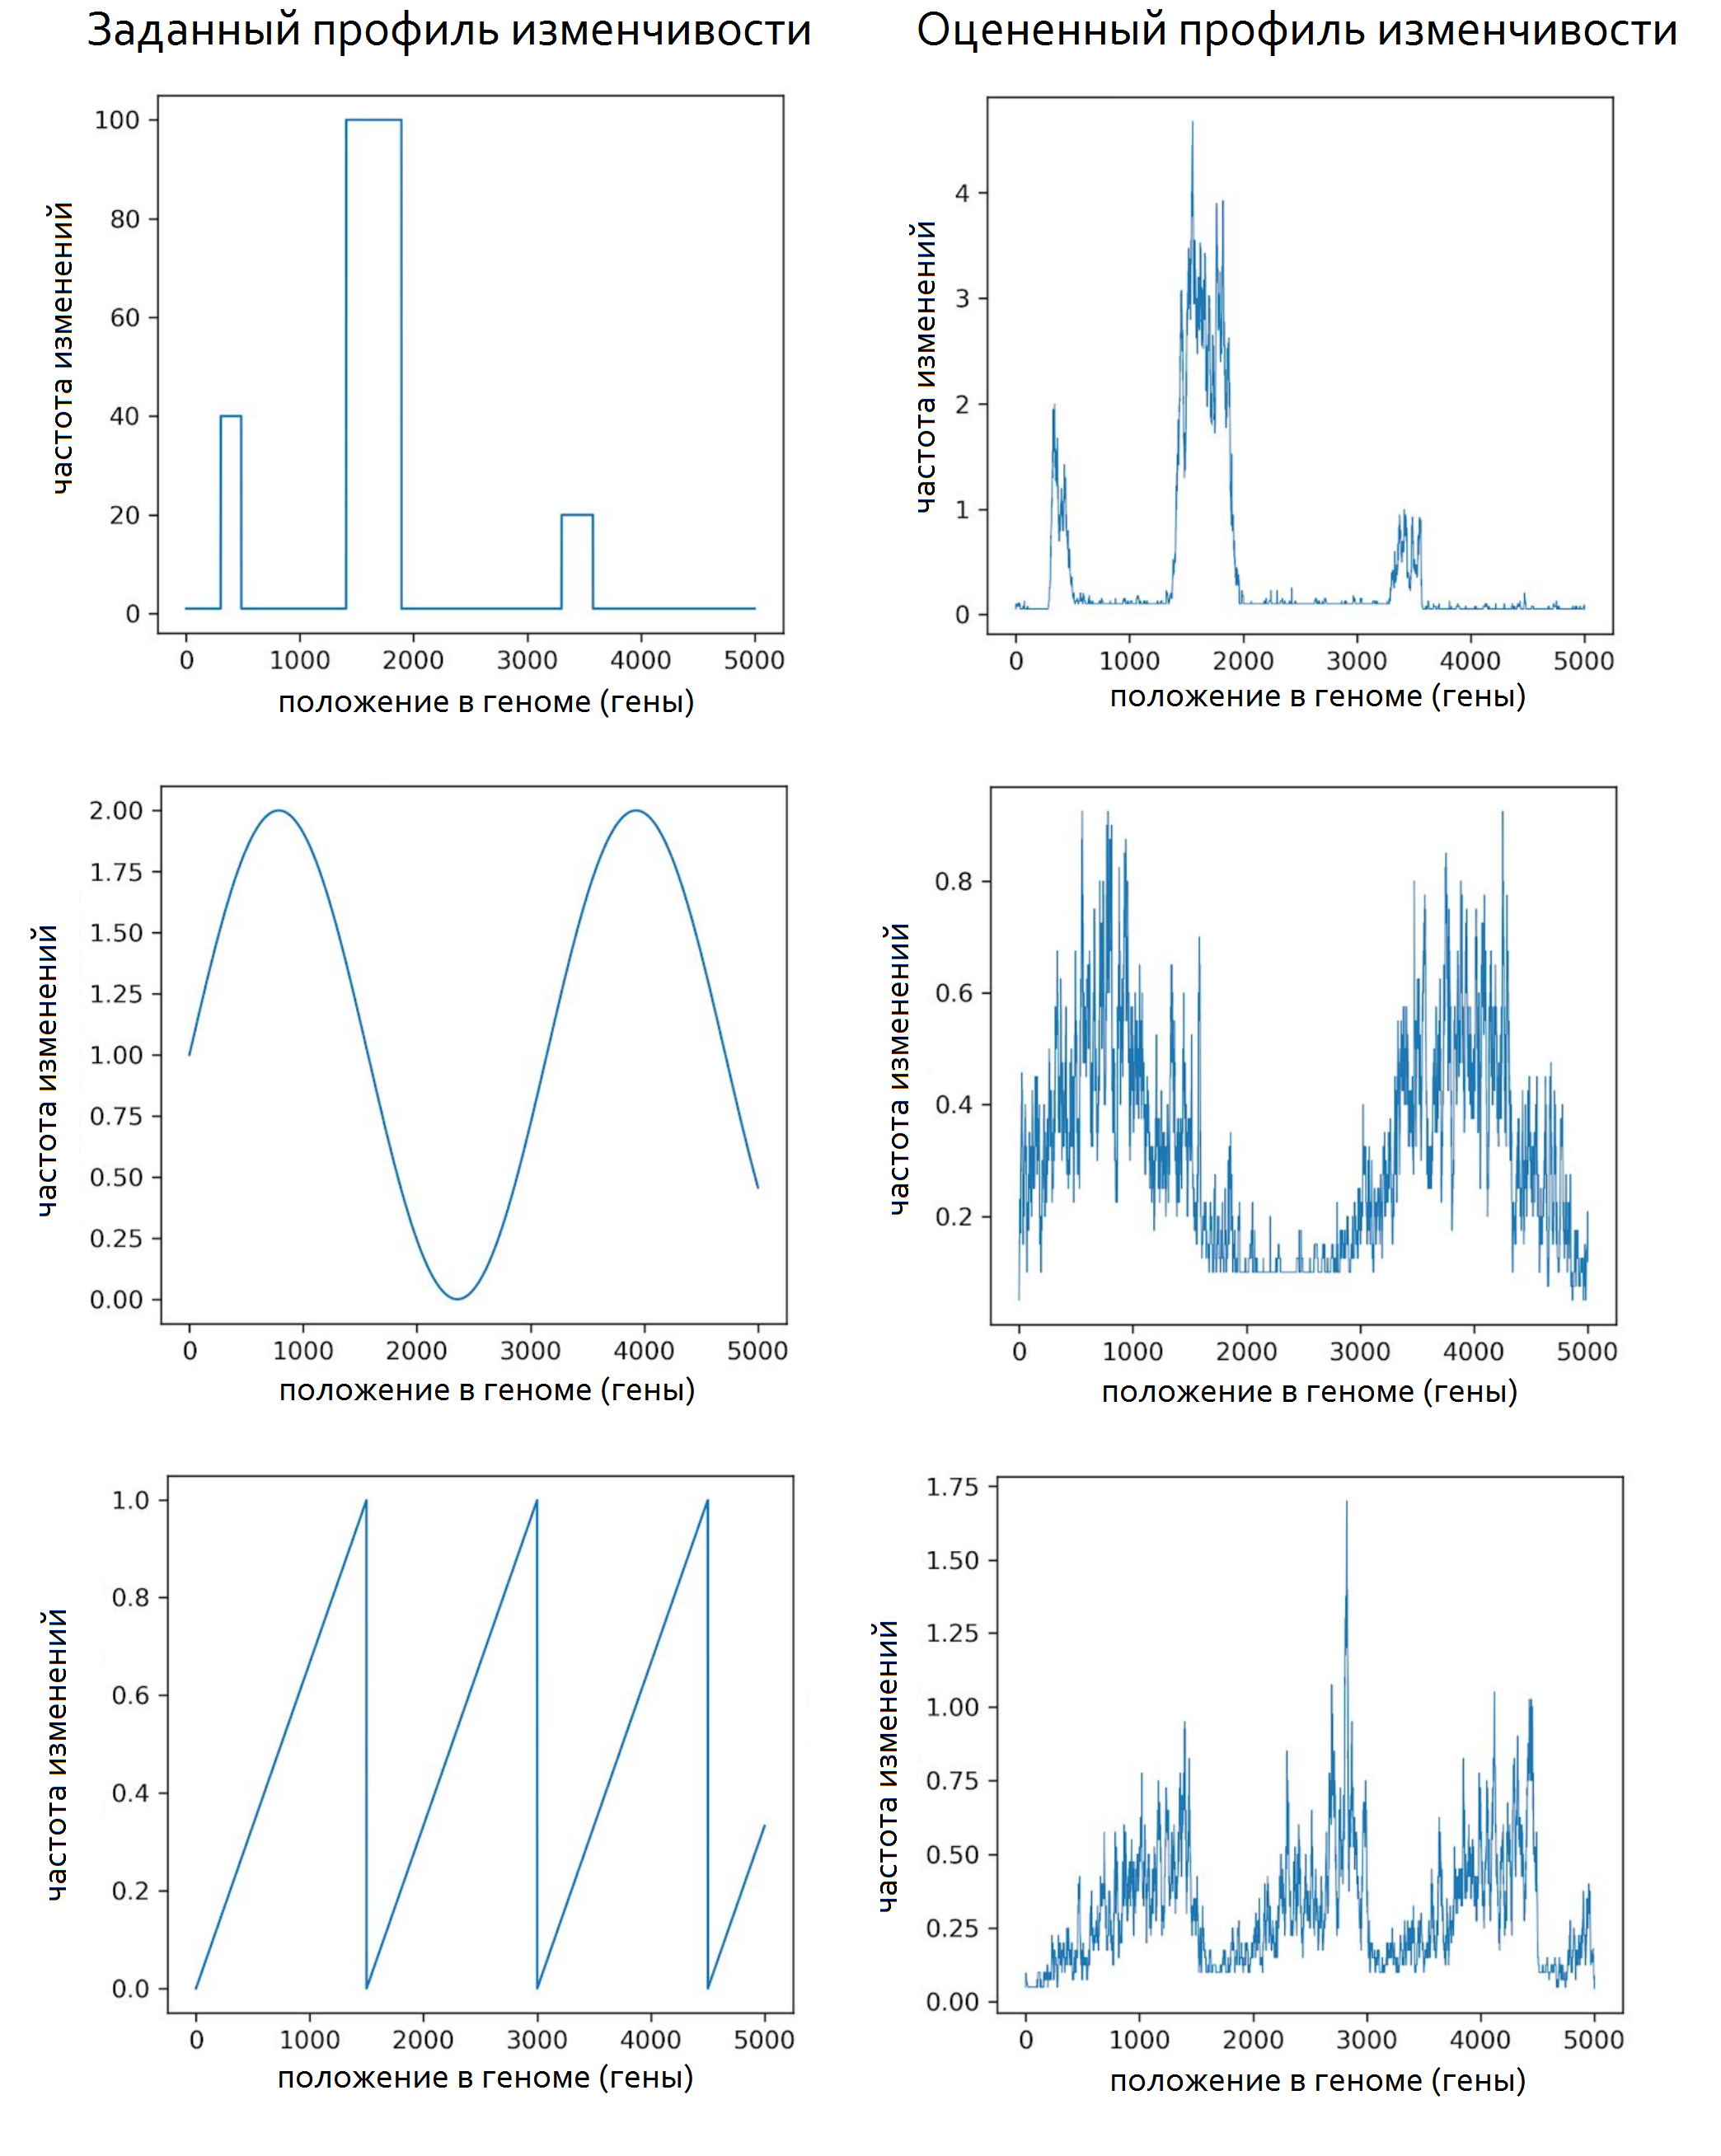
\includegraphics[width=0.8\textwidth]{Dissertation/images/complexity/simulation.png}
  \caption{Сравнение профиля изменчивости, задаваемого для моделирования геномных изменений (слева), и профиля, получаемого в результате анализа предложенным нами методом (справа). }
  \label{img:simulation} 
\end{figure}

\begin{table} [htbp]
  \centering
  \parbox{15cm}{%
      \caption{Результаты сравнения задаваемого при моделировании и оцененного профиля изменчивости при разной форме профиля.}\label{simulation_table}%
  }
\begin{tabular}{ | l | l | l | }
\hline
Тип профиля & Значение R$^{2}$ & Коэффициент корреляции Спирмена\\ \hline
Ступенчатый & 0.95 & 0.69 \\ \hline
Синусоидальный & 0.77 & 0.82 \\ \hline
Пилообразный & 0.80 & 0.85 \\ 
\hline
\end{tabular}
\end{table}

Отметим, что значительное влияние на точность оценки профиля изменчивости оказывает частота геномных инверсий: чем она выше - тем была ниже точность. Таким образом, частые перестройки генома служат существенным ограничением применимости предложенного метода. 

\subsubsection{Сравнения результатов предложенного метода с ранее опубликованными оценками других авторов}
В работе \cite{oliveira2017chromosomal} авторы проводили поиск горячих точек горизонтального переноса генов (ГПГ) для 80 бактериальных видов. Мы провели сравнение найденных ими горячих точек с профилем изменчивости генома, оцененным описанным выше способом. На рисунке~\ref{img:rocha_comparison} приведен пример сравнения результатов двух методов для генома \textit{E. coli}. Видно, что, в данном случае, оба метода хорошо согласуются между собой.     

\begin{figure}[!ht] 
  \center
    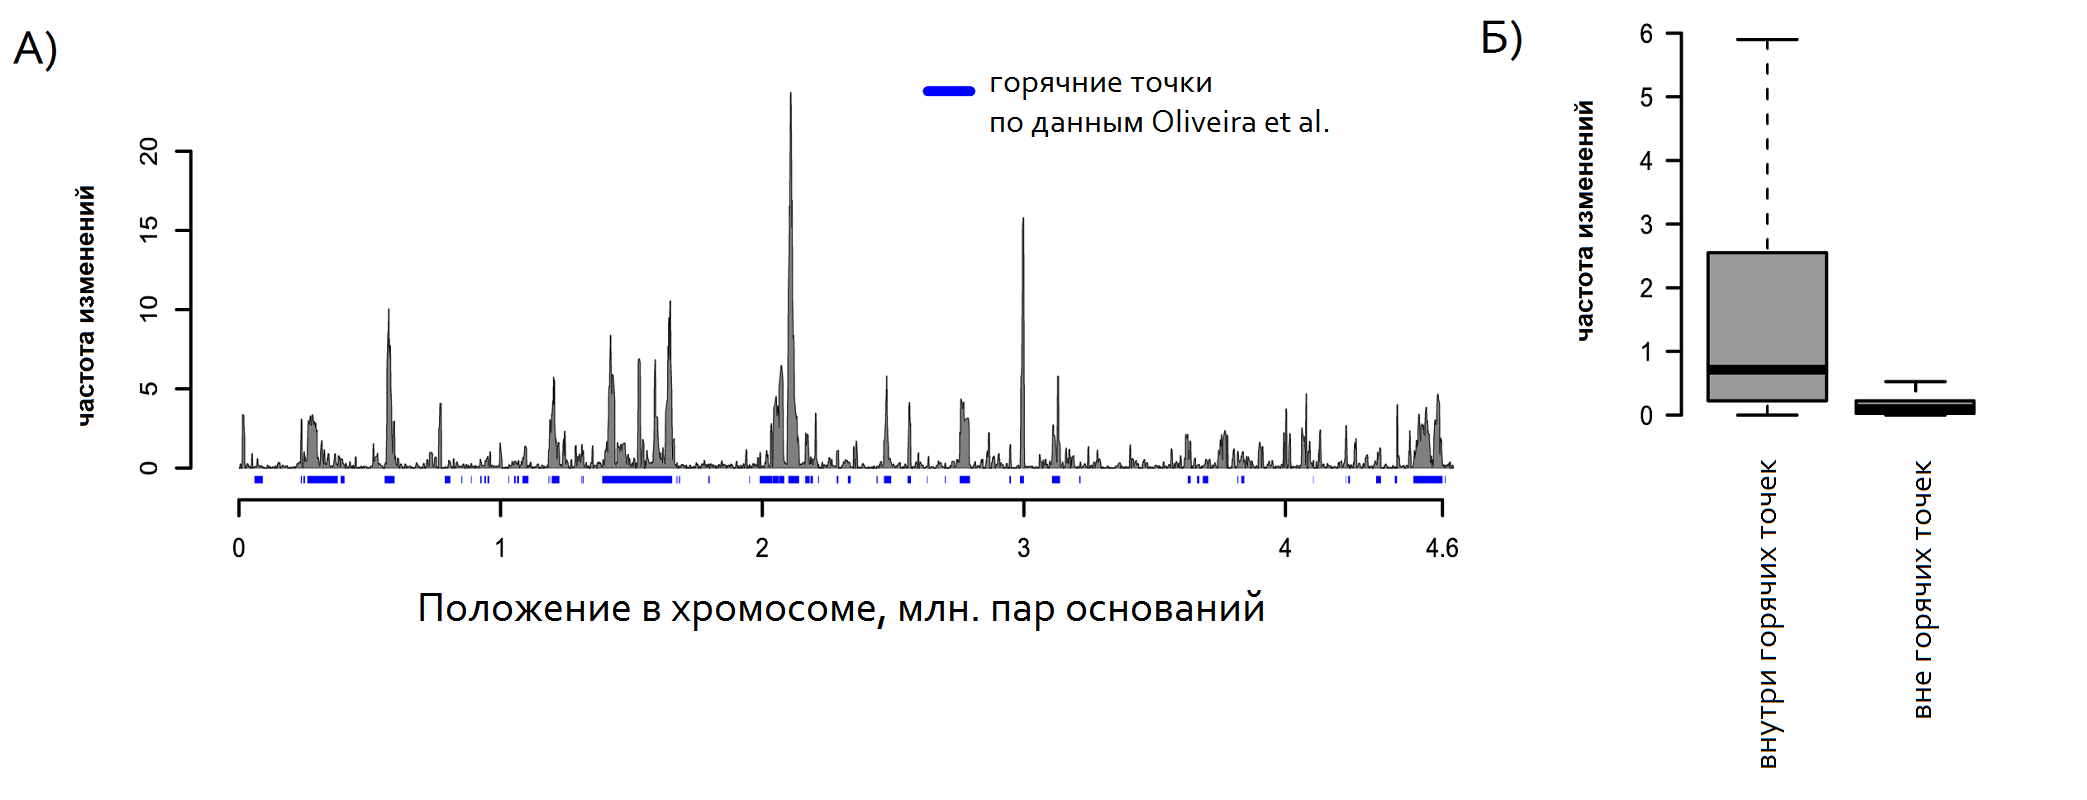
\includegraphics[width=\textwidth]{Dissertation/images/complexity/rocha_comparepng.png}
  \caption{Сравнение профиля изменчивости \textit{E. coli K12 MG1655}, установленного нашим методом, с областями повышенной изменчивости (``горячими'' точками горизонтального переноса) генов в работе Oliveira et al. \cite{oliveira2017chromosomal}. }
  \label{img:rocha_comparison} 
\end{figure}

Для других видов бактерий, мы наблюдали как хорошо согласующиеся между собой, так и весьма непохожие результаты (например, в случае \textit{Brucella melitensis} и \textit{Burkholderia pseudomallei}). Расхождение может быть следствием: 1) малого количества геномов используемого для анализа в работе \cite{oliveira2017chromosomal} (для многих видов оно было меньше 20, в среднем 12 геномов для одного вида), что значительно ухудшает соотношение сигнал/шум как нашего, так вероятно и используемого в работе \cite{oliveira2017chromosomal} метода, 2) различием в подходах для оценки изменчивости (мы берем в рассмотрения все события, затрагивающие изменение порядка генов, не только горизонтальный перенос генов). Выяснение точной причины расхождений затруднено, поскольку авторами работы \cite{oliveira2017chromosomal} не предоставляется программная реализация метода.

%###########################################################################################
\section{Исследование применимости метода оценки локальной вариабельности генома}

\subsection{Зависимость результатов от размера выборки}

Чем больше геномов будет использовано для анализа, тем полнее будет получено представление о возможных вариантах со-расположения генов. Слишком маленькое количество геномов приведет к понижению чувствительности анализа и снизит соотношение сигнал/шум. В тоже время, слишком большое количество геномов потребует значительных вычислительных ресурсов и приведет к увеличению времени анализа. Поэтому, актуален вопрос о зависимости результатов анализа от размера выборки и определение минимально допустимого количества геномов.

На рисунке~\ref{img:genome_number} показан график зависимости коэффициента корреляции профиля вариабельности, рассчитанного на основании 100 геномов, либо на основании выборки меньшего размера. Для анализа использованы финишированные геномы \textit{E. coli}. Для каждого размера выборки геномов проводилось 10 испытаний, для чего геномы выбирались случайным образом из полного набора. 

\begin{figure}[!ht] 
  \center
    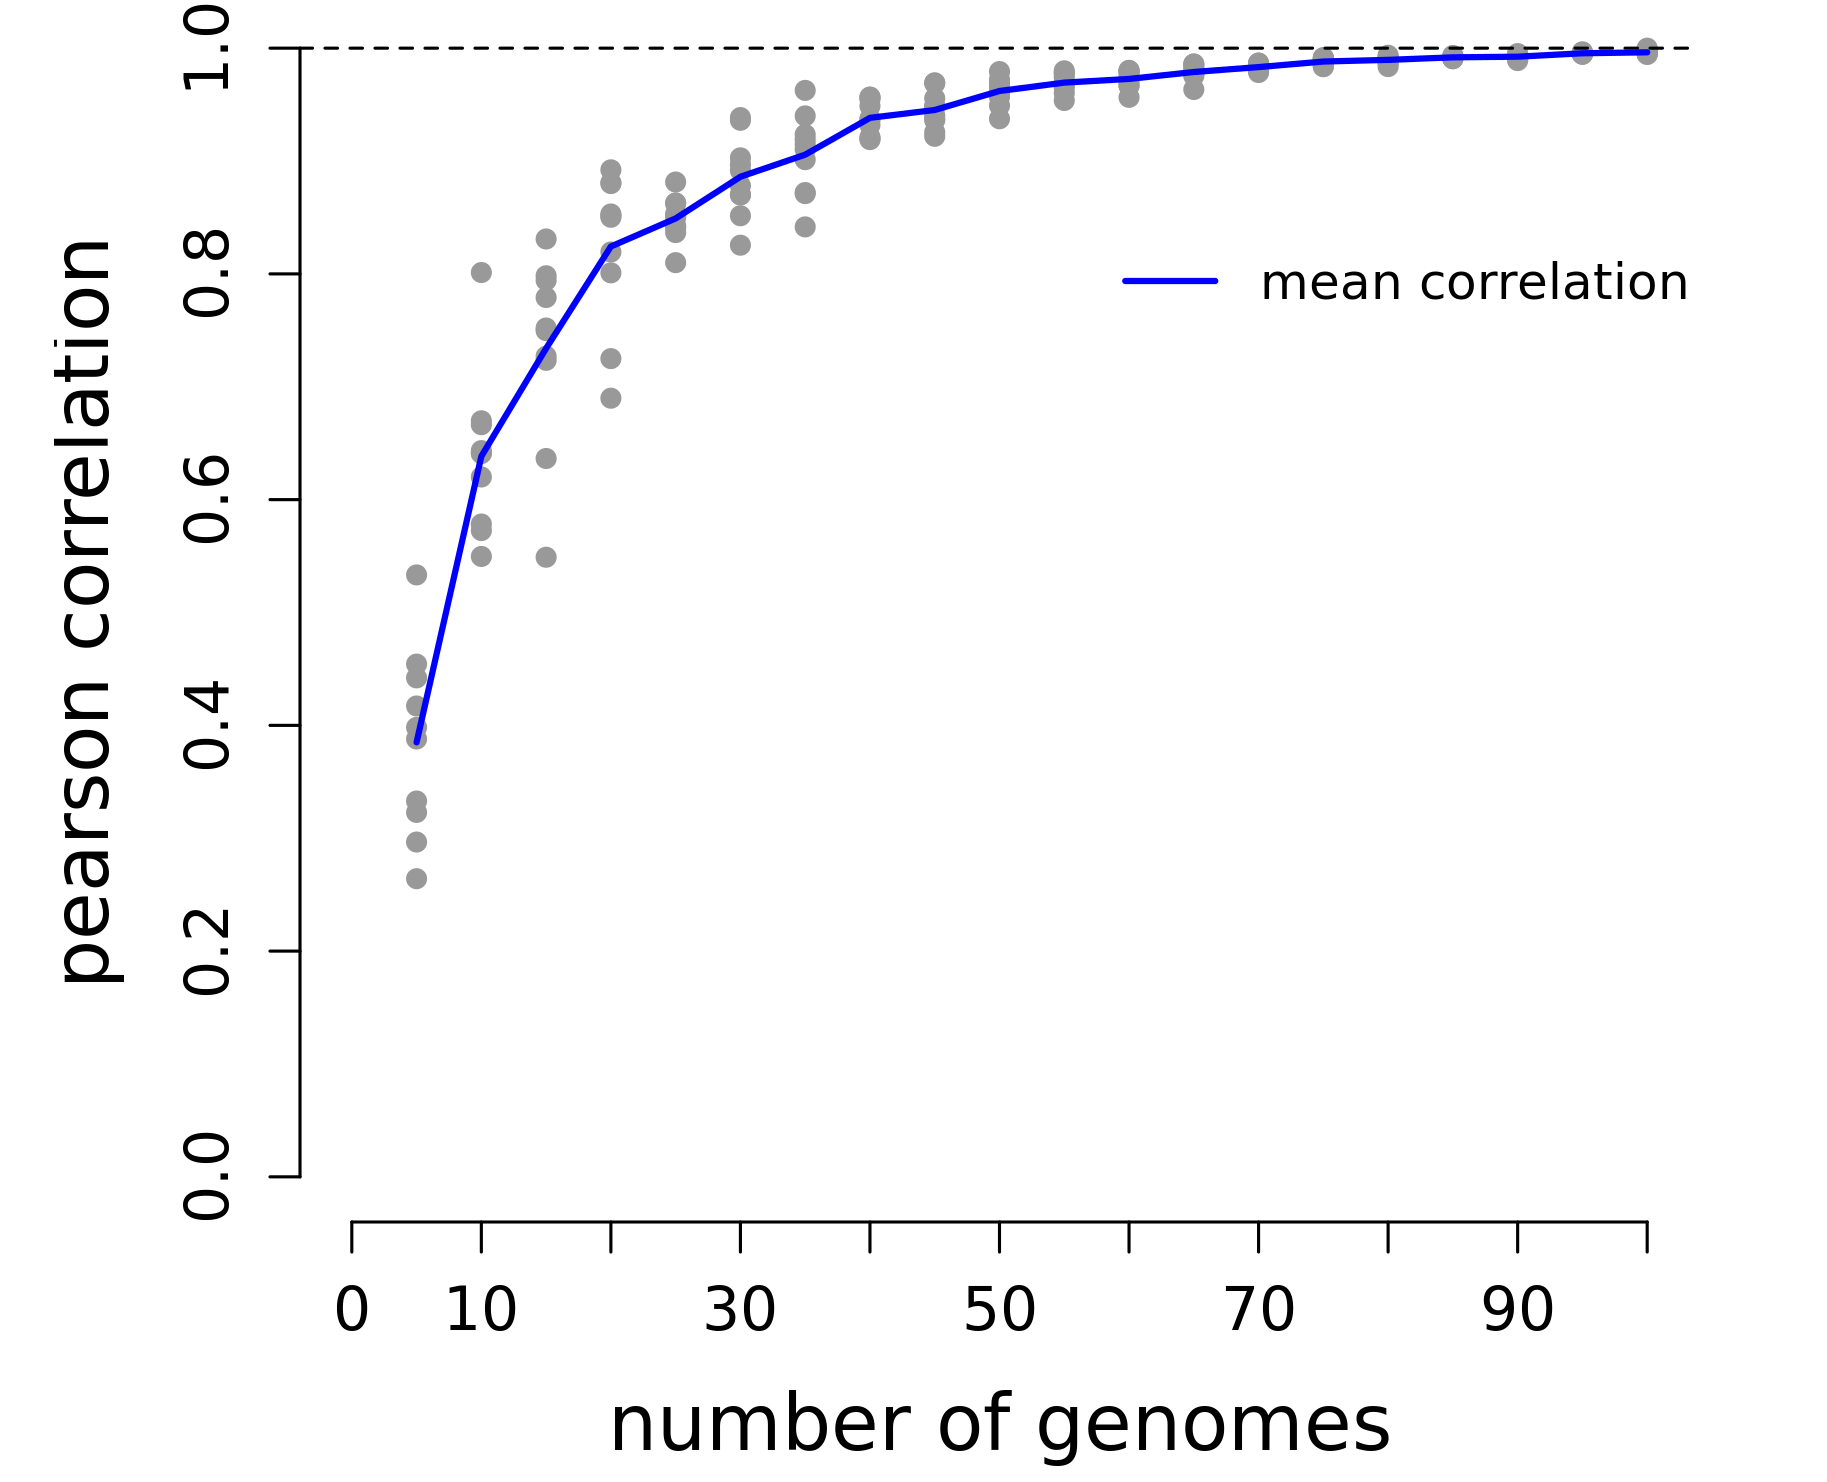
\includegraphics[width=0.5\textwidth]{Dissertation/images/complexity/numberOfGenomes.png}
  \caption{Значение коэффициента корреляции профиля вариабельности, оцененной на основе 100 геномов с профилями оцененными на основе меньшего количества геномов. Синяя линия проведена по значениям корреляции, усредненным по 10 испытаниям. }
  \label{img:genome_number} 
\end{figure}

При количестве геномов большем чем 50, значение коэффициента корреляции превышало уровень 0.9. В дальнейшем, мы ориентировались на эту оценку и брали в рассмотрение лишь те виды, для которых доступное количество геномов составляло не менее 50.

На рисунке~\ref{img:complex_runtime} показана зависимость времени, необходимого для построения графа и анализа профиля вариабельности от количества геномов. Анализ проводился на основании финишированных геномов \textit{E. coli}. Видно, что зависимость носит линейный характер. Анализ проводился в один поток на персональном компьютере с процессором i7 9750h. Наиболее продолжительным шагом общего анализа является этап построения групп гомологии. Так, для тысячи геномов, время анализа составило пять суток, анализ проводился в 50 потоков на вычислительном кластере на основе процессоров AMD EPYC 7502.

\begin{figure}[!ht] 
  \center
    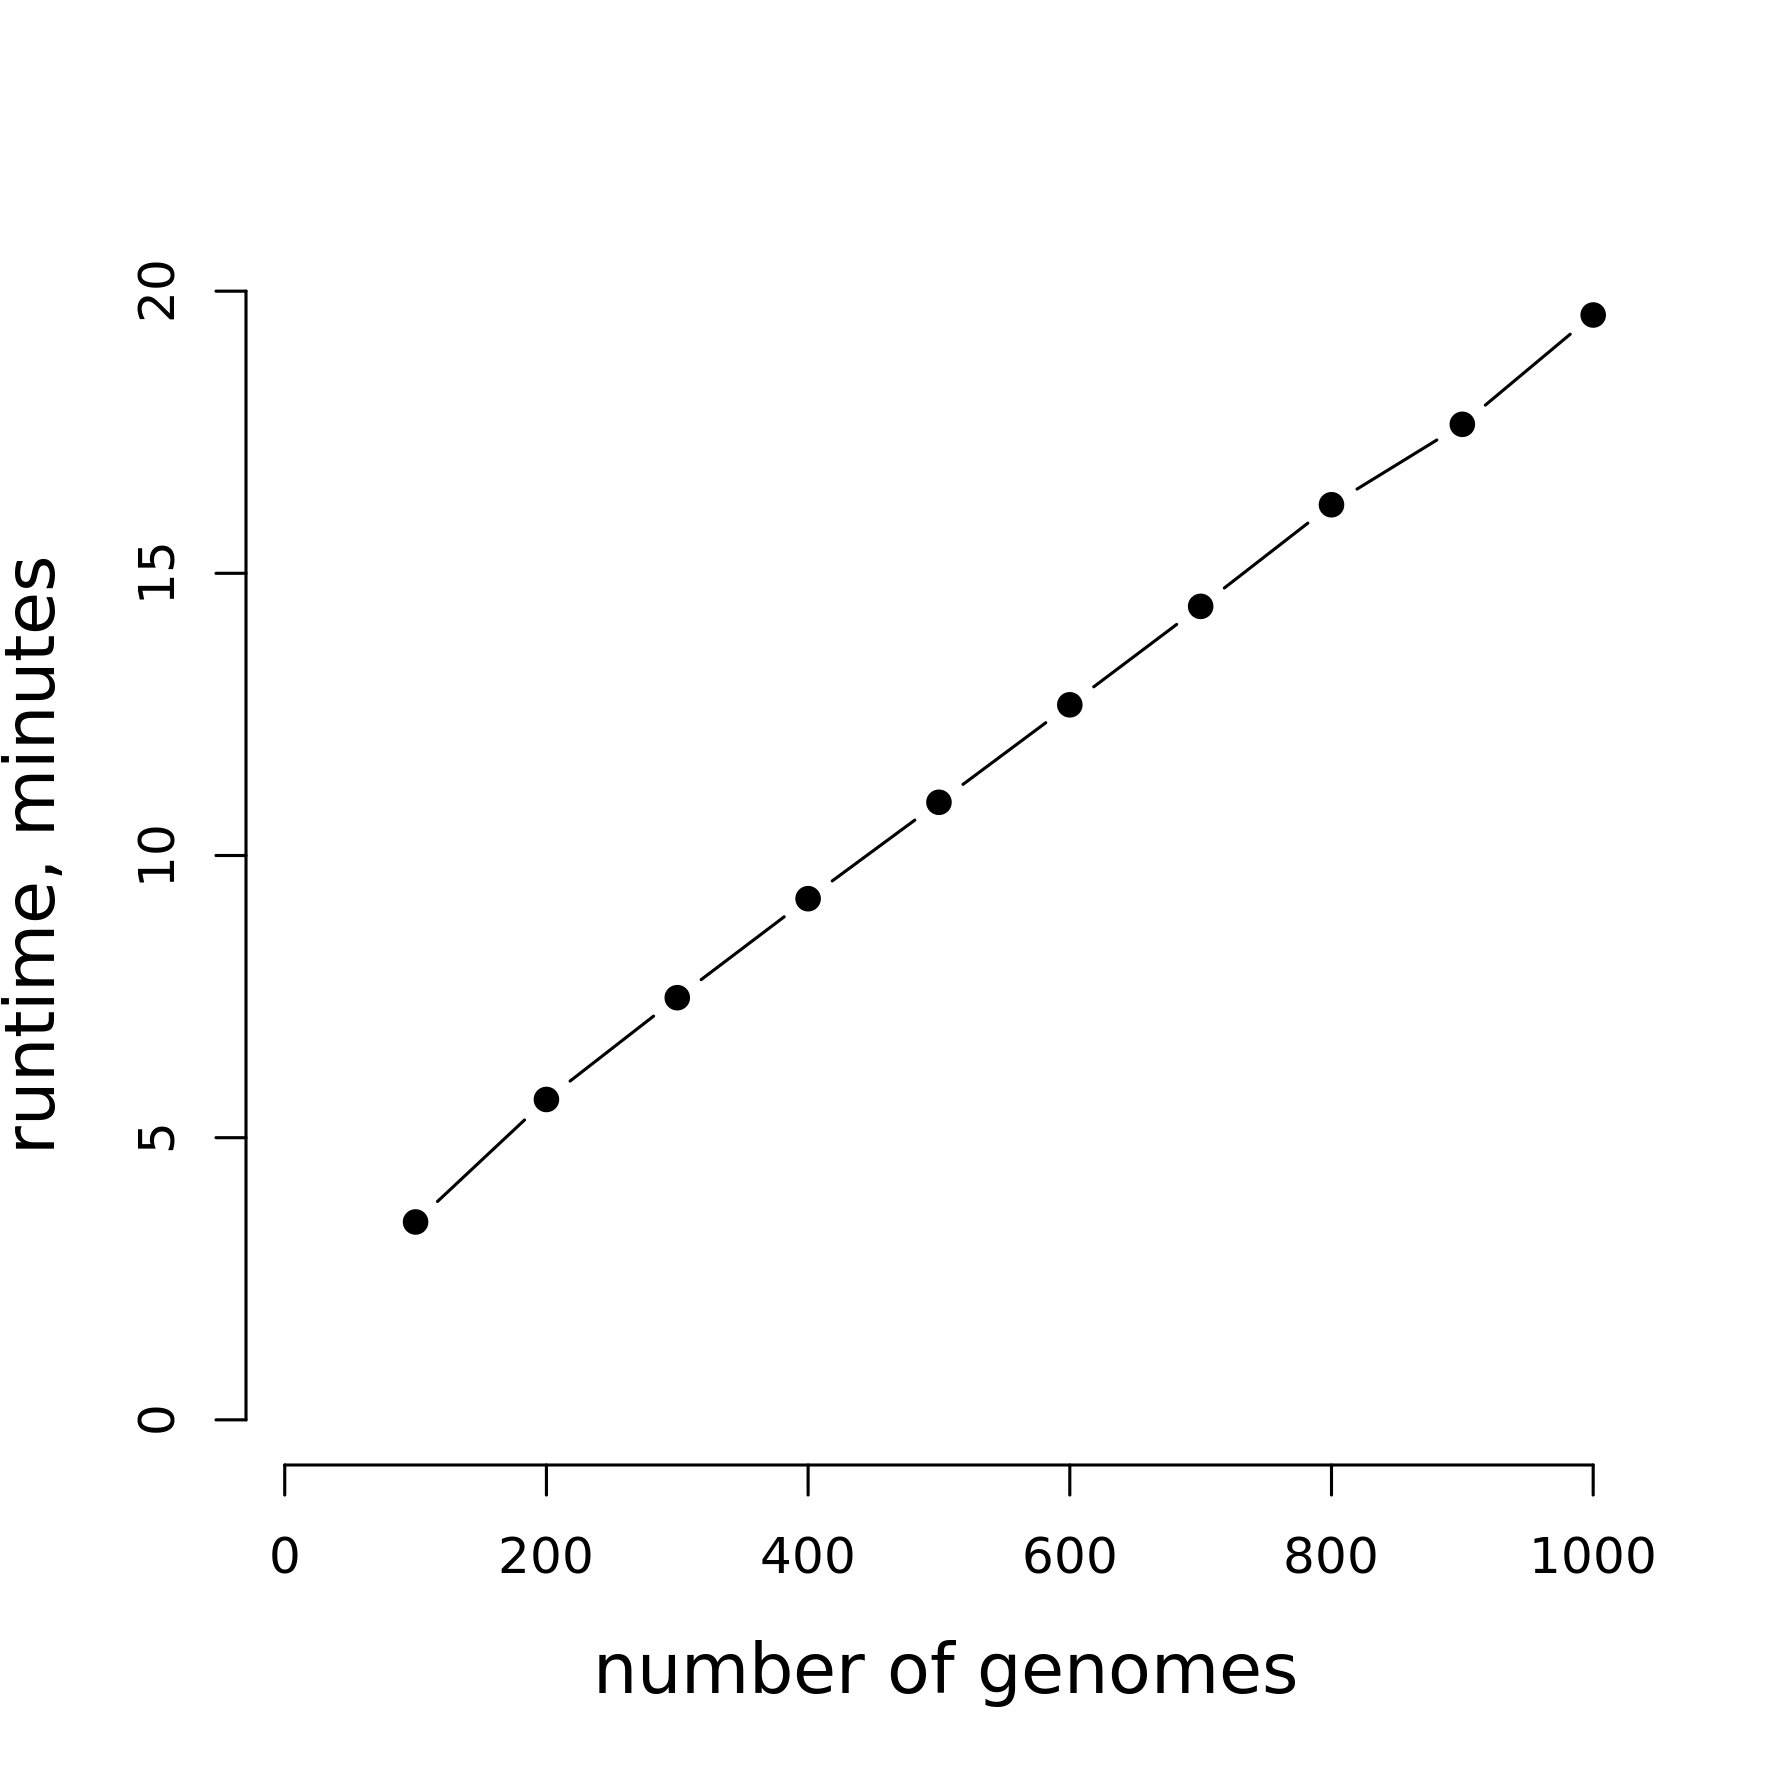
\includegraphics[width=0.8\textwidth]{Dissertation/images/complexity/runtime_nocoalign.png}
  \caption{Зависимость времени, необходимого для построения графа и расчета профиля изменчивости, от количества геномов. Для анализа использованы финишированные геномы \textit{E. coli}. }
  \label{img:complex_runtime} 
\end{figure}

\subsection{Анализ зависимости результатов от качества сборки генома}

Многие геномы прокариот собраны не до уровня репликонов, но состоят из контигов - фрагментов генома, которые удается собрать из коротких прочтений, без применения дополнительных экспериментальных методов. 
Для анализа чувствительности алгоритма к типу входных данных: финишированные (собранные до уровня репликонов), либо фрагментированные геномы (состоят из контигов), мы выбирали случайным образом по 100 геномов одного либо другого типа и оценивали профили вариабельности по одному и тому же референсному геному. Сравнение профилей по финишированным либо фрагментированным геномам для двух видов бактерий показано на рисунке~\ref{img:compl_dr_coli}. Видно, что профили обладают значительной степенью сходства (коэффициент корреляции Пирсона составил 0.87 и 0.81 для \textit{E. coli} и \textit{Pseudomonas aeruginosa}, соответственно). 

\begin{figure}[!ht] 
  \center
    \subcaptionbox{}{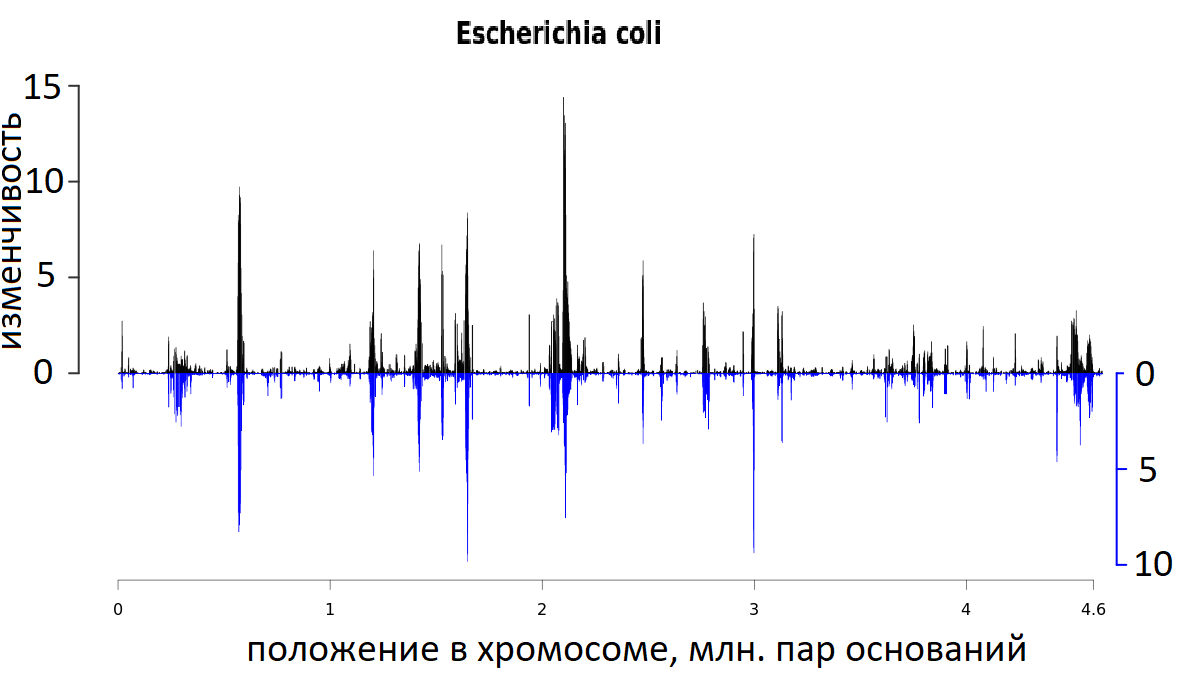
\includegraphics[width=0.8\textwidth]{Dissertation/images/complexity/complete_draft_coli.png}}
    \subcaptionbox{}{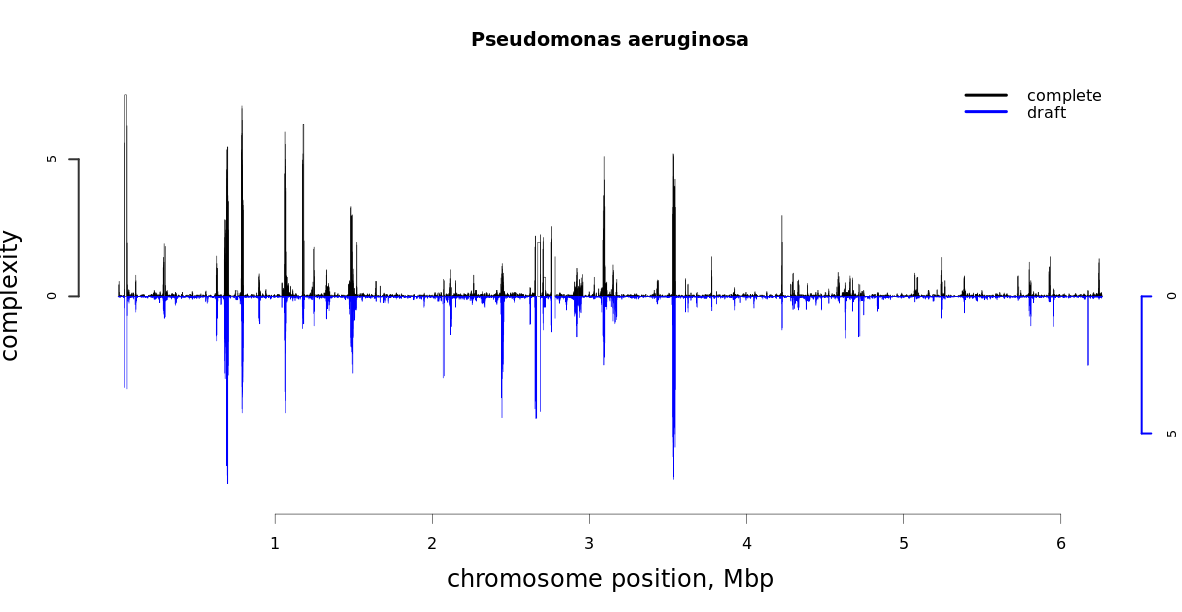
\includegraphics[width=0.8\textwidth]{Dissertation/images/complexity/complete_draft_paeru.png}}
  \caption{Сравнение профилей вариабельности 100 финишированных и 100 фрагментарных геномов видов: а) \textit{E. coli}, б) \textit{Pseudomonas aeruginosa}. Черным цветом показан профиль вариабельности на основе финишированных геномов, синим - на основе собранных до уровня контигов.}
  \label{img:compl_dr_coli} 
\end{figure}

Заметим, что значения профиля изменчивости зависят от набора геномов, используемых для сравнения. Мы выбирали случайные геномы в наборы финишированных и фрагментированных геномов, что также вносило вклад в наблюдаемое различия профилей. Вклад собственно качества сборки геномов еще меньше наблюдаемого выше уровня различий. Основываясь на этой оценке, мы считали, что финишированность геномов не является обязательным для включения геномов в анализ.

%№№№№№№№№№№№№№№№№№№№№№№№№№№№№№№№№№№№№№№№№№№№№№№№№№№№№№№№№№№№№№№№№№№№
\section{Применение метода оценки локальной вариабельности генома}


\subsection{Профиль вариабельности генома \textit{E. coli}}
На рисунке~\ref{img:complexity_lf82} показан профиль изменчивости генома \textit{E. coli LF82}, рассчитанный на основании графового представления 326 геномов других штаммов данного вида. Цветом обозначены жизненно-необходимые гены (мутации в которых летальны), гены транспортных и рибосомных РНК, острова патогенности и места встройки профагов, описанные для данного генома. Видно, что большая часть локусов с повышенной вариабельностью ("горячие точки"\ изменчивости) находятся именно в тех местах, где у данного штамма находятся профаги, либо острова патогенности. Гены транспортных и рибосомных РНК не имеют очевидной связи с профилем вариабельности. 

Отметим, что фрагмент генома с наибольшим уровнем вариабельности (расположен в области 2,115,791-2,164,382 п.о.) не содержит описанных детерминант мобильности ДНК ни в референсном геноме, ни в геномах других штаммов используемых для анализа. Наиболее консервативный набор генов в этом региона следующий: имидазол-глицерин фосфат синтаза, 1-(5-фосфорибозил)-5-[(5-фосфорибозиламино) метилиденамино] имидазол-4-карбоксамид изомераза, имидазол-глицерин фосфатсинтаза, фосфорибозил-АМФ циклогидролаза, определяющий длину цепи белок (сhain length determinant protein), UDP-глюкозо 6-дегидрогеназа, 6-фосфоглюконат дегидрогеназа, фосфатидил-мио-инозитол маннозил трансфераза, фосфатидил-мио-инозитол диманнозидсинтаза, фосфоманномутаза / фосфоглюкомутаза, маннозо-1-фосфатгуанилилтрансфераза, альфа-D-канозаминилтрансфераза, ГДФ-манноза маннозилгидролаза, ГДФ-L-фукозо синтаза, ГДФ-манноза-4,6-дегидратаза, серин ацетилтрансфераза, белок биосинтеза липополисахаридов WzxC, N-ацетил-альфа-D-глюкозаминил-дифосфо-дитранс октацис-ундекапренол-4-эпимераза, глюкозилтрансфераза WfgD. Для его получения мы использовали алгоритм построения подграфа (будет описан ниже) и рассматривали только сочетания генов представленные в не менее двадцати геномах. Данные ферменты принимают участие в синтезе компонентов клеточной стенки. Причем внутри этого региона также содержится вариабельный участок, содержащий следующие гены: ацетилтрансфераза EpsM, гликозилтрансфераза EpsE, рамнозилтрансфераза WbbL, переносчик О-антигена и ряд гипотетических белков. 

\begin{figure}[!ht] 
  \center
    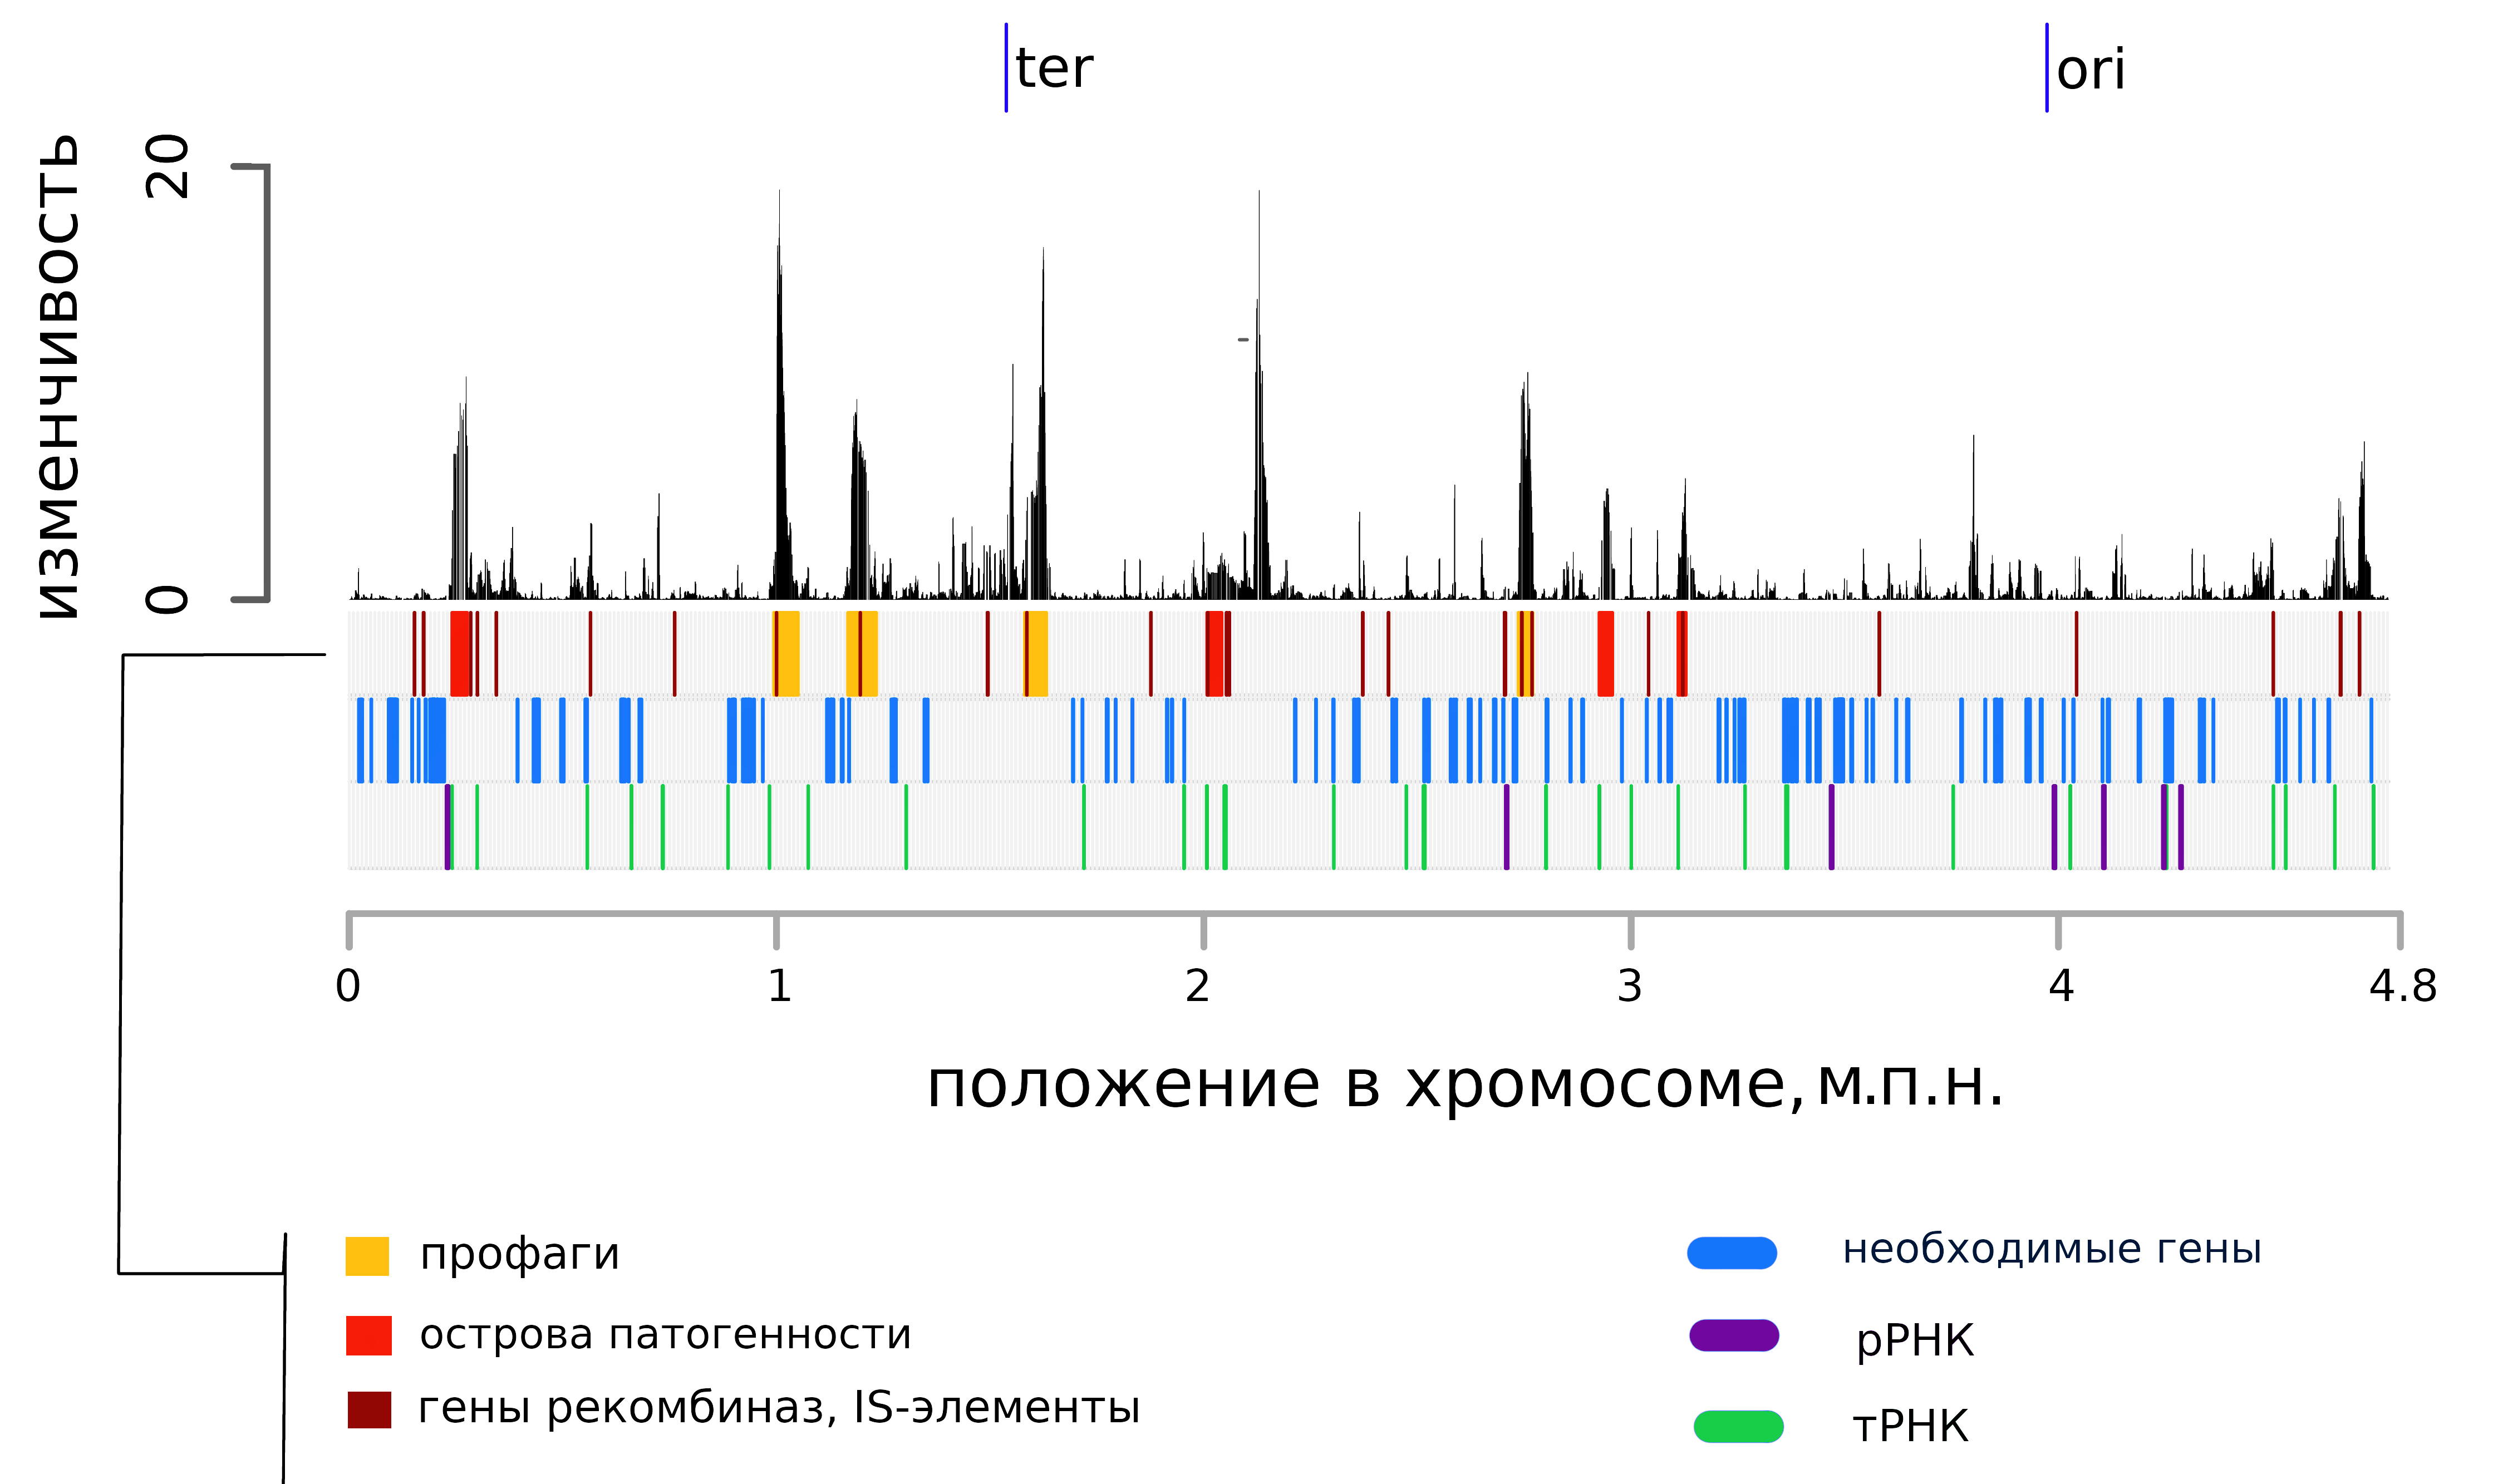
\includegraphics[width=\textwidth]{Dissertation/images/complexity/figure5plus2.png}
  \caption{Профиль вариабельности генома \textit{E. coli LF82}. Цветом обозначены острова патогенности, профаги, гены, ассоциированные с мобильными элементами генома, жизненно-необходимые гены, гены транспортных и рибосомных РНК. Области повышенной изменчивости содержат меньше жизненно-необходимых генов. Профаги и острова патогенности обладают повышенным уровнем изменчивости по сравнению с остальной частью генома.}
  \label{img:complexity_lf82} 
\end{figure}


\subsection{Сравнение профилей вариабельности филогрупп \textit{E. coli}}
Рассмотрим, как соотносятся профили изменчивости геномов из различных внутривидовых структур данного вида. Ценность подобного анализа состоит в возможности установить временную динамику "горячих"\ точек изменчивости (их устойчивость во времени). Также, подобное сравнение является еще одной проверкой предложенного метода: если у геномов из разных подвидовых структур не будет наблюдаться схожести в профиле вариабельности, то это ставит под сомнение ценность анализа для вида в целом. С другой стороны, воспроизводимость --- схожесть профилей --- будет свидетельством того, что получаемый при анализе профиль изменчивости отражает некоторый реальный биологический эффект. 

Для проведения данного анализа мы использовали геномы из пяти наиболее крупных филогрупп (A, B1, B2, D, E) \textit{E. coli}. Мы выбрали по одному референсному геному из каждой филогруппы; для каждого из референсных геномов подобрали 100 наиболее близких (по суммарной ширине выравнивания) геномов, доступных в базе RefSeq, в которой на момент проведения анализа содержалось 5466 геномов кишечной палочки; оценили профиль изменчивости внутри каждой из филогрупп независимо, используя только геномы данной филогруппы. 

\begin{figure}[!ht] 
  \center
    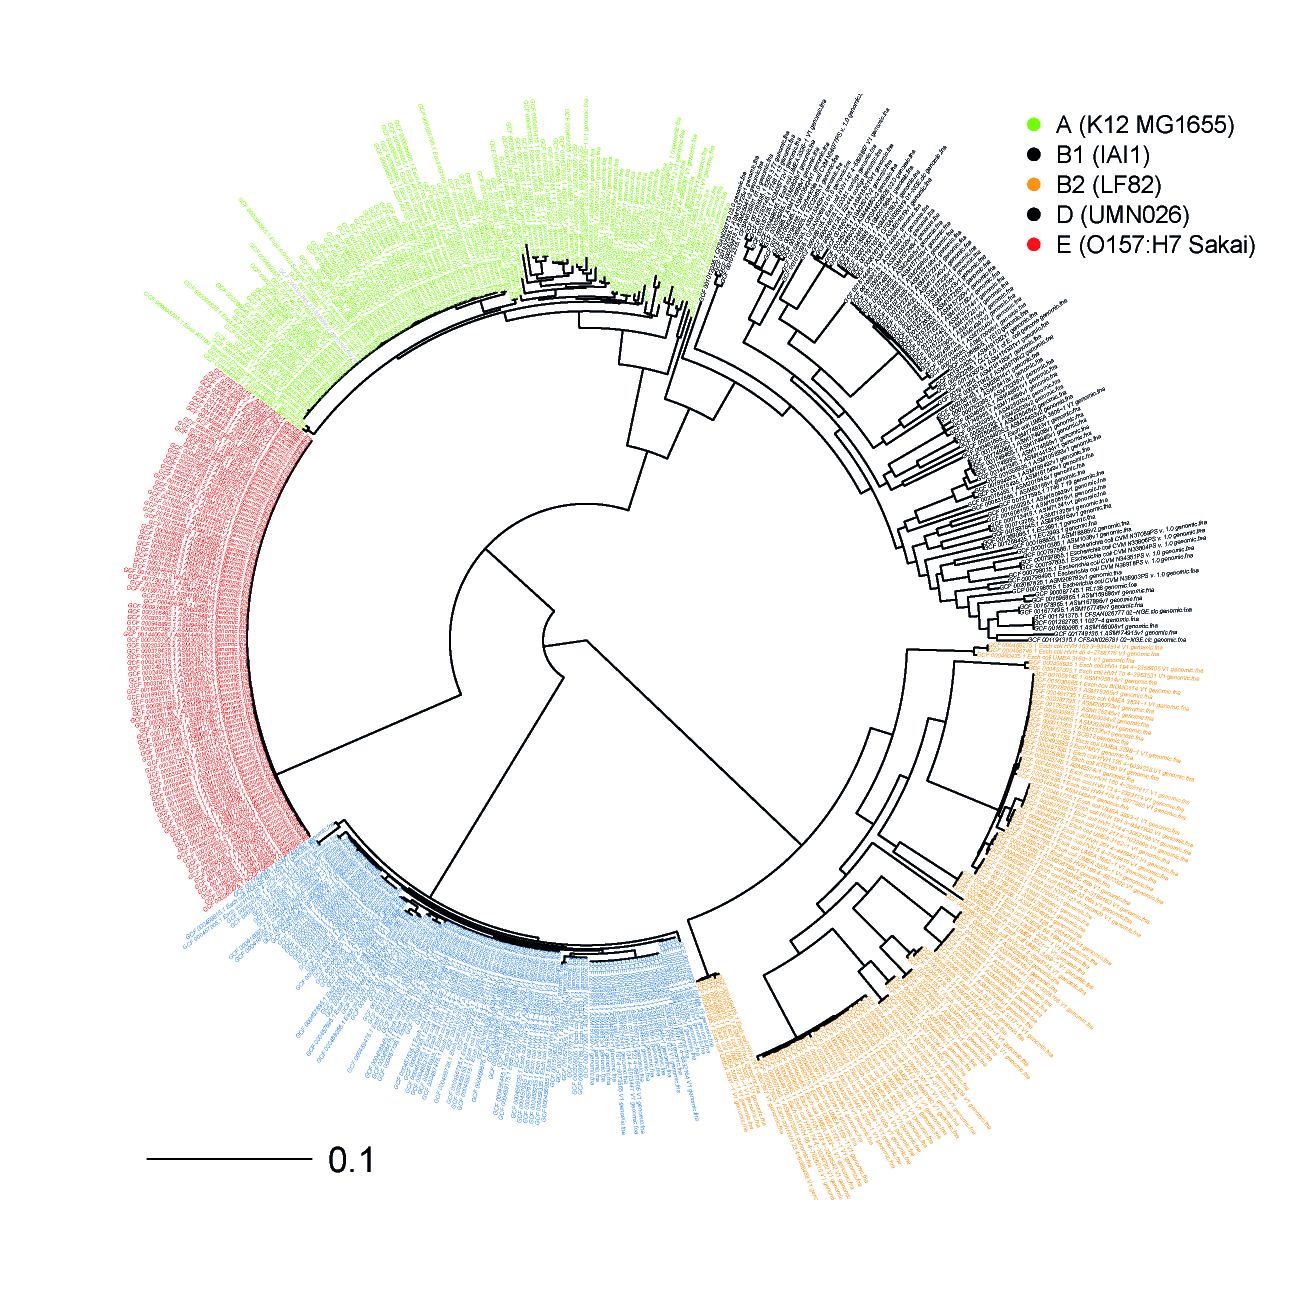
\includegraphics[width=0.65\textwidth]{Dissertation/images/complexity/coli_phylogroups.png}
  \caption{Филогенетическое дерево выборки геномов \textit{E. coli}, состоящей из представителей пяти крупных филогрупп: A, B1, B2, D, E (обозначены зеленым, черным, оранжевым, синим, красным цветом соответственно).}
  \label{img:phylogroups} 
\end{figure}

На рисунке~\ref{img:phylogroups} показано филогенетическое дерево подобранного таким образом набора геномов. На рисунке~\ref{img:phylogroups_complex} показаны профили вариабельности по пяти геномам из различных филогрупп, серым цветом обозначены блоки синтении, оранжевым - области нахождения профагов. Длины геномов значительно различаются: от 4.6 млн. п.о. в случае \textit{K12} до 5.5 м.п.н. у \textit{O157:H7 Sakai}. Профили изменчивости геномов масштабированы таким образом, чтобы они совпадали по длине на рисунке; снизу от профилей изменчивости показаны координатные оси.

\begin{figure}[!ht] 
  \center
    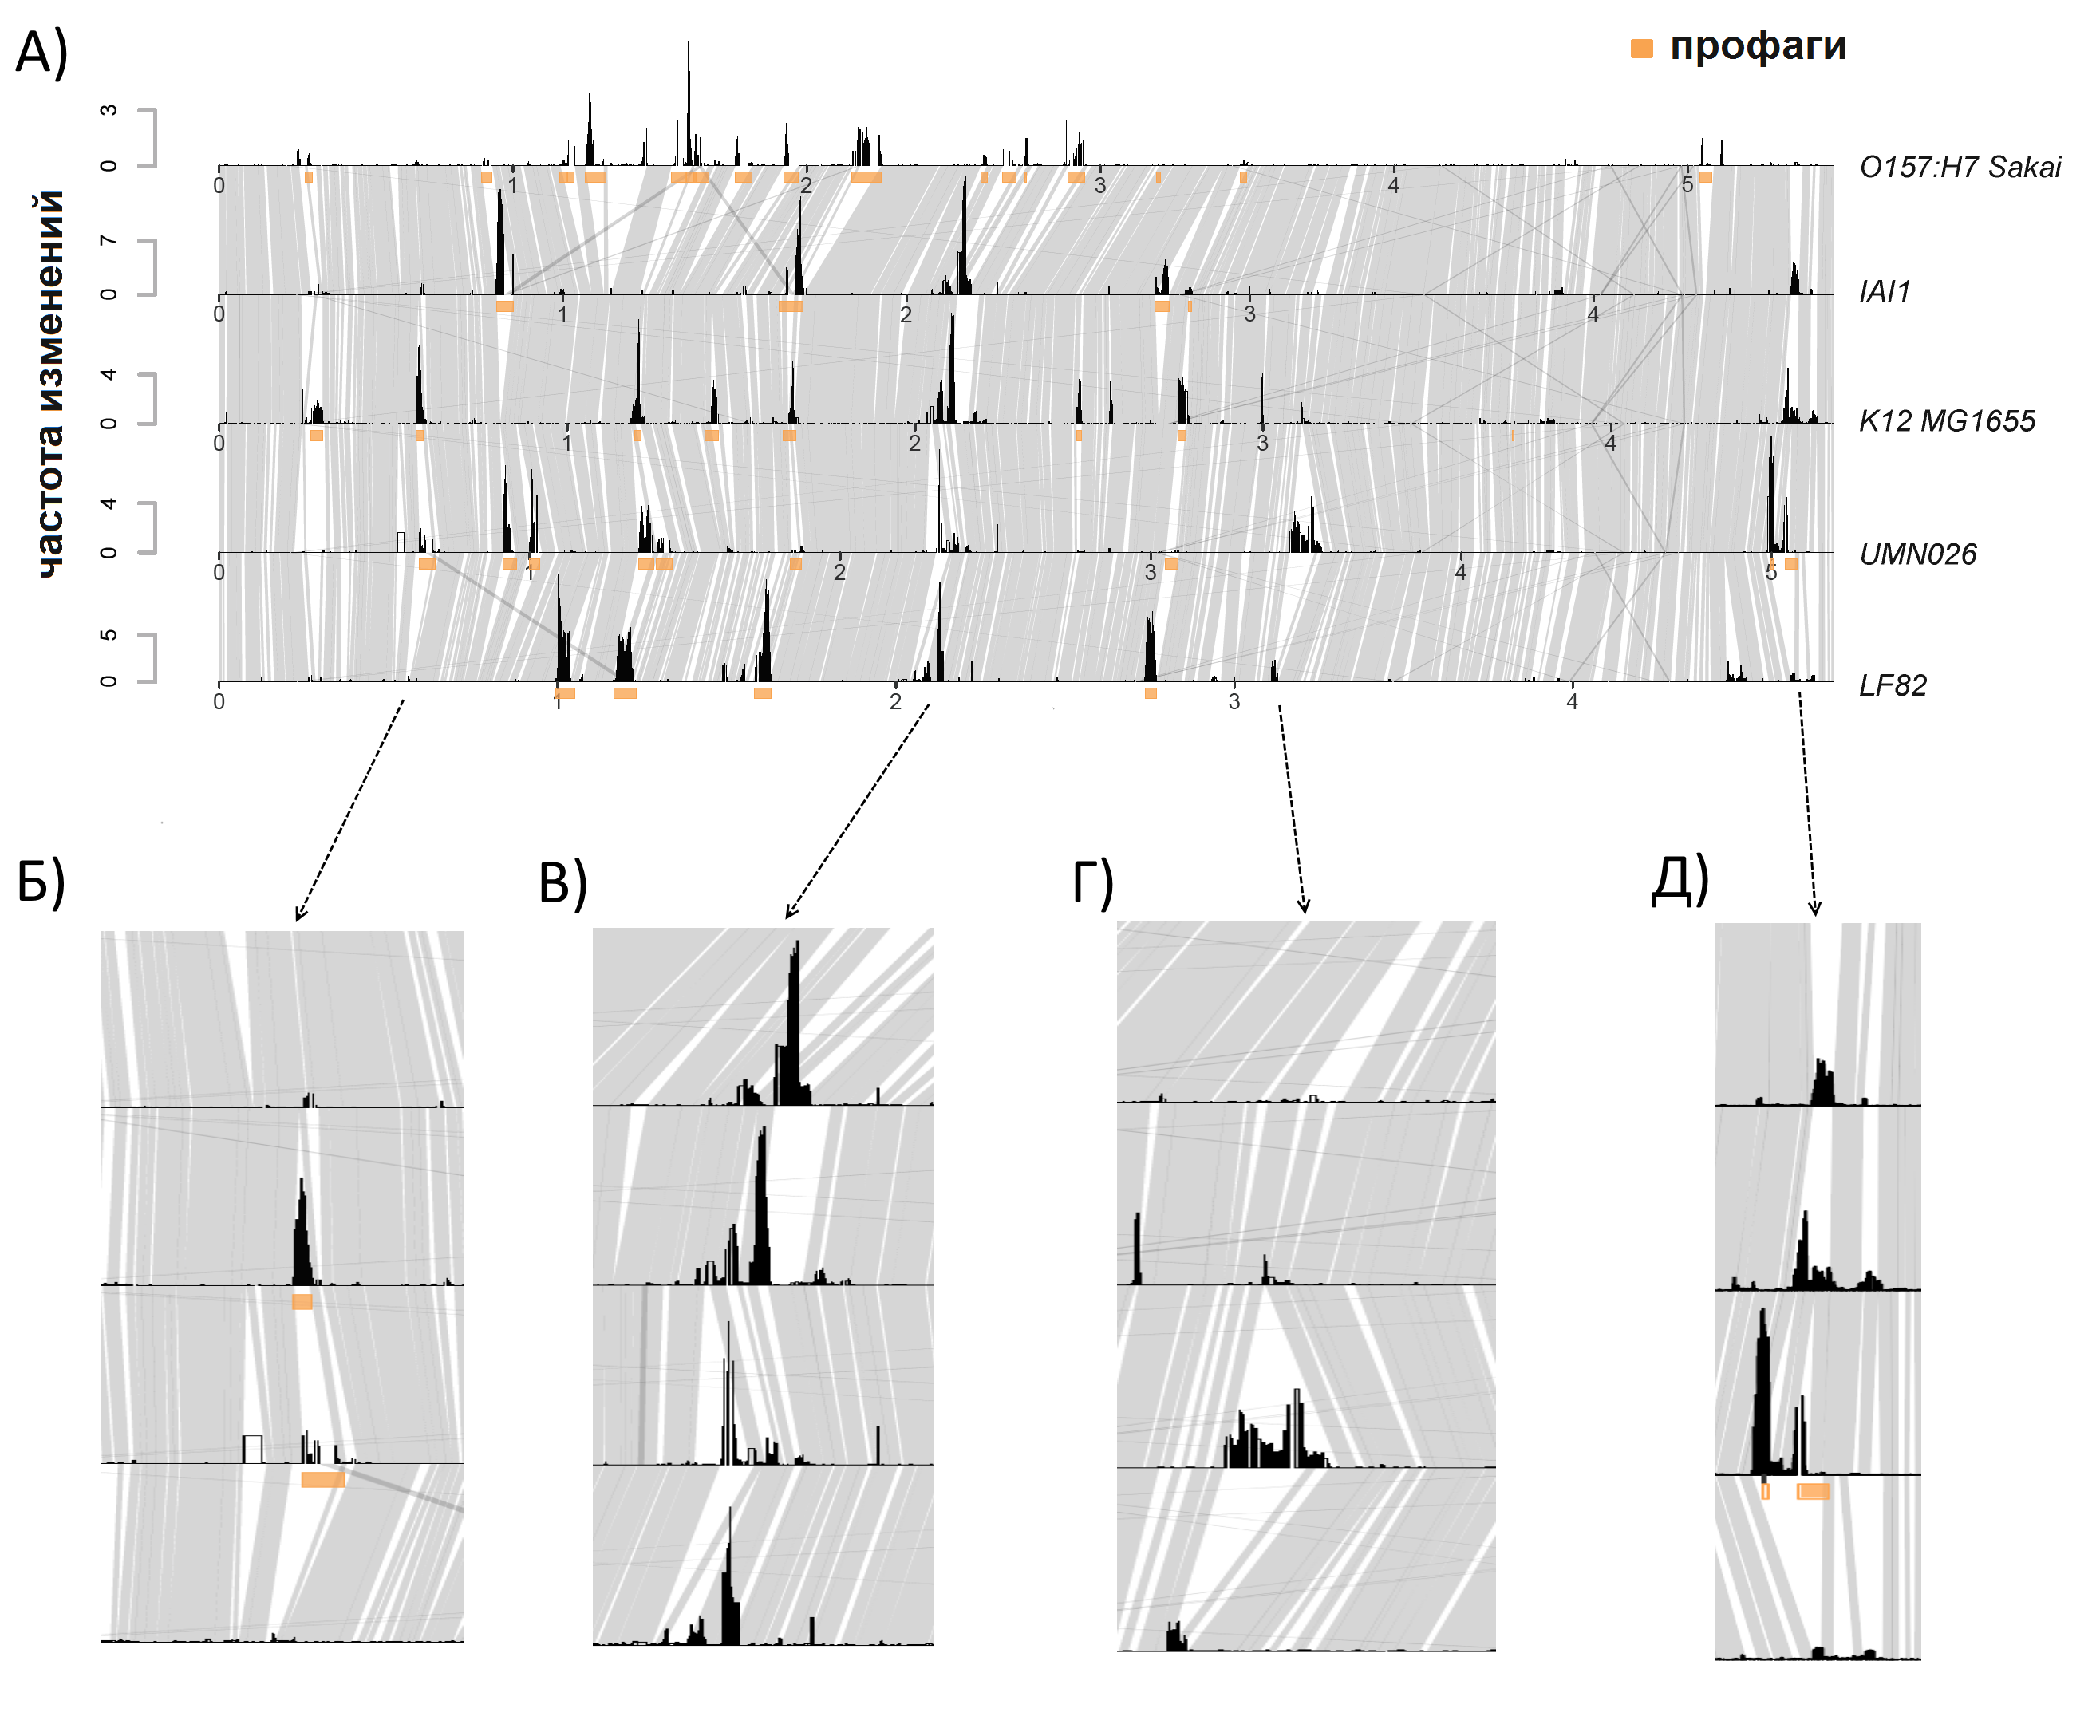
\includegraphics[width=\textwidth]{Dissertation/images/complexity/coli_phylogroups_complexity_3.png}
  \caption{Сравнение профилей вариабельности представителей пяти филогрупп \textit{E. coli LF82}. Оранжевым цветом выделены области, определенные как профаговые. Блоками серого цвета показаны блоки синтении.}
  \label{img:phylogroups_complex} 
\end{figure}

Как и в вышеописанном случае анализа 327 геномов кишечной палочки, анализ по отдельным филогруппам показывает, что большая часть областей с повышенной вариабельностью соответствует местам встройки фагов. Особенно это заметно в случае филогруппы E (штамм \textit{O157:H7 Sakai}), экспансия фагов в которой привела к значительному увеличению размера генома.   

В целом, профили обладают высокой долей сходства: значительная часть областей повышенной вариабельности сохраняет свое расположение у части, либо во всех филогруппах. Это наблюдается как для профаговых областей (рис.~\ref{img:phylogroups_complex} Б), так и для областей без признаков профагов и других мобильных элементов (рис.~\ref{img:phylogroups_complex} В). Горячие точки могут иметь различную степень изменчивости в разных филогруппах (рис.~\ref{img:phylogroups_complex} Б, Г, Д).

Заметно существование "холодных"\ областей генома, обладающих низкой вариабельностью во всех филогруппах. Длина этих низко-вариабельных участков может значительно превышать характерные длины оперонов, и достигать величин порядка миллиона пар оснований (например, область в окрестности 4 млн. п.о. на рисунке~\ref{img:phylogroups_complex} А.

\subsection{Сравнение профилей вариабельности филогрупп у других видов}

В данном разделе мы приводим результаты сравнения профилей изменчивости для филогрупп у других видов бактерий. Мы рассмотрели филогруппы двух видов рода \textit{Pseudomonas} (\textit{P. aeruginosa} и \textit{P. fluorescens}), один из этих видов является естественно-компетентным, а также у \textit{Neisseria gonorrhoeae} - также естественно компетентного вида, для которого характерна высокая частота рекомбинационных событий \cite{yu2014genome}.

\textit{Pseudomonas} - род грамотрицательных бактерий, отдельные виды которого значительно различаются по метаболическому потенциалу и занимаемым экологическим нишам. \textit{P. fluorescens} обитают преимущественно в почве и являются естественно компетентными. \textit{P. aeruginosa} - оппортунистические патогены человека, для которых компетентность наблюдалась лишь в условиях жизни в биопленке \cite{nolan2019pseudomonas}. На рисунке~\ref{img:pseudo_phylogroups} показаны филогенетические деревья для двух видов, цветом выделены клады дерева, отобранные для оценки и сравнения профилей изменчивости. Для \textit{P. fluorescens} в первой кладе было 95 генома, и 115 геномов --- во второй; для \textit{P. fluorescens} в первой кладе было 73 генома и 143 генома --- во второй.

\begin{figure}[!ht] 
  \center
    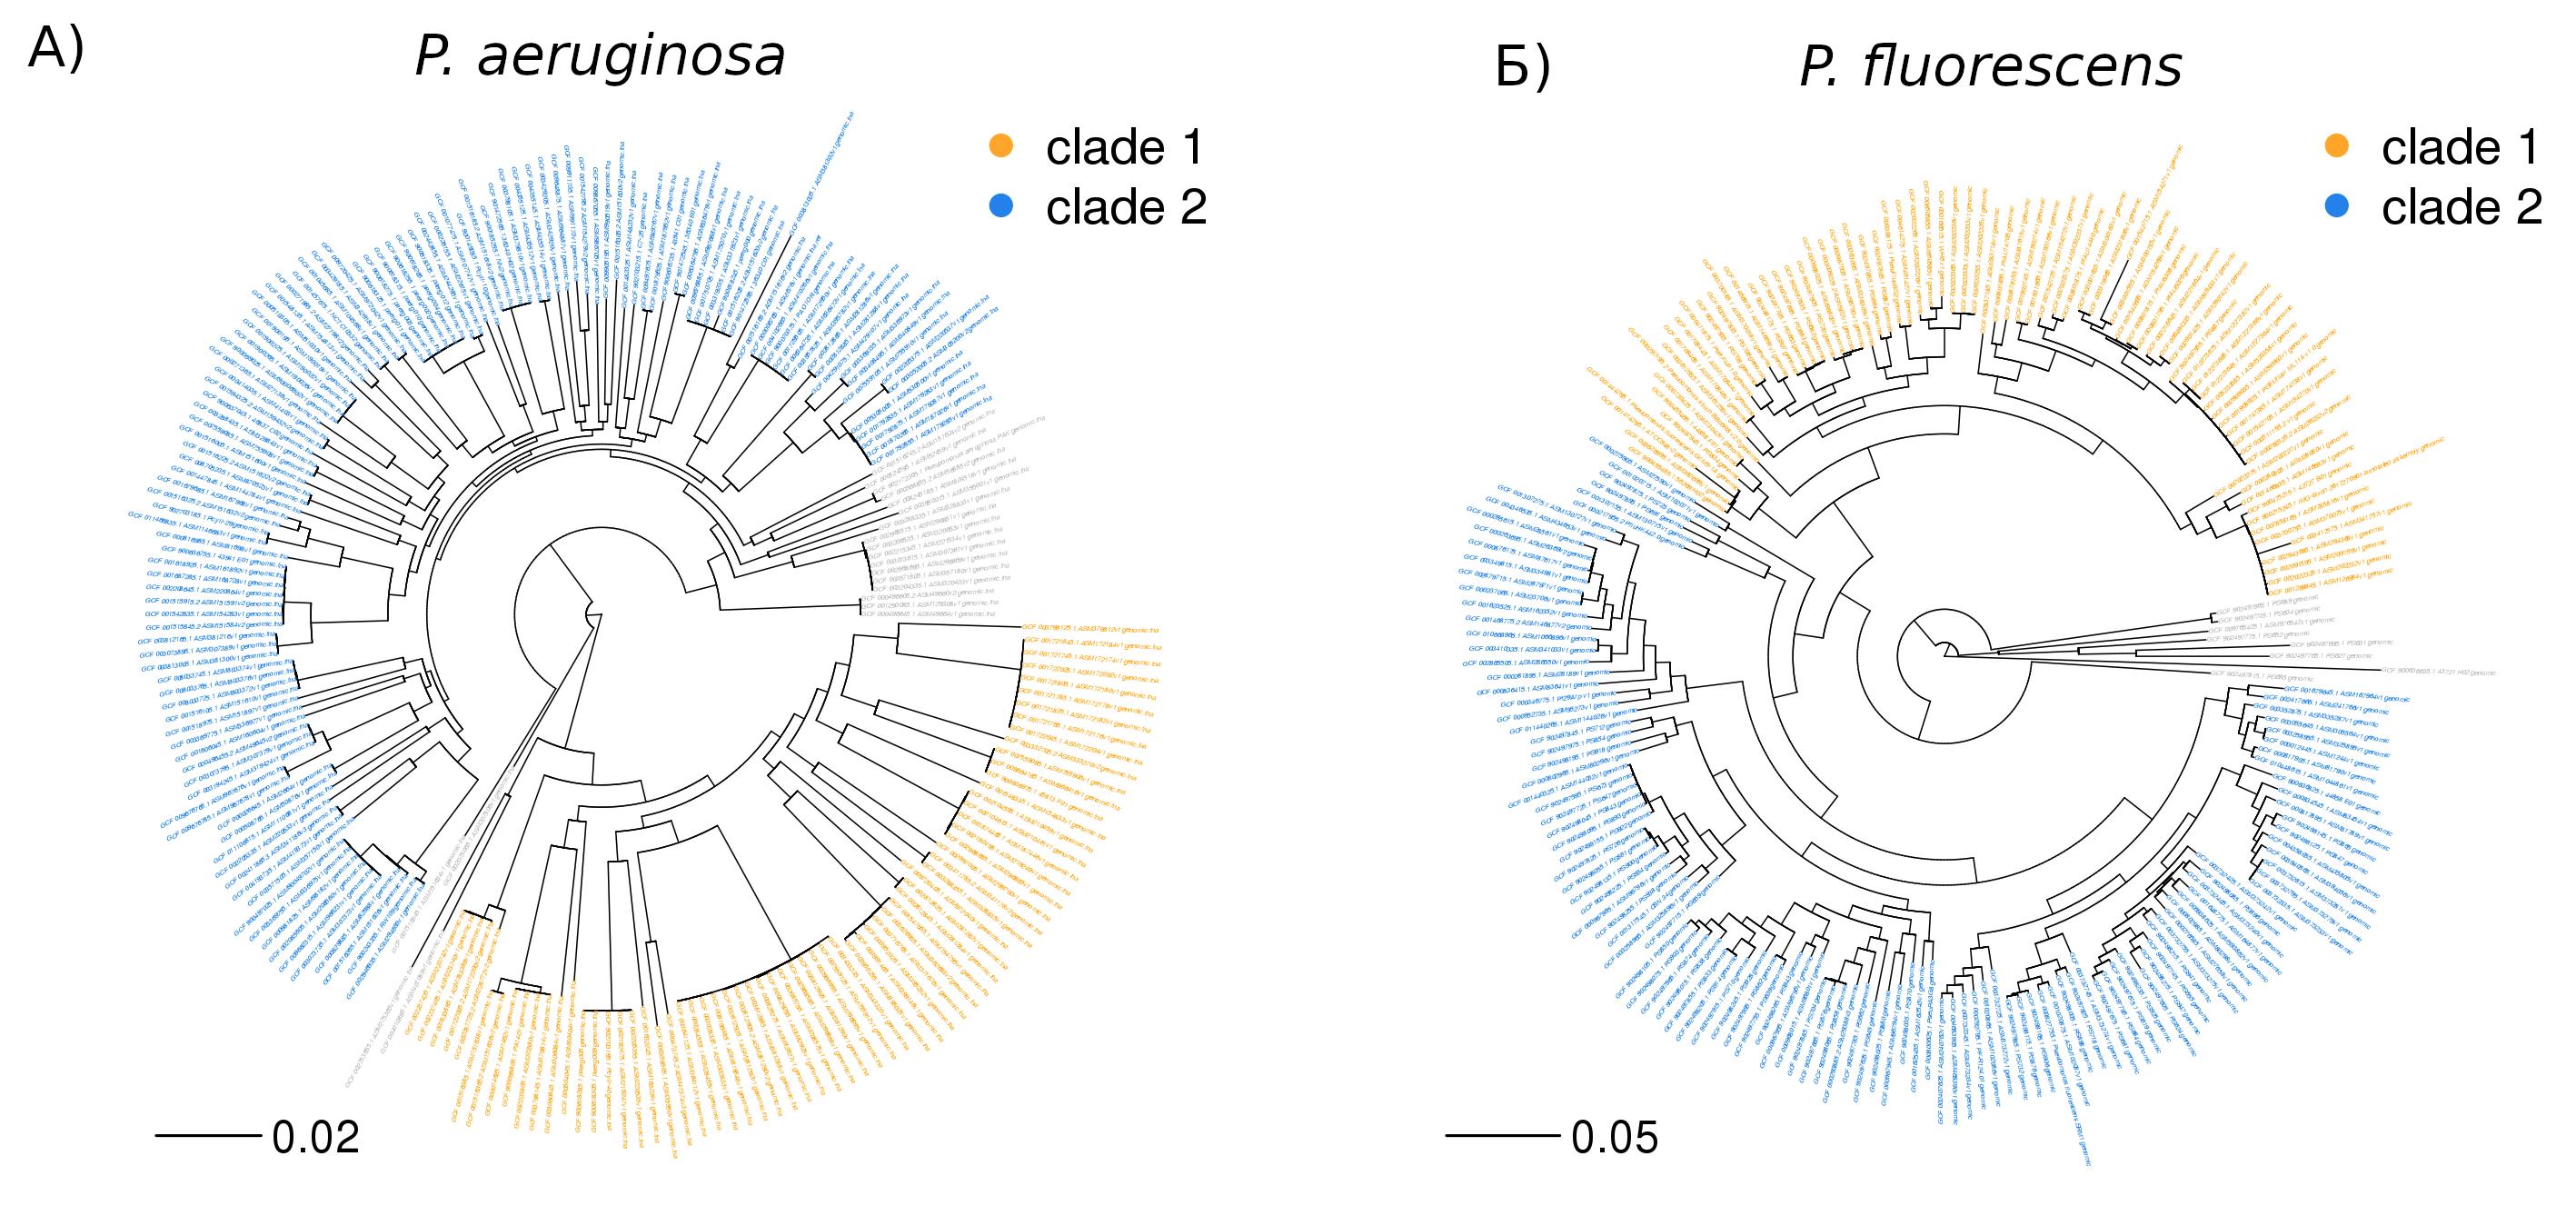
\includegraphics[width=\textwidth]{Dissertation/images/complexity/pseudo_phylogroups.png}
  \caption{Филогенетическое дерево геномов видов: А) \textit{P. aeruginosa} и Б) \textit{P. fluorescens}. Оранжевым и синим цветом выделены клады дерева, отобранные для анализа профилей изменчивости. }
  \label{img:pseudo_phylogroups} 
\end{figure}

На рисунке~\ref{img:pseudo_complexity} показано сравнение профилей изменчивости, оцененных независимо для геномов из различных клад филогенетического дерева. В случае \textit{P. aeruginosa}, подобно \textit{E. coli}, наблюдается значительное сходство профилей изменчивости геномов в двух филогенетических кладах (рис. ~\ref{img:pseudo_complexity} А). В случае \textit{P. fluorescens} подобное сходство выражено слабо и заметно только в небольшом фрагменте ближе к концу хромосомы, после 6 млн. пар оснований, а сами профили вариабельности более равномерны и обладают меньшим количеством выраженных горячих точек (рис. ~\ref{img:pseudo_complexity} Б). Вероятная причина наблюдаемой разницы - высокая частота крупных хромосомных перестроек у \textit{P. fluorescens} (заметно, в том числе, по визуализации блоков синтении). Частые хромосомные перестройки делают анализ локальной изменчивости мало информативным, для применимости метода необходимо: во-первых, наличие локальных участков повышенной изменчивости, и во-вторых, чтобы глобальные перестройки хромосомы происходили сравнительно редко относительно локальных изменений (вставки, делеции и транслокации отдельных генов).

\begin{figure}[!ht] 
  \center
    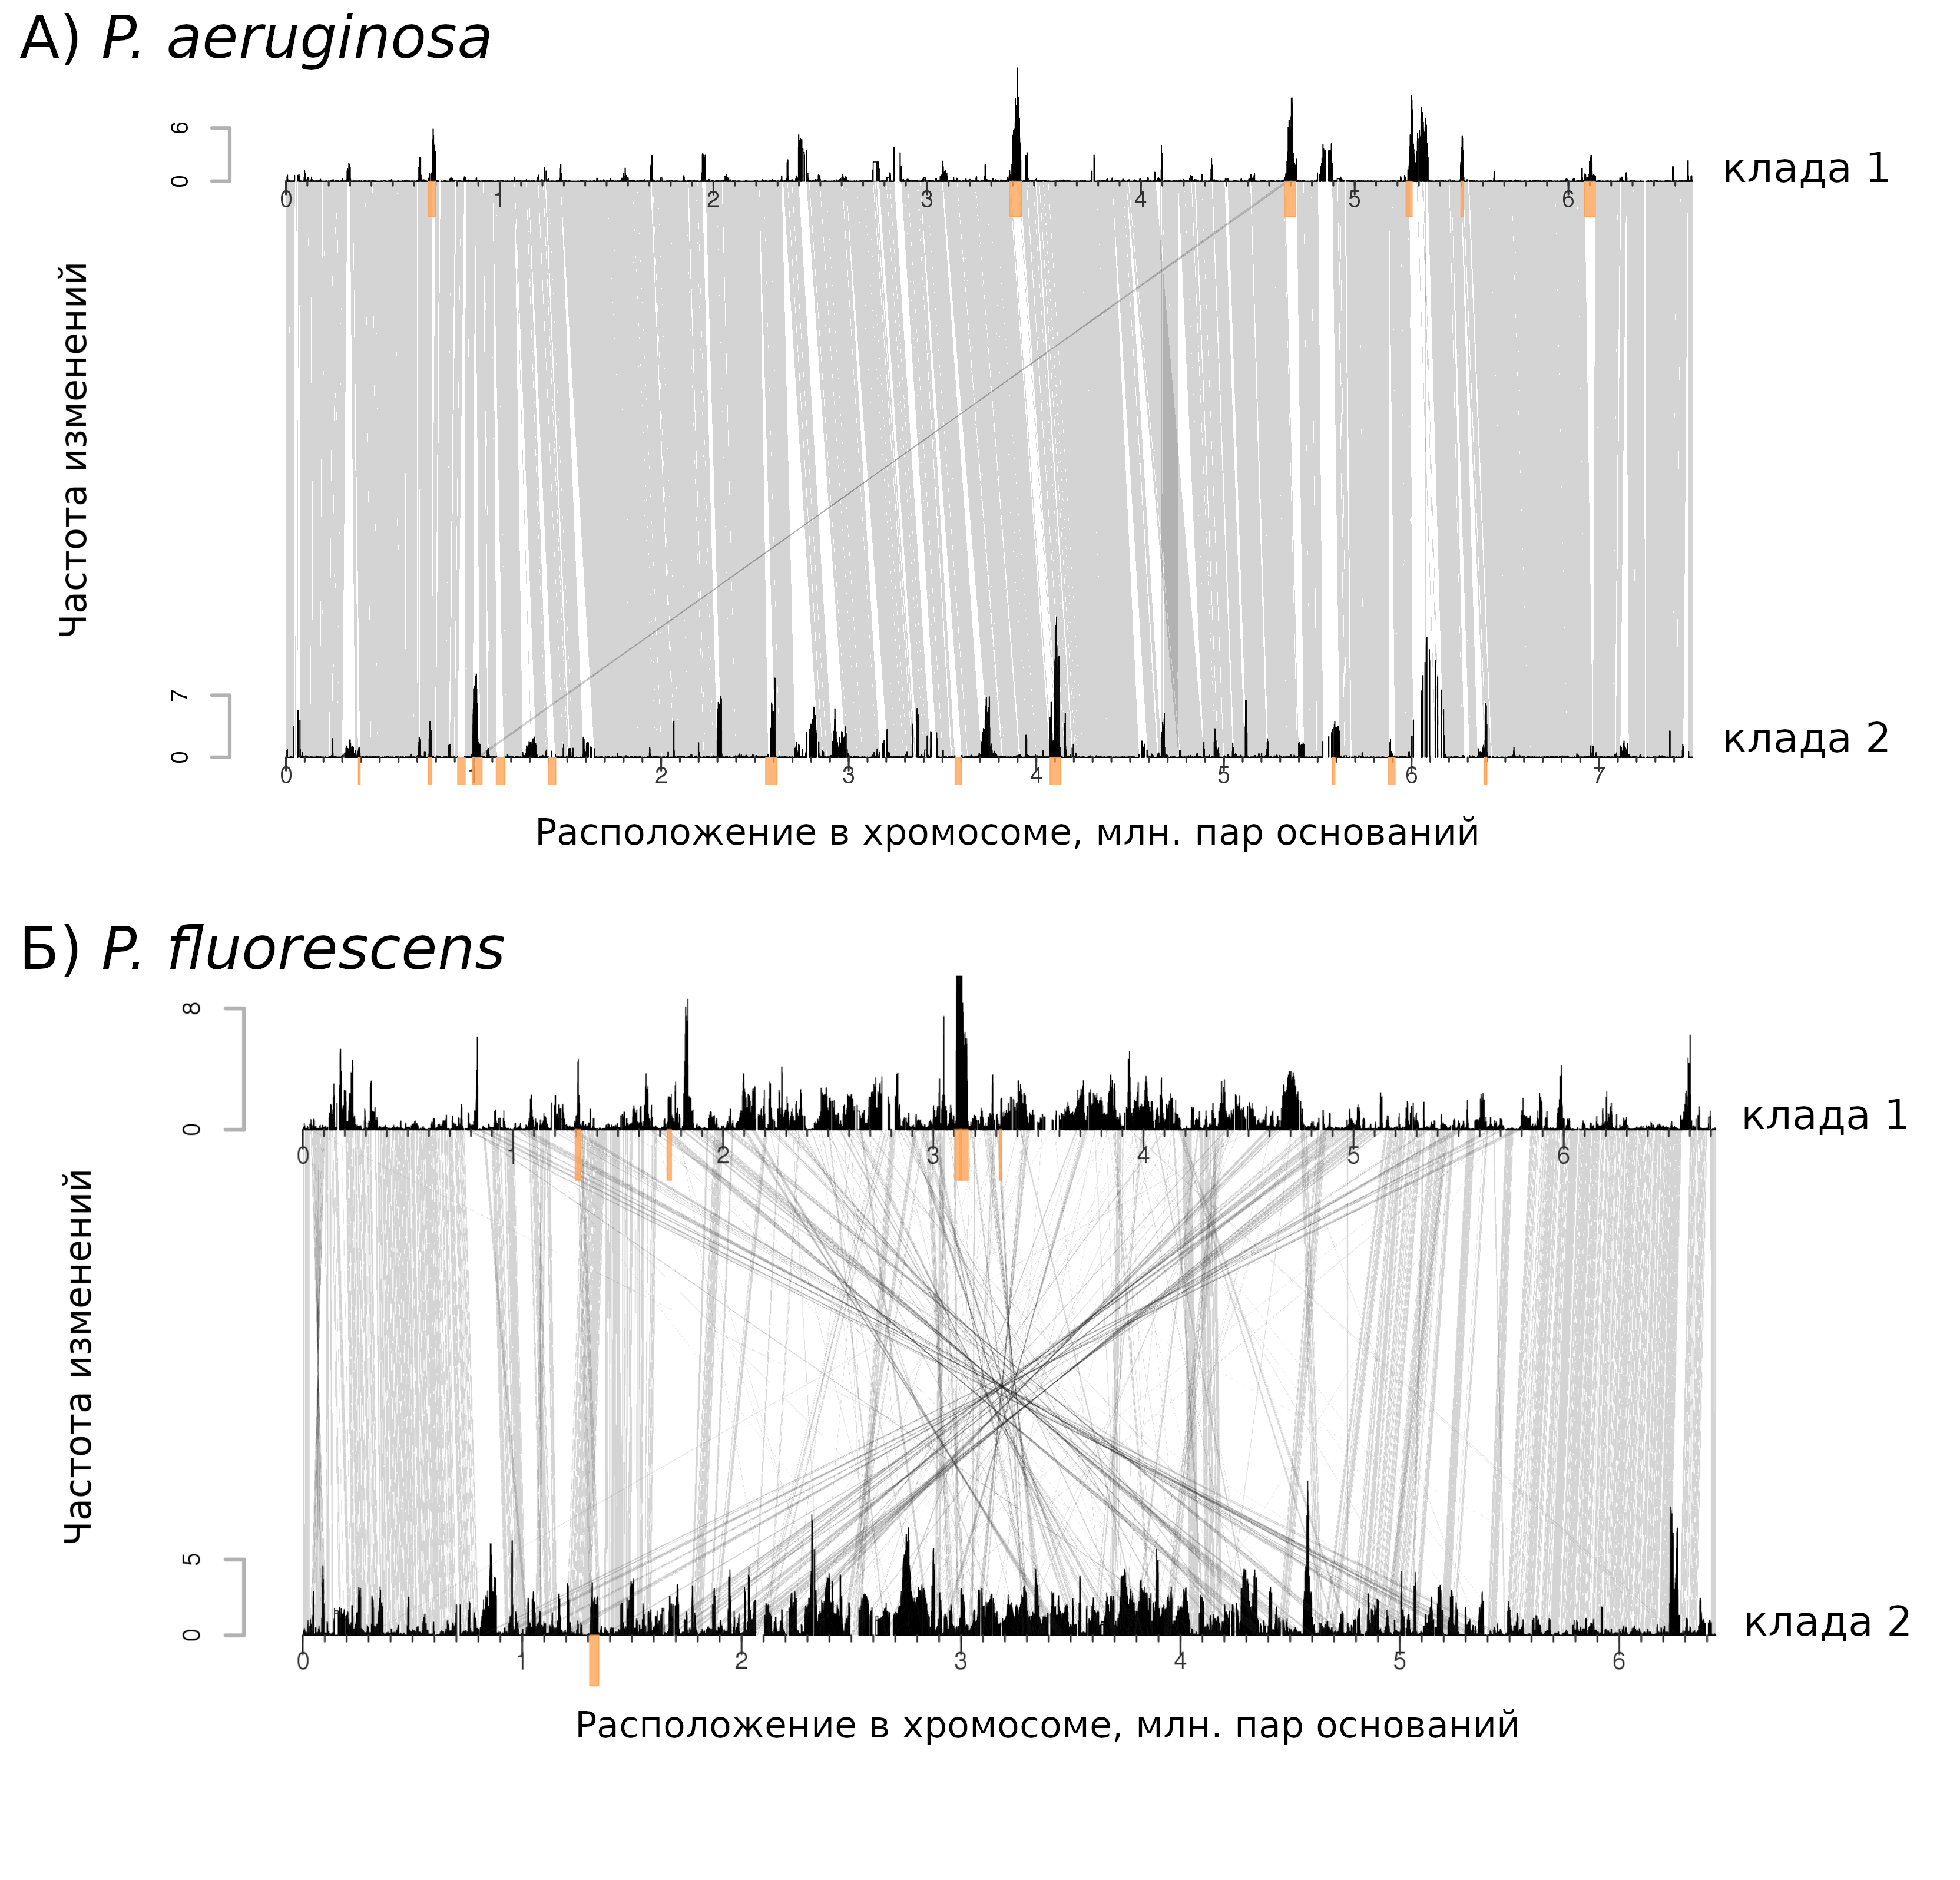
\includegraphics[width=\textwidth]{Dissertation/images/complexity/pseudo_complexity.png}
  \caption{Сравнение профилей вариабельности двух клад вида  А) \textit{P. aeruginosa} и Б) \textit{P. fluorescens}. Оранжевым цветом выделены области, определенные как профаговые.}
  \label{img:pseudo_complexity} 
\end{figure}

Для \textit{N. gonorrhoeae} мы рассмотрели 4 клады. Количество геномов составило 49, 51, 47 и 75 геномов для первой, второй, третьей и четвертой клады, соответственно. Профили геномов из различных клад филогенетического дерева у обладают выским уровнем сходства (рис~\ref{img:ghono_complex}).

\begin{figure}[!ht] 
  \center
    \subcaptionbox{}{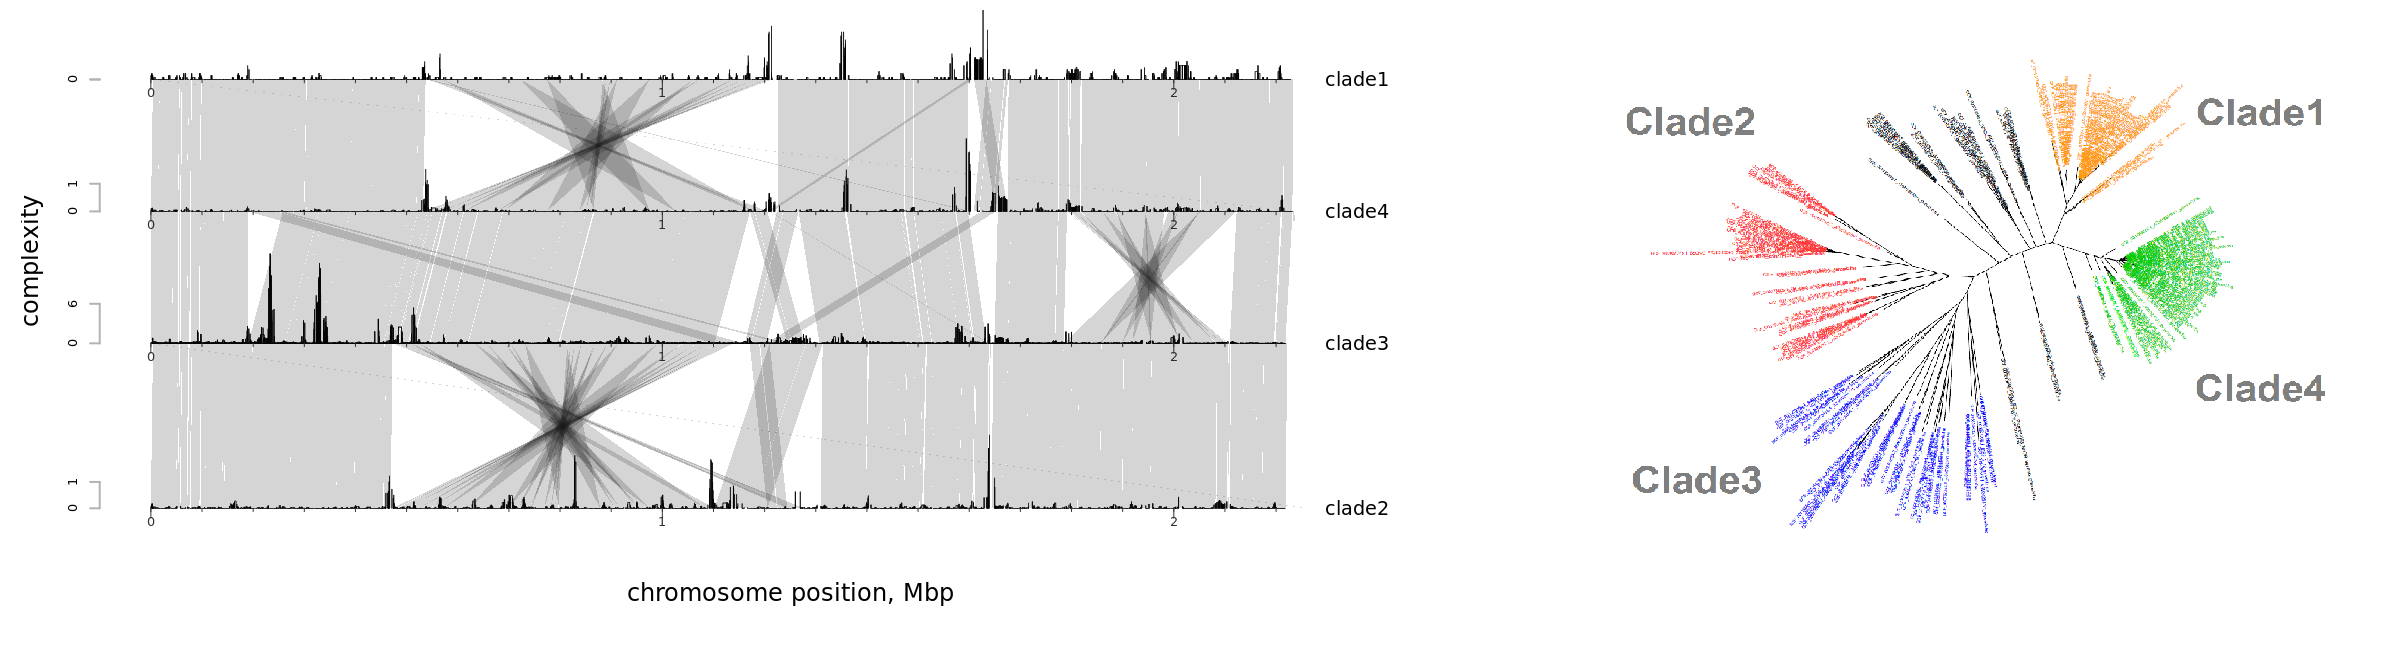
\includegraphics[width=0.6\textwidth]{Dissertation/images/complexity/neisseria_clades.png}}
    \subcaptionbox{}{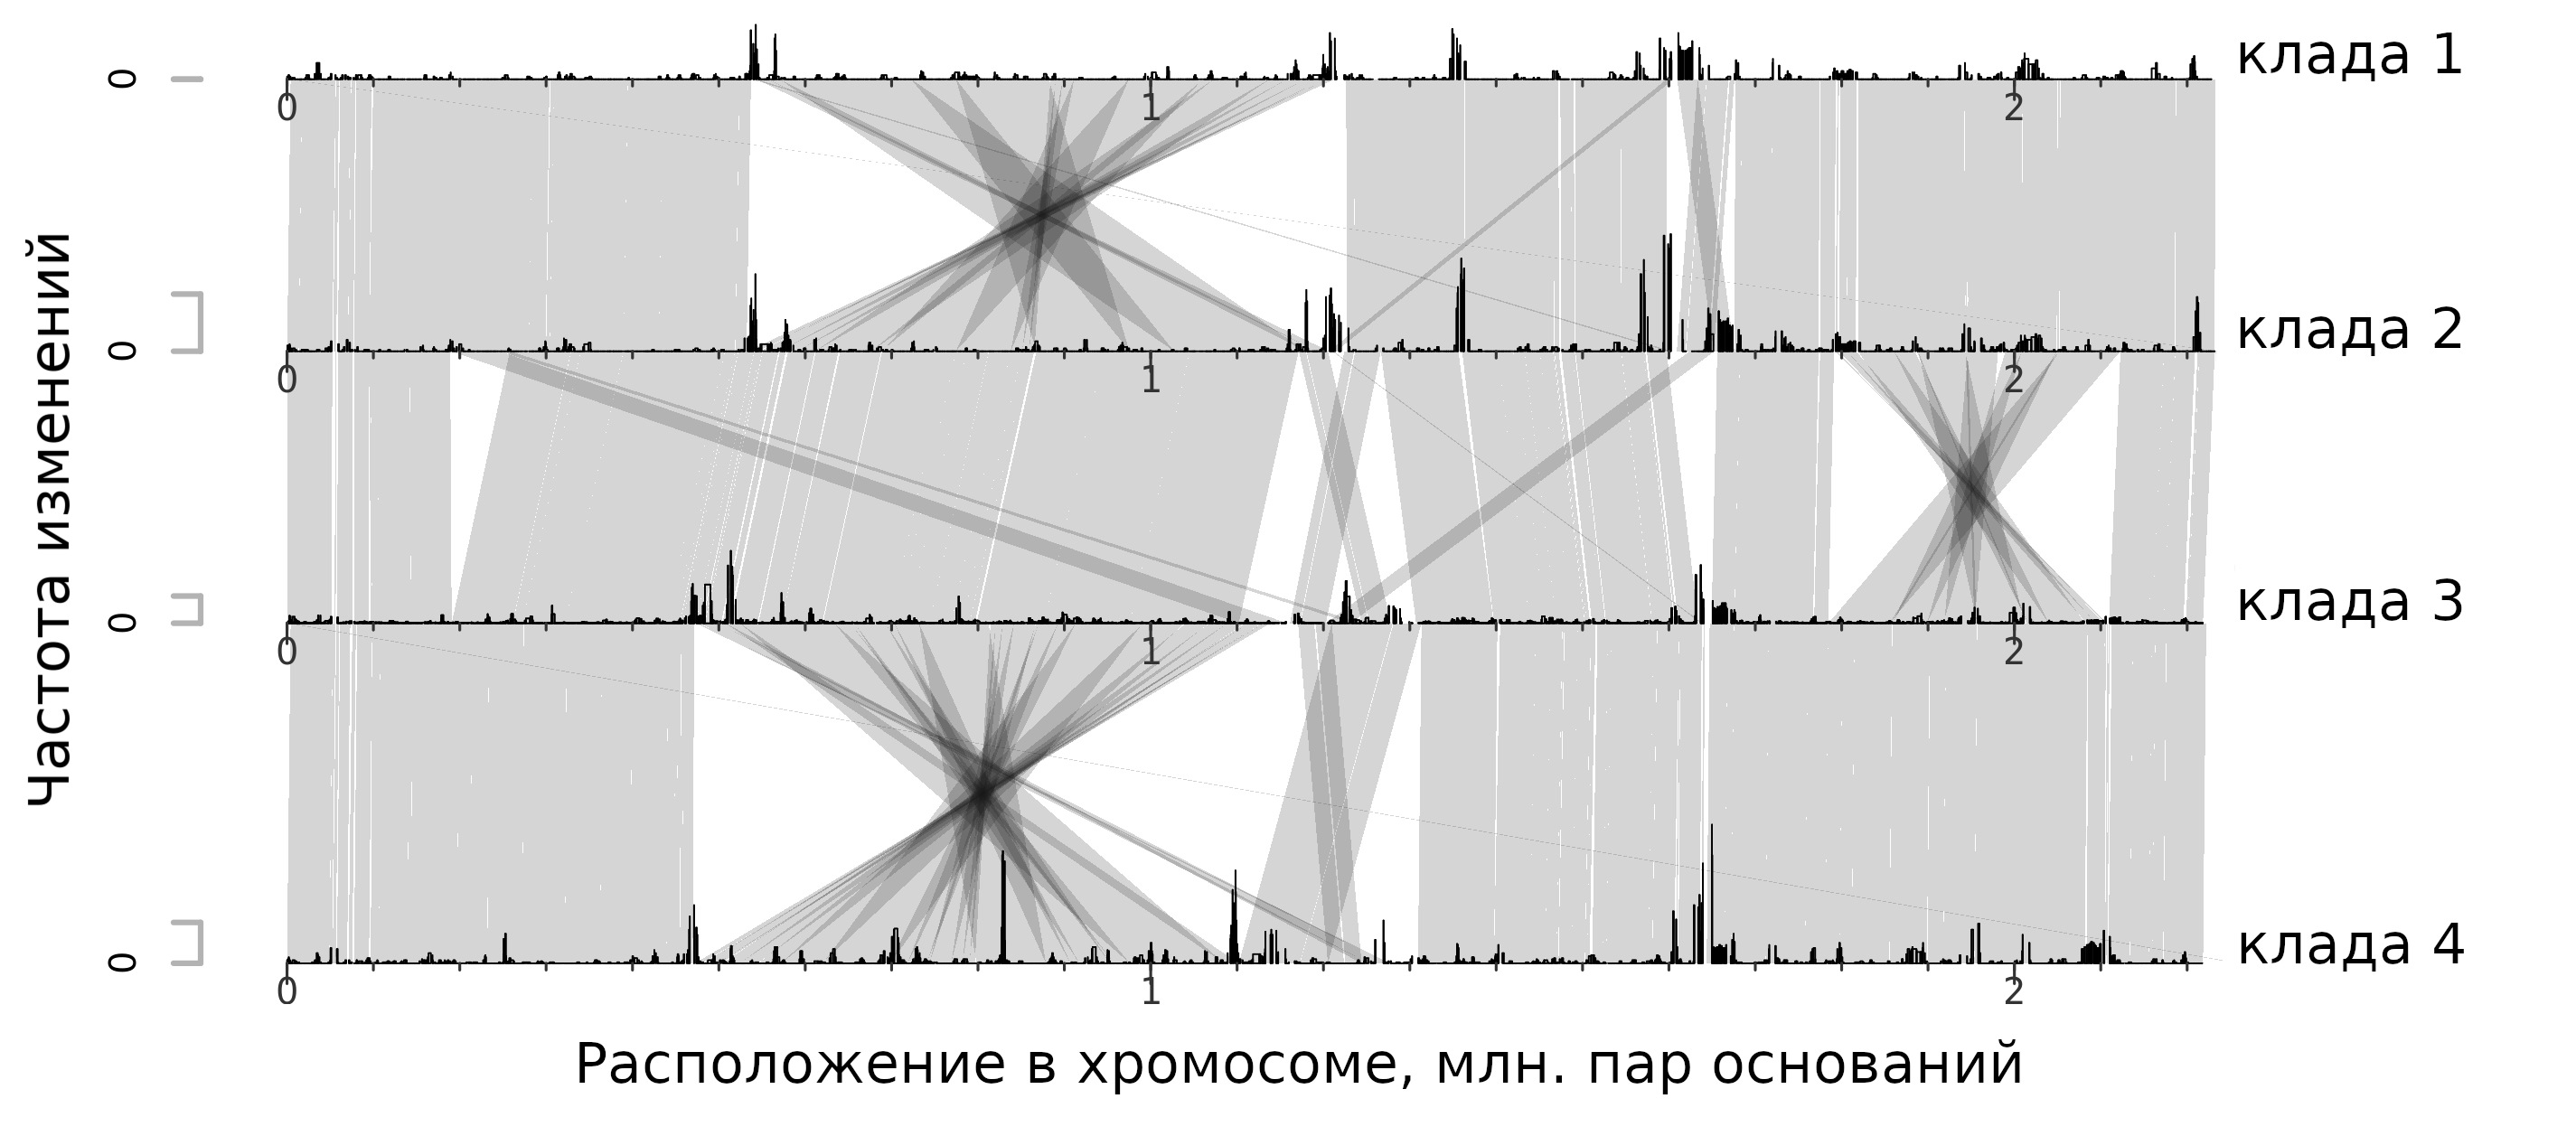
\includegraphics[width=\textwidth]{Dissertation/images/complexity/neisseria_ghono.png}}
  \caption{Сравнение профилей вариабельности четырех филогенетических клад вида \textit{N. gonorrhoeae}. А) Филогенетическое дерево с указанием выбранных клад. Б) сравнение профилей вариабельности.}
  \label{img:ghono_complex} 
\end{figure}

\subsection{Сравнение профилей вариабельности между близкородственными видами}

\begin{figure}[!ht] 
  \center
    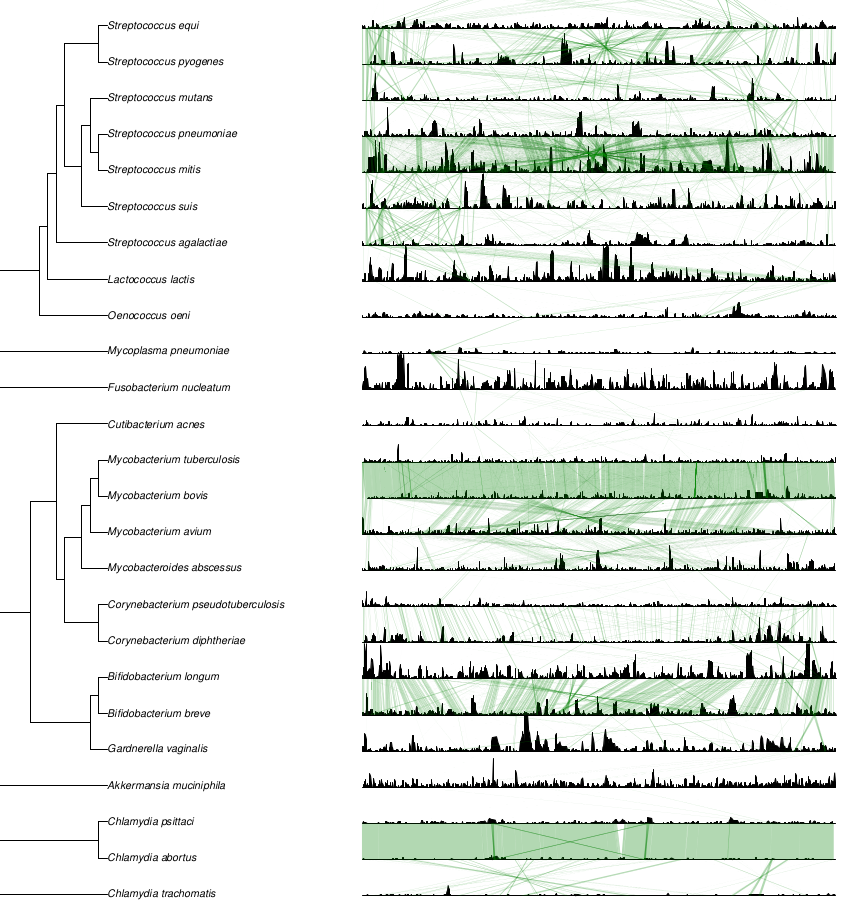
\includegraphics[width=\textwidth]{Dissertation/images/complexity/tree_fragment.png}
  \caption{Фрагмент визуализации профилей изменчивости геномов различных видов. Профили расположены в соответствии с филогенетическим деревом видов, блоки синтении показаны для смежных по дереву видов.}
  \label{img:tree_fragment} 
\end{figure}


\begin{figure}[!ht] 
  \center
    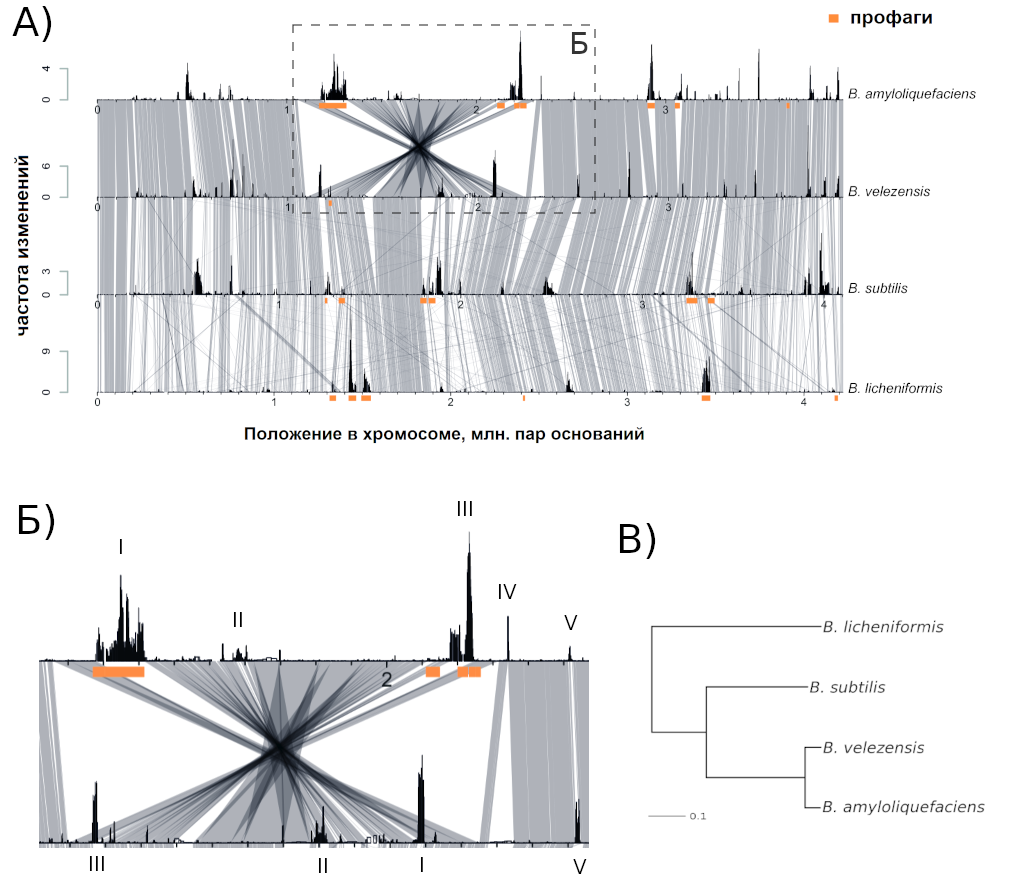
\includegraphics[width=\textwidth]{Dissertation/images/complexity/bacillus_compare_v3.png}
  \caption{Сравнение профилей вариабельности четырех различных видов рода \textit{Bacillus}. А) Профили изменчивости и блоки синтении, оранжевым цветом выделены области, определенные как профаговые, рамка из штрихованных линий показывает фрагмент, представленный на Б). В) Филогенетическое дерево рассматриваемых видов.}
  \label{img:species_complex_bacillus} 
\end{figure}


\begin{figure}[!ht] 
  \center
     \subcaptionbox{}{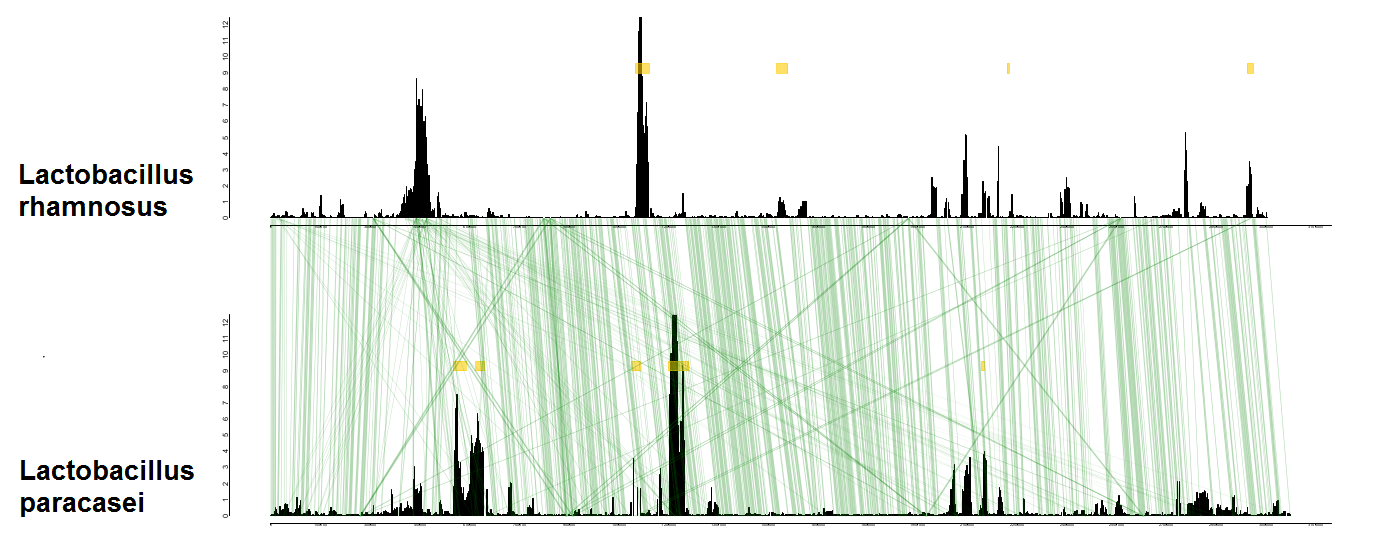
\includegraphics[width=\textwidth]{Dissertation/images/complexity/lacto_complexity.png}}
     \subcaptionbox{}{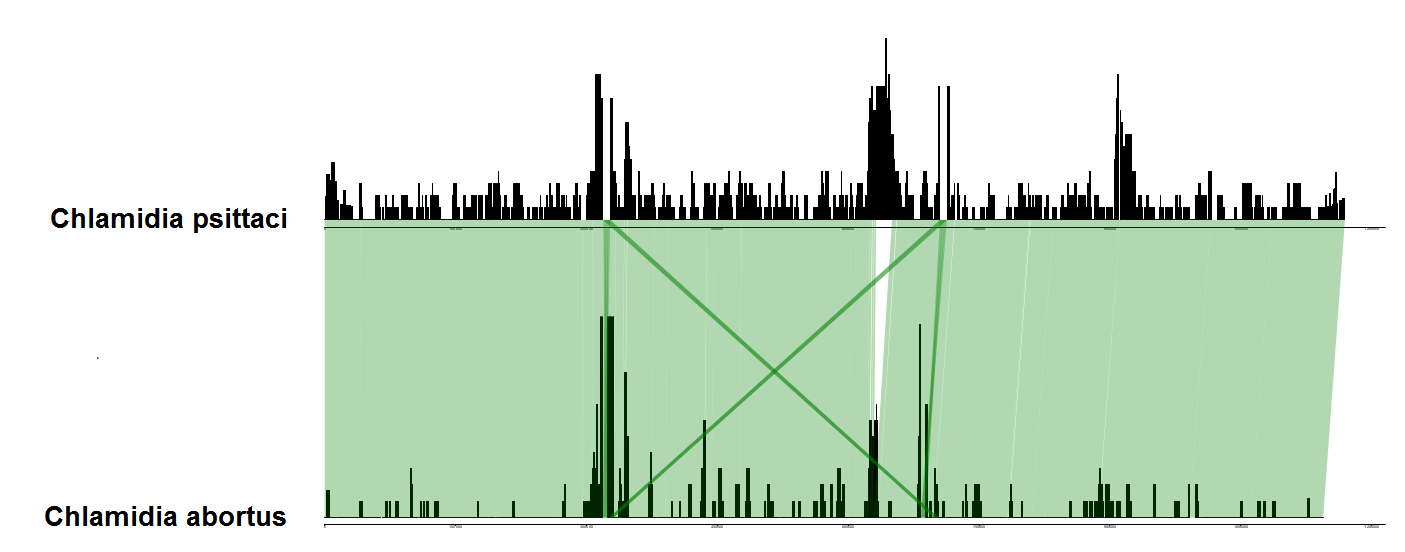
\includegraphics[width=\textwidth]{Dissertation/images/complexity/chlamidia_complexity.png}}
  \caption{Сравнение профилей вариабельности для: А) двух видов рода \textit{Lactobacillus}, Б) двух видов рода \textit{Chlamidia}. Оранжевым цветом выделены области, определенный как профаговые.}
  \label{img:species_complex_lactobacillus_chlam} 
\end{figure}

Внутри вида профили изменчивости обладают высокой степенью сходства. Для выяснения степени сходства профилей изменчивости для геномов из разных видов, мы провели анализ изменчивости у 143 видов бактерий и архей. В рассмотрение мы брали те виды, для которых было доступно как минимум 50 геномов на момент начала анализа (2016 год). Визуализация профилей доступна на веб-сервере \url{gcb.rcpcm.org}, о котором будет подробнее рассказано ниже. Все профили изменчивости были расположены в соответствии с филогенетическим деревом, блоки синтении рассчитывались между всеми парами видов, расположенными последовательно на дереве. Фрагмент итоговой визуализации показан на рисунке~\ref{img:tree_fragment}, полная визуализация доступна по адресу \url{https://github.com/paraslonic/GCB_revision/blob/master/figures/S3_Fig.pdf}. 

В большинстве случаев, когда между видами наблюдается малое количество геномных перестроек, профили изменчивости похожи (горячие точки находятся в схожем окружении). Ниже, для примера, мы приводим отдельные сравнения профилей изменчивости.

На рисунке~\ref{img:species_complex_bacillus} А показано сравнение профилей изменчивости четырех видов рода \textit{Bacillus}, филогенетическое дерево для рассмотренных видов показано на рисунке~\ref{img:species_complex_bacillus} В. У геномов видов \textit{B. amyloliquefaciens} и \textit{B. velezensis} заметна крупная инверсия (рис.~\ref{img:species_complex_bacillus} А, выделена рамкой), при этом, области высокой изменчивости сохранили свою активность  (рис~\ref{img:species_complex_bacillus} Б, пики изменчивости обозначены римскими цифрами). 

На рисунке~\ref{img:species_complex_lactobacillus_chlam} показано сравнение профилей изменчивости для двух видов лактобацилл и двух видов хламидий.



%\subsection{Разные виды имеют разный характер распределения интенсивности вариабельности вдоль генома}

%Рассмотрим сравнение профилей вариабельности посчитанных для множества различных видов. Как видно из рисунка ...




% ################################################################### HIC 
\section{Связь между уровнем изменчивости и характеристиками генома}\label{chaptComplexWithSMTH}

Профили изменчивости для геномов из различных филогрупп и близкородственных видов показали значительную степень сходства: наблюдается множество "горячих"\ точек изменчивости со стабильным положением в хромосоме. Открытым остается вопрос о причинах этого постоянства положения зон вариабельности, а также факторов определяющих их возникновение, рост либо снижение активности. Ниже мы приводим результаты сравнения между профилем изменчивости и расположением сайтов Chi, а также частотой межхромосомных контактов. 

\subsection{Связь с распределением сайтов Chi.}
Процесс горизонтального переноса генов подразумевает проведение одного из типов рекомбинации. Как было отмечено в обзоре литературы, у бактерии \textit{E. coli} описаны сайты Chi, играющие важную роль в инициации процесса гомологичной рекомбинации. 
На рисунке~\ref{img:chi_lf82} А показан уровень локальной вариабельности и локализация сайтов Chi для хромосомы штамма \textit{E. coli LF82}. Из приведенного рисунка видно неравномерное распределение сайтов Chi по реплихорам хромосомы и их сниженная представленность в местах локализации профагов/островов патогенности, а также в областях с высокой вариабельностью. На рисунке~\ref{img:chi_lf82} б) показано сравнение уровня вариабельности и расстояний до ближайшего сайта Chi (на соответствующей цепи, лидирующей для правой реплихоры, и отстающей - для левой). Корреляция между уровнем вариабельности и расстоянием до ближайшего сайта Chi значима (p-value < 1e-16), но значение коэффициента корреляции невелико и составляет 0.25.
% code: /data11/bio/operonTravel/coli/chi/ver3
\begin{figure}[!ht] 
  \center
    \subcaptionbox{}{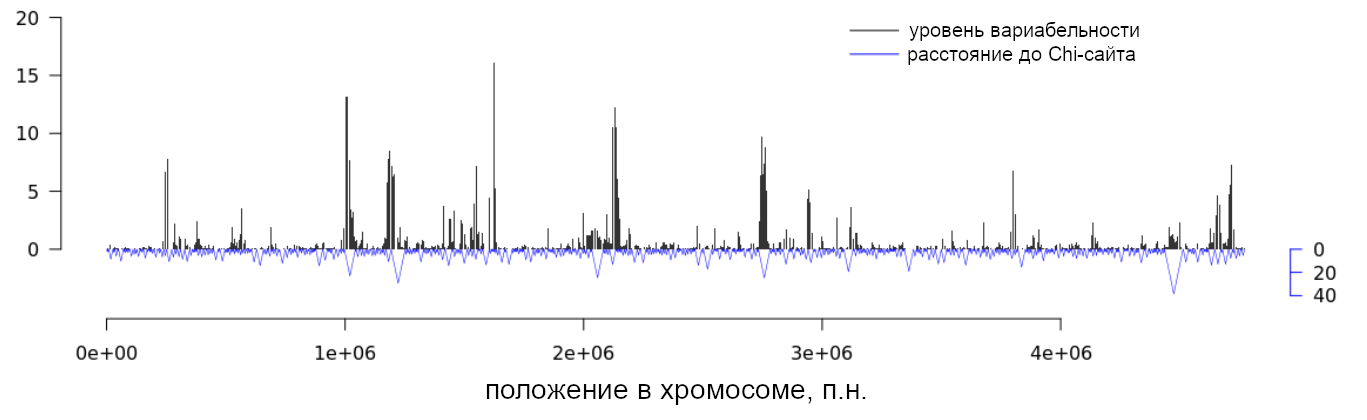
\includegraphics [width=1\textwidth] {Dissertation/images/complexity_with_smth/lf82_chi_sites.png}}
    
    \subcaptionbox{}{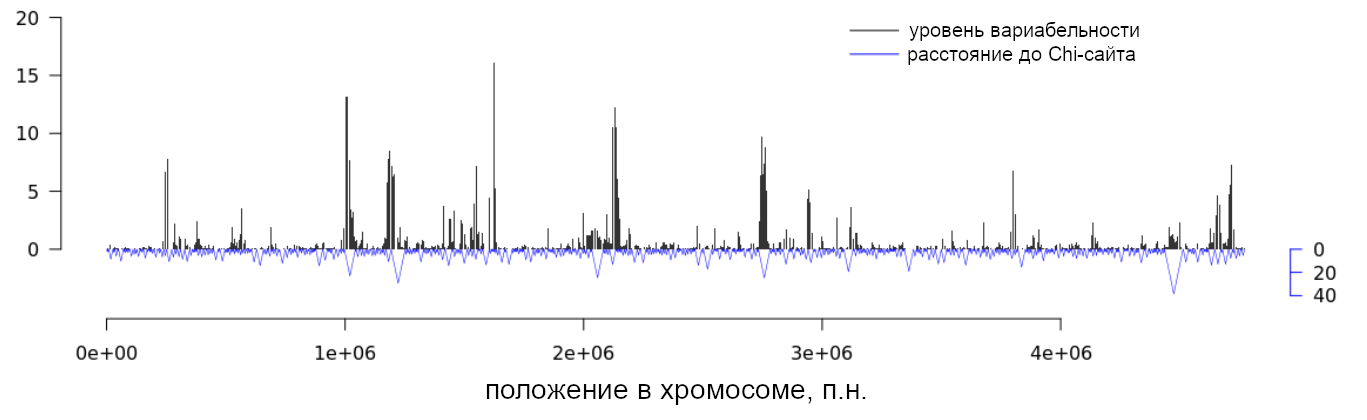
\includegraphics [width=1\textwidth] {Dissertation/images/complexity_with_smth/chidist_complexity.png}}
    
    \caption{Уровень вариабельности и локализация сайтов Chi на двух цепях хромосомы \textit{E. coli LF82}. А) Синие вертикальные линии показывают расположение сайтов Chi на двух цепях хромосомы. Вертикальные пунктирные линии показывают границы реплихор (места начала и конца репликации). Желтым и красным цветом обозначены области расположения профагов и островов патогенности соответственно. Б) Черной линией показан уровень вариабельности, синей - расстояние до ближайшего сайта Chi (в масштабе тысяч пар оснований).}
    \label{img:chi_lf82}
\end{figure}

Эффект более низкой представленности сайтов Chi в горизонтально перенесенных фрагментах был описан ранее\cite{halpern2007identification}. Вероятно, связь между вариабельностью и расстоянием до ближайшего сайта Chi объясняется тем, что вариабельные участки содержат много горизонтально перенесенных генов. 


\subsection{Связь с плотностью хромосомных контактов}


На рисунке~\ref{img:hic_matrixes} показано сопоставление профилей вариабельности с матрицами частот межхромосомных контактов для бактерий \textit{E. coli} и \textit{B. subtilis}. Очевидной связи между профилем вариабельности и частотой хромосомных контактов, с нашей точки зрения, не наблюдается.

\begin{figure}[!ht] 
  \center
    \includegraphics [width=0.9\textwidth] {Dissertation/images/complex_hic/hic_matrixes.png}
    \caption{Сравнение профилей вариабельности с нормированными матрицами хромосомных контактов для \textit{E. coli} и \textit{B. subtilis}}
    \label{img:hic_matrixes}
\end{figure}

В тоже время, признаки существования подобной связи имеются, при сравнении профиля вариабельности с шкалограммой, построенной на основе матрицы контактов (метод построения шкалограмм описан в \cite{lioy2018multiscale}), см. рисунок~\ref{img:scalogram_complexity_coli}.

\begin{figure}[!ht] 
  \center
    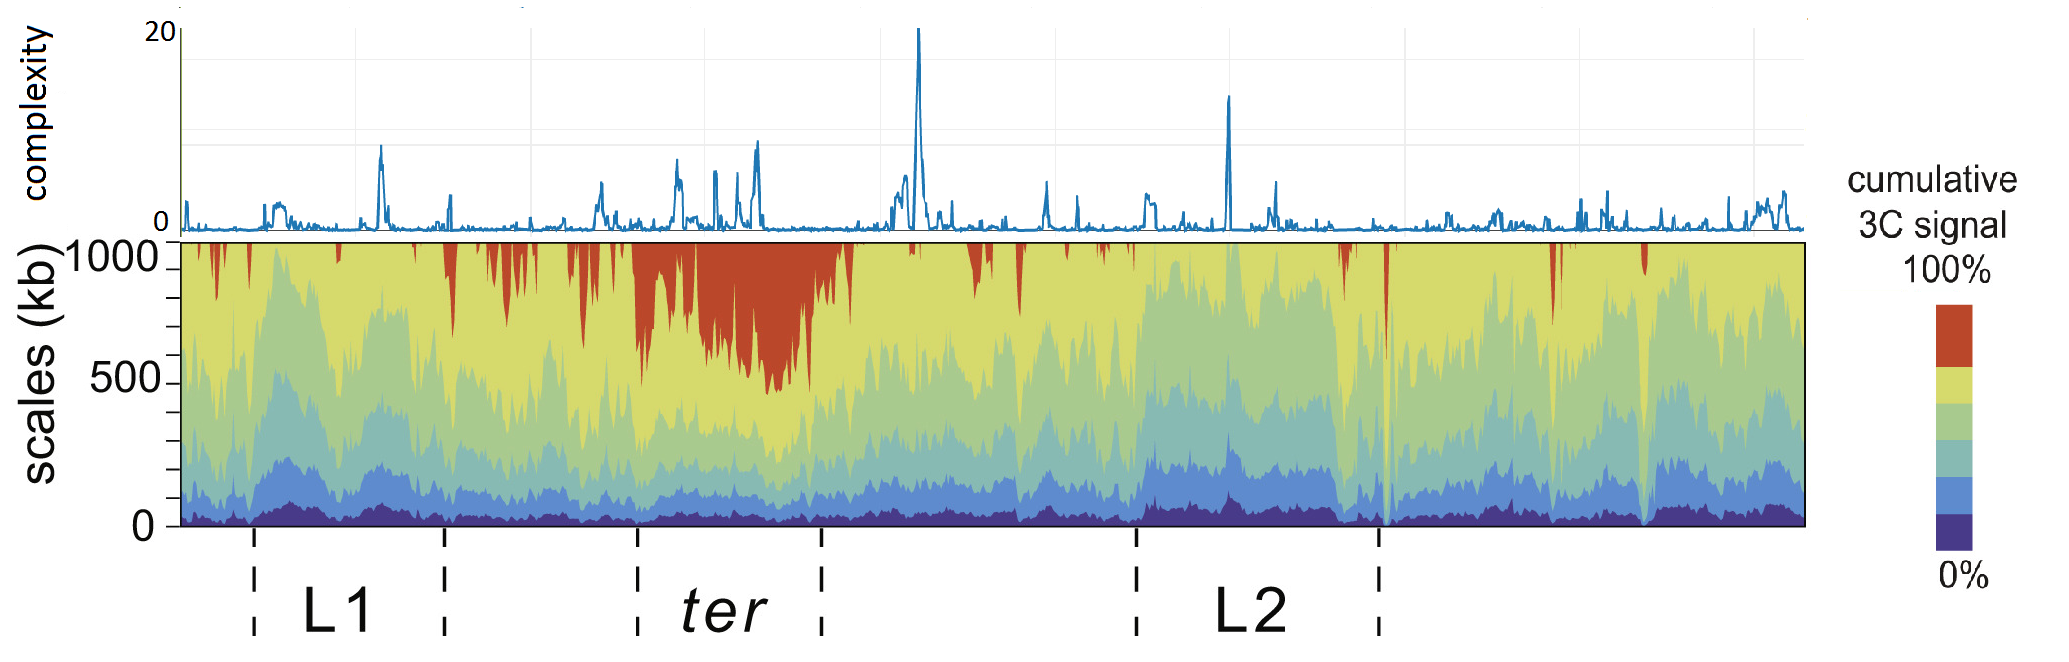
\includegraphics [width=0.9\textwidth] {Dissertation/images/complex_hic/hic_scalogram_complexity_coli.png}
    \caption{Сравнение профиля вариабельности с шкаллограммой хромосомных контактов из публикации \cite{lioy2018multiscale}.}
    \label{img:scalogram_complexity_coli}
\end{figure}

 Для оценки статистической значимости связи мы использовали линейные модели, связывающие плотность контактов в фиксированном диапазоне длин и значение вариабельности. Плотность контактов $S$ для гена с индексом $i$ считалась как сумма значений нормированной матрицы контактов $M$: $S_i = \sum_{j=1}^J M[i,i+j] $. Далее, мы строили линейные модели для связи $V_i \sim S_i$, где $V$ - это уровень изменчивости. Нами была выявлена статистически значимая зависимость между уровнем изменчивости генома и суммой межхромосомных контактов, как для бактерий \textit{E. coli}, так и \textit{B. subtilis}. 
 
 На рисунке~\ref{img:hic_coli_subtilis} приведено значение p-value для линейных моделей, связывающих значение между уровнем вариабельности генома (рассчитанным с размером окна в 20 генов) и суммой контактов, рассчитанных в окнах различного размера. В случае  \textit{E. coli} наибольшее соответствие достигается при размере окна суммирования равному 15 тысяч п.н., а в случае \textit{B. subtilis} --- 10 тысяч п.н. Это различие согласуется с различием в средней длине генов: для \textit{B. subtilis} она равна 867 нуклеотидам, а для \textit{E. coli} --- 929 нуклеотидам.

\begin{figure}[!ht] 
  \center
  \subcaptionbox{}{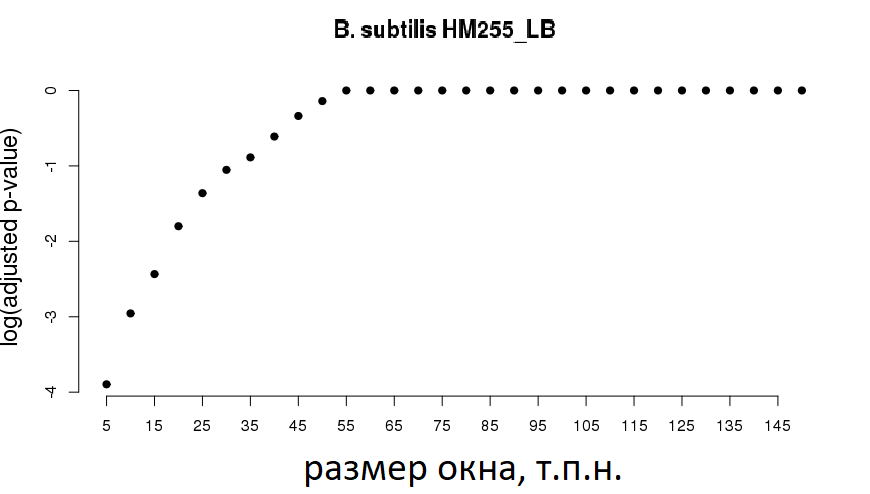
\includegraphics[width=0.6\textwidth]{Dissertation/images/complex_hic/bac_lb.png}}\hfill
  \subcaptionbox{}{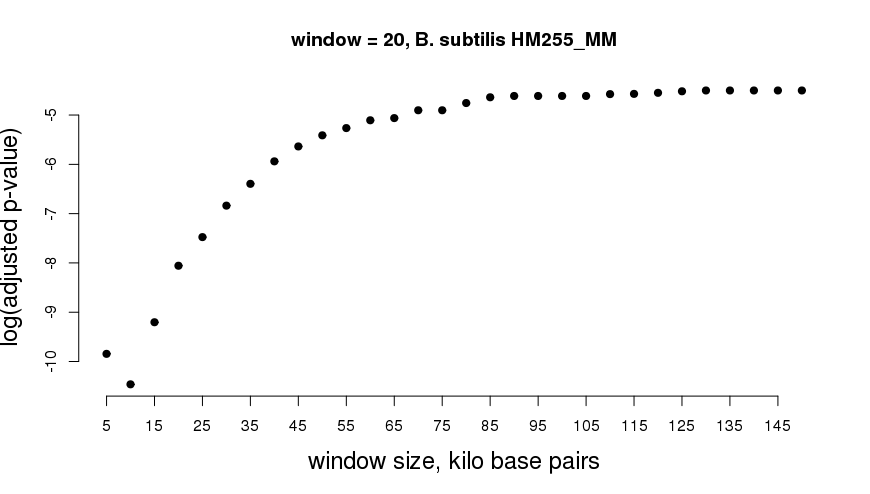
\includegraphics[width=0.6\textwidth]{Dissertation/images/complex_hic/bac_mm.png}}\hfill
  \subcaptionbox{}{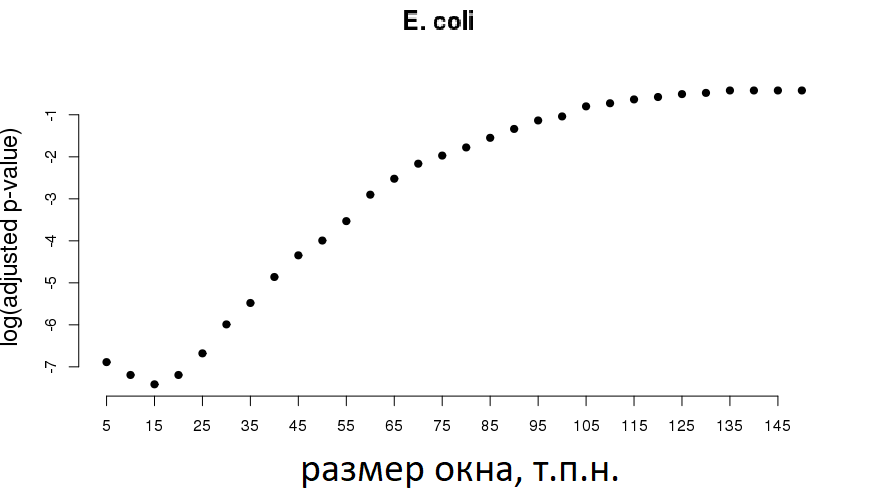
\includegraphics[width=0.6\textwidth]{Dissertation/images/complex_hic/ecoli_20.png}}

  \caption{Зависимость уровня статистической значимости (значение $p-value$) связи между уровнем изменчивости генома и плотностью хромосомных контактов. Размер окна (в тысячах пар нуклеотидов), по которому производилось суммирование значений нормированной матрицы хромосомных контактов, отложен по оси абсцисс. Десятичный логарифм значения p-value линейной модели отложен на оси ординат. На А и Б приведены значения для \textit{B. subtilis} в условиях роста на богатой среде и бедной среде, соответственно; на В приведены значения для \textit{E. coli}.} 
  \label{img:hic_coli_subtilis}  
\end{figure}

Статистическая значимость сохраняется также и при удалении главной и второстепенной диагоналей в матрице контактов (рекомендации сотрудников MIT, \url{https://www.biostars.org/p/208512/}). Так, для \textit{E. coli} значимость связи между вариабельностью и плотностью контактов в пределах 20 тысяч п.о. составляет $p-value = 1.23*10^{-7})$. Значимость ранговой корреляции при этом составила $p-value < 2.2*10^{-16}$. 
Хотя связь между уровнем вариабельности и плотностью хромосомных контактов статистически значима, она объясняет лишь малую долю вариабельности вариабельности. Так, значение $R^2$ для \textit{E. coli} составляет 0.04, а для \textit{B. subtilis} $R^2 = 0.06$.

% script is here /data4/bio/operonTravel_d4/compare_with_3c_ver2/look_with_cumuluted_contacts_v2.r





           
\section{Разработка и применение метода анализа локальной вариабельности при помощи построения подграфов}
Работа выполнена совместно с Конановым Дмитрием Николаевичем.\\


\subsection{Проблема сравнительного анализа расположения генов в большом наборе геномов.}

Визуализация блоков синтении часто применяется для сравнения генного состава оперонов, островов патогенности либо других областей генома, интересующих исследователя. Такой способ визуализации нагляден и хорошо подходит для небольшого количества геномов. Но сравнение нескольких десятков последовательностей затруднительно, а нескольких сотен --- практически невозможно. При этом, количество прочитанных геномов быстро растет, для многих видов их уже доступно несколько сотни и даже тысяч. Анализ геномов в подобных масштабах требует новых подходов. Мы предлагаем в качестве такого подхода графовое представление порядка расположения генов в геномах. Выше мы описали применение графового представления для численной оценки локальной вариабельности геномов. Ниже мы опишем применение графового представления для визуализации изменений в небольших фрагментах генома. 

\subsection{Алгоритм поиска подграфа для анализа участка генома}

Визуализация полного графа набора геномов допустима в случае небольших геномов, характерных для вирусов, но не в случае бактерий --- полный граф будет слишком велик для эффективной визуализации. Для бактериальных геномов имеет смысл проводить анализ подграфа - части полного графа, соответствующей некоторому региону интереса (например, оперону).

Для построения подграфа мы реализовали следующий набор действий. Вначале, выбирается референсный геном и указывается начало и конец анализируемой области. Затем, строится граф, содержащий цепочку узлов референсного генома и к нему добавляются узлы, представленные в других геномах и связанные с референсной цепочкой. Добавление узлов происходит пока путь снова не вернется в референсную цепочку, либо пока не будет достигнут предел на длину (параметр \textit{tails}). Алгоритм для построения подграфа можно представить следующим псевдокодом:
\begin{enumerate} 
\item Вход: graph (граф группы геномов)
\item Параметры: \textit{reference (референсный геном), start\_node (начало анализируемого фрагмента), end\_node (конец анализируемого фрагмента), max\_depth (ограничение на длину обходных путей), tails (ограничение на длину свободный путей), minimal\_edge\_weight (минимальный вес ребра)}.
\item Результат: subgraph (подграф интересующего фрагмента генома)
\item subgraph $\leftarrow$ пустой граф
\item target\_chain $\leftarrow$ цепочка узлов из референсного генома между start\_node и end\_node
\item добавить target\_chain в subgraph
\item deviating\_paths $\leftarrow$ найти все пути начинающиеся и заканчивающиеся в target\_chain
\item для каждого пути path из deviating\_paths выполнить
\item если длина path < \textit{max\_depth} то
\item  \quad  добавить path в subgraph
\item иначе
\item \quad path\_tails  $\leftarrow$ начальный и конечный фрагмент path длиной \textit{tails}
\item \quad	добавить path\_tails в subgraph
\item для каждого ребра edge из subgraph выполнить
\item \quad если вес edge < \textit{minimal\_edge\_weight} то
\item \quad \quad удалить edge из subgraph
\item удалить области связанности subgraph не связанные с target\_chain
\item вернуть subgraph
\end{enumerate}

Данный алгоритм, реализованный на языке Python3, доступен в репозитории: \url{https://github.com/DNKonanov/gene_graph_lib}

В приведенном выше алгоритме предусмотрено два фильтра, которые помогают уменьшать размер подграфа, если он оказывается слишком велик.  Даже при рассмотрении небольшого участка генома, соответствующий ему подграф может содержать длинные пути, например, из-за крупных хромосомных перестроек в рассматриваемых геномах. Для того, чтобы эти длинные пути не затрудняли визуализацию и последующий анализ, в алгоритме предусмотрен фильтр, который заменяет длинный путь его начальным и концевым фрагментом ("усами"). Максимальная длина пути, который будет показан полностью, задается параметром \textit{max\_depth}, размер фрагментов, которые сохраняются вместо длинного пути (длина "усов") задается параметром \textit{tails} (рисунок~\ref{img:tails_schema}). Пути которые начинаются либо заканчиваются, но не начинаются и заканчиваются, в рассматриваемой области ("уходящие" за пределы рассматриваемой области) также сокращаются до фрагментов длиной \textit{tails}.

\begin{figure}[!ht] 
  \center
  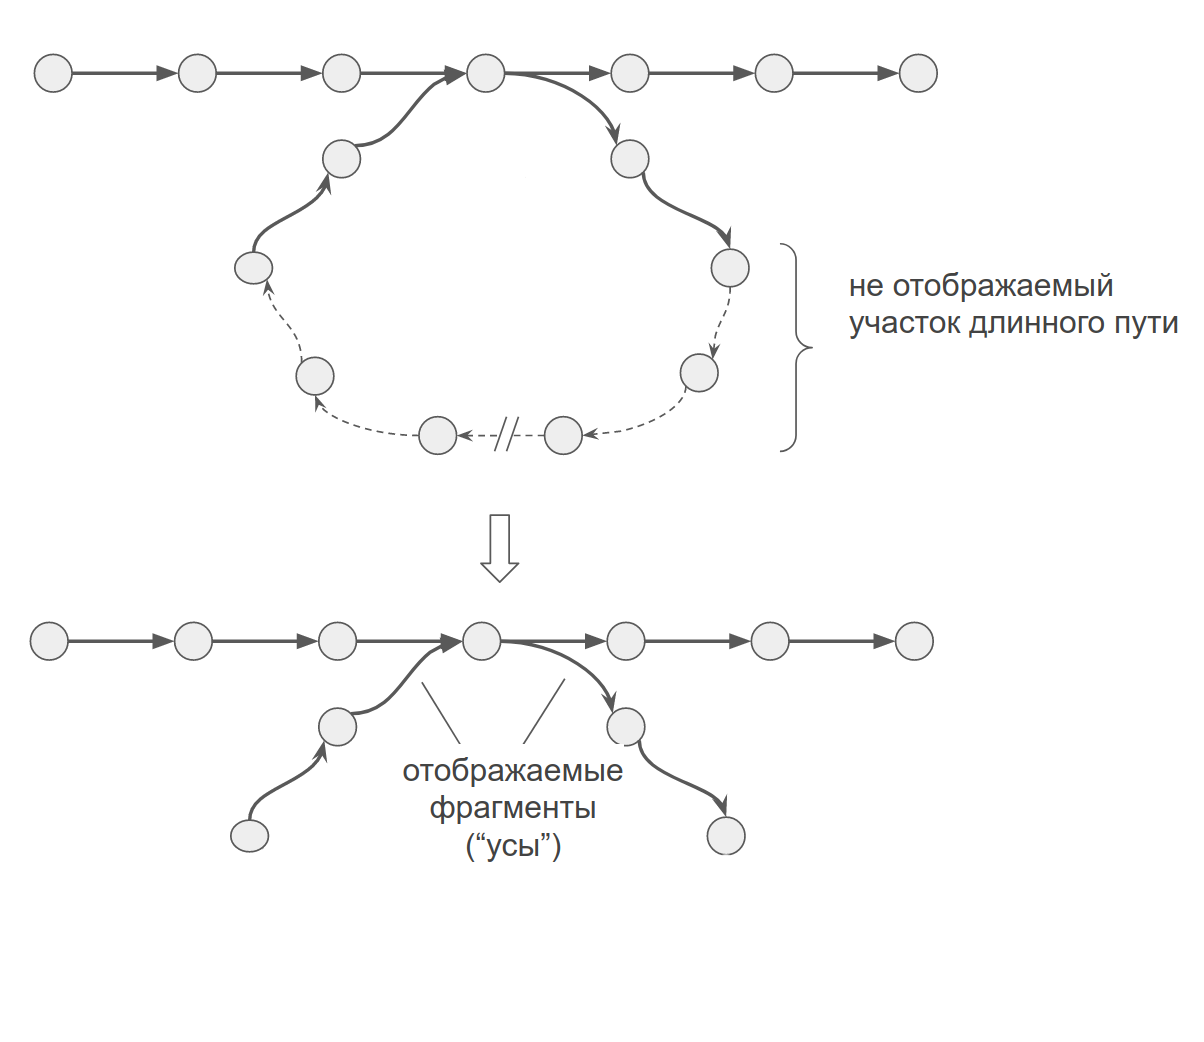
\includegraphics[width=0.8\textwidth]{Dissertation/images/subgraphs/tails_schema_v2.png}
  \caption{Схематическая иллюстрация работы фильтра длинных путей. }
  \label{img:tails_schema} 
\end{figure}

Еще один фильтр позволяет не включать в подграф ребра с маленьким весом, то есть те, которые встречаются в малом количестве геномов. За это отвечает параметр \textit{minimal\_edge\_weight}. Применение фильтров особенно важно при анализе "горячих" точек изменчивости.

%############################################################# SUBGRAPHS
\section{Примеры применения представления порядка чередования генов в виде графа.}

В работе \cite{rakitina2017genome}, были установлены опероны, которые статистически значимо чаще (метод определения будет описан ниже) встречались у изолятов \textit{E. coli} полученных от пациентов с воспалительным заболеванием кишечника --- болезнью Крона, по отношению к изолятам от здоровых людей. Носительство данных оперонов, вероятно, выгодно при нахождении бактерий в условиях воспалительной реакции со стороны организма хозяина, а может и провоцирует воспаление. Метод для поиска оперонов, различающих группы бактерий, будет описан ниже.

Рассмотрим, как выглядят подграфы, соответствующие оперонам, чья встречаемость оказалась выше в изолятах, полученных от пациентов с болезнью Крона, по сравнению с комменсальными штаммами. На этих примерах будут проиллюстрированы основные моменты анализа графового представления фрагментов генома. 

\textbf{Опероны утилизации гемина и пропандиола}

На рисунках~\ref{img:sub_hem} и ~\ref{img:sub_pdu} показаны графы, построенные в окрестностях оперонов захвата гемина (hemin uptake, hmu) и утилизации пропандиола (propanediol utilization operon, pdu), соответственно. В качестве референсного генома нами был взят геном \textit{Escherichia coli LF82}, в анализ были включены 327 финишированных геномов доступных в базе RefSeq. Для построения данных графов мы использовали следующие параметры: \textit{tails} = 1, \textit{max\_depth} = 30, \textit{minimal\_edge\_weight} = 5. 

Рассмотрим для начала более простой случай оперона захвата гемина. Данный оперона состоит из следующих генов: транспортный белок (Hemin transport protein HemS), АТФ-связывающий белок захвата гемина (Hemin import ATP-binding protein HmuV), гемин-связывающий периплазматический белок (hemin-binding periplasmic protein HmuT), кислороднезависимый копропорфириноген-III оксидазоподобный белок (oxygen-independent coproporphyrinogen-III oxidase-like protein) и два гипотетических белка (здесь и далее мы приводим аннотации последовательностей, полученные при помощи утилиты prokka \cite{seemann2014prokka}).

Как видно из графа, представленного на рисунке~\ref{img:sub_hem}, данный оперон расположен в консервативном генном контексте: слева расположен регулятор транскрипции HTH-типа, справа --- гипотетический белок. Дуговое ребро обходящее оперон сверху говорит о том, что в некотором наборе геномов данный оперон отсутствует и других вариантов генов у них в этом локусе не наблюдается. 

\begin{figure}[!ht] 
  \center
  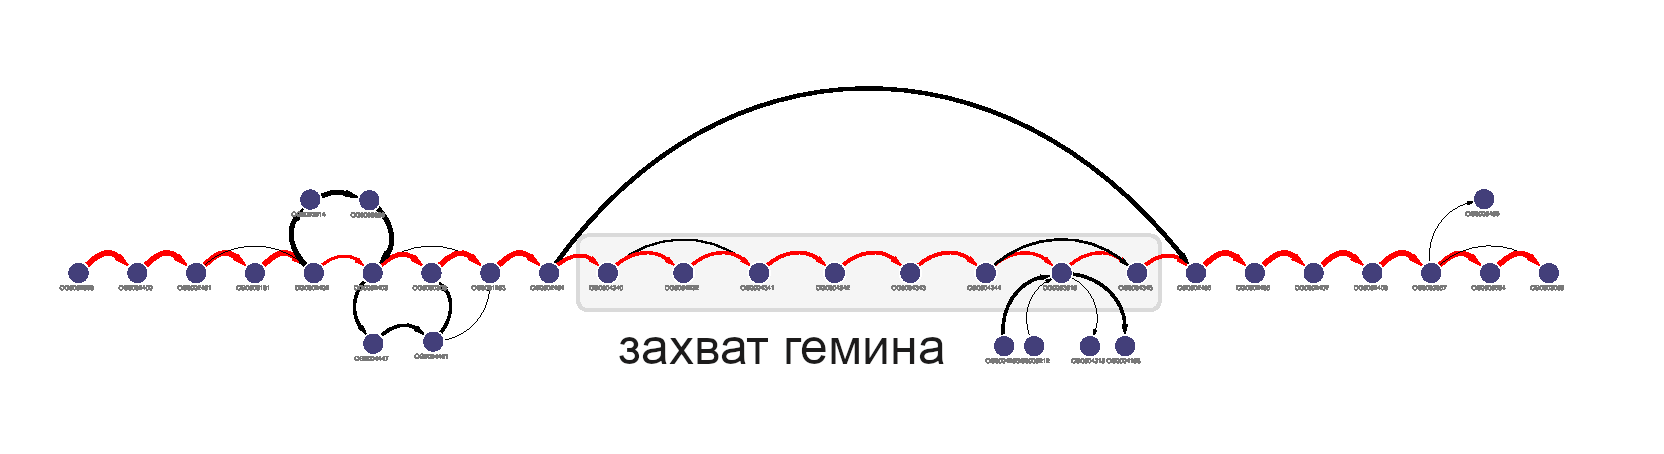
\includegraphics[width=0.8\textwidth]{Dissertation/images/subgraphs/hemin.png}
  \caption{Граф представляющий окрестность оперона утилизации гемина (hemin uptake, hmu).}
  \label{img:sub_hem} 
\end{figure}

В оперон утилизации пропандиола (propanediol utilization operon, pdu) входят гены, кодирующие: белок утилизации пропандиола PduU, малая субъединица пропандиол-дегидратазы, белок утилизации пропандиола PduB, белок с механизмом концентрации углекислого газа CcmK, субъединица альфа-фактора реактивации диолдегидратазы, белок утилизации пропандиола PduV, альдегид-алкоголь дегидрогеназа, C-диамид аденозил трансфераза ириновой кислоты Cob I, большая субъединица  пропандиол дегидратазы, фосфат-пропаноил трансфераза, альдегид-алкоголь дегидрогеназа. Как видно из рисунка~\ref{img:sub_pdu} наблюдается консервативность контекста расположения pdu оперона у тех штаммов, в которых он представлен: слева от него расположен ген, кодирующий белок CobU  (участвует в синтезе витамина B12), справа --- гипотетический белок. Ребро обходящее оперон (дуга ниже оперона) говорит о том, что в ряде штаммов в данном контексте нет иных вариантов генов. Наблюдается некоторая вариабельность внутри оперона, соответствующая нескольким вариантам данного оперона \cite{rakitina2017genome}. Помимо pdu оперона, в том же контексте, у ряда штаммов наблюдается альтернативный набор генов (узлы и ребра, расположенные выше оперона), в который входят гены транспорта железа (FepC, FcuA, HmuU), гены мобильных элементов (retroviral integrase core domain, transposase DDE Tnp ISL3) и множество гипотетических генов с неизвестной функцией. Примечательна вариабельность этого альтернативного набора генов. Вероятно, данный участок генома часто служит местом рекомбинационных событий, приводящих к изменению набора генов, причем эти изменения не имеют строгого начала и конца (т.е. не сайт специфичны), но часто накладываются друг на друга. 

\begin{figure}[!ht] 
  \center
    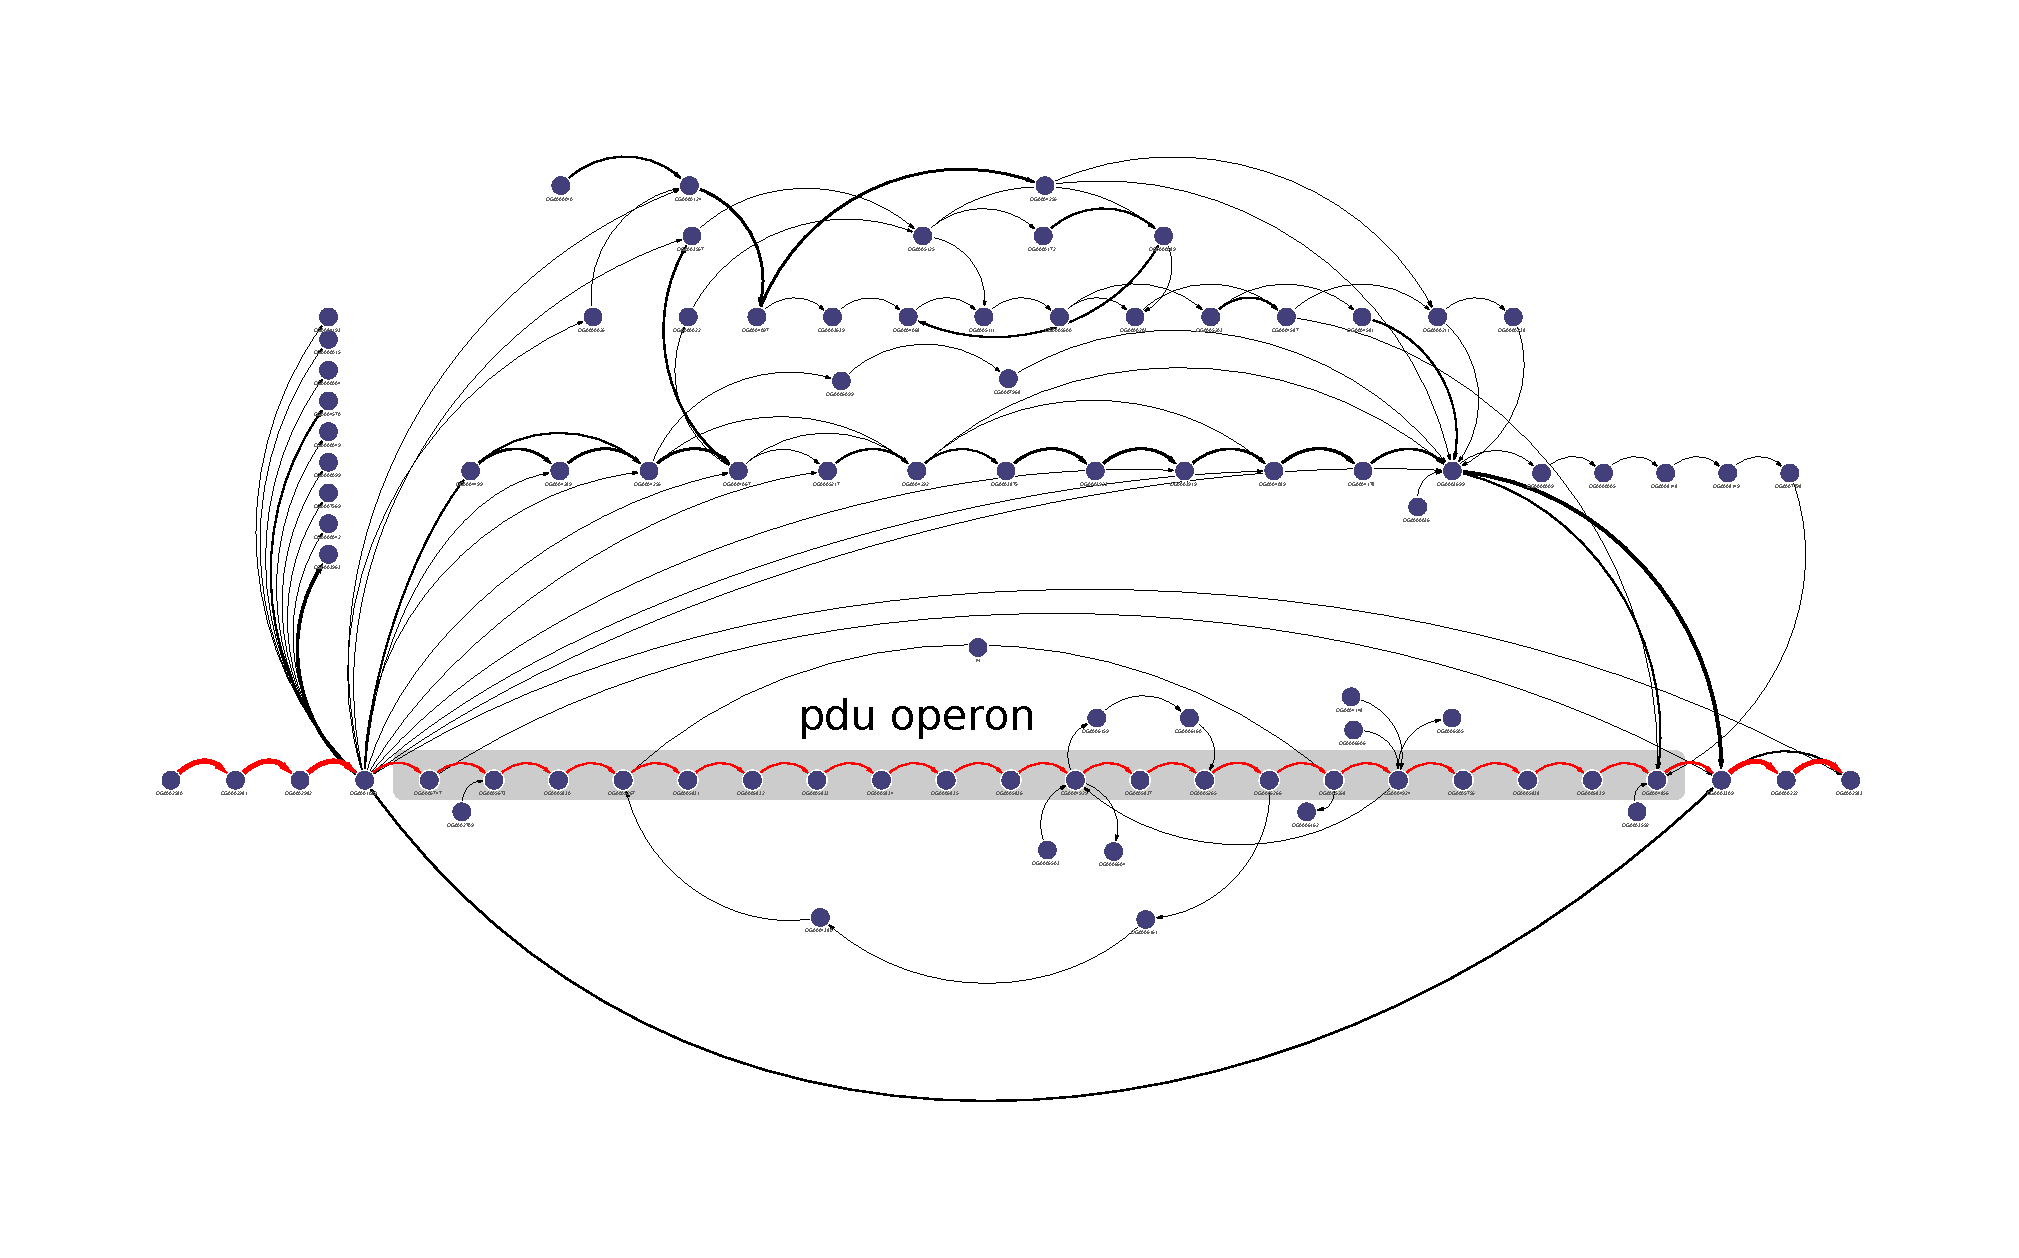
\includegraphics[width=0.8\textwidth]{Dissertation/images/subgraphs/pdutail1minw2_v2.pdf}
  \caption{Граф представляющий окрестность оперона утилизации пропандиола (propanediol utilization operon, pdu). }
  \label{img:sub_pdu} 
\end{figure}

Если рассмотреть более длинный фрагмент генома вблизи pdu оперона  (рисунок~\ref{img:pdu_wide}), видно расположенный рядом еще более вариабельный участок. Примечательно, что в нем не содержится аннотированных генов связанных с мобильностью ДНК, вместо этого присутствуют гены синтеза капсулы и многочисленные гипотетические гены с неизвестной функцией. 

\begin{figure}[!ht] 
  \center
    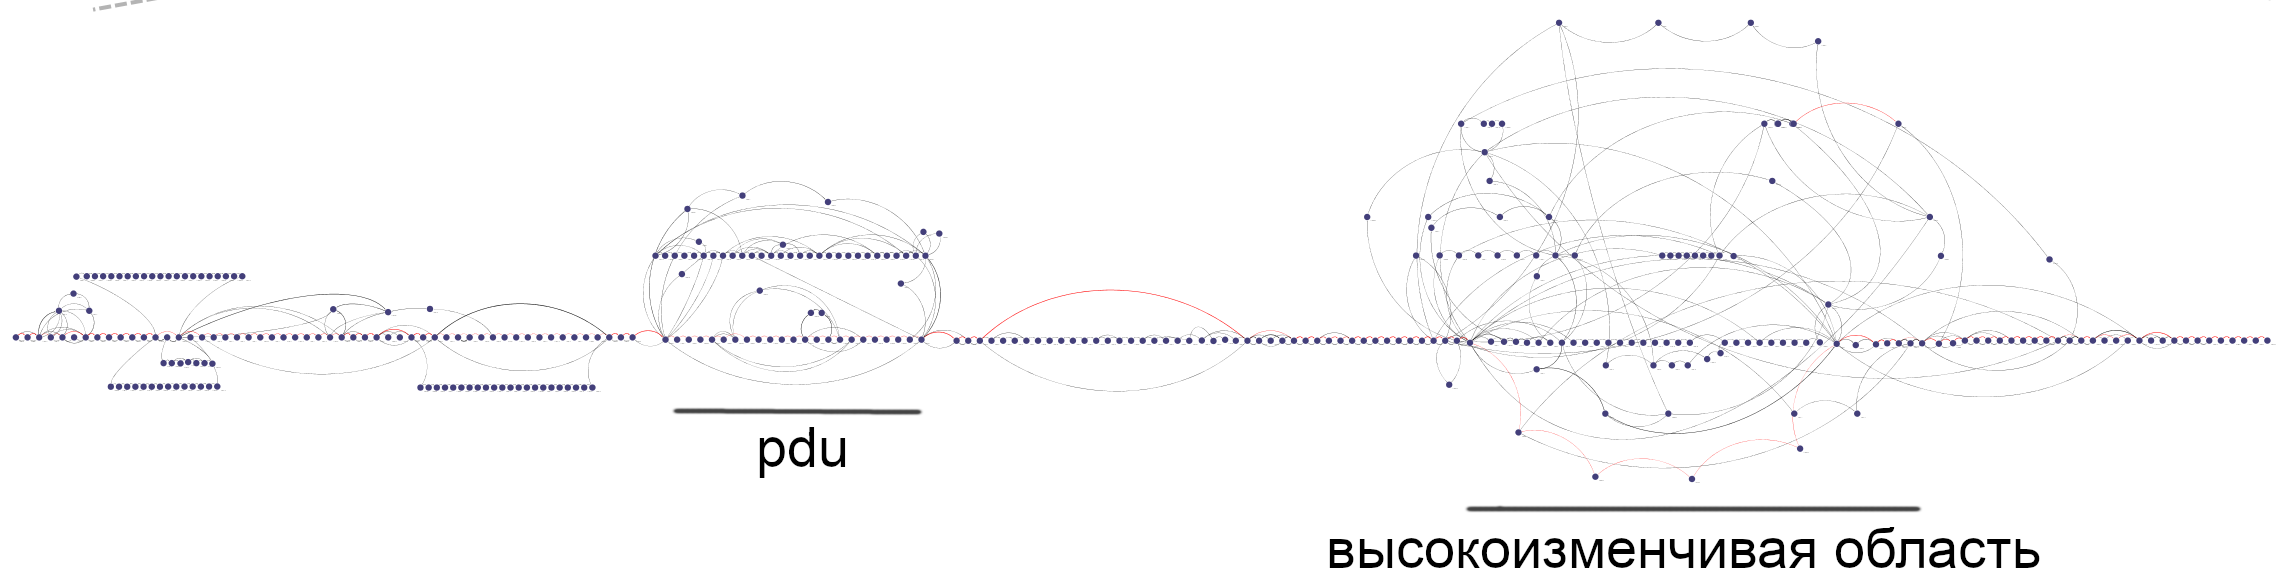
\includegraphics[width=\textwidth]{Dissertation/images/subgraphs/subgraph_largest.png}
  \caption{Граф представляющий окрестность оперона утилизации пропандиола (propanediol utilization operon, pdu). }
  \label{img:pdu_wide} 
\end{figure}

\textbf{Кластер генов синтеза бактериальной капсулы}

Перейдем к описанию графа, представляющего окружение оперона синтеза капсулы, также чаще встречающегося у изолятов из пациентов с болезнью Крона. На рисунке~\ref{img:capsule_sub_small} показано ближайшее окружение данного оперона, сам оперон обведен рамкой серого цвета. 

\begin{figure}[!ht] 
  \center
    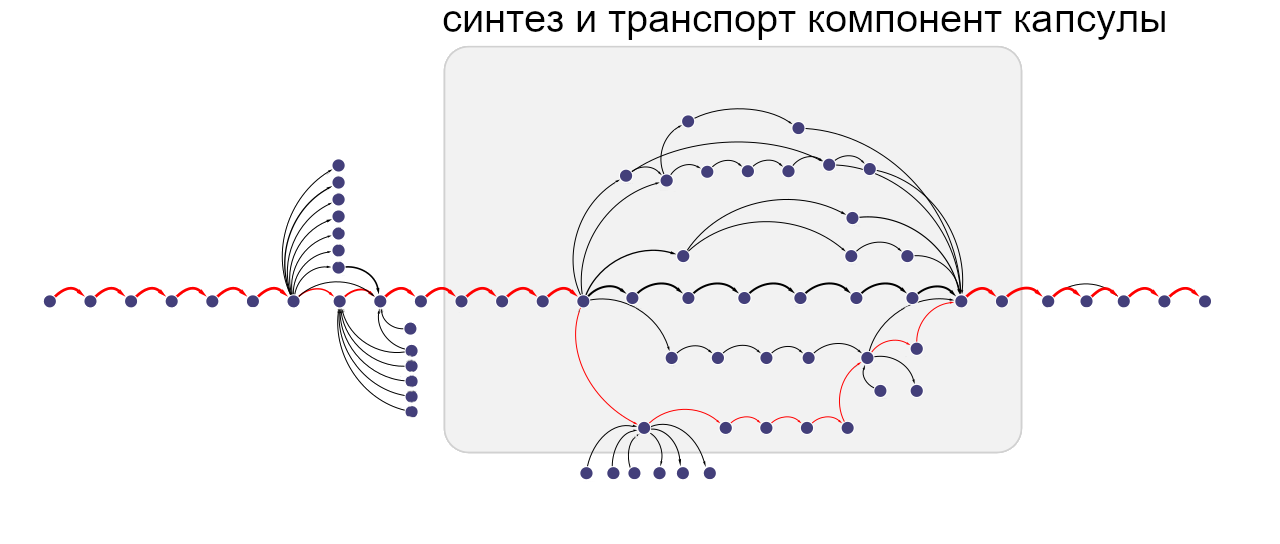
\includegraphics[width=\textwidth]{Dissertation/images/subgraphs/capsular_subgraph.png}
  \caption{Граф представляющий окрестность кластера генов синтеза бактериальной капсулы. }
  \label{img:capsule_sub_small} 
\end{figure}

Видно, что оперон состоит из консервативных фрагментов, фланкирующих вариабельный участок. Вариабельная часть оперона соответствует генам, отвечающим за синтез серотип-специфичного набора полимеров капсулы; гены консервативной части кодируют белки, участвующие в транспорте синтезированных веществ через клеточную стенку \cite{clarke1999genetic}. В референесном штамме \textit{LF82} в вариабельную часть входят гены синтеза тейхоевых кислот (teichoic acid poly ribitol-phosphate polymerase, Glycerol-3-phosphate cytidylyltransferase), в то время как мажорному варианту (путь в центре вариабельной части) соответствуют гены синтеза сиаловых кислот (polysialic acid biosynthesis protein P7, putative acetyltransferase EpsM, N,N'-diacetyllegionaminic acid synthase, N-acylneuraminate cytidylyltransferase).


Фрагменты единичной длины, расположенные на рисунке~\ref{img:capsule_sub_small} слева от оперона, говорят о том, что есть много путей, которые не попадают в построенный подграф поскольку либо слишком длинные, либо заканчиваются вне отображаемой области и поэтому были сокращены до коротких фрагментов (параметр \textit{tails} при анализе был равен 1). Если расширить рассматриваемую область, то многие из этих путей станут видны (рисунок~\ref{img:capsule_sub_large}, данный граф получен с параметрами: \textit{tails} = 1, \textit{minimal\_edge} = 2). Вид данного графа говорит о значительной вариабельности участка генома, содержащего гены синтеза капсулы.

\begin{figure}[!ht] 
  \center
    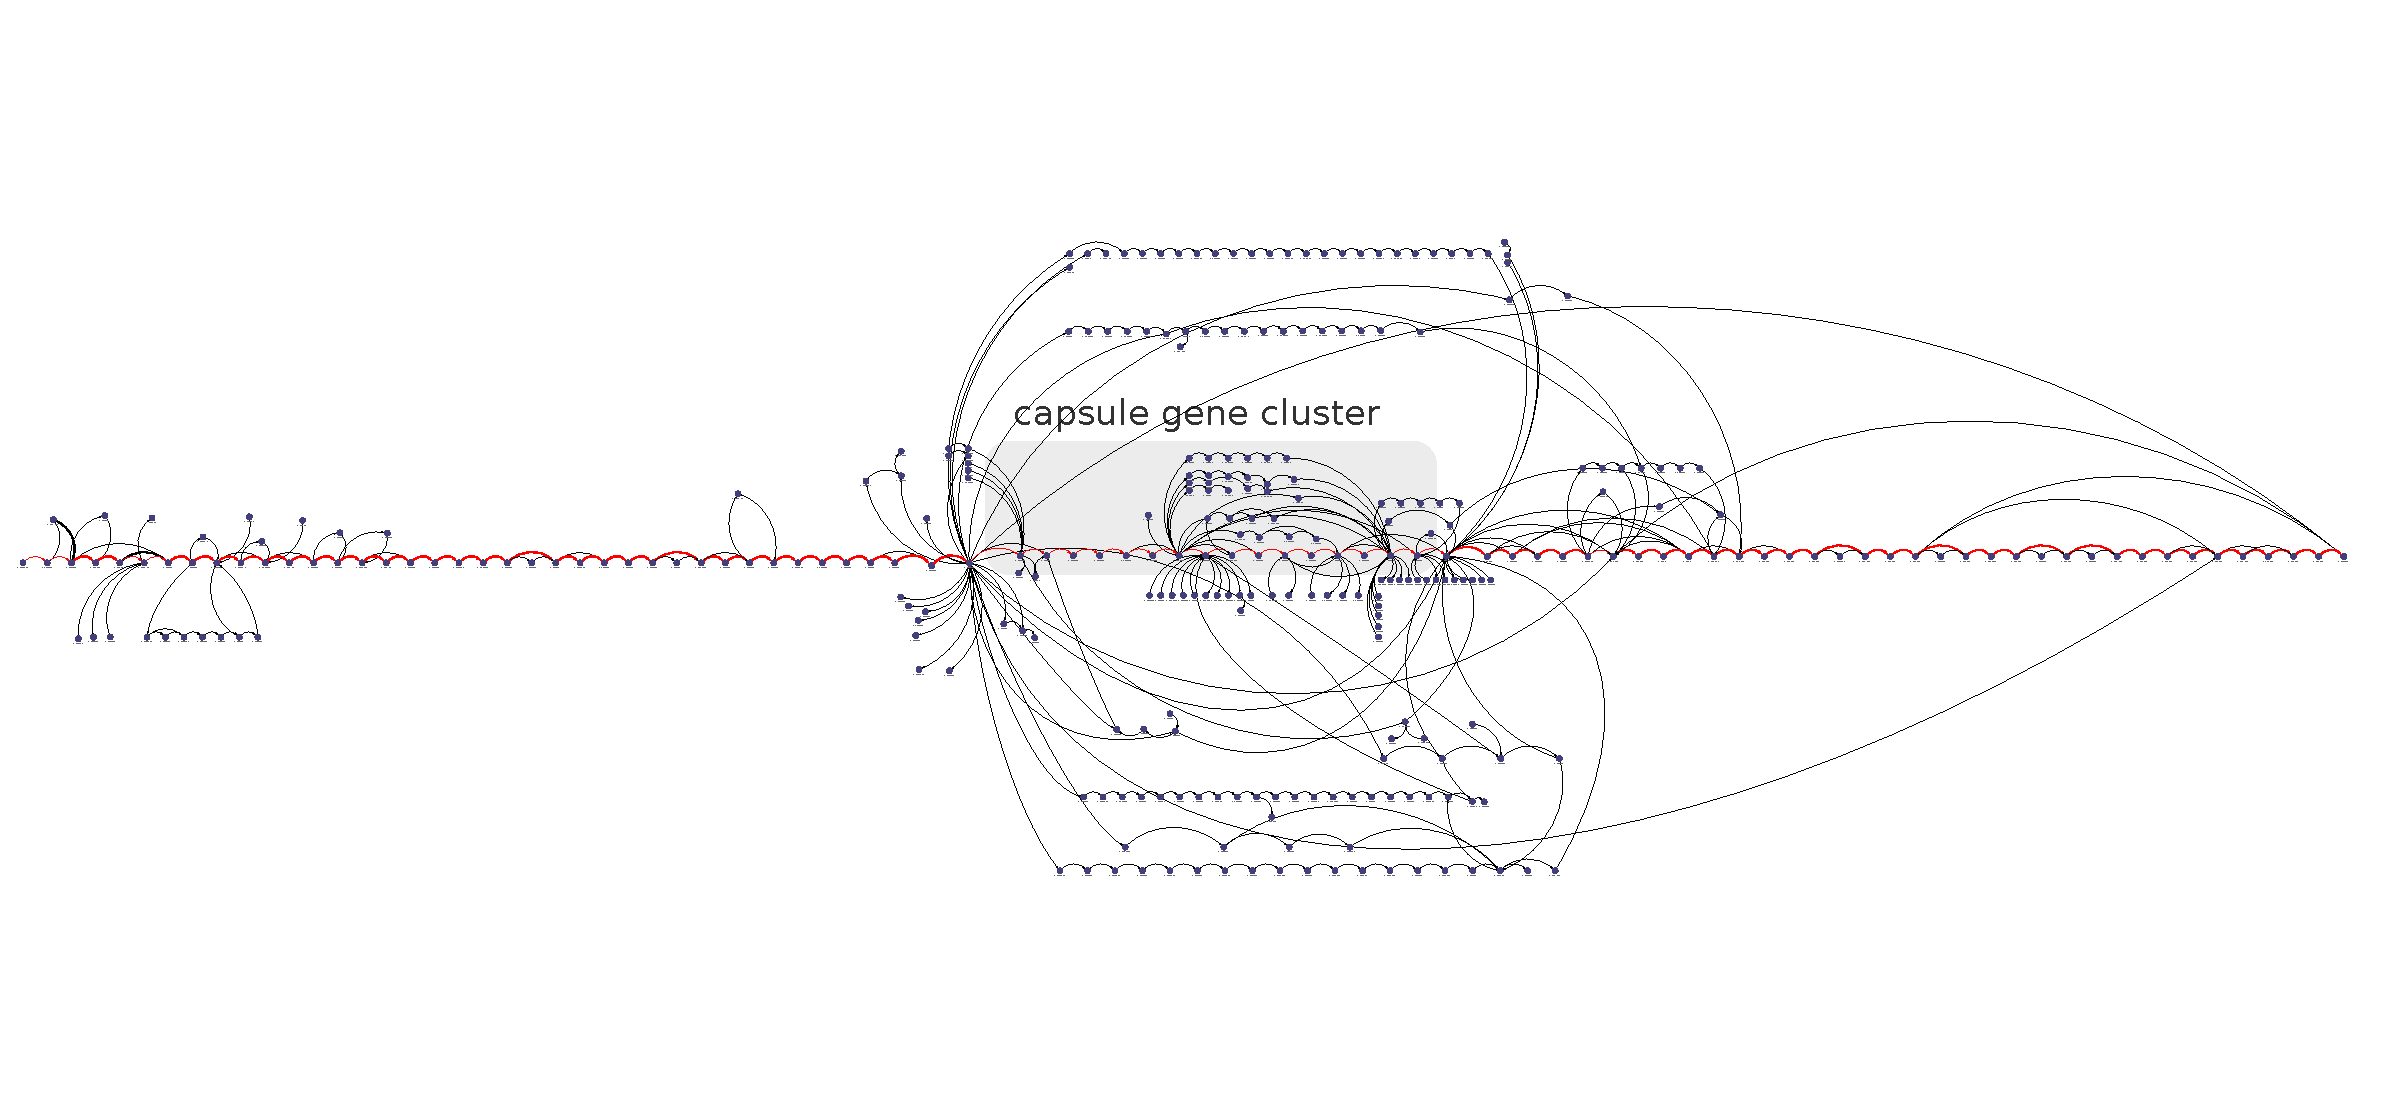
\includegraphics[width=\textwidth]{Dissertation/images/subgraphs/capsular_subgraph.pdf}
  \caption{Граф представляющий расширенную окрестность генов синтеза бактериальной капсулы. }
  \label{img:capsule_sub_large} 
\end{figure}

Вариабельность состава капсулы адаптивна (это помогает бактериям избегать распознавание иммунной системой организма-хозяина либо бактериофагами \cite{cress2014masquerading, lukavcova2008role}. Можно предположить, что для бактерии выгодно такая локализация этих генов, где изменения могут происходить чаще. Можно выдвинуть гипотезу, что данный участок генома обладает некоторыми (еще не установленными) свойствами, которые обеспечивают значительную вариабельность генного состава, и в том числе - вариабельность состава генов капсулы.

\textbf{Оперон метаболизма глиоксилата}

На рисунке~\ref{img:glioxilate} показан граф отражающий область генома в окрестности оперона метаболизма глиоксилата. Данный оперон является частью геномного острова, содержащего ген ibeA, продукт которого связывается с рецепторами эндотелиальных клеток головного мозга. Данный остров описан у вызывающего менингит штамма \textit{Escherichia coli K1}, и, методом экспериментального мутагенеза, показан как функционально значимый для проявления ее патогенных свойств \cite{huang2001novel}. Остров содержит четыре оперона: ассоциированный с инвазией оперон ibe, а также три оперона метаболизма углеводородов и глицерола (ptn, cgl, gcx) \cite{rakitina2017genome}. 

\begin{figure}[!ht] 
  \center
    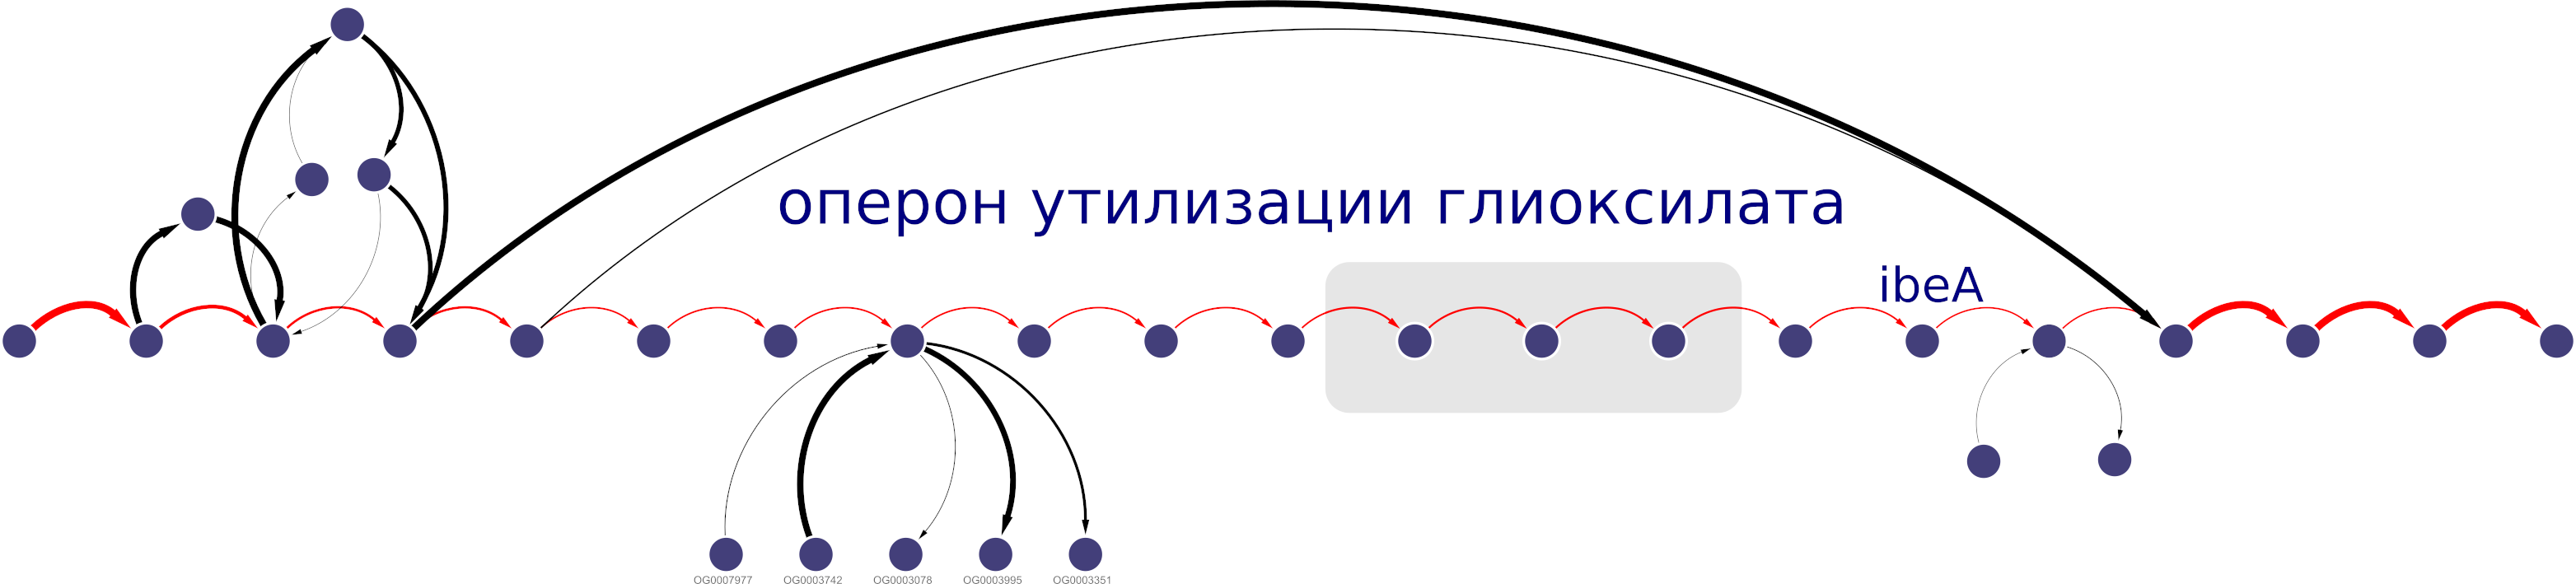
\includegraphics[width=\textwidth]{Dissertation/images/subgraphs/glyoxilate_metabolism_operon_crop.png}
  \caption{Граф представляющий окрестность генов оперона метаболизма глиоксилата. }
  \label{img:glioxilate} 
\end{figure}

% Замечание: мелко! продумать рисунки

Интересно, что хотя мы наблюдали значительную вариабельность геномных островов у \textit{E. coli} и других бактериальных видов, в данном случае наблюдается весьма низкая вариабельность генного состава: остров либо представлен у некоторых организмов, либо - нет, и в последнем случае, на его месте не обнаруживаются какие-либо вставки.

\textbf{Оперон захвата и утилизации сорбозы}

В случае данного оперона наблюдается картина схожая с опероном захвата химина и глиоксилата: оперон либо присутствует у части штаммов, либо нет, без выраженной изменчивости генома в данном регионе (рис.~\ref{img:sorbitol}). 

\begin{figure}[!ht] 
	\center
	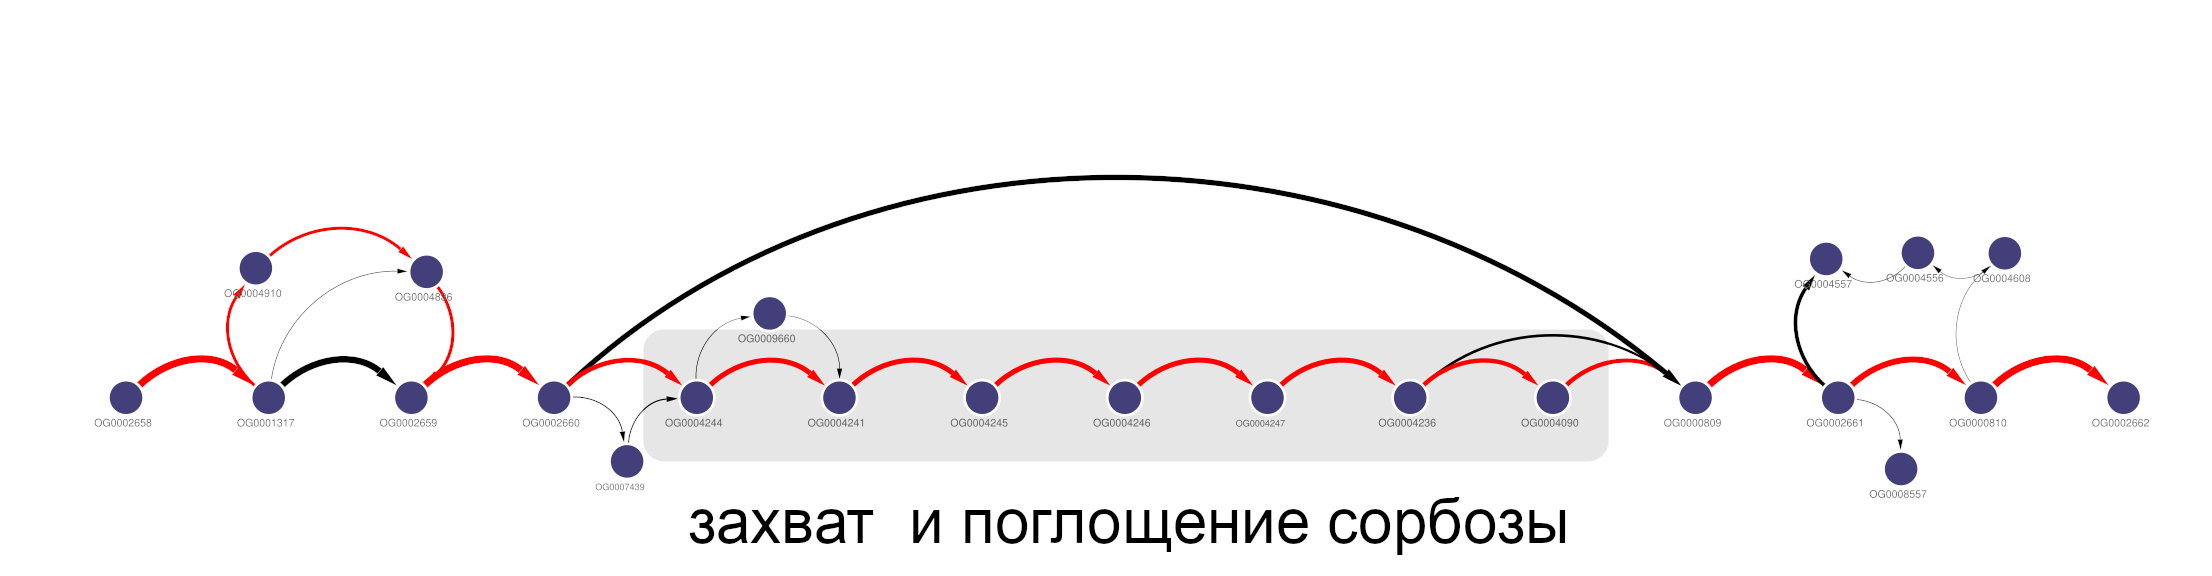
\includegraphics[width=\textwidth]{Dissertation/images/subgraphs/sorbitol.png}
	\caption{Граф представляющий окрестность генов оперона захвата и утилизации сорбозы. }
	\label{img:sorbitol} 
\end{figure}

%Добавить: последний граф для профага и обобщение
           
\section{Разработка компьютерного приложения для анализа вариабельности геномов} \label{chaptGCB}

Выполнено совместно с Конановым Дмитрием Николаевичем.

Оценка профиля изменчивости вдоль хромосомы и построение подграфов для фрагментов геномов - варианты анализа геномной изменчивости. Они 
позволяют проводить анализ на уровне отдельных репликонов (напрмер, хромосомы) в первом случае, и на уровне небольших геномных локусов (например, оперонов) - во втором. Для проведения анализа на двух уровнях одновременно мы разработали приложение Genome Complexity Browser (GCB). Данное приложение доступно на веб-сервере по адресу \url{gcb.rcpcm.org}, и может быть звпущенго на локальном компьютере пользователя. Веб-версия содержит пред просчитанные данные для 143 видов. Использование локальной версии необходимо для анализа групп геномов не представленных на веб-сервере. Интерфейс программы показан на рисунке~\ref{img:gcb_face} и состоит из трех основных частей: области визуализации профиля изменчивости, области визуализации подграфов для выбранных областей генома и боковой панели с настройками и элементами управления (поиск генов, экспорт/импорт файлов).
 
\begin{figure}[!ht] 
	\center
	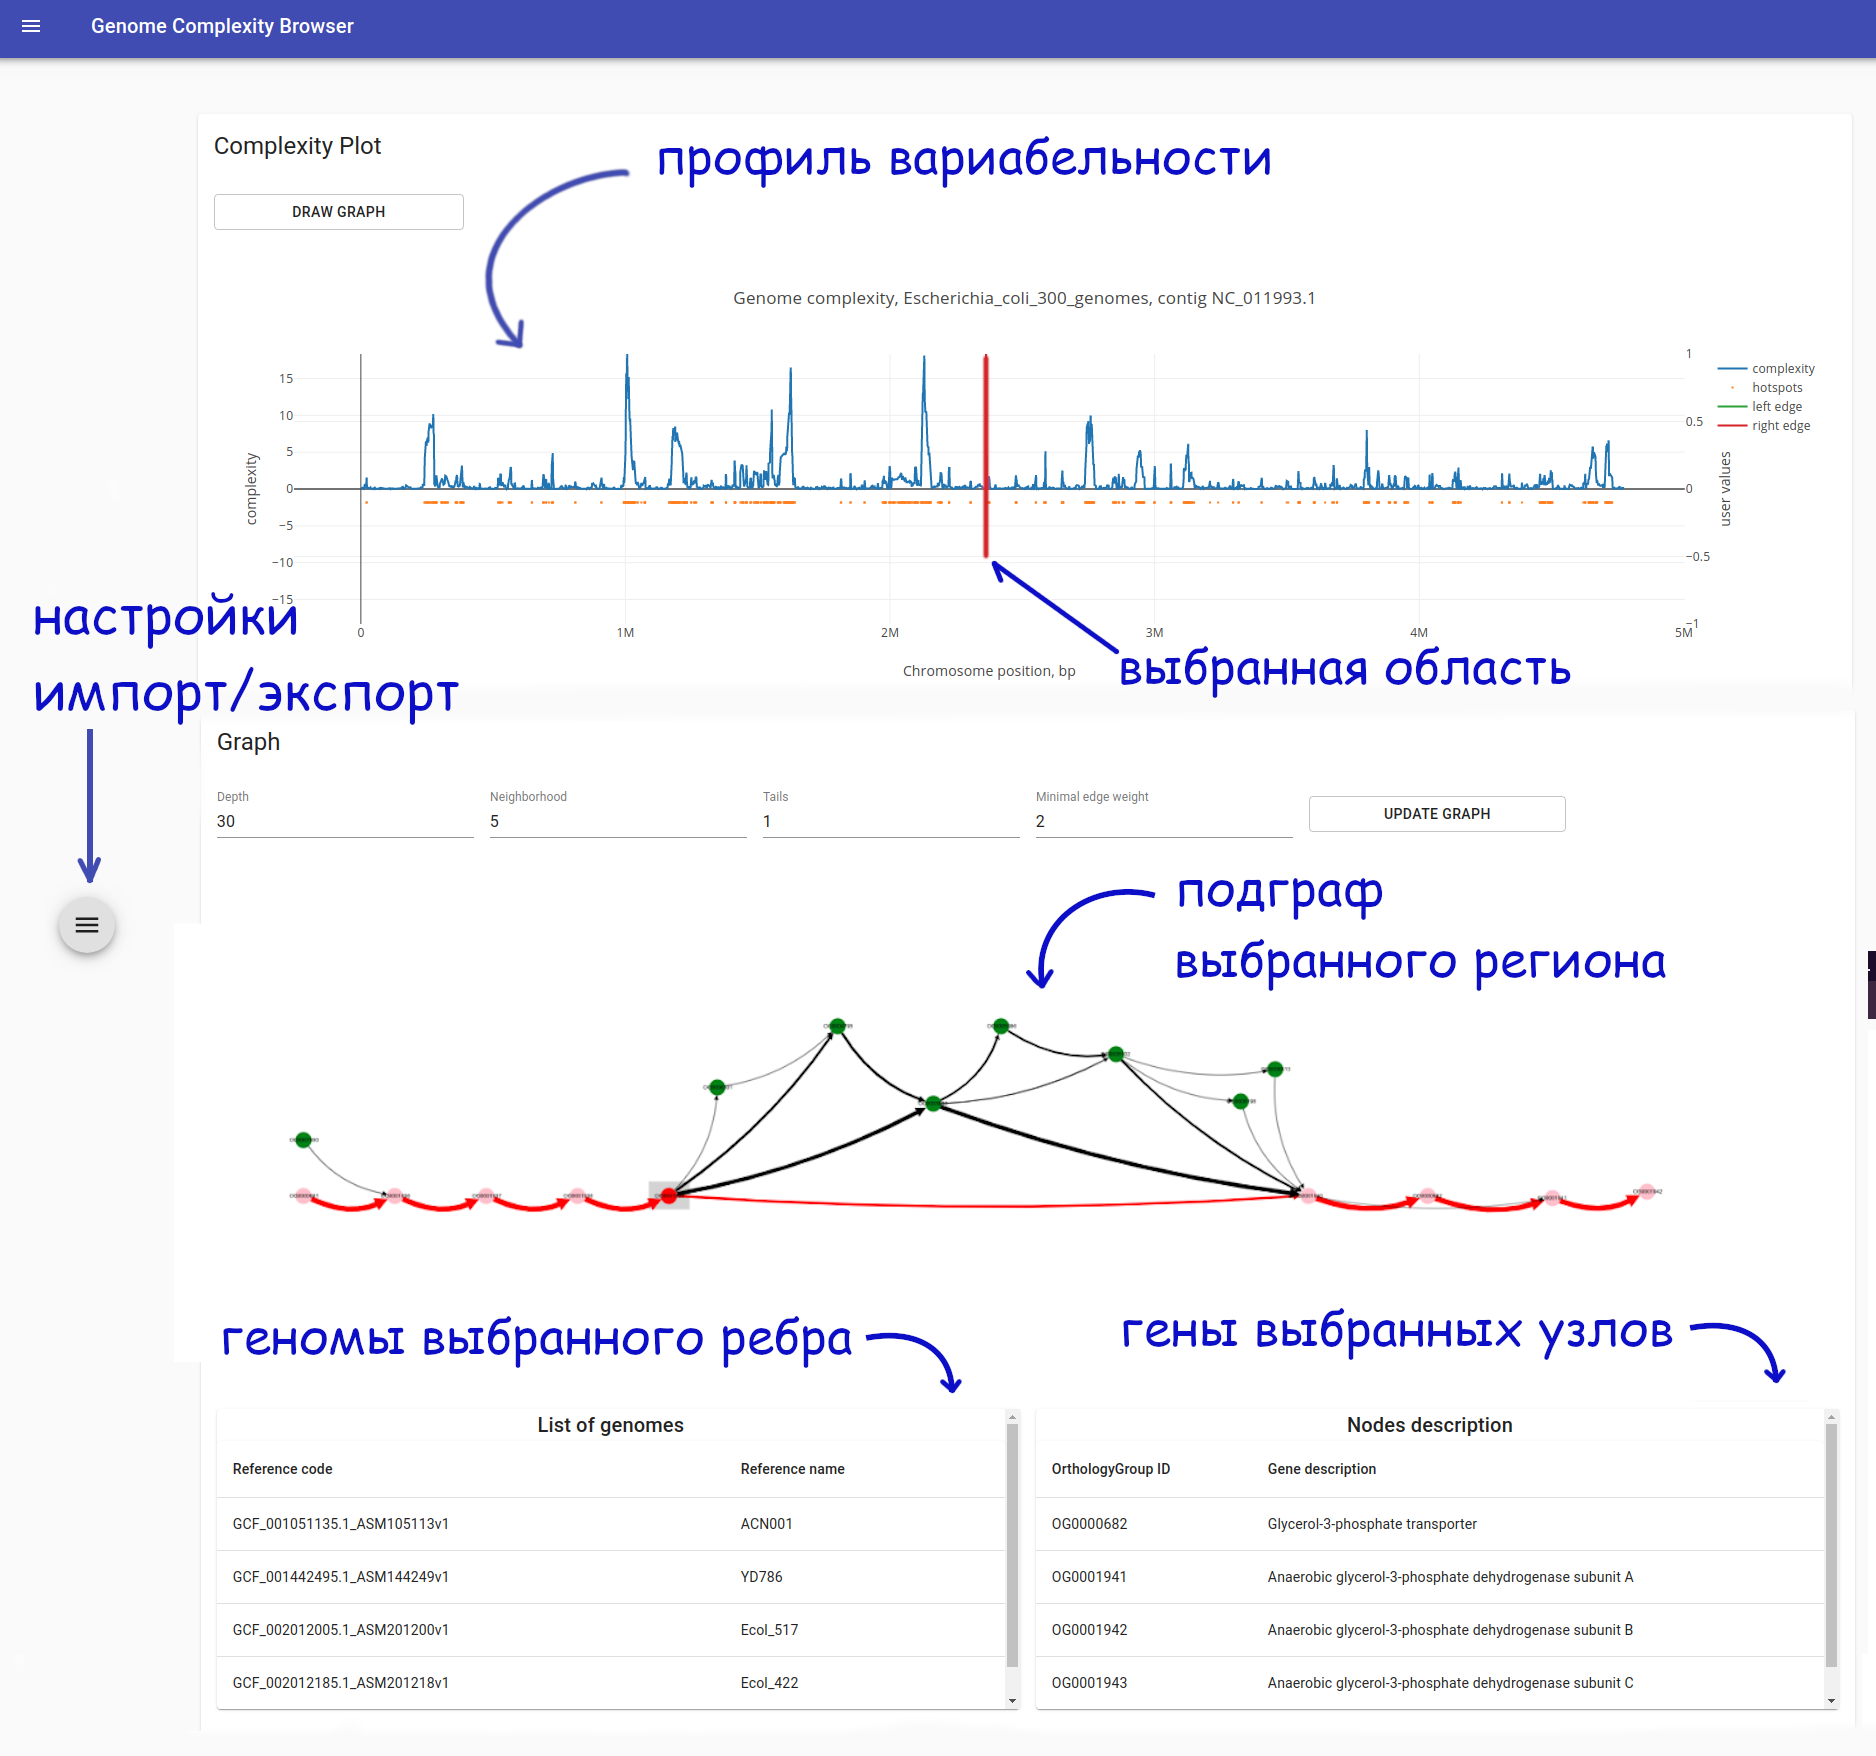
\includegraphics [width=0.9\textwidth] {Dissertation/images/gcb/gcb_face_text.png}
	\caption{Графический интерфейс программы Genome Complexity Browser.}
	\label{img:gcb_face}
\end{figure}

Основные сценарии использования программы следующие:

I. Интерес представляет некоторый оперон или группа генов.

Пользователь выбирает организм, геном и задает координаты области интереса. Происходит построение подграфа для выбранной области. При необходимости, пользователь меняет параметры визуализации (например, увеличивает минимальный отображаемый вес ребра для исключения редко встречающихся комбинаций генов, в случае если получаемый граф слишком сложен для анализа). Экспорт полученной визуализации в графическом формате, либо в формате XML для последующей визуализации подграфа в программе Cytoscape (графовый редактор). 

II. Интерес представляют области повышенной либо пониженной изменчивости генома.

Пользователь выбирает организм и геном. Происходит визуализация профиля изменчивости выбранного генома. Пользователь может выбрать интересующий его регион генома (например, область с максимальным уровнем изменчивости) и выполнить визуализацию подграфа в данной области - таким образом можно установить, какие гены содержатся в данном локусе у различных геномов, и каков паттерн зафиксированных в ходе эволюции изменений. Пользователь может экспортировать профиль изменчивости в виде текстового файла, для последующей визуализации (например, сравнение профилей изменчивости разных организмов), либо сохранить области с повышенной изменчивостью в файл в формате BED. 

\textbf{Возможности программы}

В программе предусмотрено автоматическое выделение "горячих точек" изменчивости. Они отображаются на профиле изменчивости (точки оранжевого цвета, расположенные ниже профиля), и их положение можно скачать в виде файла в формате BED. Для выделения областей повышенной изменчивости, мы использовали критерий Тьюки: искали значения уровня вариабельности, которые превышают 75 перцентиль на полтора межквартильных расстояния \cite{tukey1977exploratory}. 

Для анализа геномов, недоступных на веб-сервере \url{gcb.rcpcm.org}, необходимо использование локальной версии программы. Вначале подготовить (расположить в одной папке) интересующие пользователя геномы, затем запустить конвеер orthoSnake (доступен по адресу: \url{https://github.com/paraslonic/orthosnake}) и консольное приложение gg.py (доступно по адресу \url{https://github.com/DNKonanov/geneGraph}) - в итоге, будет создан файл с базой данных, содержащей графовое представление геномов и значения изменчивости. Файл с базой данных необходимо скопировать в папку, куда была установлена локальная версия сервера GCB, после этого можно работать с интерфейсом программы в веб-браузере. Схема анализа показана на рисунке~\ref{img:gcb_scheme}, полный пример (с установкой всех зависимостей и проведением анализа) доступен по адресу: \url{https://gcb.readthedocs.io/en/latest/standalone.html#complete-step-by-step-example}.

\begin{figure}[!ht] 
	\center
	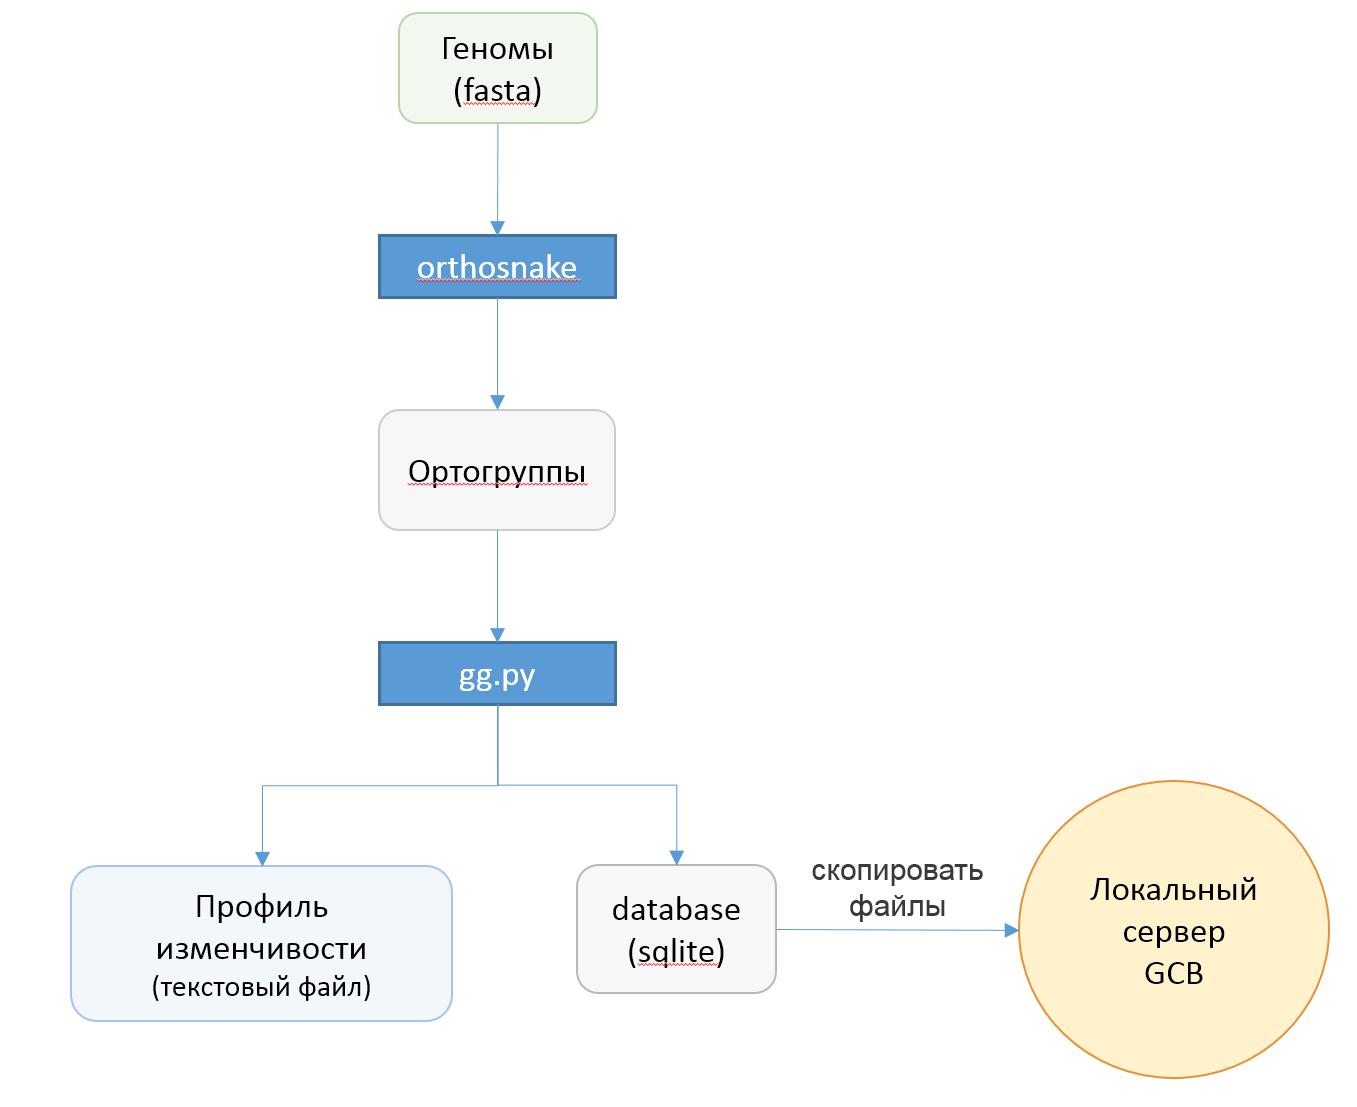
\includegraphics [width=0.9\textwidth] {Dissertation/images/gcb/standalone_scheme.png}
	\caption{Графический интерфейс программы Genome Complexity Browser.}
	\label{img:gcb_scheme}
\end{figure}

Документация и видеоматериалы по использованию программы (как веб-версии, так и консольных утилит) доступны по адресу \url{gcb.readthedocs.io}. 
  
% https://github.com/paraslonic/bacgenome_assembly <- may be add description of this

\section{Алгоритмизация подхода выявления оперонов, наличие которых ассоциировано с определенным признаком. } \label{chaptOperons}

\subsection{Проблема поиска генетических ассоциаций для субпопуляций бактерий}
Предположим, что у нас есть некоторый признак, по которому мы можем разбить набор геномов на группы, и наша задача - установить, какие гены значимо чаще (либо реже) встречаются в одной из групп. Распространенным подходом в подобном случае является оценка значимости по каждому отдельному гену. После проведения этих тестов необходимо применить поправку на множественное сравнение, так как иначе следует ожидать множество ложно положительных результатов. В случае, если работа ведется на данных о полной последовательности генома, имеется большое количество анализируемых генов (порядка $10^3 - 10^4$), а размеры групп, как правило, незначительны (порядка $10^1 - 10^2$), что приводит к тому, что после поправки на множественное сравнение, ни один из анализируемых генов не проходит даже низкие пороги на значимость. В качестве одного из способов преодоления описанной выше проблемы мы предложили использовать информацию об организации генов в опероны для поиска значимых ассоциаций \cite{rakitina2017genome}. Рассматривая оперон как структурную единицу, мы значительно сокращаем количество анализируемых признаков, так, что оно становится сравнимым с размерами групп.

\subsection{Алгоритм поиска генетических ассоциаций}
Первым шагом выполняется оценка значимости в точном тесте Фишера по каждому гену независимо. Затем ищутся опероны, в которых количество генов с заданным уровнем значимости выше, чем ожидается при случайном распределении генов по оперонам. Для оценки количества, ожидаемого при случайном распределении, применяется метод случайных перестановок либо оценка, основанная на распределении Пуассона. В первом случае, перестановки производятся в таблице соответствий генов и оперонов и подсчитывается максимальная доля значимых генов в оперонах данной длины. Во втором случае, на основе наблюдаемого количества генов с уровнем значимости превышающим пороговый, раcсчитывается их средняя плотность на единицу длины и затем для каждого оперона оценивается вероятность наблюдать данное либо большее количество подобных генов в соответствие с распределением Пуассона. И в первом, и во втором случае, финальным шагом является проведение поправки на множественное сравнение, но уже не для генов, а для оперонов, количество которых, как правило, значительно ниже общего количества генов.

Алгоритм первого подхода можно записать следующим образом:\\
Пусть $I$ - набор оперонов, определенный на референсном геноме $R$.
\begin{enumerate} 
  \item Определить группы ортологии $O$.
  \item Для каждой группы ортологии $o \in O $ имеющей хоть один ген, представленный в $R$, посчитать $P\textsubscript{o} = $p-value в точном тесте Фишера.
  \item Для каждого оперона $i \in I$ посчитать $Fobs\textsubscript{i} = $доля входящих в него генов, для которых $P\textsubscript{o} < 0.05$.
  \item Для каждого $j \in [1..10000]$
  	\begin{enumerate} 
        \item Провести случайную пермутацию значений $P$ .
        \item Для каждого оперона $i \in I$ посчитать $Frnd\textsubscript{i, j} = $доля генов, для которых $P\textsubscript{o} < 0.05$.
  	\end{enumerate} 
  \item Для каждого оперона $i \in I$ найти $Fmaxrnd\textsubscript{i}=max\textsubscript{j}(Frnd\textsubscript{i, j})$ - максимальную долю генов в опероне при случайных перестановках значений значимостей для генов.
  \item Для каждого оперона $i \in I$, если $Fobs\textsubscript{i}>Fmaxrnd\textsubscript{i}$, считать его значимым с уровнем значимости $p{}$.
\end{enumerate}

Перейдем к описанию результатов применения данного подхода.

\subsubsection{Поиск оперонов, значимо чаще встречающихся у изолятов бактерий \textit{E. coli}, изолированных от людей с болезнью Крона.}
В анализе был использован 51 геном \textit{E. coli}, из которых 27 были геномы бактерий, изолированных от больных с болезнью Крона, а 24 генома принадлежали изолятам, полученным от здоровых людей. При помощи программы OrthoFinder \cite{emms2015orthofinder} мы получили 11885 ортогрупп. Далее, при помощи точного теста Фишера, для каждой ортогруппы мы оценили статистическую значимость ее неравномерной представленности в группах. Минимальное значение p-value, при этом, было меньше, чем 0.00037, а медианное - 0.78. После поправки на множественные сравнения (метод Бенджамини-Хохберга \cite{benjamini1995controlling}) минимальное значение p\-value составляет 1 (такой же результат дают методы Бенджамини-Йекутили \cite{benjamini2001control} и Холма \cite{holm1979simple})). Код для проведения данного анализа доступен в репозитории \url{https://github.com/paraslonic/Rakitina_etal_Crohn_paper/blob/master/ogEnrichment/calcFDR.r}. 

Следующим шагом мы осуществили описанный выше тип анализа, для поиска значимо дифференциально представленных оперонов. Информация об оперонах была взята из базы данных DOORS \cite{mao2014door}. В качестве референсного генома мы использовали геном \textit{Escherichia coli LF82} - данный штамм был изолирован из пациента с болезнью Крона и является модельным в исследованиях адгезивно-инвазивного фенотипа у кишечной палочки \cite{miquel2010complete}. Затем, мы провели 10000 случайных перестановок соответствий между генами и оперонами. Для каждой перестановки мы вычисляли зависимость количества генов в оперонах с p-value < 0.05 от длины оперона. Визуализация сравнения наблюдаемых и полученных при случайных перестановках результатов показана на рисунке~\ref{img:operons_shuffle}. Опероны, для которых наблюдаемое число генов было выше, чем максимальное количество генов при случайных перестановках, считались статистически значимо пере- либо недо-представленными, поскольку для них можно считать, что в пермутационном тесте p-value < 0.0001. 

\begin{figure}[!ht] 
  \center
    \includegraphics [width=0.75\textwidth] {Dissertation/images/operons/statsignificant_operons.pdf}
    \caption{Зависимость доли генов в оперонах, с уровнем значимости p-value < 0.05, от количества генов входящих в оперон. Пунктирная линия показывает максимальные значения, полученные при проведении 10000 случайных соотнесений генов и оперонов. Синим цветом выделены точки, соответствующие оперонам, которые неравномерно представлены между группами согласно пермутационному тесту.}
    \label{img:operons_shuffle}
\end{figure}

Так, например, оперон утилизации пропандиола состоит из 19 генов, из которых 14 генов (74\%) имеют p-value < 0.05 в точном тесте Фишера. При проведении 10000 случайных пермутаций уровней значимости по генам, в данном опероне в среднем наблюдалось 3\% генов, а максимальная доля составила 21\%. Таким образом, можно сделать вывод, что повышенная представленность данного оперона в изолятах из пациентов, но не здоровых людей, не является случайным наблюдением. Полный список оперонов, определенных как значимо чаще встречающихся у изолятов из пациентов с болезнью Крона приведен в таблице~\ref{tbl:ops1}. 

\begin{table}[htbp]
  \centering
  \caption{Список оперонов статистически значимо пере-представленных в группе штаммов \textit{E. coli} изолированных от пациентов с болезнью Крона. N - количество генов, Pobs - наблюдаемая доля перепредставленных генов в опероне, Pmean - средняя доля перепредставленных генов при случайных пермутациях, Pmax - максимальная доля перепредставленных генов при случайных пермутациях.}
  \label{tbl:ops1}
  \setlength{\fboxsep}{10pt}%
  \setlength{\fboxrule}{0pt}%
  \fbox{
  \begin{tabular}{|l|l|l|l|l|}
  \hline
  \textbf{N} & \textbf{Pobs} & \textbf{Pmean} & \textbf{Pmax} & \textbf{функция}                                  \\ \hline
  4          & 1             & 0.03          & 0.75         & утилизации глиоксилата \\ \hline
  6          & 0.83          & 0.02          & 0.67         & синтез и экспорт капсулы      \\ \hline
  6          & 1             & 0.02          & 0.67         & захват гемина                                       \\ \hline
  7          & 0.86          & 0.03          & 0.57         & утилизации сорбозы                             \\ \hline
  19         & 0.74          & 0.03          & 0.21         & утилизации пропандиола                         \\ \hline
  \end{tabular}
  }
  \end{table}

Исходный код программ, определяющих опероны, статистически значимо чаще встречающихся у изолятов, полученных от пациентов с болезнью Крона, доступен в репозитории \url{https://github.com/paraslonic/Rakitina_etal_Crohn_paper/blob/master/operonPval/}.

\graphicspath{{Dissertation/images/}}

\chapter{Обсуждение. } \label{chaptDiscussion}


В настоящее время, для некоторых видов прокариот доступны сотни и даже тысячи геномов. Постоянно пополняющуюся коллекцию геномных последовательностей можно использовать для получения информации о вариабельности генома, его архитектуре, устройства различных оперонов, геномных островов и иных мобильных элементов.

Инструменты визуализации синтении (например, Mauve, BRIG, genePlotR) часто используются для сравнительных исследований геномов прокариот и вирусов. Они позволяют визуально определить наличие больших и малых перестроек генома, но применимы для сравнительно небольших количеств сравниваемых геномов (10-20), а при большем размере выборки визуальный анализ становится затруднителен. В настоящее время существует недостаток методов визуализации сравнения большого (превышающих десятки) количества геномов и численной оценки изменчивости геномов. Подобного рода инструменты необходимы для исследования структуры генома, отдельных геномных элементов и изучения факторов, влияющих на возникновении либо исчезновение высокоизменчивых областей генома и областей с пониженной изменчивостью.

Для эффективного анализа и визуализаций больших наборов геномов мы предложили подход на основе графов, в котором гены представлены в виде узлов, узлы связываются между собой ребром, если соответствующие гены расположены последовательно в одном из геномов. Такое представление позволяет создавать компактные визуализации изменчивости определенного локуса в десятках и сотнях геномов. Мы также предложили использовать подсчет путей на графе для оценки изменчивости геномных последовательностей. 

Графы имеют давнюю историю применения в анализе геномов. Они давно применяются для сборки геномов из множества коротких прочтений. При этом узлами графа служат либо сами прочтения, либо отдельные подстроки фиксированной длины (k-меры). Поиск оптимального обхода на графе дает оптимальное выравнивание прочтений (либо k-меров), что позволяет воссоздать последовательность генома. Применяются также методы картирования прочтений на набор референсных геномов, представленных в виде графа. Такой подход позволяет учесть уже известные варианты геномов для более полного картирования прочтений. 

Графы применялись также для анализа изменчивости генома. В нескольких работах группы Е. Кунина использовалось графовое представление расположения кластеров ортологичных групп (COG) во множестве геномов. Значительное распространение получило представление перестроек генома в виде графов разрыва (brakepoints graph), удобное для реконструкции предковых состояний генома, но не для задач визуализации. 

В нашей работе, мы использовали представление набора геномов в виде графа для двух задач: численной оценки уровня изменчивости в отдельных локусах генома и визуализации подграфов, соответствующих отдельным областям генома. Визуализация подграфов позволяет дать ответы на ряд вопросов о контексте генов интереса. Например, находится ли ген или гены интереса в одинаковом окружении во всех рассматриваемых геномах? Какие альтернативные генные контексты существуют и в каких геномах они представлены? Какие части набора генов (например, оперона или генного острова) являются консервативными, а какие вариабельными? Какие геномы содержат определенную комбинацию генов? 

Мы провели поиск оперонов, которые чаще встречаются у кишечных палочек, выделенных из образцов фекалий и кишечных смывов пациентов с болезнью Крона - тяжелого воспалительного заболевания кишечника. Функция большинства найденных оперонов ясна, они позволяют микробу захватывать железо, утилизировать пропандиол (продукт переработки слизистого слоя), менять антигенные свойства, тем самым убегая от иммунного ответа. Интересно, что анализ графов, представляющих контекст этих генов, показал очень разные картины. Два оперона: утилизации пропандиола и производства капсулы находятся в высокоизменчивых -- "горячих"\ -- областях генома. Опероны утилизации гимина, утилизации глиоксилата, захвата сорбозы напротив находятся в "тихих"\ областях. Роль генетических факторов, находящихся в областях генома с разным уровнем изменчивости, в формировании генотипа и фенотипа бактерий --- предмет дальнейших исследований. В случае оперона синтеза и экспорта капсульных полисахаридов, можно предположить, что нахождение данного оперона в "горячей"\ области генома может способствовать более высокой изменчивости состава оперона (у него есть высоко вариативная часть, отвечающая за синтез капсулы), что в свою очередь выгодно для эффективного избегания иммунного ответа организма-хозяина.

При помощи графового представления геномов мы реализовали метод количественной оценки локальной изменчивости, основанный на поиске уникальных путей в подграфе. Под изменчивостью в данном случае мы понимаем изменение состава либо взаимного расположения генов в геноме. Под локальностью --- то, что изменения затрагивают небольшую область генома, не превышающую размер выбранного окна анализа (выбирается пользователем, обычно, составляет около 20-40 генов). Насколько нам известно, разработанный нами вычислительный конвейер (Genome Complexity Browser, GCB) является первым доступным инструментом, который позволяет количественно определять изменчивость генома на основе заданного пользователем набора геномов. GCB предоставляет способ оценки профиля изменчивости вдоль репликонов, что позволяет находить "горячие точки"\ генома, в которых уровень изменчивости значительно выше, чем в остальной части генома, и его "тихие"\ области. 

Нам представляется перспективным направление исследований, включающее поиск изменений в интенсивности и местоположении "горячих"\ и "тихих"\ областей. Такой анализ можно проводить при помощи сравнения профилей изменчивости на разных уровнях филогенетического сходства: между геномами из различных внутривидовых структур (например, клад филогенетического дерева или экотипов) или между геномами близких видов. Результатом подобных исследований должно стать знание факторов, влияющих на уровень изменчивости генома в отдельных его областях. GCB позволяет оценивать изменчивость в определенном локусе генома (на основании задаваемых пользователем близкородственных геномов). Размер локуса может задаваться параметром окна, указываемом при запуске программы. Анализ геномов при помощи скользящего окна позволяет получить профиль уровня изменчивости вдоль генома. Мы предусмотрели метод автоматического определения областей повышенной изменчивости на основе критерия Тьюки (критерий учитывает медианное значение и межквартильный размах).

Для проверки применимости предложенного метода мы провели вычислительные эксперименты по моделированию эволюции бактериальных геномов. Мы допустили возможность вставки, удаления, перемещения генов, а также геномные инверсии. Вероятность этих событий была не равномерна вдоль модельной хромосомы, но менялась в соответствии с задаваемым профилем. Таким образом, в основе моделирования лежало предположение, что в геноме существуют области повышенной и пониженной изменчивости, положение которых устойчиво во времени. Затем мы оценивали профиль изменчивости на основе полученных геномов и предложенного нами подхода. Мы наблюдали высокий уровень сходства исходных и вычисленных профилей. Вероятность геномных инверсий в наших экспериментах была на два порядка ниже, чем остальные события, что согласуется с наблюдаемой частотой у многих бактериальных видов. Этот параметр крайне важен для применимости метода: для эффективной оценки локальной изменчивости, глобальные перестройки генома не должны нарушать понятие локальности. 

В применимости нашего подхода нас также убеждает анализ областей генома, содержащих известные "горячие точки"\ изменчивости: интегроны и геномные острова. Данные области обладают высоким уровнем изменчивости при анализе предложенным методом, резко выделяясь на фоне прилегающей части генома. 

Профиль изменчивости генома \textit{E. coli} обладает ярко выраженной контрастностью. На нем видны протяженные участки с низкой изменчивостью и области, в которых изменчивость очень высока. Большинство областей с высокой изменчивостью совпадает с локализацией профагов, либо описанных ранее островов патогенности. Существуют также "горячие"\ точки, включая и наиболее изменчивые области, внутри которых нам не удалось обнаружить следов мобильных элементов (такое же наблюдение описано в исследовании \cite{oliveira2017chromosomal}). Протяженность низко-изменчивых областей оказалась выше (наиболее протяженная область составляет порядка миллиона пар нуклеотидов), высокоизменчивые области как правило короче (наиболее длинные области достигают длины в 200-300 т.п.н.).

Мы сравнили профили изменчивости геномов \textit{E. coli} из пяти основных филогрупп: A, B1, B2, D и E. Для каждой филогруппы был выбран один референсный геном и сто ближайших к нему геномов из базы RefSeq, для каждого набора из 101 геномы мы провели анализ изменчивости независимо. Референсные геномы обладали достаточно высоким уровнем сохранности структуры генома (без крупных перестроек), что позволило сравнивать расположение областей повышенной и пониженной изменчивости. Сравнение показало, что множество областей повышенной изменчивости расположено в близких по контексту областях генома. Значительная часть этих областей соответствует профаговым областям, так что их консервативное расположение можно объяснить сайт-специфичным характером их встраивания и изменчивостью самих фаговых геномов. Особенно заметна роль профагов в вариабельности геномов из филогруппы E (референсный геном: \textit{O157:H7 Sakai}). Интересно, что области интеграции разных фагов значительно различаются по уровню своей изменчивости. Ряд областей повышенной изменчивости геномов, не содержащих профагов, также показал консервативность расположения.

Мы провели сравнение профилей изменчивости для представителей различных филогрупп у трех других видов бактерий. Для \textit{P. aeruginosa} и \textit{N. gonorrhoeae} мы наблюдали, что области повышенной изменчивости расположены в сходном геномном контексте. Иная картина наблюдалась в случае {P. fluorescens}, для которой сходство профилей было незначительным, а сами профили отличались равномерностью (отсутствием ярко выраженных областей с повышенной и пониженной изменчивостью). На наш взгляд, это можно объяснить высокой частотой геномных перестроек, в частности - инверсий, зафиксированных в геномах данного вида. Как уже отмечалось выше, высокая частота крупных геномных перестроек делает наш подход неприменимым к анализу локальной изменчивости геномов. 

Мы также провели сравнение профилей изменчивости для геномов из филогенетически близких видов и наблюдали ряд "горячих точек"\, расположенных в близких местах генома и ряд областей повышенной изменчивости, специфичных для отдельных видов. 

Предложенный в нашей работе подход к оценке геномной изменчивости не универсален. Например, он не подходит для обнаружения крупных геномных перестроек (больше, чем параметр окна, который обычно составляет несколько десятков генов) или изменений в некодирующих частях генома. Точность и применимость нашего подхода зависит от точности поиска ортологичных генов --- сложной вычислительной задачи, часто не имеющей однозначного решения. В нашем исследовании мы использовали инструмент OrthoFinder, который использует алгоритм кластеризации графов MCL для значений попарного сходства белков, нормированных на длину выравнивания. Мы считаем этот инструмент оптимальным на настоящий момент с точки зрения эффективности и точности. Недостатком данного подхода является частое попадание паралогичных генов в одну ортогруппу, что затрудняет дальнейший анализ. Мы наблюдали, что в среднем 0,5\% всех ортогрупп на геном содержат по крайней мере один паралогичный ген; среди всех ортогрупп, предполагаемых для вида, доля ортогрупп с паралогами составляет почти 16\%. 

Мы реализовали два подхода к анализу ортогрупп, содержащих паралогичные гены. Подход, реализованный как метод по умолчанию в GCB, заключается в игнорировании таких ортогрупп. Другой подход заключается в искусственной ортологизации паралогов (каждый паралогичный ген с уникальным левым и правым контекстом генов добавляется в граф с уникальным суффиксом). Исходя из нашего опыта, оптимальной стратегией является использование режима по умолчанию для первоначального анализа с последующей проверкой всех выводов в режиме ортологизации. 

В GCB предусмотрено использование двух алгоритмов автоматической компоновки (layout) узлов графов: Dagre и Graphviz. Все же, для обеспечения наиболее ясной компоновки часто требуется ручные выравнивание. Новые алгоритмы автоматической компоновки, возможно, позволят снизить необходимость "ручного"\ выравнивания.

Несмотря на вышеупомянутые недостатки, мы считаем, что предложенный метод анализа изменчивости геномов уже информативен и применим в достаточной степени, для проведения дальнейшего анализа факторов, влияющих на локализацию областей повышенной и пониженной изменчивости у прокариот.

Горячие точки изменчивости генома были описаны для нескольких видов бактерий. В работе \cite{oliveira2017chromosomal} авторы проанализировали области генома, в которых часто наблюдается последствия горизонтального переноса генов. Они провели анализ для 80 видов бактерий и пришли к выводу, что во многих "горячих точках"\ отсутствуют мобильные генетические элементы, и предположили, что гомологичная рекомбинация в первую очередь ответственна за изменчивость этих локусов. Аналогичный вывод о ведущей роли в горизонтальном переносе генов процесса гомологичной рекомбинации без участия мобильных элементов был сделан в работе \cite{ely2020recombination}. Факторы, определяющие расположение высокоизменчивых точек, влияющие на их появление и устранение, остаются открытыми вопросами. Являются ли эти области повышенной изменчивости теми местами, где действительно чаще происходят изменения? Альтернативным является предположение, что изменения происходят значительно равномернее вдоль генома, но организмы, в которых изменения произошли в неподходящих местах не выживают и мы их не наблюдаем.

Одной из исходных гипотез данного исследования являлась связь между уровнем изменчивости и пространственной укладкой хромосомы. Нам удалось найти лишь слабую связь между профилем межхромосомных контактов и уровнем изменчивости. Попытка сопоставить уровень изменчивости с реконструированной пространственной укладкой хромосомы кишечной палочки (\cite{hacker2017features}) также не дала значимого результата (что также может быть связано с несовершенством моделей пространственной укладки). Весьма вероятно, что на уровень изменчивости разных локусов генома влияет не один, но значительное количество различных факторов. Ряд этих факторов могут быть связаны с архитектурой генома. С меньшей вероятностью будут выживать организмы, в которых изменения в геномах привели к нарушениям в архитектуре и нарушению клеточных процессов с участием хромосомы и иных элементов генома. В таком случае, дальнейшие исследования изменчивости геномов могут пролить свет на еще не известные элементы геномной архитектуры и способствовать более эффективному конструированию генов в рамках программы синтетической биологии. С другой стороны, можно предположить, что распределение областей высокой изменчивости носит случайный характер, например в следствии случайного распределения различных сайтов интеграции мобильных элементов, часть которых может быть не известна. Выяснение вклада различных факторов в расположение более и менее изменчивых областей --- дело будущих исследований. 

\chapter{Выводы}

\begin{enumerate}
    \item Графовое представление геномов позволяет эффективно проводить поиск областей генома с повышенной изменчивостью.
  
      \item Геномы представителей различных филогрупп и филогенетически близких видов прокариот имеют консервативно расположенные области повышенной изменчивости (расположенные в местах генома с одинаковым генным контекстом).
  
       \item Уровень геномной изменчивости ассоциирован с плотностью хромосомных контактов (коэффициент корреляции составил -0.36) и плотностью расположения сайтов Chi (коэффициент корреляции составил -0.25).
  
      \item Следующие опероны значимо чаще (p-value < 0.0001) встречаются в изолятах \textit{E. coli} от пациентов с болезнью Крона: захват сорбозы, захват гемина, утилизации глиоксилата, утилизации пропандиола, синтеза и экспорта капсульных полисахаридов.
  
      \item Опероны значимо чаще встречающиеся в изолятах \textit{E. coli} от пациентов с болезнью Крона расположены в высокоизменчивых областях (опероны утилизации пропандиола, синтеза и экспорта капсульных полисахаридов) и в консервативных участках генома (захват сорбозы, захват гемина, утилизации глиоксилата).
    
    \end{enumerate}         

\include{Dissertation/conclusion}      % Заключение
%\printnomenclature[3.5cm] % Значение ширины столбца с обозначениями стоит подбирать вручную
СПИСОК СОКРАЩЕНИЙ И УСЛОВНЫХ ОБОЗНАЧЕНИЙ

ДНК --- дезоксирибонуклеиновая кислота

РНК --- рибонуклеиновая кислота

тРНК --- транспортная РНК

тмРНК --- транспортно-­матричная РНК

ГЦ-состав --- гуанин-цитозин состав

п.н. ---  пар нуклеотидов

т.п.н. ---  тысяч пар нуклеотидов

п.о. --- пар оснований

IS --- инсерционная последовательность (insertion sequence)

MITE --- миниатюрные мобильные элементы с инвертированными повторами (Miniature Inverted-repeat Transposable Elements)

КОГ --- кластер ортологичных групп (Cluster of Orthologous Groups, COG)

MCL --- Марковский алгоритм кластеризации (Markov Cluster Algorithm)

GDP --- гуанозиндифосфат

UDP --- уридиндифосфат

Glc --- глюкоза

3C --- определение конформации хромосом (chromosome conformation capture)

Hi-C --- определение конформации хромосом при помощи высокопроизводительного секвенирования

БК --- болезнь Крона

        % Список сокращений и условных обозначений
%\include{Dissertation/dictionary}      % Словарь терминов
\include{Dissertation/references}      % Список литературы
%\include{Dissertation/lists}           % Списки таблиц и изображений (иллюстративный материал)
\include{Dissertation/grats

\setcounter{totalchapter}{\value{chapter}} % Подсчёт количества глав

%%% Настройки для приложений
%\appendix
% Оформление заголовков приложений ближе к ГОСТ:
%\setlength{\midchapskip}{20pt}
%\renewcommand*{\afterchapternum}{\par\nobreak\vskip \midchapskip}
%\renewcommand\thechapter{\Asbuk{chapter}} % Чтобы приложения русскими буквами нумеровались

%\include{Dissertation/appendix}        % Приложения

%\setcounter{totalappendix}{\value{chapter}} % Подсчёт количества приложений

\end{document}



